%Compile with lualatex
%-*- coding: utf-8 -*-
%\PassOptionsToPackage{dvipsnames}{xcolor} % for compatibility with tikzsymbols
\documentclass[french,11pt,openany]{book}
% \overfullrule=2mm %uncomment to visualize overfull boxes
\usepackage[french]{babel}
\DecimalMathComma
% Emacs: to save in encoding utf-8:
% C-x C-m f
% utf-8

% aspell --lang=fr --encoding='utf-8' -t check <filename>.tex

% Fonts
\usepackage[T1]{fontenc}
\usepackage{gentium-otf}

% SI units
\usepackage{siunitx}

\usepackage{textcomp}


% TODO
\usepackage[dvipsnames, table]{xcolor} % table option for color in tables
\newcommand{\todo}[1]{{\color{BrickRed}{TODO~#1}}}
\newcommand{\rewrite}[1]{{\color{RoyalBlue}{#1}}}
\newcommand{\erratum}[1]{{\color{Red}{ERRATUM : ~#1}}}

\definecolor{MPred}{RGB}{192,80,77} 
\definecolor{MPblue}{RGB}{0,94,158}
\definecolor{halfgray}{gray}{0.55}

%%%% TABLES & FIGURES %%%%%%%%%%%%%%%%%%%%%%%%%%%%%%%%%%%%%%%%%%%%%%%%%%%
\usepackage{graphicx}
\usepackage{subcaption} % Side-by-side figures
\usepackage{tikz}
\usepackage{booktabs, tabularx, float, rotating} % For pretty tables
% Tabular settings <
\setlength{\aboverulesep}{0pt} 
\setlength{\belowrulesep}{0pt}
\setlength{\extrarowheight}{1pt}
\newcommand{\PreserveBackslash}[1]{\let\temp=\\#1\let\\=\temp}
\newcolumntype{b}[1]{>{\PreserveBackslash\centering}p{#1}}
\newcolumntype{d}[1]{>{\PreserveBackslash\raggedleft}p{#1}}
\newcolumntype{g}[1]{>{\PreserveBackslash\raggedright}p{#1}}
\newcolumntype{L}{>{\raggedright\arraybackslash}X}
\newcolumntype{R}{>{\raggedleft\arraybackslash}X}
\newcolumntype{C}{>{\centering\arraybackslash}X}
\newcolumntype{s}{@{\hspace{3pt}} c @{\hspace{6pt}}} % >
% To set the style of an entire row in a table <
\usepackage{array}
\newcolumntype{+}{>{\global\let\currentrowstyle\relax}}
\newcolumntype{^}{>{\currentrowstyle}}
\newcommand{\rowstyle}[1]{\gdef\currentrowstyle{#1}%
	#1\ignorespaces
} % >

\usepackage{multirow}
% Table becomes Tableau
\usepackage{caption}
\captionsetup{labelfont=sc}
\def\frenchtablename{Tableau}
%%%%%%%%%%%%%%%%%%%%%%%%%%%%%%%%%%%%%%%%%%%%%%%%%%%%%%%%%%%%%%%%%%%%%%

%%%% HYPERREFS %%%%%%%%%%%%%%%%%%%%%%%%%%%%%%%%%%%%%%%%%%%%%%%%%%%%%%%

\usepackage[colorlinks=true,urlcolor=MidnightBlue,linkcolor=black,citecolor=black,luatex]{hyperref}
\usepackage{xurl} % For parsing urls on multiple lines when too long

%%%% GEOMETRY AND SPACING %%%%%%%%%%%%%%%%%%%%%%%%%%%%%%%%%%%%%%%%%%%%%%%
\usepackage[tmargin=2cm,bmargin=2cm,lmargin=3cm,footnotesep=1cm]{geometry}

\usepackage{changepage}

% Vertical spaces
\parskip=1ex\relax % space between paragraphs (incl. blank lines)
\usepackage{enumitem}
\setlist[itemize]{itemsep=0pt,topsep=0pt}
\setitemize{itemsep=1pt} % space between items

\usepackage{titlesec}
\newcommand{\trule}{\titlerule[2pt]}
	
\titlespacing{\paragraph}{%
  0pt}{%              left margin
  0.5\baselineskip}{% space before (vertical)
  1em}%               space after (horizontal)

%\titlespacing*{\section}{0pt}{10pt}{0pt}

\titleclass{\part}{top}
%\titleformat{\part}[display]
%  {\normalfont\huge\bfseries}{\centering\partname\ \thepart}{5pt}{\Huge\centering}
%\titlespacing*{\part}{0pt}{50pt}{40pt}

\titleformat{\part}[display]
{\thispagestyle{plain}\centering}%
{\color{halfgray}\fontsize{35pt}{0pt}\selectfont\sffamily{\partname~\protect\thepart}}{1em}%
{{\color{MPblue}\trule}\vspace{1em} \fontsize{45pt}{0pt}\selectfont}[\clearpage]


\titleclass{\chapter}{straight}
%\titlespacing*{\chapter}{0pt}{50pt}{30pt}
%\titleformat{\chapter}%[display]{\normalfont\huge\bfseries}{\chaptertitlename\ \thechapter}{15pt}{\huge}
\titleformat{\chapter}[display]%
{\relax}{\raggedleft\color{halfgray}\Large\MakeUppercase{\sffamily\chaptername}\raisebox{-0.6\height}{\fontsize{80pt}{0pt}\selectfont\bfseries\thechapter}\vspace*{-\baselineskip}}{0pt}%
{\huge\bfseries\raggedright}[\normalsize\vspace*{.5\baselineskip}\color{MPblue}\trule]
\titlespacing*{\chapter}{0pt}{\baselineskip}{1.5\baselineskip}

\titleformat{\section}
{\relax}{\LARGE\color{MPblue}\textbf{\thesection}}{1em}{\LARGE\bfseries}
% subsections
\titleformat{\subsection}
{\relax}{\Large\color{MPblue}\bfseries{\thesubsection}}{1em}{\Large\bfseries}
% subsubsections
\titleformat{\subsubsection}
{\relax}{\large\color{MPblue}\bfseries{{\thesubsubsection}}}{1em}{\large\bfseries}      
\titlespacing*{\section}{0pt}{1.2\baselineskip}{1\baselineskip} 
\titlespacing*{\subsection}{0pt}{1.2\baselineskip}{1\baselineskip}
% paragraphs

\usepackage[all]{nowidow}

\usepackage[headings]{fancyhdr}
\pagestyle{fancy}
\fancyhead[LO,RE]{\color{halfgray}\sffamily\rightmark}
\fancyhead[LE,RO]{\color{halfgray}\sffamily\bfseries\thepage}
\let\oldheadrule\headrule% Copy \headrule into \oldheadrule
\renewcommand{\headrule}{\color{halfgray}\oldheadrule}% Add colour to \headrule
\renewcommand{\headrulewidth}{0.5pt}
\fancyfoot{}
\usepackage{emptypage}
\fancypagestyle{plain}{
	\fancyhf{}
\fancyhead[LE,RO]{\color{halfgray}\sffamily\bfseries\thepage}
}

%%%%%%%%%%%%%%%%%%%%%%%%%%%%%%%%%%%%%%%%%%%%%%%%%%%%%%%%%%%%%%%%%%%%%%
 

% Mathematical symbols
%%% SYMBOLS %%%%%%%%%%%%%%%%%%%%%%%%%%%%%%%%%%%%%%%%%%%%%%%%%%%%%%%%%%
% % Math symbols
\usepackage{amsmath}
\usepackage{amssymb}
\usepackage{bm}

% Math symbols
\newcommand{\Acal}{\mathcal{A}}
\newcommand{\Bcal}{\mathcal{B}}
\newcommand{\Ccal}{\mathcal{C}}
\newcommand{\Ecal}{\mathcal{E}}
\newcommand{\Gcal}{\mathcal{G}}
\newcommand{\Ical}{\mathcal{I}}
\newcommand{\Kcal}{\mathcal{K}}
\newcommand{\Lcal}{\mathcal{L}}
\newcommand{\Ncal}{\mathcal{N}}
\newcommand{\Pcal}{\mathcal{P}}
\newcommand{\Qcal}{\mathcal{Q}}
\newcommand{\Rcal}{\mathcal{R}}
\newcommand{\Scal}{\mathcal{S}}
\newcommand{\Tcal}{\mathcal{T}}

\newcommand{\DD}{\mathcal{D}}
\newcommand{\FF}{\mathcal{F}}
\newcommand{\HH}{\mathcal{H}}
\newcommand{\LL}{\mathcal{L}}
\newcommand{\MM}{\mathcal{M}}
\newcommand{\OO}{\mathcal{O}}
\newcommand{\TT}{\mathcal{T}}
\newcommand{\UU}{\mathcal{U}}
\newcommand{\XX}{\mathcal{X}}
\newcommand{\YY}{\mathcal{Y}}
\newcommand{\ZZ}{\mathcal{Z}}

\newcommand{\CC}{\mathbb{C}}
\newcommand{\EE}{\mathbb{E}}
\newcommand{\NN}{\mathbb{N}}
\newcommand{\PP}{\mathbb{P}}
\newcommand{\RR}{\mathbb{R}}
\newcommand{\RRnp}{\mathbb{R}^{n \times p}}
\newcommand{\RRnn}{\mathbb{R}^{n \times n}}
\newcommand{\RRpp}{\mathbb{R}^{p \times p}}
\newcommand{\VV}{\mathbb{V}}


% Vectors
\makeatletter
\newcommand{\avec}{\vec{a}\@ifnextchar{^}{\,}{}}
\newcommand{\bb}{\vec{b}\@ifnextchar{^}{\,}{}}
\newcommand{\cvec}{\vec{c}\@ifnextchar{^}{\,}{}}
\newcommand{\gvec}{\vec{g}\@ifnextchar{^}{\,}{}}
\newcommand{\hh}{\vec{h}\@ifnextchar{^}{\,}{}}
\newcommand{\mm}{\vec{m}\@ifnextchar{^}{\,}{}}
\newcommand{\oo}{\vec{o}\@ifnextchar{^}{\,}{}}
\newcommand{\pp}{\vec{p}\@ifnextchar{^}{\,}{}}
\newcommand{\rr}{\vec{r}\@ifnextchar{^}{\,}{}}
\newcommand{\tvec}{\vec{t}\@ifnextchar{^}{\,}{}}
\newcommand{\uu}{\vec{u}\@ifnextchar{^}{\,}{}}
\newcommand{\uprime}{\vec{u'}\@ifnextchar{^}{\,}{}}
\newcommand{\vv}{\vec{v}\@ifnextchar{^}{\,}{}}
\newcommand{\vprime}{\vec{v'}\@ifnextchar{^}{\,}{}}
\newcommand{\ww}{\vec{w}\@ifnextchar{^}{\,}{}}
\newcommand{\xx}{\vec{x}\@ifnextchar{^}{\,}{}}
\newcommand{\yy}{\vec{y}\@ifnextchar{^}{\,}{}}
\newcommand{\zz}{\vec{z}\@ifnextchar{^}{\,}{}}
\newcommand{\aalpha}{\vec{\alpha}\@ifnextchar{^}{\,}{}}
\newcommand{\bbeta}{\vec{\beta}\@ifnextchar{^}{\,}{}}
\newcommand{\ttheta}{\vec{\theta}\@ifnextchar{^}{\,}{}}
\newcommand{\mmu}{\vec{\mu}\@ifnextchar{^}{\,}{}}
\newcommand{\xxi}{\vec{\xi}\@ifnextchar{^}{\,}{}}
\makeatother

% Hats
\newcommand{\thetahat}{{\widehat \theta}}
\newcommand{\hatn}{{\widehat n}}
\newcommand{\hatp}{{\widehat p}}
\newcommand{\hatm}{{\widehat m}}
\newcommand{\hatmu}{{\widehat \mu}}
\newcommand{\hatsigma}{{\widehat \sigma}}

\newcommand{\hatmle}[1]{\widehat{#1}_{\text{MLE}}}
\newcommand{\hatmap}[1]{\widehat{#1}_{\text{MAP}}}
\newcommand{\hatbys}[1]{\widehat{#1}_{\text{Bayes}}}

\DeclareMathOperator*{\argmax}{arg\,max}
\DeclareMathOperator*{\argmin}{arg\,min}

\newcommand{\cvn}{\xrightarrow[n \rightarrow +\infty]{}}
\newcommand{\cvproba}{\stackrel{\PP}{\longrightarrow}}
\newcommand{\cvps}{\stackrel{\text{p.s.}}{\longrightarrow}}
\newcommand{\cvltwo}{\stackrel{\Lcal^2}{\longrightarrow}}
\newcommand{\cvloi}{\stackrel{\Lcal}{\longrightarrow}}

% Sets
\newcommand{\zo}{\lbrace 0, 1 \rbrace}
\newcommand{\mopo}{\lbrace -1, 1 \rbrace}

% \newcommand{\lzeronorm}[1]{\left|\left|#1\right|\right|_0}
% \newcommand{\lonenorm}[1]{\left|\left|#1\right|\right|_1}
% \newcommand{\ltwonorm}[1]{\left|\left|#1\right|\right|_2}
% \newcommand{\lzeronorm}[1]{\|#1\|_0}
% \newcommand{\lonenorm}[1]{\|#1\|_1}
% \newcommand{\ltwonorm}[1]{\|#1\|_2}
\usepackage{mathtools}
\DeclarePairedDelimiter{\abs}{\lvert}{\rvert}
\DeclarePairedDelimiter{\norm}{\lVert}{\rVert}
\DeclarePairedDelimiter{\bignorm}{\bigg\lVert}{\bigg\rVert}
\DeclarePairedDelimiter{\innerproduct}{\langle}{\rangle}

\DeclarePairedDelimiter{\lzeronorm}{\lVert}{\rVert_0}
\DeclarePairedDelimiter{\lonenorm}{\lVert}{\rVert_1}
\DeclarePairedDelimiter{\ltwonorm}{\lVert}{\rVert_2}
%%%%%%%%%%%%%%%%%%%%%%%%%%%%%%%%%%%%%%%%%%%%%%%%%%%%%%%%%%%%%%%%%%%%%%



%%% CODE LISTINGS %%%%%%%%%%%%%%%%%%%%%%%%%%%%%%%%%%%%%%%%%%%%%%%%%%%%
\usepackage{listings}
\lstset{%
  frame=single,                    % adds a frame around the code
  % numbers=left,                    % where to put the line-numbers; possible values are (none, left, right)
  % numbersep=5pt,                   % how far the line-numbers are from the code
  tabsize=2,                       % sets default tabsize to 2 spaces
  columns=flexible,                % doesn't add spaces to make the line fit the whole column
  basicstyle=\ttfamily,             % use monospace
  keywordstyle=\color{MidnightBlue},
  commentstyle=\color{Gray},
  stringstyle=\color{BurntOrange},
  showstringspaces=false,
  %identifierstyle=\color{MyBlue},
  %procnamekeys={def,class}
}
%%%%%%%%%%%%%%%%%%%%%%%%%%%%%%%%%%%%%%%%%%%%%%%%%%%%%%%%%%%%%%%%%%%%%%

%%% ENVIRONNEMENTS %%%%%%%%%%%%%%%%%%%%%%%%%%%%%%%%%%%%%%%%%%%%%%%%%%%
\makeatletter
\def\forcedefenv#1{%%
\global\expandafter\let\csname#1\endcsname\relax
\global\expandafter\let\csname end#1\endcsname\relax
}

% Environnement "plusloin".
%
\forcedefenv{plusloin}
\newenvironment{plusloin}[1][Pour aller plus loin]{\par\medbreak
\noindent\makebox[\textwidth]{\hrulefill\quad#1\quad\hrulefill}\par\nobreak
\@afterheading
\def\labelitemi{\textbullet}
\begin{itemize}
\setlength{\itemsep}{1ex}}{\end{itemize}\par\nobreak\noindent\makebox[\textwidth]{\hrulefill}\nobreak\par}

% Environnement "attention". 
%
\forcedefenv{attention}
\newenvironment{attention}
{\par \noindent\rule[\baselineskip]{\textwidth}{1pt}\vspace{-\baselineskip}
{\centering{\textbf{Attention}}\par}
}
{\par \noindent\rule[\baselineskip]{\textwidth}{1pt}\vspace{-\baselineskip}\par}


% Environnement "encadre". 
%
\forcedefenv{encadre}
  \newenvironment{encadre}[1]{\par\medbreak
  \noindent\fbox{\parbox{\linewidth}{
{\ifx#1\relax\else{\strut#1\par\nobreak}\vspace*{3mm}\par\nobreak\fi}
    }}}

\forcedefenv{exemple}
\newenvironment{exemple}
{\par 
\begin{adjustwidth}{2em}{2em}
\noindent\rule{10pt}{0.4pt} \; \textbf{Exemple} \; \hrulefill \par}
{\par \noindent\rule[\baselineskip]{\textwidth-4em}{0.4pt}\vspace{-\baselineskip}\par
\end{adjustwidth}}

\forcedefenv{answer}
\newenvironment{answer}
{\par\noindent
  \textbf{Réponse} \hrulefill \par}
{\par \noindent\rule[\baselineskip]{\textwidth}{0.4pt}\vspace{-\baselineskip}\par}


% Environnement "remarque". 
\forcedefenv{remarque}
\newenvironment{remarque}[1][\relax]{\par\medbreak
\noindent\makebox[\textwidth]{\hrulefill\quad Remarque\quad\hrulefill}\par\nobreak
\ifx#1\relax\else{\centering\bfseries\large \strut#1\par\nobreak}\vspace*{3mm}\par\nobreak\fi
\@afterheading 
}{\par\nobreak\par\noindent\makebox[\textwidth]{\hrulefill%\quad Fin Encart\quad\hrulefill
}\nobreak\bigbreak}
\makeatother
%%%%%%%%%%%%%%%%%%%%%%%%%%%%%%%%%%%%%%%%%%%%%%%%%%%%%%%%%%%%%%%%%%%%%%
\raggedbottom



\begin{document}
\pagestyle{empty}
% Vertical spacing above/before equations
\setlength{\abovedisplayskip}{5pt}
\setlength{\belowdisplayskip}{3pt}


\renewcommand{\bibname}{}

\begin{center}
  
  \hfill

  \vfill
  
  {\huge \bfseries
  ECUE21.2 Science des données (DATA)}\\[1em]
  
  \Large
  Chloé-Agathe Azencott  et Emilie Chautru \\[1em]

  Printemps 2025 -- Mines Paris PSL

  \vfill

  
  \textbf{Compétences} 

\large
\begin{table}[H]\captionsetup{labelformat=empty} 
	\centering
	\arrayrulecolor{black!70}
	\rowcolors{2}{white}{gray!20}
	\begin{tabular}{p{0.025\textwidth}p{0.975\textwidth}} \toprule[1.5pt] 
    C1 & Maîtriser des méthodes statistiques usuelles permettant de traiter convenablement des cas simples d'analyse de données \\ 
C2 & Maîtriser des méthodes usuelles d'exploration des données \\ 
C3 &  Connaître les limites d'applications des méthodes vues en cours \\ 
C4 & Pouvoir se référer à un cas d'application avec des données réelles en lien avec une discipline autre que celle de l'analyse des données \\ 
C5 & Savoir évaluer la complexité numérique de quelques algorithmes \\ 
C6 & Connaître des méthodes d'apprentissage statistique (machine learning) supervisé et des méthodes d'apprentissage statistique non supervisé \\ 
C7 & Savoir valider et sélectionner un modèle statistique \\ 
\bottomrule[1.5pt]
	\end{tabular}
\end{table}

  \vfill

\end{center}

\cleardoublepage
\pagestyle{fancy}
\pagenumbering{roman}
\tableofcontents
\cleardoublepage

\pagenumbering{arabic}
\chapter{Introduction}
%-*- coding: utf-8 -*-
\label{chap:intro}

\paragraph{Notions :} statistique descriptive, statistique inférentielle,
apprentissage statistique, population

\paragraph{Objectifs pédagogiques :}
\begin{itemize}
\item Donner une définition de la science des données
\item Donner une définition de la statistique 
\item Donner une définition de l'apprentissage statistique, ou apprentissage
  automatique, ou encore \textit{machine learning}
\end{itemize}



\section{Qu'est-ce que la science des données ?}
La science des données, ou \textit{data science}, est un domaine dont la
définition dépend des personnes qui la donnent. On s'accorde néanmoins
généralement sur l'idée qu'il s'agit d'une science interdisciplinaire, qui
s'appuie sur les mathématiques (et notamment les probabilités, la statistique
et l'optimisation) et l'informatique (et notamment l'algorithmique, les bases
de données, l'architecture distribuée, et l'analyse numérique) mais aussi sur
des connaissances spécifiques au domaine d'application, autrement dit à la
nature des données étudiées (finance, commerce, physique, biologie, sociologie,
etc.).

C'est un domaine multiforme qui fait beaucoup parler de lui, et on se réfère
souvent à un article du \textit{Harvard Business Review} intitulé «~\textit{Data Scientist: the Sexiest Job of the 21st Century}~»\footnote{\href{https://hbr.org/2012/10/data-scientist-the-sexiest-job-of-the-21st-century}{https://hbr.org/2012/10/data-scientist-the-sexiest-job-of-the-21st-century}}.

La science des données permet par exemple de mieux comprendre les besoins de la
clientèle d'une entreprise ; de dimensionner des serveurs ; d'améliorer la
distribution de l'électricité ; d'analyser des données génomiques pour suggérer
de nouvelles hypothèses biologiques ; d'optimiser la livraison de colis ; de
détecter des fraudes ; de recommander des livres, films, ou autres produits
adaptés à nos goûts ; ou de personnaliser des publicités.

Dans les années à venir, la science des données, et en particulier le
\textit{machine learning}, nous permettra vraisemblablement d'améliorer la
sécurité routière (y compris grâce aux véhicules autonomes), la réponse
d'urgence aux catastrophes naturelles, le développement de nouveaux
médicaments, ou l'efficacité énergétique de nos bâtiments et industries.



\section{Objectifs de ce cours}
Ce cours se concentre sur les aspects mathématiques (statistique et
modélisation) et informatiques (utilisation pratique) de la science des
données. Il fait appel à des notions que vous avez découvertes en Probabilités,
en Optimisation, et en Outils Numériques pour les Mathématiques.

Le premier but de ce cours est de démystifier la science des données, le Big
Data, l'intelligence artificielle telle qu'on en parle de nos jours et de vous
donner les clés nécessaires pour recevoir les informations sur le sujet d'un
\oe{}il critique.

Le deuxième but de ce cours est de poser les bases mathématiques et
algorithmiques de l'exploitation de données. Les domaines de la statistique
inférentielle et de l'apprentissage automatique sont vastes, et vous aurez, si
vous le souhaitez, amplement l'occasion de les explorer en deuxième et troisième
années.

\paragraph{Socle minimal} 
À l'issue de ce cours, vous devriez avoir acquis
\textit{a minima} les compétences suivantes :
\begin{enumerate}
\item Interpréter une p-valeur ;
\item Éviter les principaux écueils de visualisation de données ;
\item Expliciter le principe de la minimisation du risque empirique, et
  l'illustrer sur un ou deux ex\-emples d'algorithmes d'apprentissage automatique ;
\item Expliquer comment un algorithme d'apprentissage automatique peut
  reproduire un biais  ;
\item Reconnaître une situation pouvant prêter au surapprentissage ;
\item Sélectionner et valider un modèle d'apprentissage automatique ;
\item Décrire un réseau de neurones artificiels comme un modèle paramétrique ;
\item Lister quelques succès et limites de l'apprentissage profond ;
\item Donner des exemples d'algorithmes d'apprentissage automatique permettant
  d'apprendre des modèles non linéaires ;
\item Discuter de quelques uns des enjeux éthiques liés à l'intelligence
  artificielle.
\end{enumerate}

Les sections marquées d'un $\bullet$ dans le poly sont celles qui ne font pas
partie de ce socle minimal. Ne pensez pas cependant qu'elles soient plus
difficiles ! Les sections marquées de $\bullet \bullet$ permettent d'aller plus
loin et sont considérées hors programme.

\paragraph{Acquisition de données}
Aucune approche statistique ne pourra créer un bon modèle à partir de données
qui ne sont pas pertinentes -- c'est le concept {\it garbage in, garbage out}
qui stipule qu'un algorithme d'apprentissage auquel on fournit des données de
mauvaise qualité ne pourra rien en faire d'autre que des prédictions de
mauvaise qualité.

Bien que ce cours soit consacré aux outils mathématiques et, dans une moindre
mesure, informatiques de la science des données, il ne faut pas négliger qu'une
part importante du travail de {\it machine learner} ou de {\it data scientist} est un
travail d'ingénierie consistant à préparer les données afin d'éliminer les
données aberrantes, gérer les données manquantes, choisir une représentation
pertinente, etc.

\paragraph{Big data} De plus en plus, les quantités de données disponibles
imposent de transformer les algorithmes utilisés et de faire appel à des
architectures de calcul et de base de données distribuées. Nous n'abordons pas
non plus ce point dans ce cours. Le cours optionnel Large Scale Machine
Learning, proposé en semaine bloquée au printemps, vous permettra de découvrir
ce domaine.

\section{Qu'est-ce que la statistique ?}

Le terme de « statistique » est dérivé du latin « \textit{status} » (signifiant
« état »). Historiquement, \textbf{les statistiques} concernent l'étude
méthodique, par des procédés numériques (inventaires, recensements, etc.) des
faits sociaux qui définissent un état. % Elles sont désormais utilisées dans tous
% les secteurs où l'on dispose de données : sciences sociales mais aussi santé,
% environnement, industrie, économie, recherche scientifique, etc.

Par contraste, \textbf{la statistique} est un ensemble de méthodes des
mathématiques appliquées permettant de décrire et d'analyser des phénomènes
dont la nature rend une étude exhaustive de tous leurs facteurs impossible. Ces
méthodes permettent d'étudier des données, ou observations, consistant en la
mesure d'une ou plusieurs caractéristiques d'un ensemble de personnes ou objets
équivalents.

\subsection{Vocabulaire}

L'ensemble de personnes ou d'objets équivalents étudiés est appelé \textbf{la
  population.} Il peut s'agir d'une population au sens « courant » du terme
(par exemple, l'ensemble de la population française, ou l'ensemble des
individus d'une espèce animale sur un territoire) mais aussi plus largement
d'un ensemble plus générique d'objets que l'on cherche à étudier (par exemple,
l'ensemble des pièces produites par une chaîne de montage, un ensemble de
particules en physique, etc.).

Chacun des éléments de la population est appelé \textbf{individu.} 

Les caractéristiques que l'on mesure pour chacun de ces individus sont appelées
les \textbf{variables} ; les mesures effectives de ces caractéristiques sur chacun des individus sont appelées des \textbf{observations}. Un ensemble de $n$
observations $(x_1, x_2, \dots, x_n)$ d'une variable est appelée \textbf{série
  statistique.}

Par exemple, si j'étudie les données climatiques pour la station météo de
Paris-Montsouris en 2019 (cf. tableau~\ref{tab:meteo_data}), il s'agit d'une
population de 365 individus. Cette population peut contenir 8 variables :
températures minimale, maximale et moyenne ; vitesse maximale du vent ;
ensoleillement ; précipitations totales ; pressions atmosphériques minimale et
maximale.


Lorsque la population à étudier est trop grande pour qu'il soit possible
d'observer chacun de ses individus, on étudie alors une partie seulement de la
population. Cette partie est appelée \textbf{échantillon}. On parle alors de
\textbf{sondage}, par opposition à un \textbf{recensement}, qui consiste à
étudier tous les individus d'une population. Nous reviendrons sur la notion
d'échantillon dans le chapitre~\ref{chap:estimation}.

Par exemple, la population des élèves de première année des Mines est
composée de 128 individus. Si je recueille l'âge, le département de naissance
et le nombre de frères et s\oe{}urs de 20 de ces élèves, j'aurai mesuré 3 variables
sur un échantillon de 20 observations. 

On distinguera plusieurs types de variables :
\begin{itemize}
\item les \textbf{variables quantitatives} : des caractéristiques numériques
  qui s'expriment naturellement à l'aide de nombres réels. Ces variables
  peuvent être \textbf{discrètes} si le nombre de valeurs qu'elles peuvent
  prendre est fini ou dénombrable (ex : âge, nombre de frères et s\oe{}urs) ou
  \textbf{continues} (ex : températures, taille, pression atmosphérique)
\item les \textbf{variables qualitatives} : des caractéristiques qui, bien
  qu'elles puissent être encodées numériquement (ex : département de
  naissance), relèvent plutôt de catégories et sur lesquelles les opérations
  arithmétiques de base (somme, moyenne) n'ont aucun sens. On parle de
  variables \textbf{nominales} s'il n'y a pas d'ordre total sur l'ensemble de
  ces catégories (ex : département de naissance) ou \textbf{ordinales} s'il y
  en a (ex : entièrement d'accord, assez d'accord, pas vraiment d'accord, pas
  du tout d'accord).
\end{itemize}

Remarque : seuiller des variables quantitatives permet de les transformer en
variables qualitatives ordinales. Par exemple, une variable d'âge peut être
transformée en catégories (< 18, 18 -- 20, 20 -- 35, etc.).

Le tableau~\ref{tab:remboursement_data} montre un exemple d'un échantillon de
20 individus d'une population de données de remboursements d'un acte biologique
bien précis : le dosage de l'antigène tumoral 125. Ces données sont issues de
la base de dépenses de biologie médicale en France mise à disposition par
l'Assurance
Maladie\footnote{\url{http://open-data-assurance-maladie.ameli.fr/biologie/index.php}}. La
population complète, de 604 individus, est disponible dans le fichier \href{https://github.com/chagaz/sdd_2025/blob/main/poly/notebooks/data/OPEN_BIO_2018_7325.csv}{\ttfamily notebooks/\allowbreak data/\allowbreak OPEN\_\allowbreak BIO\_\allowbreak 2018\_\allowbreak 7325.csv}.

Chaque individu de cette population (i.e. ligne du tableau) correspond à un
ensemble de dosages et est décrit par 5 variables : la tranche d'âge des
patients et patientes, leur région, le nombre de dosages et enfin les
montants remboursés et remboursables. Dans ce tableau, l'âge est une variable
qualitative ordinale, la région une variable qualitative et les nombres et
montants des variables quantitatives. On pourra choisir de traiter le nombre de
remboursements comme une variable discrète ou continue.


\subsection{Statistique descriptive} 
La \textbf{statistique descriptive,} aussi appelée \textbf{statistique
  exploratoire,} consiste à caractériser une population par la détermination
d'un certain nombre de grandeurs qui la décrivent. Son objectif est de
synthétiser l'information contenue dans un ensemble d'observations et de mettre
en évidence des propriétés de cet ensemble. Elle permet aussi de suggérer des
hypothèses relatives à la population dont sont issues les observations. Il
s'agit principalement de calculer des indicateurs (par exemple des moyennes) et
de visualiser les données par des graphiques. La visualisation peut être
enrichie par des techniques d'apprentissage non-supervisé (cf
section~\ref{sec:nonsup_ml}) qui permettent de réduire le nombre de variables
ou de regrouper ensemble les individus semblables.  La statistique descriptive
est traitée au chapitre~\ref{chap:stat_descr}.

\subsection{Statistique inférentielle} 
Aussi appelée \textbf{statistique décisionnaire,} ou encore \textbf{inférence
  statistique,} la \textbf{statistique inférentielle} consiste à tirer des
conclusions sur une population à partir de l'étude d'un échantillon de
celle-ci. Les données observées sont considérées comme un échantillon d'une
population. Il s'agit alors d'étendre des propriétés constatées sur
l'échantillon à la population. L'inférence statistique repose beaucoup sur les
probabilités : on considèrera les observations comme les réalisations de
variables aléatoires, ce qui permettra d'approcher les caractéristiques
probabilistes de ces variables aléatoires à l'aide d'indicateurs calculés sur
l'échantillon. Le chapitre~\ref{chap:estimation} traite de statistique
inférentielle.

\section{Qu'est-ce que l'apprentissage statistique ?}
Qu'est-ce qu'apprendre, comment apprend-on, et que cela signifie-t-il pour une
machine ? La question de l'{\it apprentissage} fascine les spécialistes de
l'informatique et des mathématiques tout autant que neurologues, pédagogues,
philosophes ou artistes.

Dans le cas d'un programme informatique, on parle d'\textbf{apprentissage
  statistique,} ou \textbf{apprentissage automatique}, ou encore {\it machine
  learning}, quand ce programme a la capacité de se modifier lui-même sans que cette
modification ne soit explicitement programmée. Cette définition est celle
donnée par Arthur Samuel en 1959. On peut ainsi opposer un programme {\it
  classique}, qui utilise une procédure et les données qu'il reçoit en entrée
pour produire en sortie des réponses, à un programme {\it d'apprentissage
  automatique}, qui utilise les données et les réponses afin de produire la
procédure qui permet d'obtenir les secondes à partir des premières.

Supposons par exemple qu'une entreprise veuille connaître le montant total
dépensé par un client ou une cliente à partir de ses factures. Il suffit
d'appliquer un algorithme classique, à savoir une simple addition : un
algorithme d'apprentissage n'est pas nécessaire.

Par contraste, supposons maintenant que l'on veuille utiliser ces factures pour
déterminer quels produits le client est le plus susceptible d'acheter dans un
mois. Bien que cela soit vraisemblablement lié, nous n'avons manifestement pas
toutes les informations nécessaires pour ce faire. Cependant, si nous disposons
de l'historique d'achat d'un grand nombre d'individus, il devient possible
d'utiliser un algorithme d'apprentissage automatique pour qu'il en tire un
modèle prédictif nous permettant d'apporter une réponse à notre question.

Ce point de vue informatique sur l'apprentissage automatique justifie que l'on
considère qu'il s'agit d'un domaine différent de celui de la
statistique. Cependant, nous aurons l'occasion de voir que la frontière entre
inférence statistique et apprentissage est souvent mince.  Il s'agit ici,
fondamentalement, de \textbf{modéliser} un phénomène à partir de données
considérées comme autant d'observations de celui-ci. %\pagebreak

\begin{attention}
  Bien que l'usage soit souvent d'appeler les deux du même nom, il faut
  distinguer l'\textbf{algorithme d'apprentissage} automatique du
  \textbf{modèle appris} : le premier utilise les données pour produire le
  second, qui peut ensuite être appliqué comme un programme classique.
\end{attention}

On distingue plusieurs types de problèmes en apprentissage automatique. Nous nous intéresserons dans ce cours à l'apprentissage supervisé et à l'apprentissage non-supervisé, en ignorant entre autres l'apprentissage par renforcement principalement utilisé en robotique.
\subsection{Apprentissage supervisé}
L'\textbf{apprentissage supervisé,} ou \textbf{apprentissage prédictif,} est peut-être le type de problèmes de machine
learning le plus facile à appréhender : son but est d'apprendre à faire des
{\it prédictions}, à partir d'une liste d'exemples \textbf{étiquetés},
c'est-à-dire accompagnés de la valeur à prédire. Les étiquettes servent de \og
prof \fg~et supervisent l'apprentissage de l'algorithme. Un exemple classique est celui de l'annotation d'images : il s'agit par exemple de déterminer si une image représente ou non un chat.

Étant données $n$ {observations} $x_1, x_2, \ldots, x_n$ appartenant à un
espace $\XX$, et leurs {étiquettes} $y_1,$ $y_2, \ldots, y_n$ appartenant à un
espace $\YY$, on suppose que les étiquettes peuvent être obtenues à partir des
observations grâce à une fonction $\phi \colon \XX \to \YY$ fixe et inconnue
: $y_i = \phi(x_i) + \epsilon_i$, où $\epsilon_i$ est un bruit.  Il
s'agit alors d'utiliser les données pour déterminer une fonction
$f \colon \XX \to \YY$ telle que, pour tout couple
$(x, \phi(x)) \in \XX \times \YY$, $f(x) \approx \phi(x)$. On suppose généralement pour cela que les couples $(x_i, y_i)$ sont les réalisations d'un vecteur aléatoire $(X, Y)$ vérifiant $Y = \phi(X) + \epsilon$ et l'on cherche à déterminer $\phi$.

Nous aborderons en détail l'apprentissage supervisé dans les chapitres~\ref{chap:erm} à~\ref{chap:nonlin}.

\subsection{Apprentissage non supervisé}
\label{sec:nonsup_ml}
Dans le cadre de l'\textbf{apprentissage non supervisé}, les données ne sont
pas étiquetées. Il s'agit alors de modéliser les observations pour mieux les
comprendre. Ces techniques sont ainsi complémentaires de celles de la
statistique exploratoire.

Parmi les exemples d'apprentissage non supervisé, on compte notamment 
\begin{itemize}
\item la \textbf{réduction de dimension}, que nous aborderons au
  chapitre~\ref{chap:dimred}, qui permet de créer un petit nombre de variables
  qui « résument » les mesures prises sur les observations. Il s'agit en fait de trouver
  une représentation des données dans un espace de dimension plus faible que
  celle de l'espace dans lequel elles sont représentées initialement. Cela
  permet de réduire les temps de calcul et l'espace mémoire nécessaire au
  stockage les données, mais aussi souvent d'améliorer les performances d'un
  algorithme d'apprentissage supervisé entraîné par la suite sur ces données.
\item le \textbf{partitionnement}, ou \textbf{clustering}, qui permet de
  réduire la taille d'un échantillon en regroupant les individus présentant des
  caractéristiques homogènes. Nous ne traiterons pas de ce sujet dans ce
  cours. Il sera notamment abordé dans le cours optionnel d'apprentissage
  automatique proposé en semaine bloquée à l'automne (S1333-5).
\end{itemize}


\section{Et l'intelligence artificielle, dans tout ça ?}
Le machine learning est une branche de l'intelligence
artificielle. En effet, un système incapable d'apprendre peut difficilement
être considéré comme intelligent. 
L'intelligence artificielle, que l'on peut définir comme l'ensemble des techniques mises en
{\oe}uvre afin de construire des machines capables de faire preuve d'un
comportement que l'on peut qualifier d'intelligent, fait aussi appel aux
sciences cognitives, à la neurobiologie, à la logique, à l'électronique, à
l'ingénierie et bien plus encore.

Le terme d'\og intelligence artificielle \fg~stimulant plus
l'imagination, il est de plus en plus souvent employé en lieu et
place de celui d'apprentissage automatique.

\section{Bonnes pratiques}
L'essor récent de l'intelligence artificielle, à travers notamment les
développements en apprentissage profond que nous aborderons brièvement au
chapitre~\ref{chap:nonlin}, suscite de vifs débats philosophiques, éthiques et
moraux dans notre société. Sans entrer en profondeur dans ces débats, ce qui
relèverait d'un cours d'éthique ou de philosophie et non plus d'un cours de
mathématiques appliquées, nous en aborderons quelques points clés dans le
chapitre~\ref{chap:pratiques}, dédiée aux bonnes pratiques en science des
données. Il serait malhonnête dans ce cours de prétendre pouvoir
détacher les mathématiques et l'informatique du contexte de leur utilisation.


\section{Sources}
Le contenu de ce poly s'appuie en partie sur des documents mis à disposition en
ligne par Stéphane Canu, Laure Reboul, et Joseph Salmon, que je remercie
vivement, ainsi que les ouvrages \textit{Probabilités, analyse des données et
  Statistique} (Technip) de Gilbert Saporta et mon \textit{Introduction au
  Machine Learning} (Dunod InfoSup). Vous trouverez une version PDF (sans les
exercices) de ce dernier sur ma page web \href{http://cazencott.info}{http://cazencott.info}.


\begin{plusloin}
  \item L'article \href{https://www.tandfonline.com/doi/full/10.1080/10618600.2017.1384734}{\textit{50 Years of Data Science} de David Donaho}
aborde les différences entre statistique, science des données, et apprentissage
automatique et donne une vision d'ensemble de ces domaines.
\end{plusloin}

%\section{Tableaux de données}
\begin{table}
  \centering
  \arrayrulecolor{black!70}
  \rowcolors{2}{gray!20}{white}
  \begin{tabular}[h]{+c^c^c^c^c^c^c^c} \toprule[1.5pt]
    \rowstyle{\bfseries} T min & T max & T moy & Vent & Ensoleillement & Précipitations & P min & P max \\
    \textdegree C & \textdegree C & \textdegree C & km/h & min & mm & hPa & hPa \\
    \midrule[1pt]
    7.6 & 9.6 & 8.4 & 22.2 & 0 & 0 & 1034 & 1036.6 \\
    5.6 & 7.2 & 6.3 & 24.1 & 0 & 0 & 1037.3 & 1041.3 \\
    4.1 & 6.6 & 5.4 & 16.7 & 0 & 0 & 1040.2 & 1041.8 \\
    3.1 & 6 & 4.7 & 20.4 & 0 & 0 & 1039.5 & 1041.7 \\
    4.2 & 5.9 & 5 & 20.4 & 0 & 0 & 1037.5 & 1039.6 \\
    4.3 & 6.8 & 5.6 & 16.7 & 0 & 0 & 1036.5 & 1038 \\
    6.8 & 8.6 & 7.4 & 20.4 & 0 & 0.6 & 1030.5 & 1037.2\\
    7.4 & 9.7 & 8.5 & 24.1 & 120 & 0 & 1025.9 & 1029.7 \\
    4 & 7.7 & 5.2 & 29.6 & 42 & 0.8 & 1024.1 & 1026.4 \\ 
    2.1 & 5.5 & 4 & 18.5 & 30 & 0 & 1026.6 & 1029.5 \\
    4.2 & 8.3 & 6.2 & 14.8 & 0 & 1.2 & 1028.1 & 1030.5 \\
    6.7 & 9.1 & 8 & 22.2 & 0 & 0.8 & 1021.7 & 1030.6 \\
    8.8 & 11.9 & 10.5 & 31.5 & 30 & 0.8 & 1014 & 1021.1 \\
    8.5 & 10.9 & 8.8 & 29.6 & 0 & 0 & 1014 & 1024.8 \\
    6.9 & 8.6 & 7.6 & 16.7 & 0 & 0 & 1020.3 & 1025.3 \\
    1.9 & 7.8 & 5.2 & 27.8 & 276 & 3 & 1007.9 & 1019.6 \\
    4 & 8.5 & 5.4 & 27.8 & 0 & 0 & 1007.5 & 1019.7 \\
    0.9 & 6.1 & 2.4 & 18.5 & 342 & 0 & 1017.2 & 1021 \\
    -1.7 & 2.8 & 0.3 & 14.8 & 78 & 4 & 1009.7 & 1016.8 \\
    1.9 & 3 & 2.5 & 20.4 & 0 & 0.8 & 1010.1 & 1021.8 \\
    -2.2 & 3.6 & 0.1 & 13 & 480 & 0 & 1019.2 & 1024.9 \\
    -2.4 & 1.7 & -0.1 & 20.4 & 0 & 7.4 & 998.4 & 1018.3 \\
    0.6 & 2.1 & 1.3 & 24.1 & 6 & 1 & 995.6 & 1007.4 \\
    -0.4 & 2.5 & 1.2 & 20.4 & 0 & 1 & 1008.4 & 1015.5 \\
    1.7 & 5.5 & 3.9 & 13 & 0 & 1.2 & 1015.2 & 1018.4 \\
    5.5 & 9.6 & 8.4 & 29.6 & 24 & 1.6 & 998.1 & 1016.9 \\
    4.4 & 8.2 & 6.4 & 37 & 6 & 4.4 & 989.8 & 1001.4 \\
    2.7 & 6.9 & 4.4 & 25.9 & 216 & 0 & 1001.7 & 1011.7 \\
    -0.8 & 5.2 & 1.7 & 24.1 & 18 & 19.6 & 989.5 & 1011.7 \\
    0.5 & 5.2 & 2.3 & 33.3 & 252 & 0.4 & 990 & 998.9 \\ 
    -1 & 2.5 & 1.3 & 25.9 & 24 & 1.2 & 983.5 & 998 \\
    \bottomrule[1.5pt]
  \end{tabular}
  \caption{Exemple de 8 variables pour 31 observations (celles du mois de janvier 2019) 
    de la population des données climatiques pour la station météo de Paris-Montsouris. Ces données sont disponibles dans le fichier \texttt{data/meteo\_data.csv}.}
  \label{tab:meteo_data}
\end{table}

\begin{table}
  \centering
  \arrayrulecolor{black!70}
  \rowcolors{2}{gray!20}{white}
  \begin{tabular}{+d{1.5cm}^d{1.5cm}^d{1.5cm}^d{3cm}^d{3cm}}  \toprule[1.5pt]
    \rowstyle{\bfseries} Âge & Région & Nombre d'actes & Montants remboursés & Montants remboursables \\ 
    ans & & & \texteuro & \texteuro \\ 
     \midrule[1pt]
    $>$ 60 & 76 & 26 & 377,96 & 402,80\\  
    $>$ 60 & 75 & 1\,401 & 14\,054,37 & 21\,332,15\\  
    $>$ 60 & 44 & 5\,299 & 65\,928,93 & 80\,447,00\\  
    $>$ 60 & 32 & 1\,706 & 25\,137,65 & 26\,032,65\\  
    $>$ 60 & 32 & 2\,596 & 37\,877,02 & 39\,336,15\\  
    $>$ 60 & 27 & 14 & 159,85 & 211,35\\  
    $>$ 60 & 24 & 3\,565 & 50\,770,46 & 54\,076,15\\  
    $>$ 60 & 11 & 396 & 5\,226,55 & 6\,060,05\\  
    $>$ 60 & 5 & 260 & 4\,496,91 & 4\,676,40\\  
    $>$ 60 & 93 & 162 & 2\,303,56 & 2\,466,10\\  
    $>$ 60 & 76 & 578 & 8\,499,53 & 8\,793,10\\  
    40--59 & 76 & 13 & 172,26 & 199,80\\  
    40--59 & 44 & 102 & 1\,204,93 & 1\,557,20\\  
    40--59 & 11 & 48 & 555,39 & 733,05\\  
    40--59 & 84 & 14 & 190,21 & 217,85\\  
    40--59 & 32 & 126 & 1\,350,06 & 1\,912,15\\  
    20--39 & 32 & 749 & 7\,941,69 & 11\,362,40\\  
    20--39 & 32 & 24 & 289,35 & 365,25\\  
    20--39 & 5 & 918 & 9\,704,10 & 16\,550,40\\  
    20--39 & 11 & 106 & 1\,073,32 & 1\,618,35\\  
     \bottomrule[1.5pt]
  \end{tabular}
  \caption{Population de remboursements du dosage de l'antigène 125 dans le sang en 2018, 
    composée de 20 individus décrits par 5 variables et extraite du fichier \texttt{data/OPEN\_BIO\_2018\_7325.csv}. \\
    Région : 5 = Régions et Départements d'outre-mer. 
    11 = Ile-de-France. 
    24 = Centre-Val de Loire.
    27 = Bourgogne-Franche-Comté.
    32 = Hauts-de-France.
    44 = Grand-Est.
    75 = Nouvelle-Aquitaine.
    76 = Occitanie.
    84 = Auvergne-Rhône-Alpes.
    93 = Provence-Alpes-Côte d'Azur et Corse.}
  \label{tab:remboursement_data}
\end{table}



%%% Local Variables:
%%% mode: latex
%%% TeX-master: "../sdd_2025_poly"
%%% End:

\part{Notions de statistique}
\chapter{Statistique descriptive}
%-*- coding: utf-8 -*-
\label{chap:stat_descr}
\paragraph{Notions :} individu, population, fréquences, indicateurs de tendance
centrale, indicateurs de liaison, table de contingence.

\paragraph{Objectif pédagogique :}
Caractériser une variable statistique, ou la relation entre deux variables
statistiques, à travers des représentations graphiques et le calcul
d'indicateurs numériques.\\

Le rôle de la statistique descriptive est de caractériser une population par la
détermination d'un certain nombre de grandeurs qui la décrivent. Ce chapitre
présente quelques unes des visualisations et des indicateurs numériques les
plus fréquemments utilisés pour décrire une unique variable statistique, ou la
relation entre deux variables statistiques.

Il s'agit ici uniquement de \textit{décrire} les données. La statistique
descriptive ne nous permet pas de faire de l'\textit{inférence}, c'est-à-dire
de tirer des conclusions sur ces données. Elle nous permet par contre de faire
des hypothèses, comme par exemple :
\begin{itemize}
\item Telle variable semble suivre une distribution uniforme sur un intervalle ;
\item Telle variable semble dépendre de telle autre ;
\item Telle variable semble prendre une valeur plus élevée dans un segment de
  la population que dans un autre.
\end{itemize}

\paragraph{Exercice :} En découvrant les exemples de ce chapitre, demandez-vous
quelles hypothèses les valeurs d'indicateurs et les visualisations graphiques
vous suggèrent.  Quand vous rencontrez des indicateurs numériques ou des
visualisations de données dans d'autres matières ou projets, ou dans les media
d'information, demandez-vous dans quelle section de ce chapitre elles entrent ;
quelle est la taille de la population et/ou de l'échantillon ; quelle est la
nature des variables mesurées ; quelles hypothèses elles vous permettent de
formuler.

\section{Statistique descriptive unidimensionelle}
Il s'agit ici de mettre en évidence les principales caractéristiques d'une
unique variable statistique $x$ observée sur $n$ individus, à travers la série
statistique $(x_1, x_2, \dots, x_n).$

\subsection{Fréquences}
L'étude d'une série statistique passe par la construction d'une \textbf{table
  des fréquences,} soit des valeurs elles-mêmes dans le cas d'une variable
qualitative ou discrète, soit d'intervalles de ces valeurs. La construction de
ces intervalles permet de transformer la série statistique en \textbf{série
  classée.}

\begin{exemple}
  Prenons l'exemple des données dans
  \texttt{data/OPEN\_BIO\_2018\_7325.csv} dont sont extraits les 20 individus
  du tableau~\ref{tab:remboursement_data}. La \textbf{table des fréquences}
des âges est donnée dans le tableau ci-dessous : \par
%~\ref{tab:remboursement_age_freq}.
  % \begin{table}[h]
  %   \centering
  %   \begin{tabular}[h]{|l|c|c|c|c|c|} \hline Tranche d'âge (ans) & 20 -- 39 &
  %     40 -- 59 & $>$ 60 \\ \hline Fréquence & 20\% & 25\% & 55\% \\ \hline
  %   \end{tabular}
  %   \caption{Table des fréquences des âges parmi les 20 individus du
  %   tableau~\ref{tab:remboursement_data}.}
  %   \label{tab:remboursement_age_freq_set}
  % \end{table}
  % \begin{table}[h]
    \centering
    \begin{tabular}[h]{|l|c|c|c|c|} \hline 
      Tranche d'âge (ans)   & 0 -- 19 & 20 -- 39  & 40 -- 59  & $>$ 60    \\ \hline     
      Fréquence             & 7\%     & 18\%      & 31\%      & 43\%      \\ \hline
    \end{tabular}    

    % \caption{Table des fréquences des âges parmi les 604 individus de \texttt{data/OPEN\_BIO\_2018\_7325.csv} 
    %   dont sont extraits les 20 individus du tableau~\ref{tab:remboursement_data}.}
    % \label{tab:remboursement_age_freq}
  % \end{table}
\end{exemple}

Pour une variable qualitative, la table de fréquences peut aussi être
visualisée grâce à un \textbf{diagramme en bâtons,} comme illustré sur la
figure~\ref{fig:remboursement_age_bars}.
% \begin{figure}[h]
%   \centering
%     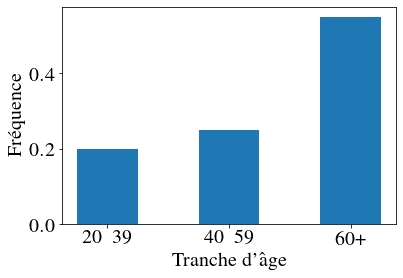
\includegraphics[width=.5\textwidth]{figures/stats/remboursement_age_bars}
%   \caption{Diagramme en bâtons de la fréquence des tranches d'âges dans les
%     données du tableau~\ref{tab:remboursement_data}.}
%   \label{fig:remboursement_age_bars}
% \end{figure}
\begin{figure}[h]
  \centering
    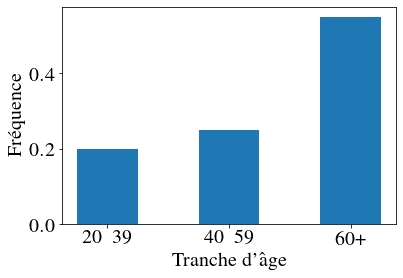
\includegraphics[width=.5\textwidth]{figures/stats/remboursement_age_bars}
  \caption{Diagramme en bâtons de la fréquence des tranches d'âges dans les
    données de remboursement.}
  \label{fig:remboursement_age_bars}
\end{figure}

Dans le cas d'une variable continue, la constitution des classes de valeurs
d'une série statistique est une étape importante. La \textbf{règle de Sturges}
propose de découper les valeurs observées en $k = \lfloor 1 + \log_2(n)\rfloor$
intervalles de même taille $\frac{\max(x_i) - \min(x_i)}{k}$. Cependant, cette
règle suppose que la variable analysée suive une distribution gaussienne ; elle
n'est pas appropriée, par exemple, si les valeurs s'étalent sur plusieurs
échelles de grandeur, auquel cas une transformation logarithmique s'imposera.

% Cela nous permet ensuite de construire une \textbf{table des fréquences} qui
% associe à chaque classe de valeurs la fréquence de cette valeur dans la
% population observée.

\begin{exemple}
  Prenons par exemple, 31 observations de la température minimale (en
  \si{\celsius}) pour la station météo de Paris-Montsouris, telles que relevées
  dans la première colonne de la table~\ref{tab:meteo_data}.

  Nous disposons de $n=31$ observations, qu'il s'agit, en appliquant la règle de
  Sturges, de grouper en 5 intervalles d'amplitude 2,24\si{\celsius}. La table
  des fréquences des températures minimales est donnée dans le
  tableau ci-dessous : \par % ~\ref{tab:meteo_tmin_freq}.
  % \begin{table}[h]

    \centering
    \begin{tabular}[h]{|l|c|c|c|c|c|} \hline 
      T min (\si{\celsius}) & < -0,16 & -0,16 -- 2,08 & 2,08 -- 4,32 & 4,32 -- 6,56 & > 6,56 \\ \hline 
      Fréquence & 0,19 & 0,19 & 0,29 & 0,10 & 0,23 \\ \hline
    \end{tabular}

  %   \caption{Table des fréquences des températures minimales du tableau~\ref{tab:meteo_data}.}
  %   \label{tab:meteo_tmin_freq}
  % \end{table}
\end{exemple}

Pour une variable continue, la table des fréquences peut être traduite en
\textbf{histogramme,} comme illustré sur la figure~\ref{fig:meteo_tmin_hist}.

Utiliser des fréquences plutôt que des comptes permet de comparer des
populations de taille différente. De plus, la distribution des fréquences
d'une série statistique de la variable $x$, représentée visuellement par un
histogramme, peut être considérée comme une approximation de la distribution de
la probabilité de cette variable dans la population.

\begin{figure}[h]
  \centering
  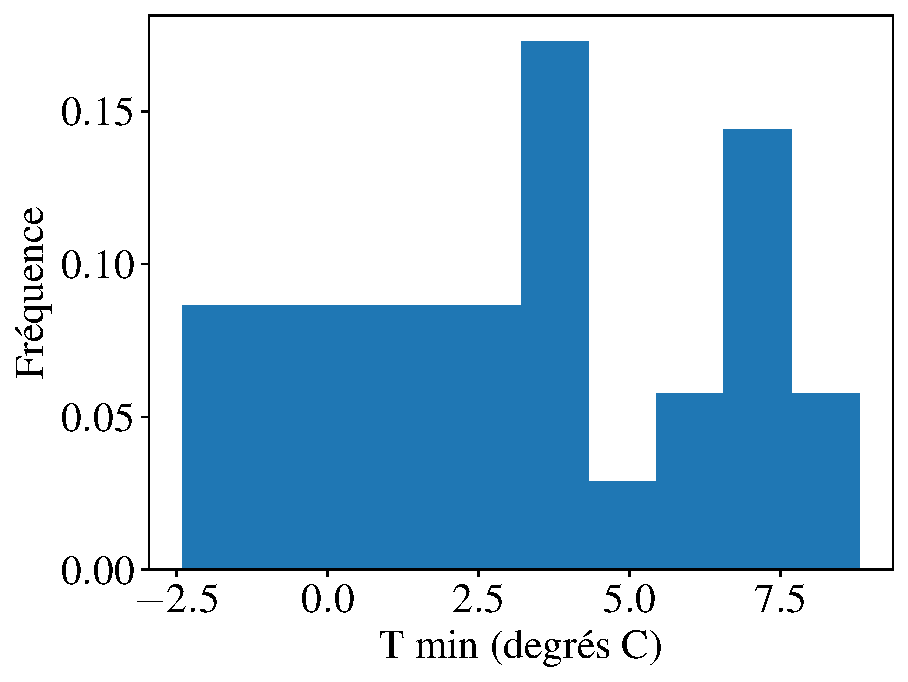
\includegraphics[width=.5\textwidth]{figures/stats/meteo_tmin_hist}
  \caption{Histogramme des températures minimales dans le
    tableau~\ref{tab:meteo_data}.}
  \label{fig:meteo_tmin_hist}
\end{figure}


\paragraph{Fréquences cumulées} 
On peut aussi choisir de représenter plutôt les \textbf{fréquences cumulées.} 

\begin{exemple}
  Pour notre série de températures minimales, la table des fréquences cumulées
  est donnée dans le tableau ci-dessous : \par % ~\ref{tab:meteo_tmin_cumul_freq}.
  % \begin{table}[h]

    \centering
    \begin{tabular}[h]{|l|c|c|c|c|c|} \hline 
      T min (\si{\celsius}) & < -0,16 & < 2,08 & < 4,32 & < 6,56 & < 8,80 \\ \hline 
      Fréquence & 0,19 & 0,38 & 0,67 & 0,77 & 1,0 \\ \hline
      T min (\si{\celsius}) & > -2,40 & > -0,16 & > 2,08 & > 4,32 & > 6,56 \\ \hline 
      Fréquence & 1,0 & 0,81 & 0,62 & 0,33 & 0,23 \\ \hline
    \end{tabular}

  %   \caption{Table des fréquences cumulées pour les températures minimales 
  %     du tableau~\ref{tab:meteo_data}.}
  %   \label{tab:meteo_tmin_cumul_freq}
  % \end{table}
\end{exemple}

Une table des fréquences cumulées croissantes et décroissantes peut
directement être traduite en \textbf{courbes des fréquences cumulées,} comme
illustré sur la figure~\ref{fig:meteo_tmin_cumul_freq}.
\begin{figure}[h]
  \centering
  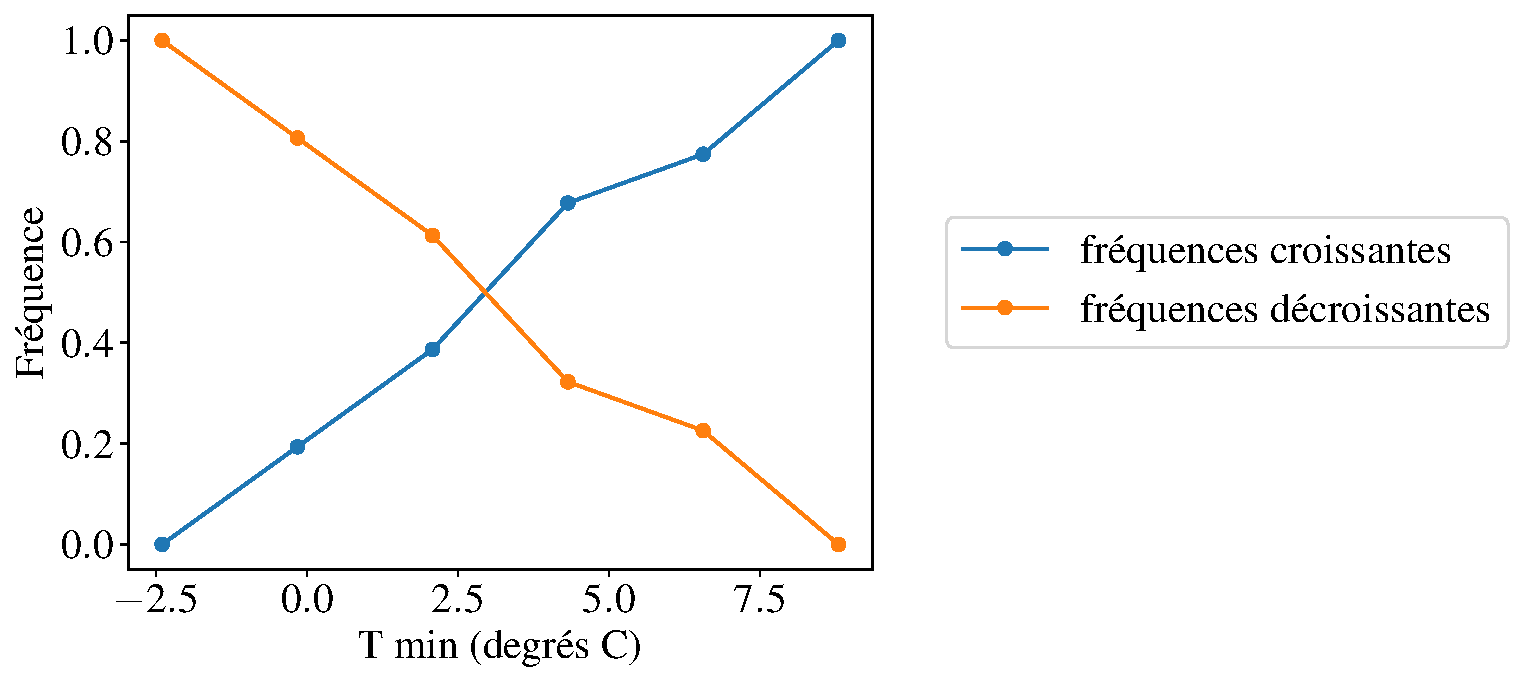
\includegraphics[width=.8\textwidth]{figures/stats/meteo_tmin_cumul_freq}
  \caption{Courbes des fréquences cumulées pour les températures minimales du
    tableau~\ref{tab:meteo_data}.}
  \label{fig:meteo_tmin_cumul_freq}
\end{figure}

\subsection{Indicateurs numériques}
Enfin, des \textbf{indicateurs numériques} permettent de compléter cette
description. On distinguera les \textbf{indicateurs de tendance centrale} qui
indiquent l'ordre de grandeur des valeurs de la série statistique et où ces
valeurs se rassemblent, des \textbf{indicateurs de dispersion} qui indiquent
l'étalement de ces valeurs.

\paragraph{Indicateurs de tendance centrale} Les indicateurs de tendance centrale comportent :
\begin{itemize}
\item la \textbf{moyenne arithmétique} 
\[\bar x = \frac1n \sum_{i=1}^n x_i,\]
La  moyenne arithmétique peut être très sensible à la présence de valeurs aberrantes.
\item la \textbf{médiane,} qui correspond à une fréquence cumulée de 50\%, 
\item le \textbf{mode,} qui est la valeur la plus fréquente dans la série
  statistique. Le mode n'a réellement de sens que pour une variable discrète ;
  dans le cas d'une variable continue, on parlera plutôt, lorsque la série est
  classée, de \textbf{classe modale} qui est la classe la plus fréquente.
\end{itemize}

\begin{exemple}
  Pour notre série de températures minimales,
  \begin{itemize}
  \item la moyenne arithmétique vaut $3,2 \si{\celsius}$ ;
  \item la médiane vaut $4 \si{\celsius}$ ;
  \item la classe modale est $2,1$ -- $4,4 \si{\celsius}$.
  \end{itemize}
\end{exemple}

\paragraph{Indicateurs de dispersion} Les indicateurs de dispersion comportent : 
\begin{itemize}
\item la \textbf{variance de la série statistique} 
\[ \text{var}(x_1, x_2, \dots, x_n) = \frac1n \sum_{i=1}^n (x_i - \bar x)^2,\]
\item la \textbf{variance d'échantillonnage} 
  \[ \text{var}^*(x_1, x_2, \dots, x_n) = \frac1{n-1} \sum_{i=1}^n (x_i - \bar
    x)^2,\]
  La variance d'échantillonnage est d'autant plus proche de la variance que le
  nombre d'observations est grand. Nous verrons dans la
  section~\ref{sec:unbiased_variance_estimation} qu'il s'agit d'une estimation
  \textbf{non-biaisée} de la variance de la population.
\item l'\textbf{écart-type} qui est la racine carrée de la variance, 
\item le \textbf{coefficient de variation} 
  \[ \text{CV}(x_1, x_2, \dots, x_n) = \frac{\text{var}(x_1, x_2, \dots, x_n)}{\bar
      x}\]
  Le coefficient de variation permet d'apprécier la variabilité d'une variable
  en fonction de sa valeur moyenne, et n'a de sens que pour une variable donnée
  sur une échelle dotée d'un zéro absolu, c'est-à-dire dans laquelle une valeur
  de $2z$ peut effectivement être considérée comme deux fois plus qu'une valeur
  de $z$ (ce n'est pas le cas pour une température en degrés Celsius :
  10\si{\celsius} n'est pas « deux fois plus chaud » que 5 \si{\celsius}). De
  plus, il est numériquement instable quand $\bar x$ est proche de 0.
\end{itemize}
\pagebreak
\begin{exemple}
  La variance de notre série de températures minimales vaut $10,02 \si{\celsius^2}$,
  tandis que la variance d'échantillonage vaut $10,36 \si{\celsius^2}$. Les
  écarts-types correspondants valent tous les deux $3,2 \si{\celsius}$.  Le
  coefficient de variation n'a pas de sens en degrés Celsius.
\end{exemple}
\paragraph{Remarques}
\begin{itemize}
\item L'écart-type d'une variable, qui s'exprime dans la même unité que la
  variable, est beaucoup plus facile à interpréter que la variance. On donne
  plus facilement un sens à $3,2 \si{\celsius}$ qu'à $10,02 \si{\celsius^2}$.
\item L'écart-type est utilisé pour définir une erreur de mesure. Imaginons que
  l'on prenne 10 fois la même mesure, obtenant ainsi une population de 10
  mesures, de moyenne arithmétique $m$ et d'écart-type $\sigma$ ; on rapporte
  alors une valeur de $m \pm \sigma$. Cette remarque est une brève incursion
  dans le domaine de la \textit{métrologie}.
\end{itemize}

Enfin, les \textbf{quantiles} permettent aussi de déterminer la dispersion
d'une variable. Les $q$-quantiles divisent les valeurs prises par la variable
en $q$ intervalles de mêmes fréquences. Le $p$-ème $q$-quantile de
$(x_1, x_2, \dots, x_n)$ est défini comme la valeur $Q_p^q$ telle que 
\[\text{Freq}(x \leq Q_p) = \frac{p}{q}.\]

Lorsque $q=4,$ on parle de \textbf{quartiles.} Lorsque $q=10,$ on parle de
\textbf{déciles.}

\begin{exemple}
  Les trois quartiles de notre série de températures minimales sont
  $0,8 \si{\celsius}$, $4,0 \si{\celsius}$ et $5,6 \si{\celsius}$ : 25\% des
  valeurs observées sont inférieures à $0,8 \si{\celsius}$, 50\% sont inférieures
  à 4,0 \si{\celsius} et 75\% sont inférieures à $5,6 \si{\celsius}$. Le deuxième
  quartile correspond bien à la médiane.
\end{exemple}

Une \textbf{boîte à moustaches} (ou \textit{boxplot}) permet de résumer
visuellement ces indicateurs, comme illustré sur la
figure~\ref{fig:meteo_tmin_boxplot}. La boîte à moustaches est composée d'un
rectangle, d'une largeur arbitraire et délimité en bas par la valeur du premier
quartile et en haut par la valeur du troisième quartile ; d'une barre
horizontale au niveau de la médiane ; et de deux segments joignant chacun les
extrémités du rectangle aux valeurs les plus extrêmes. Représenter les valeurs
prises par la variable par un nuage de points superposé à ce rectangle permet
d'en faciliter l'interprétation.

\begin{figure}[h]
  \centering
  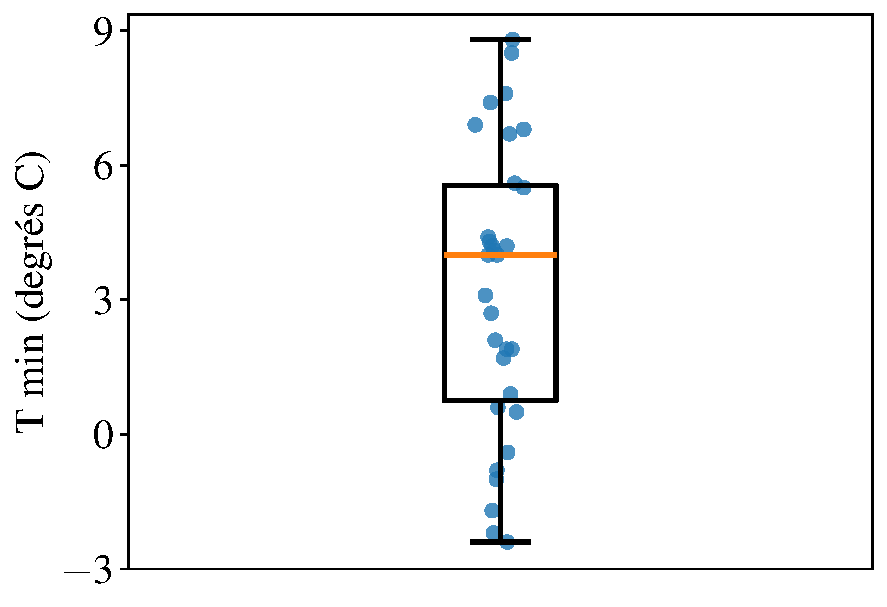
\includegraphics[width=.5\textwidth]{figures/stats/meteo_tmin_boxplot}
  \caption{Boîte à moustaches des températures minimales du
    tableau~\ref{tab:meteo_data}.}
  \label{fig:meteo_tmin_boxplot}
\end{figure}

\section{Statistique descriptive bidimensionelle}
Il s'agit ici de mettre en évidence une éventuelle \textbf{liaison,}
c'est-à-dire une variabilité simultanée, entre deux variables statistiques $x$
et $y$, observées sur $n$ individus, à travers les séries statistiques
$(x_1, x_2, \dots, x_n)$ et $(y_1, y_2, \dots, y_n).$

Cette liaison peut être causale ou non. Mettre en évidence une causalité est
délicat, et dépasse le cadre de ce cours.

Comprendre la liaison entre deux variables nous permet de comprendre 
\begin{itemize}
\item Si une variable peut dépendre d'une autre : la température minimale
  dépend-elle de l'ensoleillement ?
\item Si une variable peut permettre de prédire une autre : la température
  minimale permet-elle de prédire la température maximale ?
\item Si une variable peut être remplacée par une autre : ai-je besoin de
  prendre en compte et la température minimale et la température maximale, ou
  la température moyenne suffit-elle ?
\end{itemize}

\subsection{Liaison entre deux variables quantitatives}

\paragraph{Nuage de points}
Pour visualiser la liaison entre deux variables quantitatives, on utilise
généralement un \textbf{nuage de points}. Si $x$ et $y$ sont homogènes,
c'est-à-dire exprimées dans la même unité, on utilisera la même échelle sur les
deux axes, comme sur la figure~\ref{fig:meteo_tmin_tmax}. Sinon, on préfèrera
généralement centrer et réduire les variables au préalable, comme sur la
figure~\ref{fig:meteo_tmin_vent} : 
\[
  x_i \leftarrow \frac{x_i - \bar x}{\sigma_x} \qquad \text{avec } \bar x = \frac{1}{n} \sum_{i=1}^n x_i 
  \text{ et } \sigma_x = \sqrt{\frac{1}{n} \sum_{i=1}^n(x_i - \bar x)^2}.
\]

\begin{figure}[h]
  \centering
  \begin{subfigure}[t]{0.49\textwidth}
    \centering
    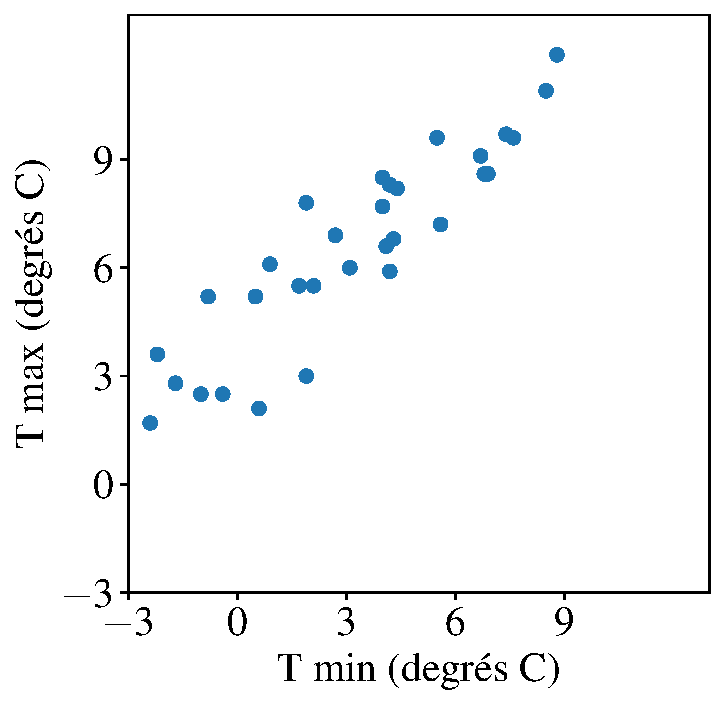
\includegraphics[width=.7\textwidth]{figures/stats/meteo_tmin_tmax}
    \caption{Températures maximales vs minimales.}
    \label{fig:meteo_tmin_tmax}
  \end{subfigure} \hfill
  \begin{subfigure}[t]{0.49\textwidth}
    \centering
    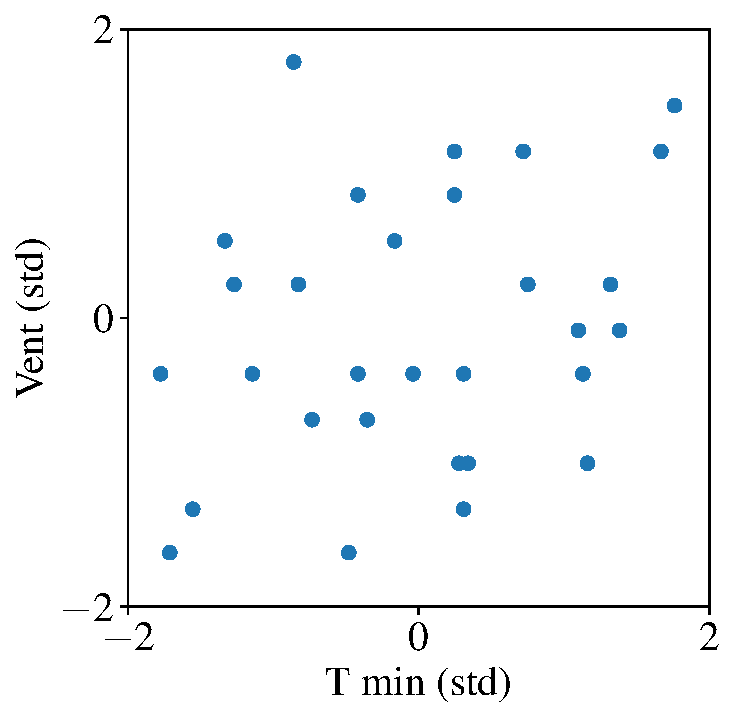
\includegraphics[width=.7\textwidth]{figures/stats/meteo_tmin_vent}
    \caption{Vent vs températures minimales.}
    \label{fig:meteo_tmin_vent}
  \end{subfigure}
  \caption{Nuages de points pour des paires de variables du
    tableau~\ref{tab:meteo_data}.}
\end{figure}


\paragraph{Indicateurs de liaison entre deux variables quantitatives}
Pour quantifier la liaison entre deux variables quantitatives, on utilise
principalement
\begin{itemize}
\item \textbf{la covariance}
\[\text{cov}(x, y) = \frac1n \sum_{i=1}^n (x_i - \bar x) (y_i - \bar y).\]
\item \textbf{le coefficient de corrélation de Pearson,} qui est égal à la
  covariance entre les variables centrées réduites, et compris entre $-1$ et $1$ :
\[r(x, y) = \frac1n \frac{\sum_{i=1}^n (x_i - \bar x) (y_i - \bar y)}{\sigma_x \sigma_y}.\]
\end{itemize}

À noter que la covariance et le coefficient de corrélation de Pearson mesurent
des liaisons \textit{linéaires} entre deux variables. Une corrélation de
Pearson proche de 1 ou de -1 indique une relation linéaire ; une corrélation de
Pearson proche de 0 indique une absence de corrélation. D'autres mesures, comme
l'information mutuelle (hors cadre de ce cours), permettent de mesurer des
liaisons \textit{non-linéaires}. 

\begin{exemple}
  Pour les données du tableau~\ref{tab:meteo_data}, la covariance entre la
  température minimale et la température maximale vaut $7,69 \si{\celsius^2}$ ;
  leur corrélation de Pearson vaut 0,91. La corrélation de Pearson entre vent
  et température minimale vaut 0,28. La figure~\ref{fig:pearson} illustre le
  rapport entre corrélation de Pearson et nuage de points.
\end{exemple}
\begin{figure}[h]
  \centering
    \begin{subfigure}[t]{0.24\textwidth}
      \centering
      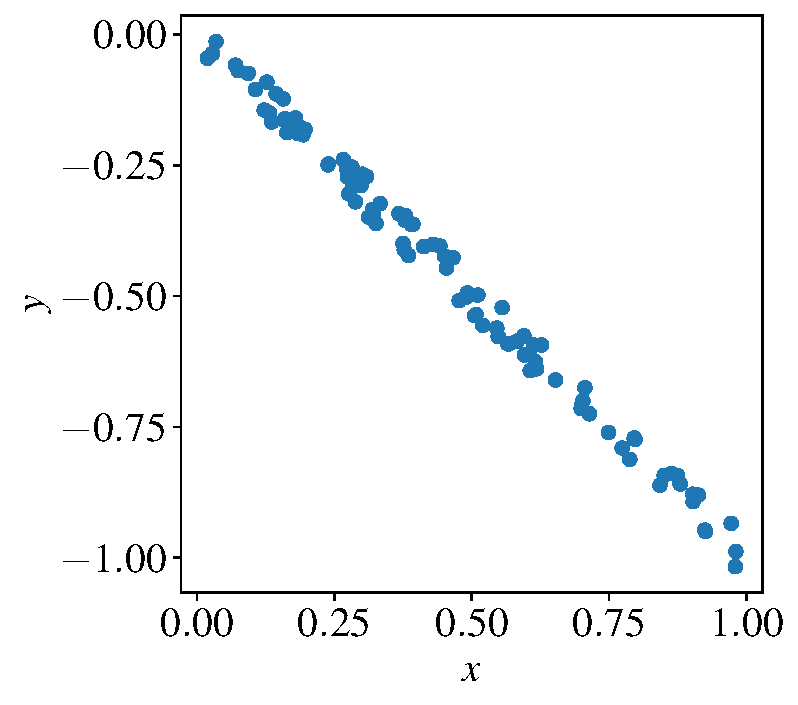
\includegraphics[width=\textwidth]{figures/stats/pearson_3}
      \caption{r(x, y) = -1,00.}
    \end{subfigure} \hfill
    \begin{subfigure}[t]{0.24\textwidth}
      \centering
      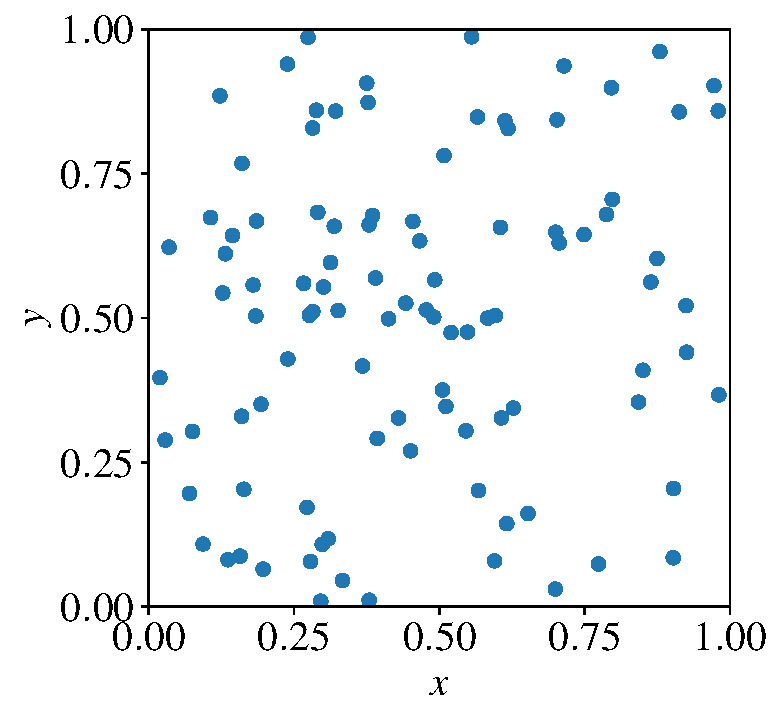
\includegraphics[width=\textwidth]{figures/stats/pearson_0}
      \caption{r(x, y) = 0,03.}
    \end{subfigure} \hfill
    \begin{subfigure}[t]{0.24\textwidth}
      \centering
      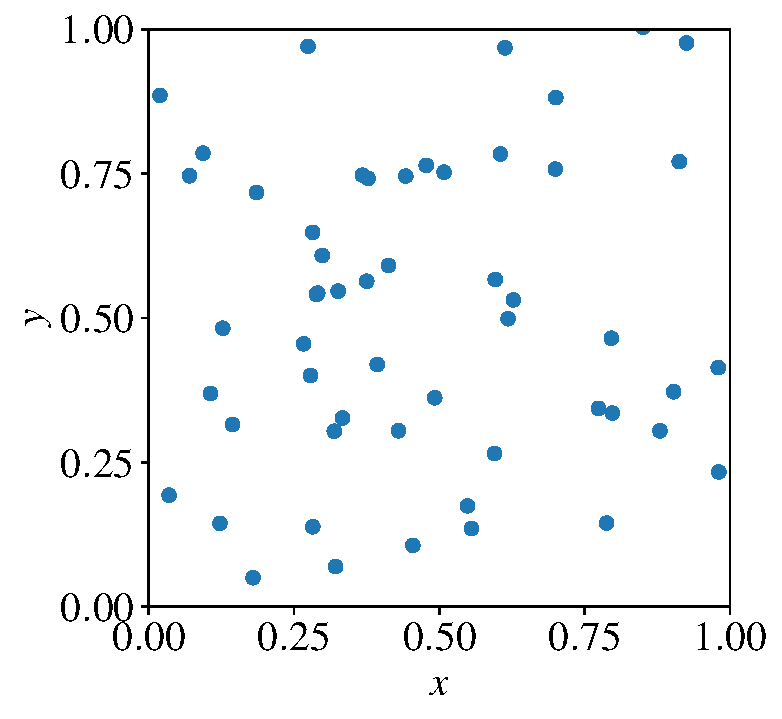
\includegraphics[width=\textwidth]{figures/stats/pearson_2}
      \caption{r(x, y) = 0,53.}
    \end{subfigure} \hfill
    \begin{subfigure}[t]{0.24\textwidth}
      \centering
      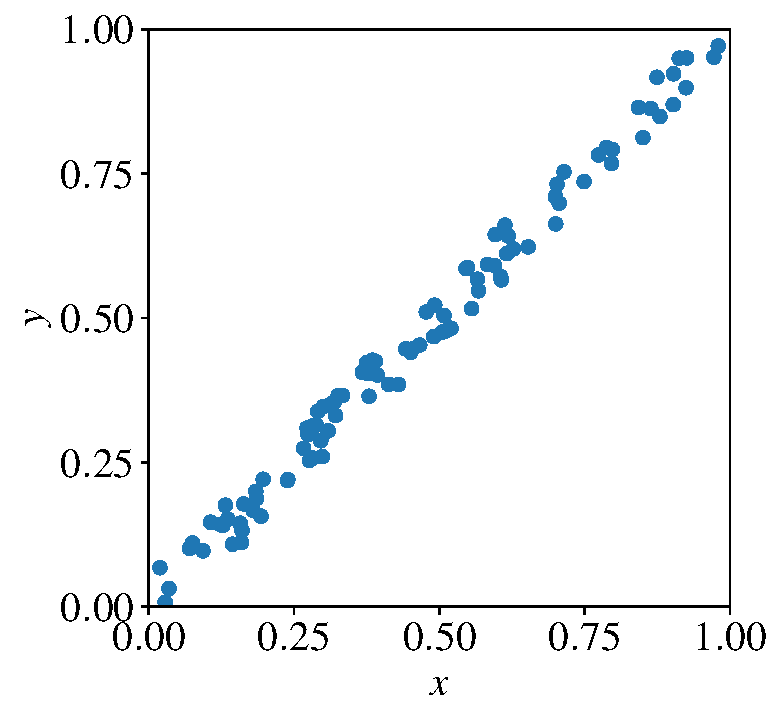
\includegraphics[width=\textwidth]{figures/stats/pearson_1}
      \caption{r(x, y) = 1,00.}
    \end{subfigure} \hfill
  \caption{Nuages de points entre deux variables simulées et leur corrélation de Pearson.}
  \label{fig:pearson}
\end{figure}

\paragraph{Indicateurs de liaison entre une variable qualitative et une variable quantitative}
Pour étudier la liaison entre une variable qualitative $x$, ayant $K$ modes (ou
valeurs différentes) dans la série statistique $(x_1, x_2, \dots, x_n),$ et une
variable quantitative $y,$ on considère que la variable $x$ permet de définir
$p$ sous-populations. Il s'agit alors d'évaluer s'il existe des différences,
pour la variable $y$, entre ces sous-populations.

Visuellement, on utilisera une série de boîtes à moustaches, comme illustré sur
la figure~\ref{fig:remboursement_rembourses_age}.

% \begin{figure}[h]
%   \centering
%   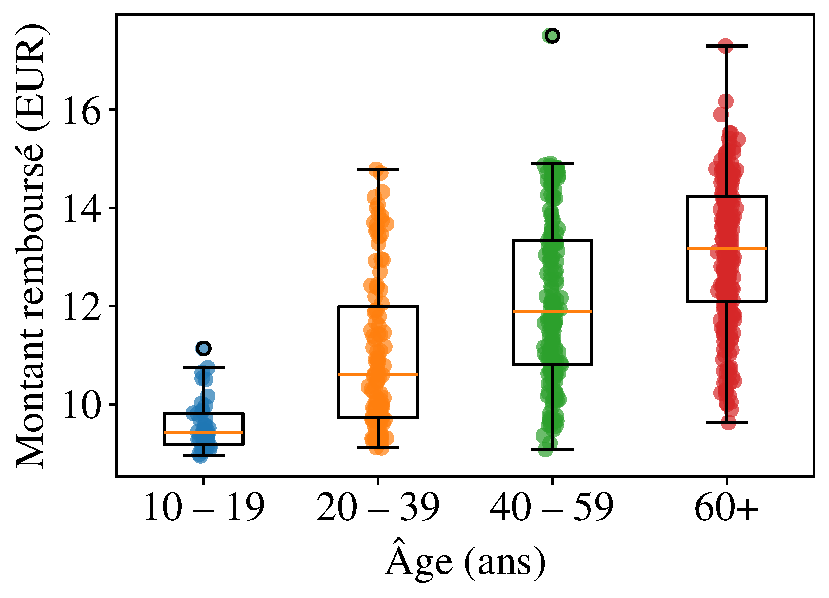
\includegraphics[width=.5\textwidth]{figures/stats/remboursement_rembourses_age}
%   \caption{Montants remboursés par acte, par tranche d'âge, pour les données du
%     tableau~\ref{tab:remboursement_data}.}
%   \label{fig:remboursement_rembourses_age}
% \end{figure}
\begin{figure}[h]
  \centering
  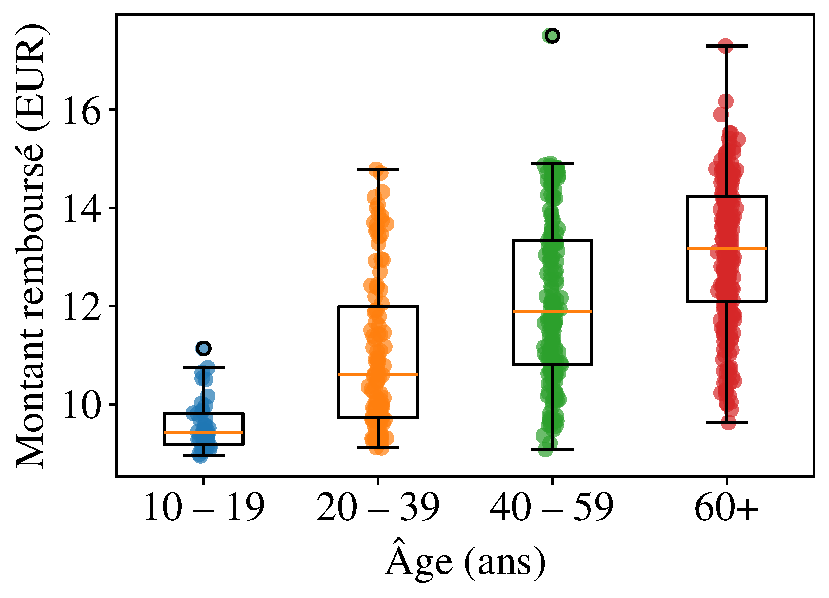
\includegraphics[width=.5\textwidth]{figures/stats/remboursement_rembourses_age}
  \caption{Montants remboursés par acte, par tranche d'âge, pour les données de
    remboursement.}
  \label{fig:remboursement_rembourses_age}
\end{figure}

La \textbf{variance expliquée} par $x$ de $y$ est la moyenne des carrés des écarts
entre la moyenne de $y$ dans chaque sous-population et la moyenne de $y$ dans
toute la population, pondérée par la taille des sous-populations :
\[
  \sigma_E^2 = \frac1n \sum_{k=1}^K n_k (\bar{y}_k - \bar{y})^2,
\]
où $\bar{y}_k$ est la moyenne de $y$ dans la sous-population $k$ et $\bar{y}$
la moyenne de $y$ dans la population totale.

La \textbf{variance résiduelle} est la moyenne des variances des
sous-populations, pondérées par leur taille :
\[
  \sigma_R^2 = \frac1n \sum_{k=1}^K n_k \sigma_k^2, 
\]
où $n_k$ est le nombre d'individus dans la sous-population $k$ et $\sigma_k^2$
est la variance de $y$ dans cette sous-population.


On peut montrer que $\sigma_y^2 = \sigma_R^2 + \sigma_E^2.$

Le \textbf{rapport de corrélation} est la part de variation de $y$ expliquée
par $x$. Compris entre 0 et 1, il est d'autant plus élevé que la liaison entre
les deux variables est forte :
\[
e^2  = \frac{\sigma_E^2}{\sigma_y^2}.
\]
\begin{exemple}
% Pour les montants remboursés par acte du tableau~\ref{tab:remboursement_data},
% la variance de ces montants est de 3,65, tandis que la variance expliquée par
% l'âge est de 1,37 (en euros au carré), ce qui donne un rapport de corrélation
% de 0,38.
  Pour les montants remboursés par acte de nos données de remboursement, la
  variance de ces montants est de $3,30$\texteuro$^2$, tandis que la variance
  expliquée par l'âge est de $1,09$\texteuro$^2$, ce qui donne un rapport de
  corrélation de $0,33.$ 
\end{exemple}

\paragraph{Indicateurs de liaison entre deux variables qualitatives}
Pour étudier la liaison entre une variable qualitative $x$, ayant $K$ modes (ou
valeurs différentes) dans la série statistique $(x_1, x_2, \dots, x_n),$ et une
variable qualitative $y$, ayant $L$ modes dans la série statistique
$(y_1, y_2, \dots, y_n),$ on utilise généralement une \textbf{table de
  contingence} $A$ de taille $K \times L.$ Il s'agit de compter, pour chaque
mode de $x$ et chaque mode de $y$, combien d'individus présentent ces deux
modes : $A_{ij}$ est le nombre d'invididus pour lesquels $x = i$ et $y = j$.

Si l'on appelle $N = \sum_{k=1}^K \sum_{l=1}^L A_{kl}$ le nombre total
d'individus, $N_{i.} = \sum_{l=1}^L A_{il}$ le nombre d'individus dans la ligne
$i$ et $N_{.j} = \sum_{k=1}^K A_{kj}$ le nombre d'individus dans la colonne $j$,
alors l'absence de liaison entre $x$ et $y$ se traduit par 
\[
  \frac{N_{ij}}{N} = \frac{N_{i.}}{N}
  \frac{N_{.j}}{N} \text{ pour tout } 
  1 \leq i \leq K, 1 \leq j \leq L.
\]
L'écart entre les valeurs prises de part et d'autre de cette égalité se mesure
grâce à la \textbf{distance du chi2}, définie par 
\[
d_{\chi^2} = \sum_{i=1}^K \sum_{j=1}^L  \frac{\left( A_{ij} - 
    \frac{N_{i.}N_{.j}}{N} \right)^2}{\frac{N_{i.}N_{.j}}{N}}
\]

\begin{exemple}
  La table de contingence pour les variables « âge » et « région » des données
  de remboursement est donnée dans le
  tableau~\ref{tab:remboursement_age_region}. La distance du chi2 pour cette
  table de contingence est de 11,21, ce qui suggère une dépendance entre les
  variables « âge » et « région » dans les données.
\end{exemple}


  \begin{table}[h]
    \centering
    \begin{tabular}[h]{|c|c|c|c|c|c|c|c|c|c|c|c|c|c|}
      \hline
      & \multicolumn{13}{|c|}{Région} \\ \hline
      {Âge} & 5 & 11 & 24 & 27 & 28 & 32 & 44 & 52 & 53 & 75 & 76 & 84 & 93 \\ \hline
      0--19 & 3 & 5 & 3 & 3 & 3 & 3 & 4 & 3 & 2 & 3 & 3 & 4 & 4 \\ \hline
      20--39 & 8 & 18 & 4 & 7 & 4 & 9 & 11 & 6 & 4 & 7 & 8 & 10 & 11 \\ \hline
      40--59 & 11 & 26 & 11 & 13 & 13 & 16 & 15 & 10 & 8 & 12 & 17 & 15 & 19 \\ \hline
      $>$ 60 & 15 & 31 & 18 & 16 & 21 & 21 & 22 & 12 & 12 & 19 & 24 & 23 & 26 \\ \hline
    \end{tabular}
    \caption{Table de contingence pour l'âge et la région des données 
      de remboursement.}
    \label{tab:remboursement_age_region}
  \end{table}

% Nous verrons dans la PC1 comment transformer cette distance en
% un test statistique de dépendance.

% \begin{table}[h]
%   \centering
%   \begin{tabular}[h]{|c|c|c|c|c|c|c|c|c|c|c|}
%     \hline
%     & \multicolumn{10}{|c|}{Région} \\ \hline
%     {Âge} & 5 & 11 & 24 & 27 & 32 & 44 & 75 & 76 & 84 & 93 \\ \hline
%     20--39 & 1 & 1 & 0 & 0 & 2 & 0 & 0 & 0 & 0 & 0 \\ \hline
%     40--59 & 0 & 1 & 0 & 0 & 1 & 1 & 0 & 1 & 1 & 0 \\ \hline
%     $>$ 60 & 1 & 1 & 1 & 1 & 2 & 1 & 1 & 2 & 0 & 1 \\ \hline
%   \end{tabular}
%   \caption{Table de contingence pour l'âge et la région des données 
%     du tableau~\ref{tab:remboursement_data}.}
%   \label{tab:remboursement_age_region}
% \end{table}

La table de contingence peut être visualisée grâce à deux \textbf{diagrammes en
  barres empilées} : on peut choisir de visualiser, pour chaque mode de $x$, la
proportion relative des modes de $y$, ou inversement, pour chaque mode de $y$,
la proportion relative des modes de $x$. Ces deux choix sont illustrés sur les
figures~\ref{fig:remboursement_age_region_lines}
et~\ref{fig:remboursement_age_region_cols} respectivement.

\begin{figure}[h]
  \centering
  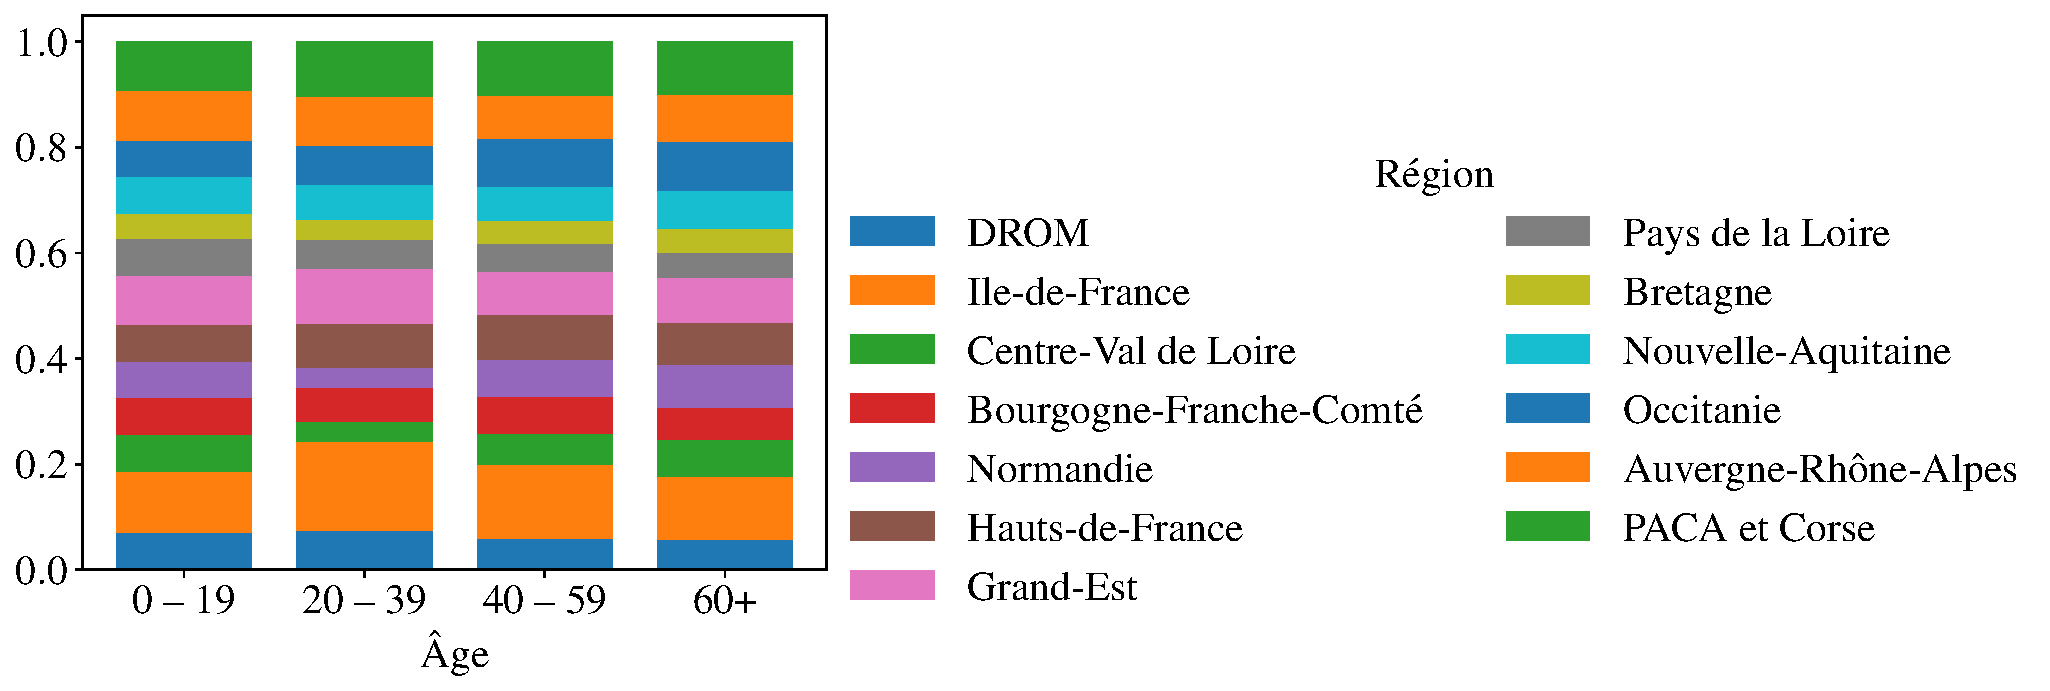
\includegraphics[width=\textwidth]{figures/stats/remboursement_age_region_lines}
  \caption{Diagramme en barres représentant, pour chaque tranche d'âges, la
    proportion relative d'individus de chaque région dans la table de
    contingence du tableau~\ref{tab:remboursement_age_region}.}
  \label{fig:remboursement_age_region_lines}
\end{figure}

\begin{figure}[h]
  \centering
  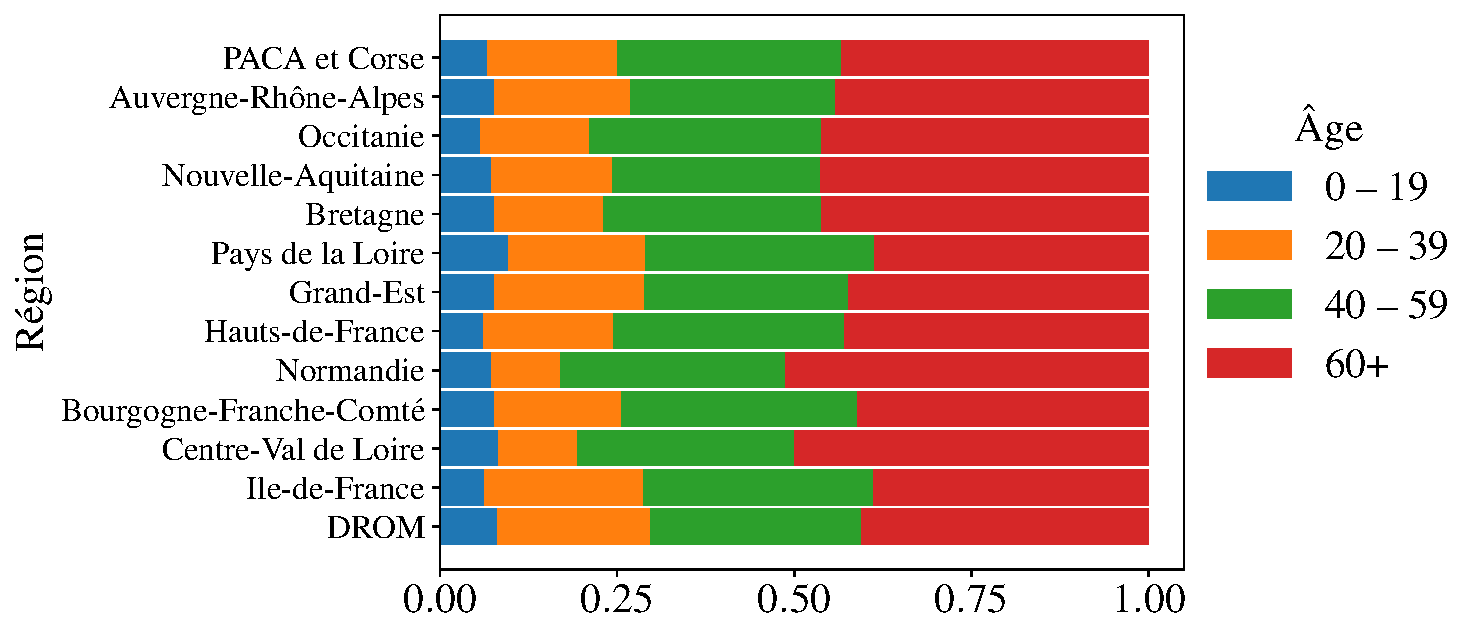
\includegraphics[width=\textwidth]{figures/stats/remboursement_age_region_cols}
  \caption{Diagramme en barres représentant, pour chaque région, la proportion
    relative d'individus de chaque tranche d'âge dans la table de contingence du
    tableau~\ref{tab:remboursement_age_region}.}
  \label{fig:remboursement_age_region_cols}
\end{figure}

\clearpage
%-*- coding: utf-8 -*-
\section{QCM}
\paragraph{Question 1.} On s'intéresse aux hospitalisations pour une certaine
maladie. Comment visualiser la liaison entre la durée du séjour à l'hôpital et
l'âge des patients, la première étant donnée en nombre de jours et le second
par tranches ?
\begin{itemize}
	\item[$\square$] Par un nuage de points 
	\item[$\square$] Par un diagramme en barres
	\item[$\square$] Par une série de boîtes à moustaches
\end{itemize}

\paragraph{Question 2.} L'image ci-dessous représente un nuage de points entre
le diamètre de fleurs et la hauteur de leur tige. Leur coefficient de
corrélation de Pearson est plutôt proche de...
\begin{itemize}
	\item[$\square$] $- 0,35$
	\item[$\square$] $+ 0,35$
	\item[$\square$] $- 0,85$
	\item[$\square$] $+ 0,85$
	\item[$\square$] $- 0,95$
	\item[$\square$] $+ 0,95$
	\item[$\square$] $- 0,50$
	\item[$\square$] $+ 0,50$
\end{itemize}

\vspace{-13em}
\begin{center}
	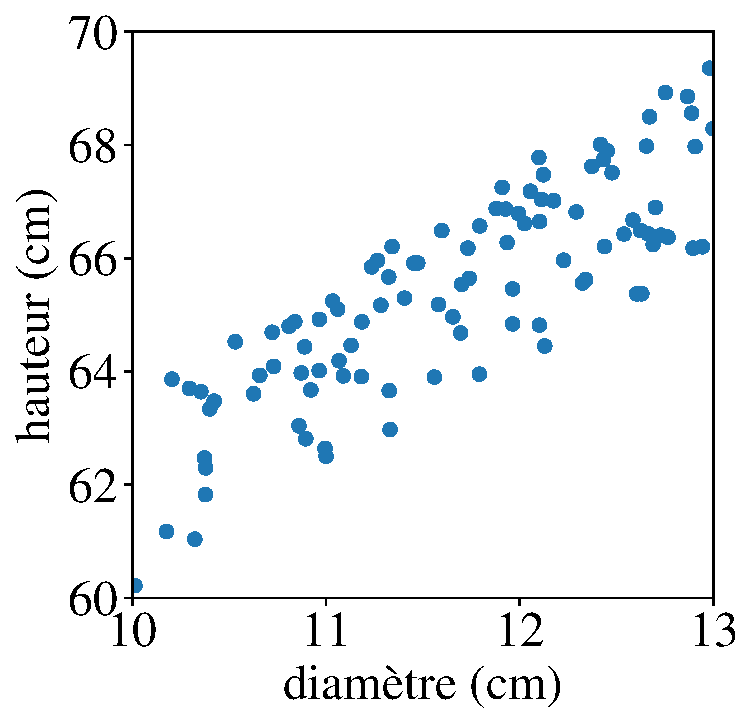
\includegraphics[width=0.35\textwidth]{figures/pearson_example}
\end{center}



\section*{Solution}
{%
	\noindent
	\rotatebox[origin=c]{180}{%
		\noindent
		\begin{minipage}[t]{\linewidth}
			\paragraph{Question 1.} Une série de boîtes à moustaches est plus appropriée
			pour visualiser la relation entre une variable quantitative (durée du séjour)
			et une variable qualitative (âge par
			tranches). Cf. figure~\ref{fig:remboursement_rembourses_age}.\newline
			
			\paragraph{Question 2.} $r \approx 0,85.$ On peut voir à la « pente » que la
			corrélation est positive. La situation est intermédiaire entre celle des
			figures 2.6(\textsc{C}) $(r=0,50)$ et 2.6(\textsc{D}) $(r=1,00)$. Une
			corrélation de $0,95$ serait plus proche de la figure~\ref{fig:pearson}(\textsc{D}) que de
			celle donnée ci-dessus. Remarquez ici que les données ne sont pas homogènes, au
			sens où elles ont des échelles de valeurs différentes, contrairement à ce qui
			est représenté sur la figure~\ref{fig:pearson} ; cela ne change pas l'interprétation de la
			corrélation.
		\end{minipage}%
	}%
	
	
	%%% Local Variables:
	%%% mode: latex
	%%% TeX-master: "../../sdd_2025_poly"
	%%% End:



%%% Local Variables:
%%% mode: latex
%%% TeX-master: "../sdd_2025_poly"
%%% End:
\clearpage 

\chapter{Estimation}
%-*- coding: utf-8 -*-
\label{chap:estimation}

\paragraph{Notions :} échantillon aléatoire, estimateur, estimation, biais d'un
estimateur, convergence d'un estimateur, estimation par maximisation de la
vraisemblance, estimation de Bayes.
\paragraph{Objectifs pédagogiques :}
\begin{itemize}
\setlength{\itemsep}{3pt}
\item Choisir un estimateur, en particulier en déterminant des propriétés
  telles que son biais ou sa précision.
\item Proposer un estimateur, en particulier par maximisation de la
  vraisemblance.
\end{itemize}


\section{Inférence statistique}
Alors que la statistique descriptive se contente de \textit{décrire} une
population ou un échantillon de celle-ci, l'inférence statistique cherche à
tirer des conclusions sur une population à partir de l'étude d'un échantillon
de celle-ci, tout en évaluant le niveau de confiance qui peut leur être accordé.

\subsection{Échantillonnage en population finie}
\label{ref:echantilonnage}

Lorsque la population à étudier possède un nombre fini $N$ d'individus trop élevé pour qu'il soit possible
de tous les observer, on en étudie alors un sous-ensemble de taille $n < N$, appelé \textbf{échantillon}. On parle alors de
\textbf{sondage}, par opposition à un \textbf{recensement}, qui consiste à
étudier tous les individus d'une population.

\paragraph{Échantillonnage aléatoire}
Notons $U$ la population d'intérêt et $\mathcal{P}(U)$ l'ensemble de ses parties. Afin d'induire les caractéristiques de $U$ à partir d'un unique échantillon $s \subset U$ tout en étant capable de contrôler le niveau de précision des résultats fournis (qui serait parfait en cas de recensement), la théorie des sondages s'appuie sur la sélection aléatoire de ce sous-ensemble d'individus. Pour cela, une loi de probabilité discrète $\PP_S$ est choisie sur l'ensemble $\mathcal{P}(U)$ de tous les échantillons possibles. On définit ensuite un \textit{échantillon aléatoire} $S \sim \PP_S$, dont est tirée une réalisation $s$, qui forme l'échantillon observé.  

\paragraph{Plans de sondage} La loi de probabilité $\PP_S$ définit un plan de sondage aléatoire sans remise. Il est dit \textbf{simple} lorsque $n$ est fixé à l'avance et que tous les échantillons de taille $n$ ont la même probabilité d'être sélectionnés : $$\forall\,s\subset U\qquad \PP_S(s) = \PP(S=s) = \begin{cases} \binom{N}{n}^{-1} & \text{si } \text{Card}(s) = n,\\ 0 & \text{sinon.} \end{cases}$$ Chaque individu a alors une chance $\frac{n}{N}$ d'être tiré.

D'autres techniques d'échantillonnage sont évidemment possibles. Le plan de sondage \textbf{stratifié}, par exemple, repose sur le partitionnement de la population en strates selon
une caractéristique connue (e.g. par tranche d'âge). L'échantillon est
ensuite obtenu en procédant à un échantillonnage aléatoire simple dans chacune des strates. Les individus n'ont alors pas tous la même probabilité d'être tirés : elle dépend de la taille de la strate à laquelle ils appartiennent.

\paragraph{Inférence en population finie}
Dans ce contexte, la statistique inférentielle a pour but d'identifier un ensemble de caractéristiques observables sur la population. Par exemple, si l'on s'intéresse à une variable $x$ prenant les valeurs $(x_i)_{i\in U}$ dans la population, on peut souhaiter évaluer le total $x^* = \sum_{i\in U} x_i$ alors que l'on ne dispose que de la série statistique $(x_i)_{i\in s}$. Si cette dernière est obtenue via un plan aléatoire simple, on peut par exemple utiliser la somme pondérée $\sum_{i \in s} \frac{N}{n} x_i$. Cette quantité est une \textbf{estimation} du total $x^*$. De manière à déterminer avec quelle précision elle s'approche de $x^*$ quel que soit l'échantillon $s$ dont on dispose, on étudie plutôt les propriétés probabilistes de la somme pondérée aléatoire $\sum_{i \in S} \frac{N}{n} x_i$, dite \textbf{estimateur} du total $x^*$.

\paragraph{Représentativité} Avant de tirer des conclusions d'un échantillon
aléatoire, il est important de comprendre s'il est représentatif de la
population étudiée, et d'adapter en conséquence les outils mathématiques d'évaluation des caractéristiques de la population complète. Par exemple, les premières études cliniques démontrant
l'efficacité de l'aspirine pour réduire le risque d'infarctus du myocarde chez
les patients à risque portaient sur des échantillons composés principalement
d'hommes ; ce n'est que bien plus tard que la communauté médicale a réalisé que
l'efficacité est bien moindre chez les femmes. 
En théorie des sondages, on cherche généralement à éviter la représentativité, pour se concentrer sur la collecte des données qui donneront les évaluations les plus précises possibles des caractéristiques de la population. C'est au moment des calculs que le déséquilibre introduit est pris en compte et compensé, par la pondération des observations.

\subsection{Modèle statistique}

{\'E}tant donné le cadre précédemment posé, comment appréhender une population qui n'est pas réellement fixée, mais en perpétuelle évolution ? Plus encore, comment étudier une collection de mesures théoriquement réalisables une infinité de fois, comme lors d'expériences physiques en laboratoire ? 
La modélisation statistique permet d'apporter une réponse à ces questions. Elle s'intéresse aux expériences dites aléatoires qui, menées de manière répétée dans les mêmes conditions contrôlables, ne donnent pas systématiquement le même résultat.

\paragraph{Échantillon aléatoire et échantillon} Deux séries de résultats d'une telle expérience de même taille $n$ constituent deux échantillons $(x_1, x_2, \dots, x_n)$ et $(x^\prime_1, x^\prime_2, \dots, x^\prime_n)$ différents l'un de l'autre. On modélise cette variabilité en
considérant que les observations $x_i$ et $x^\prime_i$ sont la réalisation
d'une même variable aléatoire $X_i$. Le vecteur aléatoire $(X_1, X_2, \dots, X_n)$ représente alors un échantillon-type de taille $n$. Il est appelé \textbf{échantillon aléatoire}, par contraste avec les échantillons $(x_1, x_2, \dots, x_n)$ et $(x^\prime_1, x^\prime_2, \dots, x^\prime_n)$ qui en sont des \textit{réalisations}.

Un \textbf{indicateur statistique} de l'échantillon est alors la réalisation d'une variable aléatoire fonction de l'échantillon aléatoire.

\begin{exemple} La moyenne d'un échantillon
	$\bar{x} = \frac1n \sum_{i=1}^n x_i$ est une réalisation de la variable
	aléatoire
	\[
	M_n = \frac1n \sum_{i=1}^n X_i,
	\]
	qui est une fonction de l'échantillon aléatoire $(X_1, X_2, \dots, X_n)$.
\end{exemple}


\paragraph{Modèle statistique} Un modèle statistique est défini comme un triplet caractérisant notre croyance sur l'aléa observé :
\begin{itemize}
	\item l'ensemble $\XX$ dans lequel le vecteur aléatoire $(X_1, X_2, \dots, X_n)$ prend ses valeurs,
	\item la tribu associée $\Bcal$,
	\item une famille de lois de probabilités sur $(\XX,\Bcal)$ dans laquelle il est supposé que se trouve celle de $(X_1, X_2, \dots, X_n)$.
\end{itemize}
Lorsque la famille de lois est connue et caractérisée par un petit nombre de paramètres (e.g. loi gaussienne, loi de Poisson, etc.), on parle de \textbf{statistique inférentielle paramétrique}. Lorsqu'elle est totalement
inconnue, on parle de \textbf{statistique inférentielle non-paramétrique}.

\paragraph{$n$-échantillon aléatoire}	Dans toute la suite du chapitre, nous supposerons que $X_1,\dots,X_n$ sont des variables aléatoires indépendantes et identiquement distribuées (iid), de même loi qu'une variable aléatoire générique $X$. Le vecteur $(X_1,\dots,X_n)$ est alors appelé $n$-échantillon aléatoire. 


\paragraph{Objectifs de la statistique inférentielle} Dans ce cadre, la statistique inférentielle a pour but d'\textbf{iden\-tifier les lois de probabilité de ces variables aléatoires.} Cela peut prendre les
formes suivantes :
\begin{itemize}
\item L'\textbf{estimation}, qui permet de déterminer les paramètres des lois (paramètre $p$ d'une loi de Bernoulli, indice et paramètre d'échelle d'une loi Gamma) ou certaines de leurs caractéristiques (espérance, variance, moments d'ordre supérieur, quartiles, etc.). C'est le sujet de ce chapitre.
\item Les \textbf{tests d'hypothèse}, qui permettent d'infirmer ou de confirmer des hypothèses faites sur ces lois, leurs paramètres ou leurs
  caractéristiques. Il s'agit par exemple de décider s'il est plausible que
  l'espérance d'une variable soit supérieure à une certaine valeur ; ou qu'une
  variable suive une loi normale. C'est le sujet du chapitre~\ref{chap:tests}. %Ce sujet dépasse le cadre de ce cours. 
\end{itemize}



\section{Estimation ponctuelle}
Soit $(\Omega, \Acal, \PP)$ un espace probabilisé, $E$ un espace mesurable, et
$X$ une variable aléatoire à valeurs dans $E$. En pratique, dans la suite de ce
chapitre, nous considèrerons des variables aléatoires réelles ($E = \RR$ ou une
partie de $\RR$ telle que $\RR_+$ ou $\NN$), mais les idées qui y sont
présentées peuvent être étendues à $\RR^d$ ou à des espaces plus sophistiqués.

Soit $(X_1, X_2, \dots, X_n)$ un échantillon aléatoire de $X$. Les $X_i$ sont
indépendantes et identiquement distribuées, de même loi $\PP_X$ que $X.$ Soit
$(x_1, x_2, \dots, x_n)$ un échantillon, autrement dit une réalisation de cet
échantillon aléatoire. Soit enfin $\theta \in \RR$ une quantité déterministe
(autrement dit, il ne s'agit pas d'une variable aléatoire), qui dépend
uniquement de $\PP_X.$ Le but de l'estimation ponctuelle est d'approcher au
mieux la valeur de $\theta$.

Par exemple, si l'on fait l'hypothèse que $X$ suit une loi exponentielle (nous
sommes donc dans un contexte de statistique inférentielle paramétrique),
$\theta$ peut être le paramètre de cette loi, mais aussi un de ses moments, un
quantile, etc.


\subsection{Définition d'un estimateur}
On appelle \textbf{estimateur} de $\theta$ une statistique de l'échantillon
aléatoire $(X_1, X_2, \dots, X_n),$ c'est à dire une variable aléatoire
fonction de $(X_1, X_2, \dots, X_n) :$ un estimateur $\Theta_n$ de $\theta$
peut être défini par 
\[
  \Theta_n = g(X_1, X_2, \dots, X_n), \qquad g: E^n \to \RR.
\]

Étant donné un échantillon $(x_1, x_2, \dots, x_n)$ de $X$, on appelle
\textbf{estimation} de $\theta$ la valeur
\[
  \thetahat_n = g(x_1, x_2, \dots, x_n) \in \RR,
\]
qui est donc une réalisation de $\Theta_n$.

\paragraph{Résumé}
Étant donné une variable aléatoire réelle $X$ à valeurs dans $E,$ un entier
$n \in \NN^*$, et une valeur $\theta$ à estimer qui ne dépend que de la loi de
$X,$
\begin{itemize}
\item un échantillon aléatoire $(X_1, X_2, \dots, X_n)$ est un vecteur
  aléatoire, dont les composantes sont iid de même loi que $X$ ;
\item un échantillon $(x_1, x_2, \dots, x_n) \in \RR^n$ est une réalisation de
  ce vecteur aléatoire ;
\item un estimateur de $\theta$ est une variable aléatoire $\Theta_n$ fonction
  de $(X_1, X_2, \dots, X_n)$ : \\ $\Theta_n = g(X_1, X_2, \dots, X_n)$, avec $g: E \to \RR$ ;
\item une estimation de $\theta$ est une réalisation $\thetahat_n$ de
  $\Theta_n$ : $\thetahat_n = g(x_1, x_2, \dots, x_n) \in \RR.$
\end{itemize}

\subsection{Exemple : estimation de la moyenne par la moyenne empirique}
Considérons maintenant que $X$ est de carré intégrable ($X \in \Lcal^2$),
d'espérance $\mu$ et de variance $\sigma^2$.

La \textbf{moyenne empirique} de $X$ est une variable aléatoire $M_n$, définie
par
\begin{equation}
  M_n = \frac1n \sum_{i=1}^n X_i.
  \label{eq:moyenne_empirique}
\end{equation}

$M_n$ est un estimateur de $\mu$ : étant donné un échantillon
$(x_1, x_2, \dots, x_n),$ la valeur $\hat{\mu}_n = \frac1n \sum_{i=1}^n x_i$ est
une estimation de $\mu$.

À ce stade, rien ne nous permet d'affirmer que $M_n$ est un \textit{bon}
estimateur de $\mu$ ; en effet, rien ne nous empêche de définir
$\frac2n \sum_{i=1}^n X_i$ ou $\frac1n \sum_{i=1}^n X_i^2$ comme estimateur de l'espérance.


\paragraph{Question :} Quelles sont les \textit{propriétés} de $M_n$
qui nous font préférer le poser comme nous l'avons fait ?

\begin{answer}
  \begin{itemize}
  \item $\EE(M_n) = \frac1n \sum_{i=1}^n \EE(X) = \mu.$ \\Nous verrons que l'on dit que $M_n$ est un estimateur
    \textit{non-biaisé} de $\mu$ (cf. section~\ref{sec:biais_estimateur}) ;
  \item $\VV(M_n) = \frac{\sigma^2}{n}$ (voir calcul
    section~\ref{sec:variance_moyenne_empirique}) : plus l'échantillon est
    grand, plus la variance de l'estimateur est faible, autrement dit plus sa
    réalisation $\hat{\mu}_n$ sera proche de son espérance $\mu$. \\On parle ici de
    la \textit{précision} de $M_n$ (cf. section~\ref{sec:precision_estimateur})
    ;
  \item Par la loi faible des grands nombres, $M_n \cvproba \mu.$ \\Nous verrons
    que l'on dit que $M_n$ est un estimateur \textit{convergent} de $\mu$
    (cf. section~\ref{sec:convergence_estimateur}) ;
  \item Par la loi forte des grands nombres, $M_n \cvps \mu.$ \\Nous verrons que
    l'on dit que $M_n$ est un estimateur \textit{fortement convergent} de $\mu$
    (cf. section~\ref{sec:convergence_estimateur}).
  \end{itemize}
\end{answer}


\section{Propriétés d'un estimateur}
Nous considérons toujours dans cette section un échantillon aléatoire
$(X_1, X_2, \dots, X_n)$ de taille $n \in \NN^*$ d'une variable aléatoire
réelle $X$ de loi $\PP_X$, et un estimateur $\Theta_n$ de $\theta$.

Notre but ici est maintenant de caractériser $\Theta_n$.

\subsection{Biais d'un estimateur}
\label{sec:biais_estimateur}
Le \textbf{biais} d'un estimateur $\Theta_n$ de la quantité $\theta$ est défini par 
\begin{equation}
  \text{B}(\Theta_n) = \EE(\Theta_n - \theta).
  \label{eq:biais}
\end{equation}
$\Theta_n$ est dit \textbf{non-biaisé} si $\text{B}(\Theta_n) = 0$, autrement dit si
$\EE(\Theta_n) = \theta$.

La figure~\ref{fig:biais_variance} illustre les distributions de 3 estimateurs
d'une même quantité $\theta$. On suppose ici que ce sont des gaussiennes. Les
estimateurs $\Theta$ et $\Theta^{\prime\prime}$ sont
non-biaisés. $\Theta^\prime$ est biaisé : son espérance vaut
$\theta + \epsilon$.

\begin{figure}[h]
  \centering
  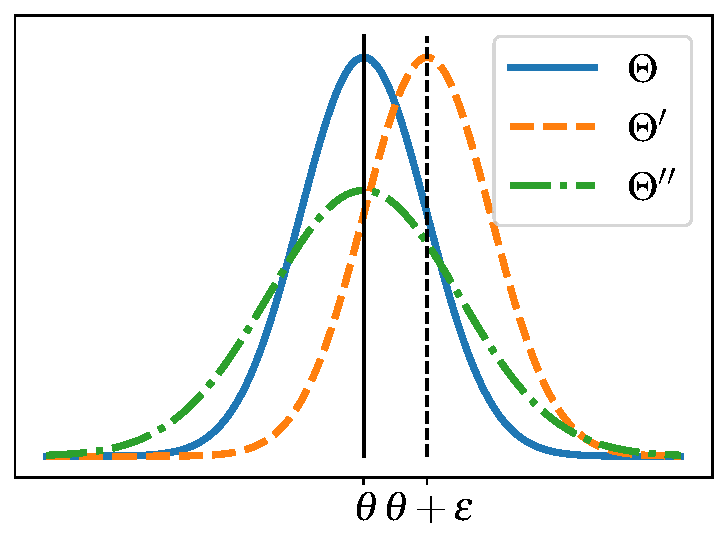
\includegraphics[width=0.5\textwidth]{figures/estimation/biais_variance}
  \caption{Distribution de 3 estimateurs de $\theta$.}
  \label{fig:biais_variance}
\end{figure}

\subsection{Exemple : Estimation non-biaisée de la variance}
\label{sec:unbiased_variance_estimation}
Considérons que $X$ est de carré intégrable ($X \in \Lcal^2$), d'espérance $\mu$ et
de variance $\sigma^2$.

La \textbf{variance empirique} de $X$ est une variable aléatoire $S_n$, définie
par
\begin{equation}
  S_n = \frac1n \sum_{i=1}^n (X_i - M_n)^2,
  \label{eq:variance_empirique}
\end{equation}
où $M_n$ est la moyenne empirique telle que définie précédemment.

$S_n$ est un estimateur de $\sigma^2.$

Cependant, son biais vaut $\frac{-1}{n} \sigma^2$  (voir calcul
  section~\ref{sec:biais_variance_empirique}).

On propose donc la \textbf{variance empirique corrigée,} définie par 
\begin{equation}
  S^*_n = \frac1{n-1} \sum_{i=1}^n (X_i - M_n)^2,
  \label{eq:variance_empirique_corrigee}
\end{equation}
et qui est non-biaisée.

Néanmoins, le biais de la variance empirique tend vers 0 lorsque $n$ tend vers
$+\infty$. On parle alors d'un estimateur \textbf{asymptotiquement non-biaisé.}

\subsection{Précision d'un estimateur}
\label{sec:precision_estimateur}

Reprenons la figure~\ref{fig:biais_variance}. Les deux estimateurs $\Theta$ et
$\Theta^{\prime\prime}$ sont non-biaisés. Cependant, $\Theta^{\prime\prime}$ a
une plus grande variance ; une de ses réalisation a une probabilité plus grande
que pour $\Theta$ d'être éloignée de $\theta$. Ainsi, $\Theta^{\prime\prime}$
est \textit{moins précis} que $\Theta.$
  
Un estimateur non-biaisé sera considéré d'autant plus précis que sa variance
est faible.  Dans le cas général d'un estimateur biaisé, il faut aussi prendre
en compte le biais dans la définition de la précision. Un estimateur biaisé
mais de variance faible pourra donner de meilleures estimations (c'est-à-dire
plus proches de la vraie valeur) qu'un estimateur moins biaisé mais avec une
plus grande variance.

C'est pourquoi on utilise pour quantifier la précision d'un estimateur ponctuel
générique son \textit{erreur quadratique moyenne,} définie comme
\begin{equation}
  \text{EQM}(\Theta_n) = \EE((\Theta_n - \theta)^2) = \VV(\Theta_n - \theta) + \EE((\Theta_n - \theta))^2
  = \VV(\Theta_n) + \text{B}(\Theta_n)^2.
  \label{eq:eqm}
\end{equation}
Un estimateur sera ainsi d'autant plus précis que son erreur quadratique moyenne est faible.

\paragraph{Compromis biais-variance} Il est tout à fait possible qu'un
estimateur biaisé ait une meilleure précision qu'un estimateur non-biaisé, si
ce dernier a une plus grande variance !

\begin{figure}[h]
  \centering
  \begin{subfigure}[t]{0.4\textwidth}
    \centering
    \begin{tikzpicture}
      \node[circle, minimum size=2, draw, fill=BrickRed] at (0, 0) {};
      \node[circle, minimum size=15, draw] at (0, 0) {};
      \node[circle, minimum size=25, draw] at (0, 0) {};
      \node[circle, minimum size=35, draw] at (0, 0) {};
      \node[circle, minimum size=45, draw] at (0, 0) {};
      \node[circle, minimum size=55, draw] at (0, 0) {};
      \node[circle, minimum size=65, draw] at (0, 0) {};

       \draw[fill=RoyalBlue] (0.4, 0.2) circle (2pt);
       \draw[fill=RoyalBlue] (-0.1, 0.3) circle (2pt);
       \draw[fill=RoyalBlue] (0.1, 0.2) circle (2pt);
       \draw[fill=RoyalBlue] (0.3, -0.1) circle (2pt);
       \draw[fill=RoyalBlue] (0.2, -0.2) circle (2pt);
       \draw[fill=RoyalBlue] (-0.4, 0.1) circle (2pt);
       \draw[fill=RoyalBlue] (0.1, 0.3) circle (2pt);
       \draw[fill=RoyalBlue] (0.3, 0.25) circle (2pt);
    \end{tikzpicture}     
    \caption{Biais faible, variance faible}
  \end{subfigure} \hfill
  \begin{subfigure}[t]{0.4\textwidth}
    \centering
    \begin{tikzpicture}
      \node[circle, minimum size=2, draw, fill=BrickRed] at (0, 0) {};
      \node[circle, minimum size=15, draw] at (0, 0) {};
      \node[circle, minimum size=25, draw] at (0, 0) {};
      \node[circle, minimum size=35, draw] at (0, 0) {};
      \node[circle, minimum size=45, draw] at (0, 0) {};
      \node[circle, minimum size=55, draw] at (0, 0) {};
      \node[circle, minimum size=65, draw] at (0, 0) {};

      \draw[fill=RoyalBlue] (0.6, 0.8) circle (2pt);
      \draw[fill=RoyalBlue] (-0.7, 0.65) circle (2pt);
      \draw[fill=RoyalBlue] (-0.4, -0.6) circle (2pt);
      \draw[fill=RoyalBlue] (0.5, -0.9) circle (2pt);
      \draw[fill=RoyalBlue] (0.7, -0.5) circle (2pt);
      \draw[fill=RoyalBlue] (-0.6, 0.2) circle (2pt);
      \draw[fill=RoyalBlue] (0.3, 0.2) circle (2pt);
      \draw[fill=RoyalBlue] (0.7, 0.5) circle (2pt);
    \end{tikzpicture}
    \caption{Biais faible, variance élevée}
  \end{subfigure}
  \begin{subfigure}[t]{0.4\textwidth}
    \centering
    \begin{tikzpicture}
      \node[circle, minimum size=2, draw, fill=BrickRed] at (0, 0) {};
      \node[circle, minimum size=15, draw] at (0, 0) {};
      \node[circle, minimum size=25, draw] at (0, 0) {};
      \node[circle, minimum size=35, draw] at (0, 0) {};
      \node[circle, minimum size=45, draw] at (0, 0) {};
      \node[circle, minimum size=55, draw] at (0, 0) {};
      \node[circle, minimum size=65, draw] at (0, 0) {};

      \draw[fill=RoyalBlue] (-0.7, -0.6) circle (2pt);
      \draw[fill=RoyalBlue] (-0.6, -0.5) circle (2pt);
      \draw[fill=RoyalBlue] (-0.75, -0.55) circle (2pt);
      \draw[fill=RoyalBlue] (-0.5, -0.7) circle (2pt);
      \draw[fill=RoyalBlue] (-0.4, -0.6) circle (2pt);
      \draw[fill=RoyalBlue] (-0.8, -0.7) circle (2pt);
      \draw[fill=RoyalBlue] (-0.7, -0.8) circle (2pt);
      \draw[fill=RoyalBlue] (-0.55, -0.5) circle (2pt);
     \end{tikzpicture}
    \caption{Biais élevé, variance faible}
  \end{subfigure} \hfill
  \begin{subfigure}[t]{0.4\textwidth}
    \centering
    \begin{tikzpicture}
      \node[circle, minimum size=2, draw, fill=BrickRed] at (0, 0) {};
      \node[circle, minimum size=15, draw] at (0, 0) {};
      \node[circle, minimum size=25, draw] at (0, 0) {};
      \node[circle, minimum size=35, draw] at (0, 0) {};
      \node[circle, minimum size=45, draw] at (0, 0) {};
      \node[circle, minimum size=55, draw] at (0, 0) {};
      \node[circle, minimum size=65, draw] at (0, 0) {};

      \draw[fill=RoyalBlue] (-0.2, -0.5) circle (2pt);
      \draw[fill=RoyalBlue] (-1., 0.3) circle (2pt);
      \draw[fill=RoyalBlue] (-0.1, -0.8) circle (2pt);
      \draw[fill=RoyalBlue] (-0.5, -0.9) circle (2pt);
      \draw[fill=RoyalBlue] (-0.9, -0.1) circle (2pt);
      \draw[fill=RoyalBlue] (-0.6, 0.2) circle (2pt);
      \draw[fill=RoyalBlue] (-0.3, -0.2) circle (2pt);
      \draw[fill=RoyalBlue] (-0.7, -0.5) circle (2pt);
    \end{tikzpicture}
    \caption{Biais élevé, variance élevée}
  \end{subfigure}
  \caption{Illustration des concepts de biais et de variance par analogie avec
    un jeu de fléchettes. La quantité à estimer est le centre de la cible ; les
    fléchettes sont les estimations. Chacune des sous-figures présente un
    estimateur différent.}
  \label{fig:flechettes}
\end{figure}


\subsection{Convergence d'un estimateur $\bullet$}
\label{sec:convergence_estimateur}
On souhaite aussi d'un estimateur qu'il permette de s'approcher d'autant mieux
de la quantité qu'il estime que la taille de l'échantillon est grande. On parle
ici de la convergence d'une série de variables aléatoires réelles,
$(\Theta_n)_{n \in \NN^*},$ vers une valeur réelle, $\theta$ ; il s'agit donc
en fait de considérer la convergence vers une variable aléatoire $\Theta$ qui
vaut $\theta$ presque partout.

On dit que l'estimateur $\Theta_n$ de $\theta$ \textbf{est convergent} s'il
converge en probabilité vers $\theta:$
\begin{equation}
  \label{eq:estimateur_convergent}
  (\Theta_n)_{n \in \NN^*} \cvproba \theta.
\end{equation}

Si de plus la convergence est presque sûre,
$(\Theta_n)_{n \in \NN^*} \cvps \theta,$ on dit alors que $\Theta_n$ est un
estimateur \textbf{fortement convergent} de $\theta$.

\paragraph{Proposition} Un estimateur sans biais et de variance
asymptotiquement nulle est convergent.

\paragraph{Preuve} La preuve en a été faite dans l'exercice « Convergence vers
une constante » de Probabilité IV. Pour rappel, posons $\Theta_n$ un estimateur
non biaisé et de variance asymptotiquement nulle de $\theta \in \RR$,
c'est-à-dire que $\EE(\Theta_n) = \theta$ et $\VV(\Theta_n) \cvn 0.$ $\Theta_n$
est donc d'espérance et de variance bornées et ainsi dans $\Lcal^2.$ Enfin,
$  \EE((\Theta_n - \theta)^2) = \VV(\Theta_n) + B(\Theta_n)^2,$
et donc $\EE((\Theta_n - \theta)^2) \cvn 0,$ ce qui signifie que
$\Theta_n \cvltwo \theta$ et donc $\Theta_n \cvproba \theta. \hfill \square$

\paragraph{Remarque} On utilise en anglais le terme de ``\textit{consistent}'',
ce qui conduit les francophones à parfois parler d'estimateur consistant plutôt
que convergent.

\subsection{Exercice (estimation de la moyenne)}
\label{sec:exo_proprietes}
Nous cherchons à déterminer le poids moyen à la naissance des bébés en
France. Pour cela, nous disposons d'un échantillon $(x_1, x_2, \dots, x_n)$ de
$n$ mesures obtenues dans plusieurs maternités à travers le pays.

Nous supposons que cet échantillon est une réalisation d'un échantillon
$(X_1, X_2, \dots, X_n)$ de variables aléatoire réelles indépendantes et
identiquement distribuées, d'espérance $m$ et de variance $\sigma^2$.

On propose deux estimateurs de $m$ : 
\[
  M_n = \frac1n \sum_{i=1}^n X_i \text{ et } Z_n = \frac12 (X_n + X_{n-1}).
\]

Montrer que $M_n$ et $Z_n$ sont sans biais. Lequel choisir pour approcher $m$ ?

(Solution : section~\ref{sec:sol_proprietes}.)


%-*- coding: utf-8 -*-
\section{QCM}

\paragraph{Question 1.} Soit $X$ une variable aléatoire réelle suivant une loi
de Poisson de paramètre $\lambda$. Étant donné un échantillon aléatoire
$(X_1, X_2, \dots, X_n)$ de $X$, et une de ses réalisations
$(x_1, x_2, \dots, x_n)$, cocher le(s) estimateur(s) non biaisé(s) de $\lambda$
parmi les propositions ci-dessous :
\begin{itemize}
\item[$\square$] $L_1 = \frac1n \sum_{i=1}^n x_i.$
\item[$\square$] $L_2 = \frac1n \sum_{i=1}^n X_i.$
\item[$\square$] $L_3 = \frac1n \sum_{i=1}^n \left( X_i^2 - \left( \frac1n \sum_{j=1}^n X_j \right)^2 \right).$
\item[$\square$] $L_4 = \frac1n \sum_{i=1}^n \left( x_i^2 - \left( \frac1n \sum_{j=1}^n x_j \right)^2 \right).$
\end{itemize}


\paragraph{Indice.}
{%
\noindent
\rotatebox[origin=c]{180}{%
\noindent
\begin{minipage}[t]{\linewidth}
Quelles sont l'espérance et la variance d'une loi de Poisson de paramètre $\lambda$ ?
\end{minipage}%
}%

\paragraph{Question 2.} Un estimateur biaisé peut être plus précis qu'un estimateur non-biaisé.
\begin{itemize}
\item[$\square$] Vrai.
\item[$\square$] Faux.
\end{itemize}


\section*{Solution}
{%
\noindent
\rotatebox[origin=c]{180}{%
\noindent
\begin{minipage}[t]{\linewidth}
\paragraph{Question 1.} Il y a ici tout d'abord une question de vocabulaire :
un estimateur est une variable aléatoire, tandis qu'une estimation est sa
réalisation. Ainsi nous ne considérons que les formules avec $X$ et non pas
avec $x$.

On rappelle que $\EE(X) = \lambda$ et $\VV(X) = \lambda.$

Seul $L_2$ est un estimateur sans biais de $\EE(X) = \lambda$ : c'est la moyenne
empirique de $X$.

On peut refaire le calcul : les $X_i$ étant i.i.d. de même loi que $X,$ 
\[
  \text{B}(L_2) = \EE(L_2) - \lambda = \frac1n \sum_{i=1}^n \EE(X_i) - \lambda = 0.
\]

$L_3$ est la variance empirique de $X$ et $L_3$ est donc un estimateur
biaisé de $\VV(X) = \lambda$. \newline

\paragraph{Question 2.} Vrai. C'est le concept du compromis biais-variance
(cf. section~\ref{sec:precision_estimateur}).
\end{minipage}%
}%

%%% Local Variables:
%%% mode: latex
%%% TeX-master: "../../sdd_2025_poly"
%%% End:




\section{Estimation par maximum de vraisemblance}
Nous considérons toujours dans cette section un échantillon aléatoire
$(X_1, X_2, \dots, X_n)$ de taille $n \in \NN^*$ d'une variable aléatoire
réelle $X$, et une quantité $\theta \in \Scal \subseteq \RR$ à estimer. Nous
notons $\PP_X$ la loi de $X$.

Nous venons de voir comment caractériser un estimateur $\Theta_n$ afin de
choisir le meilleur estimateur parmi plusieurs. Mais comment \textit{proposer} un
estimateur de $\theta$ ?

Supposons que $(x_1, x_2, \dots, x_n)$ est une réalisation de
$(X_1, X_2, \dots, X_n)$. La technique que nous allons voir consiste à
maximiser la vraisemblance de l'échantillon, autrement dit la probabilité
d'observer cet échantillon étant donnée la valeur estimée de $\theta$.

\begin{exemple}
  Nous nous intéressons à la réussite d'élèves au baccalauréat en
  \^Ile-de-France, et disposons d'observations issues de plusieurs lycées de la
  région.

  Nous modélisons l'observation \og réussite \fg~ou \og échec \fg~comme la
  réalisation d'une variable aléatoire $X$, de domaine $E = \{0, 1\}$ ($0$
  correspondant à \og échec \fg~et $1$ à \og réussite \fg), et suivant une loi
  de probabilité $\PP_X$.  Un choix classique pour cette loi de probabilité est
  d'utiliser une loi de Bernoulli de paramètre $p$:
  \[
    \PP_X(X=x) = p^x (1-p)^{1-x}.
  \] 
  Nos observations constituent un échantillon
  $(x_1, x_2, \dots, x_n)$, qui est une réalisation de l'échantillon aléatoire
  $(X_1, X_2, \dots, X_n)$ de composantes indépendantes et identiquement
  distribuées de même loi que $X$.

  Nous cherchons à estimer $p$ à partir de cet échantillon. 

  Supposons que notre échantillon contient $n=500$ élèves, dont $b=450$ ont
  eu le bac.

  La valeur $p=50\%$ est peu vraisemblable ; la valeur $p=90\%$ l'est beaucoup
  plus. C'est cette notion que nous allons formaliser par la suite.
\end{exemple}

La \textbf{vraisemblance} de l'échantillon $(x_1, x_2, \dots, x_n)$ quantifie à
quel point il est plausible d'observer cet échantillon en fonction de la valeur
de la quantité à estimer.

Pour tout $t \in \Scal$, nous notons $\PP_{n;t}$ la loi de l'échantillon aléatoire $(X_1,\dots,X_n)$ paramétrée par
$t.$ Supposons qu'il existe une mesure $\mu$ sur $(\RR^n, \Bcal(\RR^n))$ telle que
$\PP_{n;t}$ s'écrive sous la forme $\PP_{n;t}= f_{n;t} \mu,$ où
$f_{n;t}: \RR^n \mapsto \RR_+$ est $\mu$-mesurable. Dans le cas où l'échantillon aléatoire est à valeurs discrètes,
$\mu$ est la mesure de comptage et $f_{n;t}$ la fonction de masse (jointe) de $(X_1,\dots,X_n)$. Dans le
cas où il est à densité, $\mu$ est la mesure de Lebesgue et $f_{n;t}$ est la
densité (jointe) de $(X_1,\dots,X_n)$ (voir par exemple la section II.5 du chapitre « Espaces fonctionnels, théorie de la mesure
et de l'intégration »). La vraisemblance de $(x_1, x_2, \dots, x_n)$ est alors la
fonction de $t$ définie par
\begin{equation}
  L(x_1, x_2, \dots, x_n; t) = f_{n;t}(x_1,\dots,x_n).
  \label{eq:likelihood}
\end{equation}

En notant $\PP_{X;t}$ la loi de $X$ et $f_{t}$ sa densité ou fonction de masse, remarquez que la loi du $n$-échantillon aléatoire $(X_1, X_2, \dots, X_n)$ de $X$ est 
$  \PP_{n;t} = \PP_{X; t}^{\otimes n} $,
car les $X_i$ sont indépendantes et identiquement distribuées, et que la vraisemblance se simplifie :
$$L(x_1, x_2, \dots, x_n; t) = \prod_{i=1}^n f_{t}(x_i).$$

On appelle alors \textbf{estimation par maximum de vraisemblance} ({\it maximum
  likelihood estimate} ou {\it MLE} en anglais) de $\theta$ une valeur
$\hatmle{\theta}$ qui maximise la vraisemblance de l'échantillon
$(x_1, x_2, \dots, x_n)$:
\begin{equation}
  \label{eq:mle_estimator}
  \hatmle{\theta} \in \argmax_{t \in \Scal} \prod_{i=1}^n f_t(x_i).
\end{equation}

\textbf{Un estimateur par maximum de vraisemblance} de $\theta$ est une
variable aléatoire réelle $\hatmle{\Theta}$ dont la valeur quand
$X_1=x_1, X_2=x_2, \dots, X_n=x_n$ est donnée par $\hatmle{\theta}$.

Pour simplifier les calculs, on choisira souvent de maximiser non pas
directement la vraisemblance mais son logarithme :
\begin{equation}
  \label{eq:lmle_estimator} 
  \hatmle{\theta} \in \argmax_{t \in \Scal}\sum_{i=1}^n \ln f_t(x_i).
\end{equation}

\begin{exemple}
  Reprenons notre exemple de réussite au baccalauréat.
  
  L'estimation par maximum de vraisemblance de $p$ est
  \begin{align*}
    \hatmle{p} & = \argmax_{t \in [0, 1]} \sum_{i=1}^n \ln \PP_{X; t}(X=x_i)
                          = \argmax_{t \in [0, 1]} \sum_{i=1}^n \ln 
                          \left( t^{x_i} (1-t)^{1-x_i}  \right) \\
                        & = \argmax_{t \in [0, 1]} \sum_{i=1}^n x_i \ln t + 
                          \left( n - \sum_{i=1}^n x_i \right) \ln (1-t).
  \end{align*}
  La fonction que nous cherchons à minimiser est
  $\ell: t \mapsto \sum_{i=1}^n x_i \ln t + \left( n - \sum_{i=1}^n x_i \right)
  \ln (1-t).$

  Rappelons que l'on note $b = \sum_{i=1}^n x_i.$ Si $b=n$, alors
  $\ell(t) = n \ln t$ et $\ell$ est maximale quand $t=1.$

  Si $b=0$, alors $\ell(t) = n \ln (1-t)$ et $\ell$ est maximale quand $t=0.$

  Enfin, si $0 < b < n,$ la fonction que nous cherchons à minimiser est
  concave, nous pouvons donc la maximiser en annulant sa dérivée :
  \begin{equation*}
    \frac{d \ell}{d t} = \sum_{i=1}^n x_i \frac1t - 
    \left( n - \sum_{i=1}^n x_i \right) \frac1{1-t},
  \end{equation*}
  ce qui nous donne
  \begin{equation*}
    (1 - \hatmle{p}) \left( \sum_{i=1}^n x_i \right) - \hatmle{p} \left( n - 
      \sum_{i=1}^n x_i \right) = 0
  \end{equation*}
  et donc, pour toutes les valeurs possibles de $b,$
  \begin{equation}
    \label{eq:mle_bernoulli}
    \hatmle{p} = \frac{1}{n} \sum_{i=1}^n x_i = \frac{b}{n}.
  \end{equation}
  
  L'estimateur par maximum de vraisemblance de $p$ est ainsi tout simplement la
  moyenne empirique de l'échantillon. Dans notre exemple, $p=450/500=90\%.$
\end{exemple}


\paragraph{Propriété $\bullet$} L'estimateur par maximum de vraisemblance est
(sous des hypothèses généralement vérifiées) convergent. La démonstration,
plutôt pénible, repose sur l'application de la loi des grands nombres : le
paramètre maximisant la vraisemblance maximise aussi la log-vraisemblance ainsi
que la log-vraisemblance divisée par $n$.

\subsection{Exercice} 
\label{sec:rayleigh_exo}
Soit $X$ une variable aléatoire réelle dont la densité de probabilité est donnée par 
\[
  f(x; \sigma^2) = \frac{x}{\sigma^2} \exp \left( - \frac{x^2}{2 \sigma^2} \right) \text{ pour } x \in [0, +\infty[.
\]
On pourra vérifier\footnote{Par exemple sur \href{https://fr.wikipedia.org/wiki/Loi_de_Rayleigh}{https://fr.wikipedia.org/wiki/Loi\_de\_Rayleigh}.} qu'il s'agit d'une loi de Rayleigh de paramètre d'échelle
$\lambda = \sqrt{2} \sigma$. Ainsi son espérance et sa variance sont données par 
\[
  \EE(X) = \sqrt{\frac{\pi}{2}} \sigma \text{\qquad et \qquad} \VV(X) =
  \frac{4-\pi}{2} \sigma^2.
\]
Donner l'estimateur par maximum de vraisemblance de $\sigma^2$.
Solution : voir section~\ref{sec:rayleigh_sol}.


\section{Estimation de Bayes $\bullet$}
\label{sec:bayes_est}
Supposons que plutôt que de ne pas connaître du tout la valeur du paramètre
$\theta$, nous ayons une bonne idée des valeurs qu'il peut prendre. Cette
information peut être très utile, surtout quand le nombre d'observations est
faible.

Pour en tirer parti, nous allons utiliser une variable aléatoire réelle
$\Theta$ à valeurs dans $\Scal$, dont la loi $\PP_{\Theta}$ est la \textbf{loi
  a priori}, c'est-à-dire définie avant d'avoir observé un échantillon. Il va
maintenant s'agir d'utiliser la formule de Bayes pour exprimer la \textbf{loi a
  posteriori}, c'est-à-dire conditionnellement à un échantillon aléatoire, de
$\Theta$.

Si $\Theta$ est discrète, la formule de Bayes nous permet
d'écrire la loi de $\Theta|X_1, X_2, \dots, X_n :$
\begin{equation}
  \label{eq:bayes_discret}
  \PP_{\Theta|X_1, X_2, \dots, X_n}(\Theta=t) = \frac{\PP_{\Theta}(t) \prod_{i=1}^n f_t(x_i)}{
    \sum_{u \in \Scal} \PP_{\Theta}(u) \prod_{i=1}^n f_u(x_i)}
\end{equation}

Si $\Theta$ est à densité, de densité $g_{\Theta},$ alors
$\Theta|X_1, X_2, \dots, X_n$ est aussi à densité et la formule de Bayes nous
permet d'écrire sa densité comme : 
\begin{equation}
  \label{eq:bayes_densite}
  g_{\Theta|X_1, X_2, \dots, X_n}(t) = \frac{g_{\Theta}(t) \prod_{i=1}^n f_t(x_i)}{
    \int_{\Scal} g_{\Theta}(u) \prod_{i=1}^n f_u(x_i) du}
\end{equation}
Ces manipulations de Bayes sont analogues à celles effectuées dans le poly de
Probabilités III, en particulier dans la section « Formule de balayage
conditionnel » et dans l'exercice « Loi conjuguées ».

En d'autres termes, l'observation d'un échantillon permet d'ajuster la loi a
priori de $\Theta$ en sa loi a posteriori. Cette idée est au c\oe{}ur
de \textbf{l'inférence bayésienne.}

\subsection{Estimation par maximum a posteriori}

L'\textit{estimation par maximum a posteriori} de $\theta$ est définie comme
une valeur de $\Scal$ qui maximise la loi a posteriori de $\Theta$. Ainsi dans
le cas discret,
\begin{equation}
  \label{eq:map_discret}
  \hatmap{\theta} \in \argmax_{t \in \Scal} \PP_{\Theta|X_1, X_2, \dots, X_n}(\Theta=t)
\end{equation}
et dans le cas à densité,
\begin{equation}
  \label{eq:map_densite}
  \hatmap{\theta} \in \argmax_{t \in \Scal} g_{\Theta|X_1, X_2, \dots, X_n}(t).
\end{equation}
   
L'estimateur par maximum a posteriori coincide avec l'estimateur par
maximum de vraisemblance si la distribution a priori utilisée est une
distribution uniforme.
  

\subsection{Estimation de Bayes}
L'estimation par maximum a posteriori est limitée dans le cas où la
distribution a posteriori est multi-modale ; en effet, le mode le plus grand
peut être difficile à identifier par des algorithmes de gradient. De plus, elle
ne prend en compte qu'un seul point de la distribution a posteriori, plutôt que
de la considérer dans son intégralité.

L'estimation de Bayes de $\theta$ est définie comme une valeur de $\Scal$ qui
% est la mieux estimée par la loi a posteriori de $\Theta$
minimise en espérance une fonction de coût sur la loi a posteriori de $\Theta$.
Cette définition est
générale, et dépend de la fonction de coût utilisée. %du sens donné à « mieux estimée par » ;
Nous utiliserons
une des définitions les plus courantes, et considérerons à partir de maintenant
l'erreur quadratique moyenne (définie section~\ref{sec:precision_estimateur}). 

L'\textbf{estimation de Bayes pour l'erreur quadratique moyenne} de $\theta$
est ainsi définie par
\begin{equation}
  \label{eq:bayes_estimator}
  \hatbys{\theta} \in \argmin_{t \in \Scal} \EE([(\Theta|X_1=x_1, X_2=x_2, \dots, X_n=x_n) - t)]^2).
\end{equation}


\paragraph{Propriété} L'estimation de Bayes pour l'erreur quadratique moyenne
est l'espérance de la distribution a posteriori de $\Theta$ : 
\begin{equation}
  \label{eq:bayes_estimator2}
  \hatbys{\theta}  = \EE(\Theta|X_1 = x_1, X_2=x_2, \dots, X_n=x_n).
\end{equation}

\paragraph{Preuve}
En effet, posons $t \in \Scal.$ Notons
$W = (\Theta|X_1=x_1, X_2=x_2, \dots, X_n=x_n)$ pour simplifier l'écriture.
Alors
\begin{equation*}
  \EE((W - t)^2) =  \EE(W^2) + t^2 - 2 t \EE(W) =  \EE(W^2) + [\EE(W) - t]^2 - \EE(W)^2.  
\end{equation*}
Comme ni $\EE(W^2)$ ni $\EE(W)^2$ ne dépendent de $t,$
$\hatbys{\theta}$ est obtenue en minimisant $(\EE(W) - t)^2$ et donc $\hatbys{\theta} = 
\EE(W). \hfill \square$

\begin{exemple}
  Reprenons notre exemple de taux de réussite au baccalauréat.  Nous supposons
  maintenant que $p$ est une réalisation d'une variable aléatoire $\Theta$ qui
  suit une loi bêta de paramètres $(\alpha, \beta)$
  (cf. section~\ref{sec:loi_beta}) et dont nous notons $g_\Theta$ la densité.

  Pour calculer l'estimateur de Bayes de $p$, il nous faut connaître la loi de
  $(\Theta|X_1=x_1, X_2=x_2, \dots, X_n=x_n)$. $\Theta$ étant à densité,
  $(\Theta|X_1=x_1, X_2=x_2, \dots, X_n=x_n)$ aussi et la loi de Bayes,
  combinée à l'hypothèse d'indépendance et de distribution identique des $X_i$,
  nous permet d'écrire sa densité comme 
  \begin{flalign*}
     & g_{\Theta|X_1=x_1, \dots, X_n=x_n}(t)  = \frac{\PP(X_1=x_1, \dots, X_n=x_n|\Theta=t) g_\Theta(t)}{\PP(X_1=x_1, \dots, X_n=x_n)} \\
    & = \frac{1}{\PP(X_1=x_1, \dots, X_n=x_n) B(\alpha, \beta)} 
    \prod_{i=1}^{n} t^{x_i} (1-t)^{1-x_i} t^{\alpha-1}
    (1-t)^{\beta-1} \\
    & = \frac{1}{\PP(X_1=x_1, \dots, X_n=x_n) B(\alpha, \beta)} 
    t^{b + \alpha - 1} (1-t)^{n - b + \beta - 1}. 
  \end{flalign*}
  
  On reconnaît ici la densité d'une nouvelle loi bêta.  Ainsi
  $(\Theta|X_1=x_1, \dots, X_n=x_n)$ suit une loi bêta de paramètres $(b + \alpha)$ et
  $(n - b + \beta).$

  L'estimation de Bayes de $p$ est ainsi
  \begin{equation*}
    \hatbys{p} = \EE(\Theta|X_1=x_1, X_2=x_2, \dots, X_n=x_n) = \frac{(b + \alpha)}{
      (b + \alpha) + (n - b + \beta)}
    = \frac{b + \alpha}{n + \alpha + \beta}.
  \end{equation*}
  Cette première égalité est obtenue d'après la formule donnant l'espérance
  d'une loi bêta (cf section~\ref{sec:loi_beta}).

  \textbf{Remarque importante}
  On peut réécrire cette estimation sous la forme
  \begin{equation*}
    \hatbys{p} = \frac{\alpha + \beta}{n + \alpha + \beta} \EE[\Theta] + 
    \frac{n}{n + \alpha + \beta} \hatmle{p}.
  \end{equation*}
  Ainsi, l'estimation de Bayes du paramètre $p$ est une combinaison linéaire de
  l'espérance de sa distribution a priori et de son estimation par maximum de
  vraisemblance.

  De plus, le coefficient multiplicatif de l'espérance a priori décroît en
  fonction de la taille $n$ de l'échantillon, tandis que le coefficient
  multiplicatif de l'estimation par maximum de vraisemblance croît en fonction
  de $n$. Ainsi, plus l'échantillon est grand, plus l'estimateur de Bayes fait
  confiance aux données, et s'éloigne de l'espérance a priori du paramètre,
  dont on est plus proche avec un petit échantillon.

  La figure~\ref{fig:bayes_estimate} illustre cet exemple.

  \textbf{Remarque} Le choix d'une loi bêta ne s'est pas fait au hasard. On
  retrouve ici les lois conjuguées présentées en exercice de Probabilités
  III. En inférence bayésienne, on dit qu'une loi a priori et une loi a
  posteriori sont conjuguées lorsqu'elles appartiennent à la même famille. En
  particulier, la loi bêta est conjuguée à elle-même pour une vraisemblance de
  Bernoulli.
\end{exemple}

\begin{figure}[h]
  \centering
  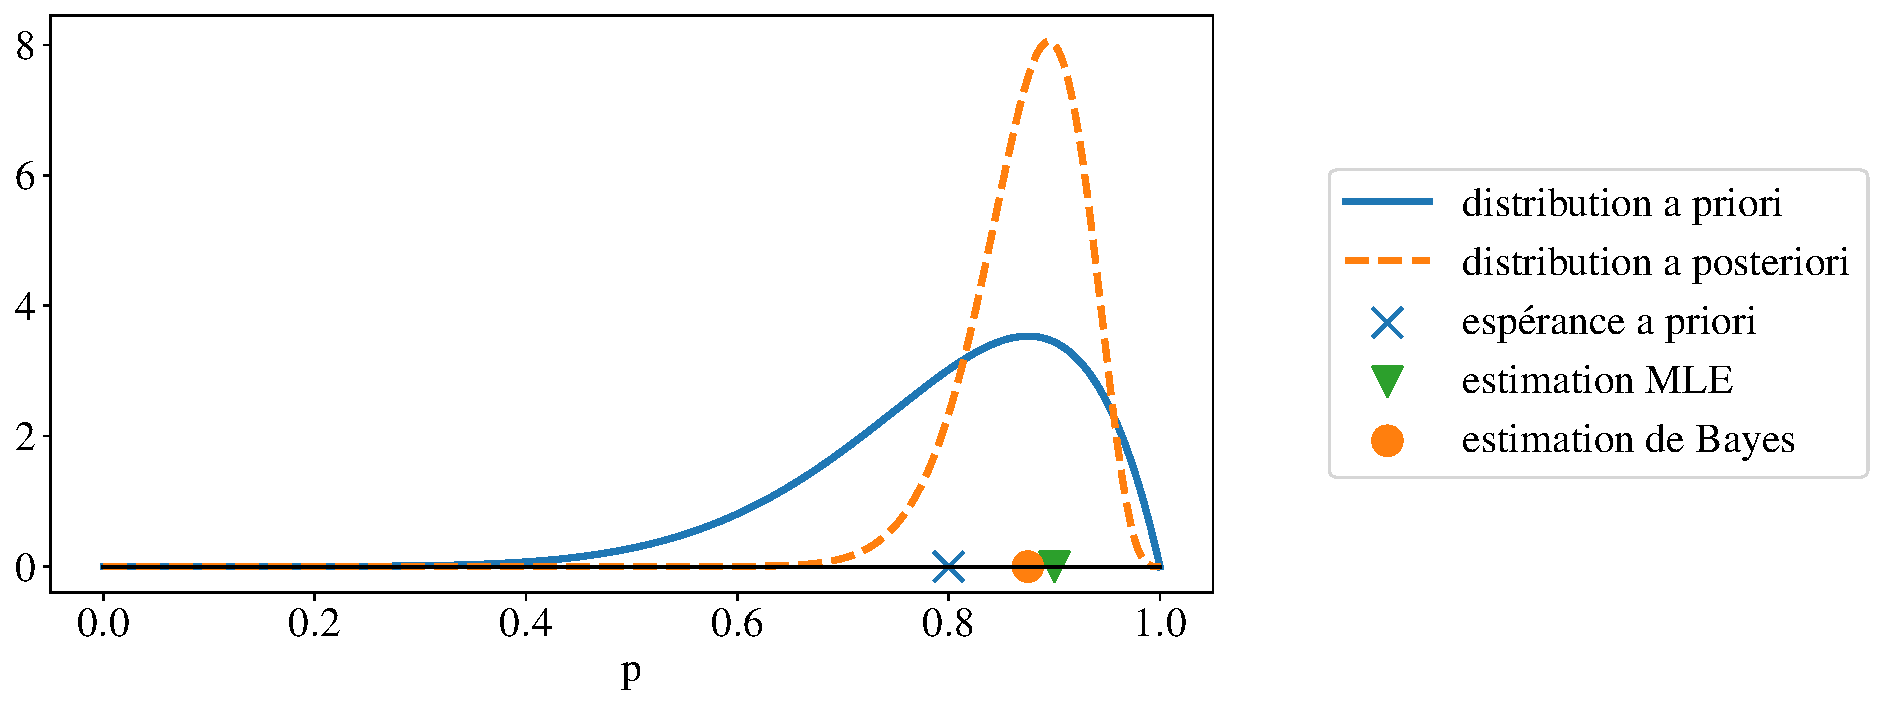
\includegraphics[width=\textwidth]{figures/estimation/bayes_estimate}
  \caption{Loi a priori et a posteriori pour le paramètre $p$ dans l'exemple du
    taux de réussite au baccalauréat. Sans voir de données, $p=0,80$,
    c'est-à-dire l'espérance de sa loi a priori (croix bleue). En utilisant
    uniquement l'échantillon, $p=0,90$, c'est-à-dire son estimation par maximum
    de vraisemblance (triangle vert). L'estimation de Bayes (rond orange) est
    intermédiaire.}
  \label{fig:bayes_estimate}
\end{figure}




\section{Compléments}
\subsection{Variance de la moyenne empirique} 
\label{sec:variance_moyenne_empirique}

Soit $X$ une variable aléatoire
réelle de carré intégrable, d'espérance $m$ et de variance $\sigma^2$. Soient
$X_1, X_2, \dots, X_n$ indépendantes et identiquement distribuées, de même loi
que $X$. 

Par définition de la variance, $\sigma^2 = \EE(X^2) - \EE(X)^2$ donc
$\EE(X^2) = \sigma^2 + m^2$.

Posons $M_n = \frac1n \sum_{i=1}^n X_i.$
\begin{align*}
  \VV(M_n) &= \EE(M_n^2) - \EE(M_n)^2 
   = \EE\left(\left(\frac1n \sum_{i=1}^n X_i\right)^2\right) - m^2 
   = \frac1{n^2} \EE\left( \sum_{i=1}^n X_i \sum_{j=1}^n X_j\right) - m^2 \\
  & = \frac1{n^2} \EE\left( \sum_{i=1}^n \left(X_i^2 + \sum_{j \neq i }^n X_i X_j \right) \right) - m^2 
   = \frac1{n} \left(\EE(X^2) + \sum_{j \neq i }^n \EE(X)^2 \right) - m^2, 
\end{align*}
par linéarité de l'espérance et car, pour $i \neq j$, $X_i$ et $X_j$ sont indépendantes et donc $\EE(X_iX_j) = \EE(X_i) \EE(X_j) = \EE(X)^2.$
Ainsi,
\[
  \VV(M_n) = \frac1{n} \left(\underbrace{\sigma^2 + m^2}_{\EE(X^2)} + (n-1) \, \underbrace{m^2}_{\EE(X)^2}  \right) - m^2 = \frac{\sigma^2}{n}.
\]

\subsection{Biais de la variance empirique} 
\label{sec:biais_variance_empirique}
Soit $X$ une variable aléatoire
réelle de carré intégrable, d'espérance $m$ et de variance $\sigma^2$. Soient
$X_1, X_2, \dots, X_n$ indépendantes et identiquement distribuées, de même loi
que $X$. 

Posons $M_n = \frac1n \sum_{i=1}^n X_i$ et $S_n = \frac1n \sum_{i=1}^n (X_i - M_n)^2.$ Alors
\begin{align*}
  \EE(S_n) = \frac1n \sum_{i=1}^n \EE((X_i - M_n)^2)  & =  
    \frac1n \sum_{i=1}^n \left( \EE(X_i^2) +  \EE(M_n^2) - 2 \EE(X_i M_n) \right)  \\
  & = \EE(X^2) + \EE(M_n^2) - \frac2n \sum_{i=1}^n \EE(X_i M_n).
\end{align*}
Nous avons montré lors du calcul de la variance de la moyenne empirique (section~\ref{sec:variance_moyenne_empirique}) que
$\EE(X^2) = \sigma^2 + m^2$ et que $\EE(M_n^2) = m^2 + \frac{\sigma^2}{n}.$
De plus, par linéarité de l'espérance,
\[
  \EE(M_n^2) = \EE\left( \left(\frac1n \sum_{i=1}^n X_i \right) M_n \right) = \frac1n \sum_{i=1}^n \EE(X_i M_n),
\]
et donc 
\[
  \EE(M_n^2) - \frac2n \sum_{i=1}^n \EE(X_i M_n) = - \EE(M_n^2).
\]

On obtient ainsi 
\[
  \EE(S_n) = (\sigma^2 + m^2) - \left(m^2 + \frac{\sigma^2}{n}\right) = \frac{n-1}{n} \sigma^2.
\]
La variance empirique est donc biaisée et son biais vaut 
\[
  \text{B}(S_n) = \EE(S_n) - \sigma^2 = - \frac1n \sigma^2.
\]

\subsection{Solution de l'exercice~\ref{sec:exo_proprietes}}
\label{sec:sol_proprietes}
La démonstration pour la moyenne empirique $M_n$ a été faite plus haut.

En ce qui concerne $Z_n$, 
\[
  \EE(Z_n) = \frac12 (\EE(X_n) + \EE(X_{n-1})) = m.
\]

Nous avons assez naturellement envie d'utiliser $M_n$, qui utilise toutes les
observations, plutôt que $Z_n$, qui n'en utilise que deux.

Pour nous en convaincre, nous pouvons comparer les variances de $M_n$ et
$Z_n$. La variance de la moyenne empirique est $\VV(M_n) = \frac{\sigma^2}{n}$
(voir plus haut). La variance de $Z_n$, elle, vaut
\[
  \VV(Z_n) = \frac14 \left( \VV(X_n) + \VV(X_{n-1}) \right) = \frac{\sigma^2}{2},
\]
la première égalité étant obtenue par indépendance de $X_n$ et $X_{n-1}$.

$Z_n$ est ainsi un estimateur bien moins précis que $M_n$ dès que $n>2.$

\subsection{Loi Beta}
\label{sec:loi_beta}
La densité de probabilité de la {\it loi bêta} de paramètres
$\alpha, \beta > 0$, définie sur $0 \leq u \leq 1$, est donnée par :
\begin{equation}
  \label{eq:beta_distribution}
  f_{\alpha, \beta} (u) = \frac{u^{\alpha -1} (1-u)^{\beta-1}}{B(\alpha, \beta)}     
\end{equation}
où
$B(\alpha, \beta) = \frac{\Gamma(\alpha) \Gamma(\beta)}{\Gamma(\alpha+\beta)}$
et $\Gamma$ est la fonction gamma. L'espérance de cette loi est
$\frac{\alpha}{\alpha + \beta}$.

\subsection{Solution de l'exercice~\ref{sec:rayleigh_exo}}
\label{sec:rayleigh_sol}
Soit $(x_1, x_2, \dots, x_n)$ un échantillon de $X$ de taille $n \in \NN^*.$ La
log-vraisemblance de l'échantillon est donnée par
\[
  \ell(x_1, x_2, \dots, x_n; \sigma^2) = \sum_{i=1}^n \ln \left(
    \frac{1}{\sigma^2} x_i \exp\left(- \frac{x_i^2}{2\sigma^2} \right)\right) 
  = -n \ln(\sigma^2) + \sum_{i=1}^n \ln(x_i) - \frac{1}{2\sigma^2} \sum_{i=1}^n x_i^2.
\]
Ainsi, l'estimation par maximum de vraisemblance de $\sigma^2$ est donnée par :
\[
  \hatmle{\sigma^2} \in \argmax_{s \in \RR_+} \left(-n \ln(s) + \sum_{i=1}^n \ln(x_i) - 
\frac{1}{2s} \sum_{i=1}^n x_i^2\right).
\]
On obtient un point critique de la fonction de $\RR_+$ dans $\RR$ qui à $s$
associe $-n \ln(s) + \sum_{i=1}^n \ln(x_i) - \frac{1}{2s} \sum_{i=1}^n x_i^2$
en annulant sa dérivée, qui vaut :
\[
  s \mapsto - \frac{n}{s} + \frac12 \sum_{i=1}^n x_i^2 \frac{1}{s^2},
\]
et donc 
\[
  \hatmle{\sigma^2} = \frac{1}{2n} \sum_{i=1}^n x_i^2.
\]
(On vérifiera que ce point critique est bien un maximum.)
Ainsi, étant donné un échantillon aléatoire $(X_1, X_2, \dots, X_n)$ de $X$,
l'estimateur par maximum de vraisemblance de $\sigma^2$ est donné par
\[
  S_n = \frac{1}{2n} \sum_{i=1}^n X_i^2.
\]


\begin{plusloin}
\item Un exercice sur la fonction de répartition empirique vous a été proposé
  dans le poly de Probabilité III.
\item On peut construire un estimateur par la \textit{méthode des moments}, qui
  consiste à faire coincider les moments théoriques de $\PP_X$ (qui dépendent
  donc de $\theta$) avec les moments empiriques de l'échantillon. La loi des
  grands nombres justifie en effet d'approcher la moyenne par la moyenne
  empirique. Cette méthode est généralement moins précise que le maximum de
  vraisemblance.
\item Plus la variance d'un estimateur est faible, plus cet estimateur
  peut-être considéré comme précis. La \textit{borne de Cramér-Rao} est une
  borne inférieure de cette variance pour un estimateur sans biais, en se
  basant sur l'information de Fisher. On dit qu'un estimateur est
  \textit{efficace} s'il est non-biaisé et que sa variance tend vers sa borne
  de Cramér-Rao.
\end{plusloin}

%\clearpage
%-*- coding: utf-8 -*-

\section{QCM}
\paragraph{Question 1.} Soit $(x_1, x_2, \dots, x_n)$ un échantillon d'une
variable aléatoire $X$ discrète. On suppose que $X$ suit une loi paramétrisée
par $\gamma$. La vraisemblance de $(x_1, x_2, \dots, x_n)$ est donnée par
\begin{itemize}
\item[$\square$] $\PP(X=x_1, X=x_2, \dots, X=x_n, \gamma)$
\item[$\square$] $\PP(X=x_1, X=x_2, \dots, X=x_n | \gamma)$
\item[$\square$] $\PP(\gamma | X=x_1, X=x_2, \dots, X=x_n)$
\item[$\square$] $\prod_{i=1}^n \PP(X=x_i|\gamma)$
\item[$\square$] $\prod_{i=1}^n \PP(\gamma|X=x_i)$
\end{itemize}

\paragraph{Question 2.} Soit $X$ une loi exponentielle de paramètre
$\lambda$. L'estimateur par maximum de vraisemblance de $\lambda$ est donné par
\begin{itemize}
\item[$\square$] $L_n = n \ln(\lambda) - \lambda \sum_{i=1}^n X_i,$ où $(X_1, X_2, \dots, X_n)$ est un échantillon aléatoire de $X$
\item[$\square$] $\widehat{\lambda} = n \ln(\lambda) - \lambda \sum_{i=1}^n x_i,$ où $(x_1, x_2, \dots, x_n)$ est un échantillon aléatoire de $X$
\item[$\square$] $L_n = \frac{n}{\sum_{i=1}^n X_i},$ où $(X_1, X_2, \dots, X_n)$ est un échantillon aléatoire de $X$
\item[$\square$] $\widehat{\lambda} = \frac{n}{\sum_{i=1}^n x_i},$ où $(x_1, x_2, \dots, x_n)$ est un échantillon aléatoire de $X$.
\end{itemize}

\paragraph{Question 3. $\bullet$} L'estimateur de Bayes est plus proche de l'espérance a
priori que de l'estimateur par maximum de vraisemblance quand la taille de
l'échantillon est
\begin{itemize}
\item[$\square$] grande
\item[$\square$] petite
\item[$\square$] ça dépend.
\end{itemize}



\section*{Solution}

{%
\noindent
\rotatebox[origin=c]{180}{%
\noindent
\begin{minipage}[t]{\linewidth}
\paragraph{Question 1.} Par définition (cf. équation~\ref{eq:likelihood}),
\[
L(x_1, x_2, \dots, x_n; \gamma) = \PP(x_1, x_2, \dots, x_n | \gamma) = \prod_{i=1}^n \PP(x_i|\gamma).
\]

\paragraph{Question 2.} 
Par définition la vraisemblance d'un échantillon $(x_1, x_2, \dots, x_n)$ est donnée par
\[
  L(x_1, x_2, \dots, x_n; \lambda) = \prod_{i=1}^n \lambda e^{- \lambda x_i}
  = \lambda^n \prod_{i=1}^n e^{- \lambda x_i},
\] 
et donc sa \textit{log-vraisemblance} vaut 
\[
  \ell(x_1, x_2, \dots, x_n; \lambda) = \ln \left(\lambda^n \prod_{i=1}^n e^{- \lambda x_i}\right)
  = n \ln(\lambda) - \lambda \sum_{i=1}^n x_i.
\]
La fonction $\lambda \mapsto n \ln(\lambda) - \lambda \sum_{i=1}^n x_i$ est
concave sur $]0, +\infty[ \rightarrow \RR$ et on peut donc la maximiser en
annulant sa dérivée.

On obtient \textit{l'estimation par maximum de vraisemblance} de $\lambda$ suivante :
\[
  \hatmle{\lambda} = \frac{n}{\sum_{i=1}^n x_i}
\]
et, si on appelle $(X_1, X_2, \dots, X_n)$ un échantillon aléatoire de $X$, on
obtient \textit{l'estimateur par maximum de vraisemblance} de $\lambda$ :
\[
  L_n = \frac{n}{\sum_{i=1}^n X_n}.
\]


\paragraph{Question 3.} La tendance que nous avons observée sur l'exemple de la
section~\ref{sec:bayes_est} (cf. « Remarque importante ») se vérifie en général : plus on
observe d'échantillons, plus on s'éloigne de l'a priori pour se rapprocher d'un
estimateur issu uniquement des données.
\end{minipage}%
}%

%%% Local Variables:
%%% mode: latex
%%% TeX-master: "../../sdd_2025_poly"
%%% End:




%%% Local Variables:
%%% mode: latex
%%% TeX-master: "../sdd_2025_poly"
%%% End:



\clearpage

\chapter{Tests d'hypothèse}
%-*- coding: utf-8 -*-
\label{chap:tests}

\paragraph{Notions :} hypothèse nulle, hypothèse alternative, statistique de
test, p-valeur, tests multiples.
\paragraph{Objectifs pédagogiques :} 
\begin{itemize}      
	\setlength{\itemsep}{3pt}
	\item Reconnaître une situation dans laquelle un test statistique est
	approprié.
	\item Poser les hypothèses de test nulle et alternative correspondant à un
	énoncé.
	\item Interpréter une statistique de test ou une p-valeur.
\end{itemize}


\section{Principe d'un test statistique}
\label{sec:principe_test}
Le but d'un test statistique est de déterminer la fiabilité d'un résultat
obtenu sur un échantillon.

\begin{exemple}
	Si je lance une pièce 5 fois et obtiens 5 fois pile, puis-je en déduire que
	la pièce est déséquilibrée ? Ou ce résultat est-il dû au hasard de
	l'échantillonnage ? Qu'en est-il si j'obtiens le même résultat après 50
	lancers ? 
\end{exemple}

\textbf{Un test statistique permet de déterminer si l'échantillon observé
	permet d'invalider une hypothèse qu'il était raisonnable de formuler avant
	d'observer les données.}

\begin{exemple}
	Reprenons l'exemple du lancer de pièce. Sous l'hypothèse que la pièce est
	équilibrée, la probabilité $\pi$ d'obtenir « pile » pour un lancer est $0,5$
	et celle d'obtenir pile pour 5 lancers est $0,5^5 = 3\%.$ Cette probabilité
	est faible, mais non négligeable : on a 3\% de chance d'obtenir un résultat
	aussi extrême que celui observé sur un échantillon.
	
	Pour 50 lancers, cette probabilité tombe à $0,5^{50} = 9 \cdot 10^{-16}.$
	Cette probabilité est extrêmement faible, et l'échantillon n'est pas cohérent
	avec l'hypothèse selon laquelle la pièce est équilibrée. Il est raisonnable
	de la rejeter.
\end{exemple}

\section{Formalisme}
\label{sec:formalisme_test}
Soit $(X_1, X_2, \dots, X_n)$ un échantillon aléatoire de taille $n \in \NN^*$
d'une variable aléatoire réelle $X$ de loi $\PP_X.$ Rappelons que les
composantes $X_i$ de ce vecteur aléatoire sont indépendantes et identiquement
distribuées, de même loi que $X$. Les notions présentées dans ce chapitre
s'appliquent aussi à des variables aléatoires de nature plus complexe (par
exemple, des valeurs aléatoires multi-dimensionnelles) mais nous nous limitons
aux variables aléatoires réelles par souci de simplicité.
Nous supposons aussi disposer d'un échantillon $(x_1, x_2, \dots, x_n)$ qui est
une réalisation de $(X_1, X_2, \dots, X_n)$.

Un test statistique repose sur les éléments suivants :
\begin{itemize}
	\item Une \textbf{hypothèse nulle,} notée $\HH_0$. L'hypothèse nulle est
	celle que l'on cherche à rejeter.
	\item Une \textbf{hypothèse alternative,} notée $\HH_1$ ou $\HH_a$. C'est en
	général la négation de $\HH_0$.
	\item Une \textbf{statistique de test,} $T$, qui sert à mesurer à quel point un
	échantillon « dévie » de l'hypothèse nulle.
	\item Un \textbf{niveau de signification,} $0 < \alpha < 1$, qui est la
	probabilité de rejeter l'hypothèse nulle alors qu'elle est correcte. 
	% qui sert à
	% déterminer si la probabilité d'observer, sous $\HH_0$, une statistique de
	% test au moins aussi extrême que celle observée sur l'échantillon
	% $(x_1, x_2, \dots, x_n)$ est suffisamment faible pour rejeter $\HH_0$.
\end{itemize}

Le but de cette section est de développer ces notions.

\subsection{Hypothèses de test}
Conduire un test d'hypothèse nécessite de formuler deux hypothèses :
\begin{itemize}
	\item Une \textbf{hypothèse nulle,} notée $\HH_0$. Cette hypothèse doit être
	précise et permettre de faire des calculs. Le but du test est de déterminer
	s'il est raisonnable de rejeter cette hypothèse.
	\item Une \textbf{hypothèse alternative,} notée $\HH_1$ ou $\HH_a$. Cette
	hypothèse est une forme de négation de $\HH_0$, et c'est l'hypothèse que l'on
	adoptera si l'hypothèse nulle est rejetée.
\end{itemize}

L'hypothèse nulle est souvent une hypothèse formulée sur la valeur d'un paramètre
$\theta \in \Scal \subseteq \RR$ caractérisant la loi $\PP_X$ de l'échantillon
aléatoire. Il s'agit alors de tester
\begin{equation}
	\label{eq:h0}
	\HH_0: \theta = \theta_0,
\end{equation}
où $\theta_0 \in \Scal$ est une valeur déterministe fixée à l'avance.

L'hypothèse nulle peut cependant être de nature plus complexe, par exemple :
\begin{itemize}
	\item « Deux variables statistique $X$ et $Y$ sont indépendantes » (c'est le
	cas du test d'indépendance du $\chi^2$ que nous verrons dans la PC2);
	\item « Deux échantillons $(x_1, x_2, \dots, x_n)$ et $(y_1, y_2, \dots, y_n)$
	sont des réalisations de la même distribution » (c'est le cas du test de
	Wilcoxon-Mann-Whitney, qui dépasse le cadre de ce programme).
\end{itemize}

\paragraph{Présomption d'innocence} De même que le principe de la présomption
d'innocence veut que l'on recueille suffisamment de preuves pour rejeter
l'innocence d'une personne accusée, en théorie des tests statistiques il y a
présomption de $\HH_0$. Il s'agit donc de savoir si l'échantillon observé (les
preuves) est suffisant pour rejeter $\HH_0$, ce dont on conclura $\HH_1.$ Par
contre, si l'on ne rejette pas $\HH_0$, cela peut venir soit de ce que $\HH_0$
est vraie, soit de ce que nous n'avons pas suffisamment de données pour rejeter
$\HH_0$. Ainsi, $\HH_0$ doit être une hypothèse raisonnable, mais que l'on
aimerait avoir des raisons de réfuter.

Dans le cadre d'une expérience scientifique, l'hypothèse $\HH_0$ correspond
ainsi à l'état actuel des connaissances. Le but d'un test statistique est de
déterminer si les données qui semblent contredire cette hypothèse sont
effectivement suffisamment improbables sous $\HH_0$ pour justifier de la
réfuter.
Dans le cadre d'un essai clinique, par exemple, l'hypothèse $\HH_0$ se doit
d'être défavorable au nouveau médicament (« le nouveau médicament est
inefficace » ou « le nouveau médicament n'est pas plus efficace que les
traitements connus »). Le but du test statistique est de déterminer si les
données récoltées jusqu'à présent sont suffisantes pour réfuter cette
hypothèse.

\begin{exemple}
	Dans le cas de notre lancer de pièce,
	\begin{itemize}
		\item $X$ est une variable aléatoire discrète qui suit une loi de Bernoulli
		de paramètre $\pi$ ;
		\item l'échantillon aléatoire est un vecteur $(X_1, X_2, \dots, X_n)$ de $n$
		composantes, iid de même loi que $X$ ;
		\item une série de lancers est une réalisation $(x_1, x_2, \dots, x_n)$ de ce
		vecteur aléatoire. Dans le cas de 5 lancers tous tombant sur « pile »,
		cet échantillon est $(1, 1, 1, 1, 1)$ et $n=5.$
		\item l'hypothèse nulle est $\HH_0: \pi = 0,5.$
	\end{itemize}
\end{exemple}

Dans le cas où l'on cherche à tester la valeur d'un paramètre $\theta$ d'une
population, l'hypothèse alternative peut prendre deux formes :
\begin{itemize}
	\item $\theta \neq \theta_0$, ou en d'autres termes, 
	\begin{equation}
		\label{eq:h1_bilateral}
		\HH_1: \theta < \theta_0 \text{ ou } \theta > \theta_0.
	\end{equation}
	On parle alors de test \textbf{bilatéral} (\textit{two-sided test} en
	anglais).
	\item Si seulement l'une des deux parties de cette hypothèse alternative nous
	intéresse, ou est possible, on parle de test \textbf{unilatéral}
	(\textit{one-sided test} en anglais). Il s'agit alors de tester soit
	\begin{equation}
		\label{eq:h1_unilateral_gauche}
		\HH_1: \theta < \theta_0,
	\end{equation}
	soit
	\begin{equation}
		\label{eq:h1_unilateral_droite}
		\HH_1:  \theta > \theta_0.
	\end{equation}
\end{itemize}

De même que l'on élabore $\HH_0$ de sorte à ce qu'elle soit la plus plausible
avant d'avoir observé les données, on élabore $\HH_1$ en fonction de ce que
l'on espère découvrir. 

Reprenons l'exemple d'un essai clinique sur un nouveau médicament. Si
l'hypothèse $\HH_0$ est « le nouveau médicament n'a pas d'effet », on peut
poser l'hypothèse alternative $\HH_1$ : « le nouveau traitement a un effet
positif sur l'état des patients ». On espère ici non seulement rejeter
l'hypothèse nulle, mais aussi suggérer une efficacité du traitement. Cette
hypothèse est plus précise que l'hypothèse alternative selon laquelle « le
nouveau traitement a un effet sur l'état des patients », cet effet pouvant être
négatif.

\begin{exemple}
	Dans le cas de notre lancer de pièce, l'hypothèse alternative dans le cadre
	d'un test bilatéral est
	\[
	\HH_1: \pi \neq 0,5.
	\]
	Si nous rejetons $\HH_0,$ notre conclusion sera que la pièce n'est pas équilibrée.
	
	Dans le cadre d'un test unilatéral, par exemple
	\[
	\HH_1: \pi > 0,5,
	\]
	si nous rejetons $\HH_0,$ notre conclusion sera que la pièce n'est pas
	équilibrée, et qu'elle favorise « pile ».
	
	Il ne s'agit donc pas du même test.
\end{exemple}


\subsection{Statistique de test}
Une \textbf{statistique de test} $T$ est une statistique de l'échantillon
aléatoire, c'est-à-dire une variable aléatoire réelle, fonction de
$(X_1, X_2, \dots, X_n) : T = g(X_1, X_2, \dots, X_n)$. Cette statistique de
test sert à mesurer à quel point un échantillon « dévie » de l'hypothèse nulle.

Une statistique de test est ainsi choisie de sorte à avoir une loi différente
sous $\HH_0$ et sous $\HH_1$, et de sorte à ce que sa loi sous $\HH_0$ soit
connue : c'est ce qui permettra de déterminer un critère de rejet de $\HH_0$
garantissant le niveau de signification choisi.

La plupart des test statistiques reposent sur des statistiques de test dont le
développement a été long et minutieux. Le choix entre plusieurs statistiques
candidates pour un même problème est un choix difficile, qui repose entre
autres sur la validité des hypothèses sur la distribution de l'échantillon
aléatoire, ou sur sa taille, qui permettent de déterminer sa loi sous $\HH_0$.

\paragraph{Remarque} Pour des tests portant sur un paramètre
($\HH_0: \theta = \theta_0$), la statistique de test est souvent basée sur la
différence entre un estimateur de ce paramètre et sa valeur sous $\HH_0$.

\begin{exemple}
	Reprenons l'exemple du lancer de pièce.
	
	Dans la section~\ref{sec:principe_test}, nous avons choisi comme statistique
	de test $T$ le nombre de «~pile~» obtenus dans l'échantillon :
	\[
	T = \sum_{i=1}^n X_i.
	\]
	
	Sous $\HH_0$, autrement dit si $\pi=0,5$, la loi de $T$ est déterminée par 
	\[
	\PP(T=k) = \PP\left(\sum_{i=1}^n X_i = k\right) \text{ pour } k=0, 1,
	\dots, n.
	\]
	On reconnait ici une loi binomiale de paramètres $n$ et $\pi.$
\end{exemple}


\subsection{Niveau de signification}
Nous avons maintenant posé $\HH_0$, $\HH_1$, et une statistique de test $T$
dont nous connaissons la loi $\PP_{T0}$ sous $\HH_0$. Il nous faut maintenant
déterminer le \textbf{domaine de rejet} du test, autrement dit l'ensemble
$\Ical \subseteq \RR$ de ses valeurs qui conduisent à rejeter $\HH_0$.

Pour ce faire, nous avons besoin de fixer le \textbf{niveau de signification}
(\textit{significance level}), $0 < \alpha < 1$, qui est la probabilité de
rejeter l'hypothèse nulle alors qu'elle est correcte. Ce seuil est fixé à
l'avance, généralement parmi $\alpha = 1\%$, $\alpha = 5\%$ ou $\alpha = 10\%$,
et détermine à quel point le test est strict.

Ainsi, il s'agit de déterminer $\Ical \subseteq \RR$ de sorte à ce que
$\PP_{T0}(T \in \Ical) = \alpha.$

\begin{exemple}
	Dans l'exemple du lancer de pièce, nous avons choisi le nombre de «~pile~» comme
	statistique de test $T$. Sous $\HH_0 : \pi = 0,5$, $T$ suit une loi binomiale
	de paramètres $n$ (le nombre de lancers) et $\pi$.
	
	Posons $\alpha = 5\%.$
	
	Considérons le test unilatéral $\HH_1 : \pi > 0,5$. Si nous rejetons $\HH_0$,
	nous en conclurons que la pièce est biaisée en faveur du côté pile. Cela
	signifie que nous souhaitons rejeter $\HH_0$ quand le nombre de «~pile~» dans
	l'échantillon est grand. Il est ici naturel de considérer un domaine de rejet
	de la forme $\Ical = \mathopen]t_0, n\mathclose].$ En d'autres termes, nous
	allons rejeter $\HH_0$ si la réalisation $t$ de $T$ sur notre échantillon est
	plus grande qu'un seuil $t_0,$ fixé tel que $\PP_{T0}(T > t_0) = \alpha.$
	
	Appelons $F_{T0}$ la fonction de répartition de $T$ sous $\HH_0.$ Alors $t_0$
	est fixé de sorte à ce que $F_{T0}(t_0) = 1-\alpha$. Dans notre exemple avec
	$n=5$ et $\alpha=0,05$, cela fixe $t_0 = 4.$
	
	Le test consiste donc à rejeter l'hypothèse nulle si tous les 5 lancers
	aboutissent à pile.
	
	Considérons maintenant le test unilatéral $\HH_1 : \pi < 0,5.$ Rejeter
	$\HH_0$ conduit à conclure que la pièce est biaisée en faveur du côté
	face. Nous considérons maintenant un domaine de rejet de la forme
	$\Ical = \mathopen[0, t_0 \mathclose[,$ et $t_0$ est déterminé par
	$\PP_{T0}(T < t_0) = \alpha.$ Avec $n=5$ et $\alpha=0,05$, cela fixe
	$t_0=1$. Le test consiste donc à rejeter l'hypothèse nulle si aucun des 5
	lancers n'aboutit à pile.
	
	Enfin, considérons le test bilatéral $\HH_1 : \pi \neq 0,5.$ Rejeter $\HH_0$
	conduit à conclure que la pièce est biaisée, en faveur de l'un ou de l'autre
	de ses côtés. Nous considérons alors un domaine de rejet de la forme
	$\Ical = \mathopen[0, t_l \mathclose[ \; \cup \; \mathopen]t_r, n
	\mathclose].$
	Il nous faut donc choisir $t_l$ et $t_r$ de sorte à ce que
	$\PP_{T0}(T < t_l) + \PP_{T0}(T > t_r) = \alpha.$ Il est assez naturel de
	fixer alors $\PP_{T0}(T < t_l) = \PP_{T0}(T > t_r) = \frac{\alpha}{2}.$ Avec
	$n=5$ et $\alpha=0,05$, on obtient $t_l = 0$ et $t_r = 5$ et il n'est donc
	jamais possible de rejeter l'hypothèse nulle.
	
	Le test que nous venons de définir s'appelle le \textbf{test binomial.}
	
	\paragraph{Remarque importante} On observe ici que, parmi les trois
	hypothèses alternatives envisagées, seul le test statistique unilatéral
	$\HH_1: \pi > 0,5$ nous permet de rejeter l'hypothèse nulle. C'est une
	observation générale : un test unilatéral est plus puissant (au sens que nous verrons en \ref{sec:test_errors}) qu'un test
	bilatéral ; cependant il n'est utile que si on sait de quel côté le définir.
\end{exemple}

\subsection{Valeur critique}
Dans le cas d'un test sur la valeur d'un paramètre $\theta$, c'est-à-dire avec
pour hypothèse nulle 
\[
\HH_0: \theta = \theta_0,
\]
le domaine de rejet sera de la forme
\begin{itemize}
	\item $\Ical = \mathopen]t_r, +\infty \mathclose[$ pour le test unilatéral à
	droite, pour lequel $\HH_1 : \theta > \theta_0$ ;
	\item $\Ical = \mathopen]-\infty, t_l \mathclose[$ pour le test unilatéral à
	gauche, pour lequel $\HH_1 : \theta > \theta_0$ ;
	\item
	$\Ical = \mathopen]-\infty, t_l \mathclose[ \cup \mathopen]t_r, +\infty
	\mathclose[$
	pour le test bilatéral, pour lequel $\HH_1 : \theta \neq \theta_0$.
\end{itemize}

On utilisera le plus souvent une statistique de test symétrique, de sorte à
ce que $t_r = - t_l$.  Dans ce cas $t_0 = t_r$ est appelée
\textbf{valeur critique} du test et est telle que
\begin{itemize}
	\item $\PP_{T0}(T > t_0) = \alpha$ pour le test unilatéral à droite ; 
	\item $\PP_{T0}(T < - t_0) = \alpha$ pour le test unilatéral à gauche ; 
	\item $\PP_{T0}(|T| > t_0) = \alpha$ pour le test bilatéral. 
\end{itemize}

\subsection{p-valeur}
La \textbf{p-valeur} (\textit{p-value} en anglais) d'un test statistique est
définie dans le cas où le test statistique peut être réalisé en comparant une
statistique de test $T$% \footnote{ou sa valeur absolue $\abs{T}$, sans perte de
	% généralité, puisque l'on peut alors utiliser la statistique $U = \abs{T}.$}
à
une valeur critique $t_0$.

Dans ce contexte, étant donné un échantillon $(x_1, x_2, \dots, x_n)$ et la
réalisation $t$ de $T$ sur cet échantillon, on appelle \textbf{p-valeur} la
probabilité $\PP_{T0}(T > t)$ pour un test unilatéral à droite (respectivement,
$\PP_{T0}(T < -t)$ pour un test unilatéral à gauche, et $\PP_{T0}(\abs{T} > t)$
pour un test bilatéral). 

L'hypothèse nulle est rejetée si la p-valeur est plus petite que le niveau de
signification. On dit alors que la p-valeur est \textbf{significative.}

En d'autres termes, la p-valeur peut être interprétée comme la probabilité
d'obtenir, sous l'hypothèse nulle, un résultat au moins aussi extrême que celui
observé.

On rapporte ainsi généralement comme résultat d'un test non pas la réalisation
de la statistique de test sur l'échantillon observé, mais la p-valeur
correspondante.

On lira ainsi dans des publications scientifiques des assertions suivies de «
($p < 0,05$) », signifiant que l'assertion en question est l'hypothèse
alternative d'un test dont l'hypothèse nulle a été rejetée avec une p-valeur
inférieure à $5\%.$

\begin{attention}
	On fera attention à ne pas sur-interpréter la p-valeur. En particulier, la
	p-valeur \textit{n'est pas} la probabilité que l'hypothèse nulle soit vraie :
	$\PP(t|\HH_0) \neq \PP(\HH_0|t)$.
\end{attention}

%\newpage
\begin{exemple}
	Le test que nous avons défini dans l'exemple de la pièce de monnaie s'appelle
	le test binomial. Il est implémenté dans \texttt{scipy.stats} :
	\begin{lstlisting}[language=Python]
		t = 5 # nb pile 
		n = 5 # taille échantillons 
		pi = 0.5 
		import scipy.stats as st 
		st.binom_test(t, n, pi, alternative='greater') # unilatéral à droite
	\end{lstlisting}
\end{exemple}



\subsection{Erreurs de première et deuxième espèce $\bullet$}
\label{sec:test_errors}
Deux types d'erreurs sont possibles quand on fait un test d'hypothèse :
\begin{itemize}
	\item Rejeter l'hypothèse nulle alors qu'elle est correcte : on parle d'une
	\textbf{erreur de première espèce}, ou \textbf{erreur de Type I}
	(\textit{Type I error} en anglais).
	\item Accepter l'hypothèse nulle alors qu'elle est en fait fausse : on parle
	d'une \textbf{erreur de deuxième espèce}, ou \textbf{erreur de Type II}
	(\textit{Type II error} en anglais).
\end{itemize}

\paragraph{Moyen mnémotechnique} Ces deux types d'erreurs sont numérotés dans
le même ordre que dans l'histoire du garçon qui criait au loup : d'abord les
villageois pensaient qu'il y avait un loup alors qu'il n'y en avait pas (erreur
de première espèce), mais à la fin les villageois pensaient qu'il n'y avait pas
de loup alors qu'il y en avait un (erreur de deuxième espèce). Ici, l'hypothèse
nulle est l'hypothèse correspondant à l'état « par défaut » du village, à
savoir sans loup\footnote{Les fans de \textit{Battlestar Galactica} pourront
	construire leur propre moyen mnémotechnique à partir de Starbuck qui refuse
	de faire valider les élèves pilotes après avoir fait valider Zak.}.

Le niveau de signification $\alpha$ est ainsi la probabilité de commettre une
erreur de première espèce.

La probabilité de commettre une erreur de deuxième espèce est généralement noté
$\beta$. La probabilité de rejeter $\HH_0$ à raison, $1-\beta$, est appelée la
\textbf{puissance} du test (\textit{power} en anglais).


\section{Comparaison d'une moyenne observée à une moyenne théorique}
\label{sec:test_moyenne}
Dans cette section, nous allons dérouler un autre exemple de test statistique. 

Nous souhaitons tester l'hypothèse selon laquelle les pigeons du Jardin du
Luxembourg ont un poids moyen de 300g. Nous disposons de mesures pour 40
pigeons, capturés et pesés par des élèves de l'École, dont la moyenne est de
312g et l'écart-type 31g.

Définissons une variable aléatoire réelle $X$ de carré intégrable. $X$ modélise
le poids d'un pigeon. Posons $\mu$ l'espérance de $X$ et $\sigma^2$ sa
variance.

\subsection{Hypothèses de test}
\paragraph{Question:} Comment modéliser ce problème ? Que poser pour $\HH_0$ et
$\HH_1$ ? %\newpage
\bigskip

\begin{answer}
	Nous posons $n=40$ ; les poids des 40 pigeons, $(x_1, x_2, \dots, x_n)$, sont
	la réalisation de l'échantillon aléatoire $(X_1, X_2, \dots, X_n)$ composé de
	variables aléatoires indépendantes et identiquement distribuées de même loi
	que $X$.
	
	Nous posons l'hypothèse nulle à tester
	\[
	\HH_0 : \mu = \mu_0,
	\]
	avec $\mu_0 = 300\si{g}.$
	
	Nous n'avons aucun a priori sur le poids des pigeons du Jardin du Luxembourg,
	et formulons donc l'hypothèse alternative bilatérale
	\[
	\HH_1 : \mu \neq \mu_0.
	\]
\end{answer}

\subsection{Statistique de test}
Pour tester $\HH_0$, nous souhaitons déterminer la probabilité d'observer une
moyenne empirique $\hatm$ de 312g si l'espérance de $X$ est de 300g.  En
posant $M_n$ la moyenne empirique de l'échantillon, nous souhaitons déterminer
$\PP(M_n=\hatm|\mu=\mu_0)$.

Le théorème central limite nous indique que 
\[
\frac{\sqrt{n} (M_n - \mu)}{\sigma}  \cvloi \Ncal(0, 1).
\]

Avec $n = 40$, nous pouvons supposer que cette limite est suffisamment proche
d'être atteinte pour poser
\[
\frac{\sqrt{n} (M_n - \mu)}{\sigma}  \sim \Ncal(0, 1).
\]

Nous ne connaissons pas la variance $\sigma^2$ de $X$ ; cependant nous pouvons
l'estimer grâce à l'écart-type empirique $\hatsigma = 31\si{g},$ et utiliser 
\begin{equation}
	\frac{\sqrt{n} (M_n - \mu)}{\hatsigma}  \sim \Ncal(0, 1).
	\label{eq:tcl_moyenne}
\end{equation}
Nous ne remplaçons pas $\mu$ par son estimation $\hatm$ : ce n'aurait aucun
sens, car nous cherchons justement à tester sa valeur.

\paragraph{Question :} Comment utiliser l'équation~\eqref{eq:tcl_moyenne} pour
définir une statistique de test ?
\bigskip

\begin{answer}
	Si $\HH_0$ est vraie, alors $\mu = \mu_0$ et la variable aléatoire réelle
	\begin{equation}
		\label{eq:z_moyennes}
		Z = \frac{\sqrt{n} (M_n - \mu_0)}{\hatsigma}
	\end{equation}
	est une gaussienne standard : $Z \sim \Ncal(0, 1)$.
	
	$Z$ est donc une variable aléatoire réelle dont nous connaissons la
	distribution sous l'hypothèse nulle. Cela en fait une bonne candidate à être
	statistique de test.
\end{answer}
Sous $\HH_0$, on s'attend à ce que la réalisation de $Z$ sur l'échantillon
observé soit proche de $0.$ Nous réalisons un test bilatéral et n'avons aucun a
priori sur le signe de $Z.$ Ainsi, nous rejetterons $\HH_0$ si la réalisation
de $\abs{Z}$ est « trop grande » pour être plausible.

Le test statistique permettant de tester si la moyenne d'un échantillon vaut
une valeur prédéterminée consiste donc à rejeter $\HH_0$ si $\abs{Z} > z_0.$

\paragraph{Question : } Étant donné un niveau de signification $\alpha$, quelle
est la valeur critique $z_0$ ?
\bigskip

\begin{answer}
	Nous souhaitons que la probabilité de rejeter $\HH_0$ alors qu'elle est vraie
	soit égale à $\alpha.$ En d'autres termes, nous cherchons $z_0$ tel que
	\[
	\PP(\abs{Z} > z_0) = \alpha, \text{ sachant } Z \sim \Ncal(0, 1).
	\]
	La densité de $Z$ étant symmétrique, on cherche donc $z_0$ telle que 
	\[
	\PP(Z < -z_0) = \frac{\alpha}{2}.
	\]
	Ceci est illustré sur la figure~\ref{fig:z_moyenne}.  
\end{answer}

\begin{figure}[h]
	\centering
	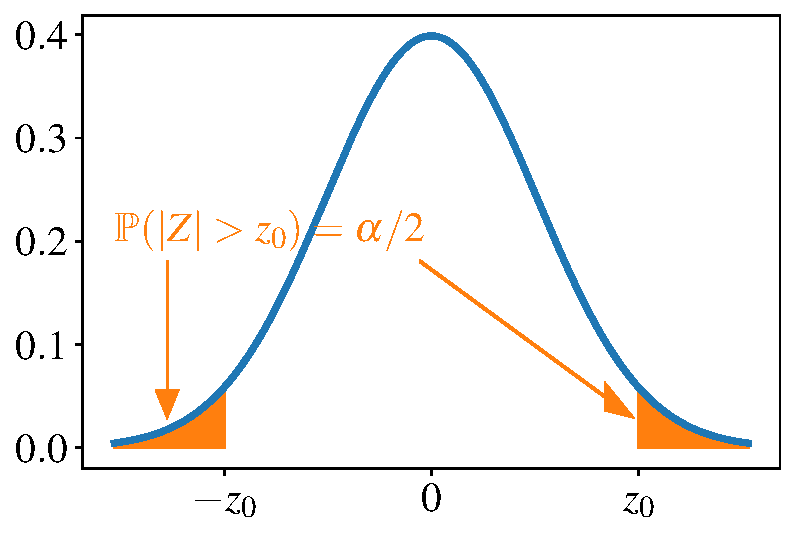
\includegraphics[width=0.5\textwidth]{figures/tests/z_moyenne}
	\caption{Densité d'une gaussienne centrée réduite. L'aire colorée vaut
		$\alpha$ et correspond au domaine de rejet du test.}
	\label{fig:z_moyenne}
\end{figure}

\paragraph{Question :} Peut-on rejeter l'hypothèse selon laquelle les pigeons
du jardin du Luxembourg ont un poids moyen de 300g ?
\bigskip

\begin{answer}
	Cela dépend du niveau de signification que l'on choisit.
	
	Calculons tout d'abord la réalisation de la statistique de test $Z$ sur notre
	échantillon : $z = 2,45.$
	
	Posons $\alpha = 0,05.$ Alors $z_0 \approx 1,96.$ On a bien $z > z_0$ et on
	rejette l'hypothèse nulle. On dit que l'écart entre $M_n$ et $\mu_0$ est
	\textbf{statistiquement significatif.}
	
	Posons maintenant $\alpha = 0,01.$ Le domaine de rejet est plus restreint ;
	$z_0 \approx 2,58.$ On ne peut pas rejeter l'hypothèse nulle. L'écart entre
	$M_n$ et $\mu_0$ n'est pas statistiquement significatif.
	
	
	Cet exemple est illustré sur la figure~\ref{fig:z_pigeons}.
\end{answer}


\begin{figure}[h]
	\centering
	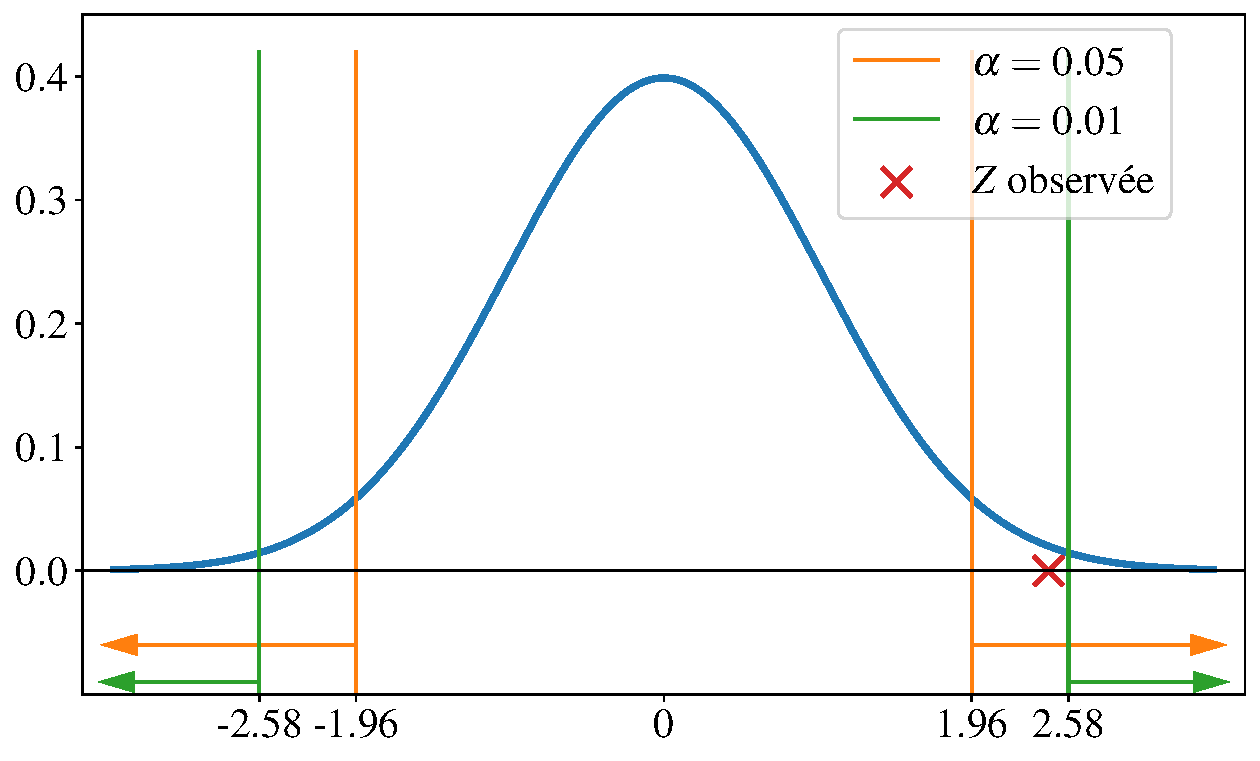
\includegraphics[width=0.65\textwidth]{figures/tests/z_pigeons}
	\caption{Densité d'une gaussienne centrée réduite. La valeur $z=2,45$ est
		dans le domaine de rejet pour $\alpha = 0,05$ mais pas pour
		$\alpha = 0,01$.}
	\label{fig:z_pigeons}
\end{figure}

\subsection{p-valeur}
\paragraph{Question :} Quelle est la p-valeur correspondant à la valeur de test
$z=2,45$ ?
\bigskip

\begin{answer}
	La p-valeur est
	\[
	\PP(\abs{Z} \geq \abs{z}) = \PP(Z \leq -\abs{z}) + \PP(Z \geq \abs{z}) = 2
	\PP(Z \leq -\abs{z}) = 2 \Phi(-\abs{z}) = 0,018.
	\]
	où $\Phi$ est la fonction de répartition d'une gaussienne standard.
	
	Cette p-valeur est bien inférieure au seuil de signification $\alpha = 0,05$,
	mais supérieure au seuil de signification $\alpha = 0,01$.
\end{answer}

\subsection{Test unilatéral à droite}
Supposons maintenant que nous nous demandons si les pigeons du Jardin du
Luxembourg, qui nous semblent particulièrement bien nourris de restes des
sandwicheries environnantes, ne seraient pas plus lourds que la moyenne de
300g. Il s'agit maintenant de faire un test unilatéral à droite, pour lequel
\[
\HH_1 : \mu > \mu_0.
\]

\paragraph{Question :} Comment cela transforme-t-il notre test d'hypothèse ?
\bigskip

\begin{answer}
	Le test statistique consiste maintenant à rejeter $\HH_0$ si $Z > z_r$ (sans
	valeur absolue). En particulier, toutes les valeurs négatives nous font
	accepter $\HH_0$, contrairement au cas bilatéral.
	
	La valeur critique $z_r$ est telle que 
	\[
	\PP(Z > z_r) = \alpha, \text{ sachant } Z \sim \Ncal(0, 1).
	\]
	La densité de $Z$ étant symmétrique, on cherche donc $z_0$ telle que 
	\[
	\Phi(-z_r) = \alpha.
	\]
	
	Pour $\alpha = 0,05,$ la valeur critique est $z_r = 1,64.$ Pour
	$\alpha = 0,01,$ la valeur critique est $z_r = 2,33.$ L'hypothèse nulle est
	rejetée dans les deux cas.
	
	Le test unilatéral est plus puissant pour les valeurs du bon côté.
	
	Cet exemple est illustré sur la figure~\ref{fig:z_pigeons_unilateral}.
\end{answer}


\begin{figure}[h]
	\centering
	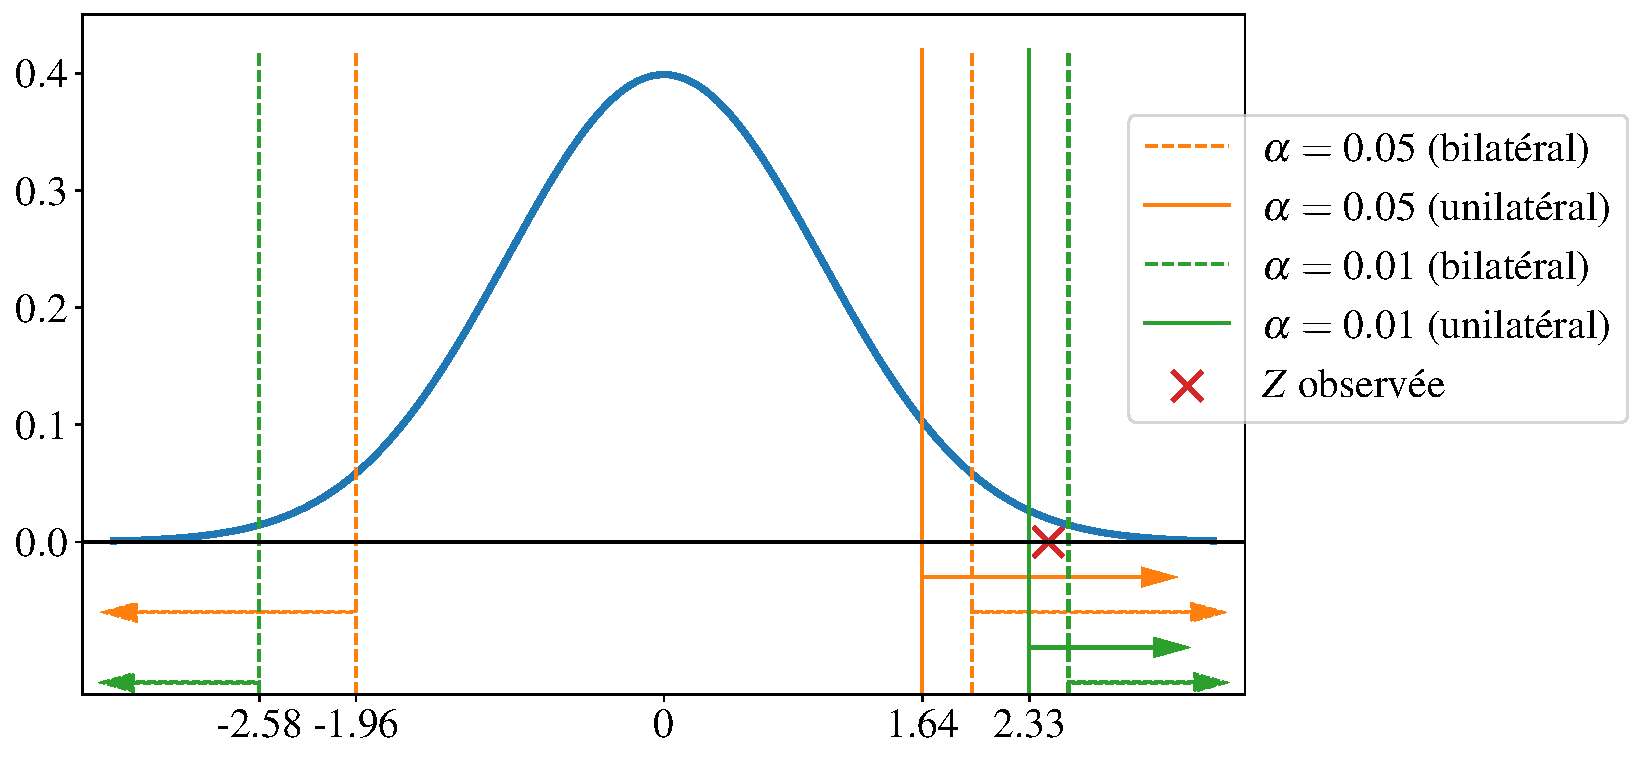
\includegraphics[width=0.85\textwidth]{figures/tests/z_pigeons_unilateral}
	\caption{Densité d'une gaussienne centrée réduite. La valeur $z=2,45$ est
		dans le domaine de rejet pour $\alpha = 0,05$ et pour $\alpha = 0,01$ dans
		le cas du test unilatéral.}
	\label{fig:z_pigeons_unilateral}
\end{figure}

\subsection{Intervalle de confiance $\bullet$}
\label{sec:ic}
Reprenons le test bilatéral.

Étant donné $\alpha,$ nous avons déterminé $z_0$ de sorte à ce que
\[
\PP(\abs{Z} > z_0) = \alpha, \text{ sachant } Z \sim \Ncal(0, 1).
\]

En d'autres termes, 
\[
\PP(-z_0 \leq Z \leq z_0) = 1 - \alpha. 
\]
(On pourra se référer à la figure~\ref{fig:z_moyenne}.)

D'après la définition de $Z$ (équation~\eqref{eq:z_moyennes}), cela est équivalent à 
\[
\PP\left( M_n - \frac{\hatsigma}{\sqrt{n}} z_0 \leq 
\mu \leq M_n + \frac{\hatsigma}{\sqrt{n}}z_0 \right) = 1 - \alpha.
\]

Ainsi l'intervalle 
\[
\left[ M_n - \frac{\hatsigma}{\sqrt{n}} z_0, \; M_n +
\frac{\hatsigma}{\sqrt{n}} z_0 \right]
\]
est un \textbf{intervalle de confiance} à $(1 - \alpha)$ pour la taille moyenne
$\mu$ (voir Probabilités V).

Dans notre exemple, l'intervalle de confiance à 95\% pour la valeur moyenne du
poids d'un pigeon est $[302,4\si{g}~; 321,6\si{g}]$.
$\mu_0 = 300\si{g}$ n'est pas dans l'intervalle de confiance ; on adopte l'hypothèse
alternative selon laquelle $\mu \neq \mu_0.$

L'intervalle de confiance à 99\% est $[299,4\si{g}~; 324,6\si{g}].$ Cet
intervalle contient $\mu_0$. On ne peut pas rejeter l'hypothèse nulle.

\paragraph{Exercice :} Calculer l'intervalle de confiance à 95\% et à 99\% pour
le test d'hypothèse unilatéral à droite. (Solution : cf section~\ref{sec:ic_sol}.)
% \section{Test d'indépendance du $\chi^2$}
% \label{sec:chi2}

\subsection{Tests de comparaison de moyenne $\bullet \bullet$} 
Le test que nous avons étudié dans cette section, qui permet de comparer la
moyenne d'un échantillon suffisamment large pour être dans la limite du
théorème centrale limite ($n \geq 30$) à sa moyenne théorique, s'appelle un
\textbf{test Z}, ou \textit{Z-test} en anglais, par référence à la notation $Z$
couramment utilisée pour une variable normalement distribuée de moyenne 0 et
variance 1.

Dans le cas d'un échantillon de faible taille, le théorème central limite ne
s'applique pas. Si l'on suppose $X$ normalement distribuée, on peut alors
appliquer un test de Student, ou test t (\textit{t-test} en anglais), ainsi
appelé car la statistique de test suit une loi de Student.

Des variantes de ces tests Z et t peuvent aussi être utilisés pour comparer les
moyennes de deux échantillons, appariés ou non. Deux échantillons aléatoires
$(X_1, X_2, \dots, X_n)$ et $(Y_1, Y_2, \dots, Y_n)$ sont dit appariés quand
les variables $X_i$ et $Y_i$ décrivent le même individu $i$. Il peut par
exemple s'agir de mesures répétées sur les mêmes individus, soit prises par
deux appareils différents, soit prises avant et après un traitement.



\section{Tests d'hypothèses multiples}
\label{sec:mht}
\paragraph{Question} Imaginons l'expérience de pile ou face suivante : je lance
15 fois une pièce équilibrée, et demande à Alice, qui est assise en face de
moi, de prédire avant chaque lancer si je vais obtenir pile ou face. Supposons
qu'Alice me donne la bonne réponse 12 fois. A-t-elle un don de
voyance ?
\bigskip

\begin{answer}
	Pour répondre à cette question, posons $X$ une variable de Bernouilli de
	paramètre $p$ modélisant, pour un lancer de pièce, le succès d'Alice :
	$X$ vaut 0 si Alice n'a pas donné la bonne prédiction et 1
	sinon. L'hypothèse nulle est
	\[
	\HH_o : p = 0,5 \text{ (Alice n'a pas de don de voyance)}.
	\]
	Nous pouvons ici poser une hypothèse alternative unilatérale à droite :
	\[
	\HH_1 : p > 0,5 \text{ (Alice a un don de voyance)}.
	\]
	Il s'agit du test binomial que nous avons défini dans la
	section~\ref{sec:formalisme_test}, mais ici la variable modélise non pas le
	résultat du lancer de pièce mais le statut (correct ou non) de la réponse
	donnée par Alice.
	
	La statistique de test $T$ est le nombre de succès dans l'échantillon. Sous
	$\HH_0$, $T \sim \Bcal(n, p).$ La p-valeur correspondant à 12 succès est donc
	$\PP_{\HH_0}(T \geq 12) = 1 - \PP(T \leq 11) = 0,018$. Cette p-valeur est
	significative pour $\alpha = 5\%$.
\end{answer}

\paragraph{Question} Supposons maintenant que je fasse ce test avec toute la
classe (sans communication entre les élèves). Trois élèves passent mon test de
psychisme, autrement dit tombent juste au moins 12 fois sur 15. Dois-je appeler
la presse ?
\bigskip

\begin{answer}
	Supposons une promo de $m=127$ élèves. Nous posons maintenant $Y$ une
	variable de Bernouilli de paramètre $\pi$ modélisant le succès d'une personne
	sur 15 lancers. Nous faisons ici un nouveau test statistique sur $Y$,
	\[
	\HH_0^\prime : \pi = 0,018 \text { \qquad et \qquad} \HH_1^\prime : \pi >
	0,018.
	\]
	Il s'agit toujours d'un test binomial. La statistique de test $U$ est le
	nombre d'élèves passant le test. Sous $\HH_0^\prime$, $U \sim \Bcal(m,
	\pi)$.
	La p-valeur est ici
	$\PP_{\HH_0^\prime}(T \geq 3) = 1 - \PP(T \leq 2) = 0,40.$ Cette p-valeur
	n'est pas significative !
\end{answer}

Cet exemple illustre le principe suivant : plus on fait de tests, et plus on a
de chances de voir apparaître une p-valeur significative. 

Il est nécessaire de corriger cet effet : on parle de \textbf{correction} ou
\textbf{ajustement de tests d'hypothèse multiples.} La plus simple et plus
utilisées de ces corrections, proposée par la biostatisticienne Olive Jean
Dunn, est connue sous le nom de \textbf{correction de Bonferroni} : il s'agit
simplement de diviser le niveau de signification par le nombre de tests
\[
\alpha \leftarrow \frac{\alpha}{m}.
\]

Cette correction se justifie de la façon suivante : notons
$p_1, p_2, \dots, p_m$ les p-valeurs obtenue pour $m$ tests, testant chacun
$\HH_0$ vs. $\HH_1$, et supposons que $\HH_0$ est vraie pour les $m_0$ premiers
tests. Alors la probabilité de rejeter au moins une de ces hypothèses nulles est
\[
\PP\left(\bigcup_{i=1}^{m_0} \left( p_i \leq \frac{\alpha}{m} \right)\right)  \leq
\sum_{i=1}^{m_0} \PP \left( p_i \leq \frac{\alpha}{m} \right)= \frac{m_0
	\alpha}{m} \leq \alpha.
\]



% \section{Compléments}
\section{Solution de l'exercice section~\ref{sec:ic} $\bullet$}
\label{sec:ic_sol}
Nous avons déterminé la valeur critique $z_r$ de sorte à ce que 
\[
\PP(Z \leq z_r) = 1-\alpha.
\]

Comme $Z = \frac{\sqrt{n} (M_n - \mu_0)}{\hatsigma}$, cela est équivalent à 
\[
\PP \left(\mu \geq M_n - \frac{\hatsigma}{\sqrt{n}} z_r \right) = 1 - \alpha.
\]

Ainsi l'intervalle 
\[
\left[M_n - \frac{\hatsigma}{\sqrt{n}} z_r, +\infty \right]
\]
est un intervalle de confiance unilatéral à $(1-\alpha)$ pour la taille moyenne $\mu$.

Dans notre exemple, l'intervalle de confiance unilatéral à droite à 95\% pour
la valeur moyenne du poids d'un pigeon est $[303,9\si{g}, +\infty]$. Cet
intervalle contient $\mu_0$ et on ne peut pas rejeter l'hypothèse nulle.  À
99\%, cet intervalle est $[300,6\si{g}, +\infty[.$ Ces résultats sont
cohérents.

\begin{plusloin}
\item On dit d'un test statistique qu'il est sans biais si sa puissance est
  supérieure au niveau de signification : $1 - \beta > \alpha$.
\item On dit d'un test statistique qu'il converge si la suite des erreurs de
  deuxième espèce converge vers $0$ : $1 - \beta \cvn 0.$ 
\item Pour plus de détails sur la sur-interprétation des p-valeurs en sciences
  et le \textit{p-hacking} (consistant à ne conserver, parmi de nombreux tests
  conduits sur les données, ceux qui donnent des p-valeurs significatives), on
  pourra se reporter aux références suivantes.
  \begin{thebibliography}{99}
  \bibitem{ioannidis2005}
    John PA Ioannidis.
    {Why most published research findings are false.}
    \textit{PLoS medicine,} 
    2(8):{e124},
    {2005.}

  \bibitem{head2015}
    Megan L Head, Luke Holman, Rob Lanfear, Andrew T Kahn and Michael D Jennions.
    {The extent and consequences of p-hacking in science.}
    \textit{PLoS biology},
    13(3):{e1002106},
    {2015.}
  \bibitem{wasserstein2016}
    Ronald L Wasserstein, Nicole A Lazar, et al.
    {The ASA's statement on p-values: context, process, and purpose}.
    \textit{The American Statistician},
    70(2):129--133,
    2016.

  \bibitem{holmes2018}
    Susan Holmes.
    {Statistical proof? The problem of irreproducibility}.
    \textit{Bulletin (New Series) of the American Mathematical Society},
    {55}(1), 2018.
  \end{thebibliography}
\end{plusloin}

%-*- coding: utf-8 -*-
\section{QCM}

\paragraph{Question 1.} Dans une étude dont le but est de déterminer si la
consommation de chocolat noir améliore les résultats scolaires, l'hypothèse
alternative est :
\begin{itemize}
\item[$\square$] Les élèves qui consomment du chocolat noir obtiennent les
  mêmes résultats que les élèves qui n'en consomment pas.
\item[$\square$] Les élèves qui consomment du chocolat noir obtiennent de moins
  bons résultats que les élèves qui n'en consomment pas.
\item[$\square$] Les élèves qui consomment du chocolat noir obtiennent de
  meilleurs résultats que les élèves qui n'en consomment pas.
\item[$\square$] Les élèves qui consomment du chocolat noir obtiennent des
  résultats différents des élèves qui n'en consomment pas.
\end{itemize}

\paragraph{Question 2.} La p-valeur est :
\begin{itemize}
\item[$\square$] La probabilité que l'hypothèse nulle soit vraie.
\item[$\square$] La probabilité que l'hypothèse alternative soit vraie.
\item[$\square$] La probabilité, si l'hypothèse nulle est vraie, d'obtenir une
  situation au moins aussi surprenante que celle observée.
\item[$\square$] La probabilité, si l'hypothèse alternative est vraie,
  d'obtenir une situation au moins aussi surprenante que celle observée.
\end{itemize}

\section*{Solution}
{%
\noindent
\rotatebox[origin=c]{180}{%
\noindent
\begin{minipage}[t]{\linewidth}
\paragraph{Question 1.}
L'hypothèse alternative est que les élèves qui consomment du chocolat noir
obtiennent de meilleurs résultats que les élèves qui n'en consomment pas. Il
s'agit d'un test unilatéral. Le test sera plus puissant que si on utilise
l'hypothèse alternative bilatérale (les résultats entre les deux groupes sont
différents). Cependant, si ce test unilatéral ne permet pas de rejeter
l'hypothèse nulle, il sera impossible de déterminer si c'est parce qu'il n'y a
pas de différence entre les deux groupes ou parce que l'effet est dans l'autre
sens.

Remarquons enfin que corrélation n'est pas causalité : ce test permet de
déterminer si la différence de performance entre les élèves cacaophiles et les
autres est significative, mais en aucun cas si elle est \textit{due} à la
consommation de chocolat. Il est tout à fait possible que la consommation de
chocolat noir soit liée à d'autres facteurs (en particulier sociaux) qui eux
influent sur la réussite scolaire. \newline

\paragraph{Question 2.} La p-valeur est la probabilité d'obtenir une situation
au moins aussi surprenante que celle observée si l'hypothèse nulle est
vraie. Il est très important de ne pas l'interpréter comme la probabilité que
l'hypothèse nulle soit vraie : 
\[
  \PP(t \geq t_0 | \HH_0) \neq \PP(\HH_0 | t \geq t_0). 
\]
\end{minipage}%
}%

%%% Local Variables:
%%% mode: latex
%%% TeX-master: "../../sdd_2025_poly"
%%% End:


%%% Local Variables:
%%% mode: latex
%%% TeX-master: "../sdd_2025_poly"
%%% End:




\part{Analyse exploratoire}
\vspace{1cm}
\chapter{Réduction de dimension}
%-*- coding: utf-8 -*-
\label{chap:dimred}

\paragraph{Notions :} sélection de variables ; extraction de variables ;
 analyse en composantes principales ; analyse en composantes principales probabiliste.
\paragraph{Objectifs pédagogiques :} 
\begin{itemize}      
  \setlength{\itemsep}{3pt}
\item Expliquer l'intérêt de réduire la dimension d'un jeu de données ;
\item Faire la différence entre la sélection de variables et l'extraction de variables ;
% \item Mettre en \oe{}uvre des méthodes de sélection de variable par filtrage ;
\item Projeter des données sur un espace de plus petite dimension ;%par factorisation de matrice ; 
\item Mettre en \oe{}uvre des méthodes d'extraction de variables.
\end{itemize}

\section{Des séries statistiques aux jeux de données}
Nous avons jusqu'à présent travaillé sur des séries statistiques contenant une
seule variable. Cependant, dans la majorité des problèmes de sciences des
données, nous disposons de plusieurs variables pour décrire chaque individu.

L'objet de nos études, à savoir le jeu de données, n'est donc plus un
échantillon $(x_1, x_2, \dots, x_n)$ d'une variable aléatoire rélle $X$, mais
un échantillon d'un vecteur aléatoire à valeurs dans un espace $\XX$. Nous
considèrerons en général que $\XX = \RR^p$ et que notre jeu de données peut
être décrit par une matrice $X \in \RRnp$.  C'est par exemple la
matrice de taille $31 \times 8$ des entrées du tableau~\ref{tab:meteo_data}.

Cela suppose que nous disposions d'une représentation $p$-dimensionnelle
pertinente de nos données. Si celle-ci est assez évidente pour des données
comme celles du tableau~\ref{tab:meteo_data}, ce n'est pas toujours le cas. En
particulier, les variables qualitatives (comme la colonne « âge » du
tableau~\ref{tab:remboursement_data}) doivent être représentées par un (ou
plusieurs) nombres réels. 

Nous supposons dans ce cours que nos données sont présentées sous forme
vectorielle ; on parle parfois de données \textbf{structurées}. Ce n'est pas le
cas de nombreux types de données telles que du texte, des images, du son, des
séquences d'ADN, ou des molécules chimiques. La question de la représentation
de ces données dites non-structurées dépasse le cadre de ce cours mais est très
importante.

\section{Notations}
Nous essaierons à partir de maintenant de nous en tenir aux notations suivantes
:
\begin{itemize}
\item Les lettres minuscules ($x$) représentent un scalaire ;
\item les lettres minuscules surmontées d'une flèche ($\xx$) représentent un
  vecteur ;
\item les lettres majuscules ($X$) représentent une matrice, un événement ou
  une variable aléatoire ;
\item les lettres calligraphiées ($\XX$) représentent un ensemble ou un espace ;
\item les {\it indices} correspondent à une variable tandis que les {\it
    exposants} correspondent à une observation : $x^i_j$ est la $j$-ème
  variable de la $i$-ème observation, et correspond à l'entrée $X_{ij}$ de la
  matrice $X$ ;
\item $n$ est un nombre d'observations et $p$ un nombre de variables.
\end{itemize}

\section{Motivation $\bullet$}
Le but de la réduction de dimension est de transformer une représentation
$X \in \RRnp$ des données en une représentation
$X^* \in \RR^{n \times m}$ où $m \ll p$. Les raisons de cette démarche sont
multiples.

\paragraph{Visualiser les données.} Ce n'est pas tâche aisée avec un nombre
très grand de variables. Comment visualiser $n$ points en plus de 2 ou 3
dimensions ? Limiter les variables à un faible nombre de dimensions permet de
visualiser les données plus facilement, quitte à perdre un peu d'information
lors de la transformation.

\paragraph{Réduire les coûts algorithmiques du traitement des données.} D'un
point de vue purement computationnel, réduire la dimension des données permet
de réduire d'une part l'espace qu'elles prennent en mémoire et d'autre part les
temps de calcul. De plus, si certaines variables sont inutiles, ou redondantes,
il n'est pas nécessaire de les obtenir pour de nouvelles observations : cela
permet de réduire le coût d'acquisition des données.

\paragraph{Améliorer la qualité du traitement des données.} Les algorithmes
d'apprentissage supervisé ou de clustering sont généralement plus performants
sur un faible nombre de variables. En effet, si certaines des variables
ne sont pas pertinentes, elles risquent de biaiser les modèles appris.\\
De plus, les raisonnements développés en faible dimension pour construire un
algorithme d'apprentissage supervisé ne s'appliquent pas nécessairement en
haute dimension. C'est un phénomène connu sous le nom de \textbf{fléau de la
  dimension}, ou \textit{curse of dimensionality} en anglais. \\
En effet, en haute dimension, les individus ont tendance à tous être éloignés
les uns des autres. Pour comprendre cette assertion, plaçons-nous en dimension
$p$ et considérons l'hypersphère $\Scal(\xx, R)$ de rayon $R \in \RR_+^*$
centrée sur une observation $\xx$, ainsi que l'hypercube $\Ccal(\xx, R)$
circonscrit à cette hypersphère. Le volume de $\Scal(\xx)$ vaut
$\frac{R^p \pi^{p/2}}{\Gamma(1+p/2)}$, tandis que celui de $\Ccal(\xx, R)$,
dont le côté a pour longueur $2R$, vaut $2^p R^p$. Ainsi
\begin{equation*}
  \lim_{p \rightarrow \infty} \frac{\text{Vol}(\Scal(\xx, R))}{
    \text{Vol}(\Ccal(\xx, R))} = 0.
\end{equation*}
Cela signifie que la probabilité qu'une observation située dans $\Ccal(\xx, R)$
appartienne à $\Scal(\xx, R)$, qui vaut $\frac{\pi}4 \approx 0.79$ lorsque
$p=2$ et $\frac{\pi}6 \approx 0.52$ lorsque $p=3$, devient très faible quand
$p$ est grand : les données ont tendance à être éloignées les unes des autres.

% Cela implique que les algorithmes développés en utilisant une notion de
% similarité ou distance entre individus ne fonctionnent pas nécessairement en
% grande dimension. Ainsi, réduire la dimension des données peut être nécessaire
% à la construction de bons modèles d'apprentissage.

Deux possibilités s'offrent à nous pour réduire la dimension de nos données :
\begin{itemize}
\item la \textbf{sélection de variables}, qui consiste à \textit{éliminer} un nombre
  $(p-m)$ de variables de nos données ;
\item l'\textbf{extraction de variables}, qui consiste à {\it créer} $m$
  nouvelles variables à partir des $p$ variables dont nous disposons
  initialement.
\end{itemize}



\section{Sélection de variables $\bullet$} 

La sélection de variables consiste à éliminer des variables peu informatives.

Dans le cas non-supervisé, il s'agit par exemple d'éliminer des variables
\begin{itemize}
\item dont la variance est très faible : leur valeur étant à peu près la même
  pour chaque individu, elles n'apportent aucune information permettant de
  distinguer deux individus ;
\item qui sont corrélées à une autre variable : elles apportent alors la même
  information et sont redondantes.
\end{itemize}

Dans le cas supervisé, il s'agit aussi d'éliminer des variables qui ne sont pas
pertinentes par rapport à la tâche de prédiction. On peut par exemple
\begin{itemize}
\item éliminer, par exemple à l'aide d'un test statistique ou une mesure de corrélation,
  les variables indépendantes de l'étiquette à prédire. Remarquez néanmoins que
  deux variables chacune indépendante de l'étiquette peuvent être très
  informatives quand on les considère simultanément. Considérez par exemple,
  pour $\XX = \zo^2$, un problème de classification binaire dans lequel
  l'étiquette $y$ est donnée par $y = x_1 \oplus x_2$ : les deux variables
  prises ensemble déterminent parfaitement $y,$ mais chacune d'entre elles
  prise individuellement est décorrélée de $y$ ;
\item chercher à éliminer des variables qui n'améliorent pas la performance
  d'un algorithme précis.
\end{itemize}
Nous reviendrons sur la
sélection de variables supervisée quand nous parlerons du lasso
(section~\ref{sec:lasso}).


%La suite de ce chapitre détaille des exemples de ces deux approches.

\section{Analyse en composantes principales $\bullet$}
\label{sec:pca}
La méthode la plus classique pour réduire la dimension d'un jeu de données par
extraction de variables est l'\textbf{analyse en composantes principales}, ou
{\it ACP}. On parle aussi souvent de {\it PCA}, de son nom anglais {\it
  Principal Component Analysis}.

\subsection{Maximisation de la variance $\bullet$}
\label{sec:variance_maximization}
L'idée est de représenter les données selon leurs axes de plus grande
variation, de sorte à pouvoir continuer à distinguer les observations les unes
des autres dans leur nouvelle représentation
(cf. figure~\ref{fig:data_variance}).  Ainsi, une ACP de la matrice
$X \in \RRnp$ est une transformation linéaire orthogonale qui permet d'exprimer
$X$ dans une nouvelle base orthonormée, de sorte à maximiser la variance de la
projection de $X$ sur les axes de cette nouvelle base. De plus, on ordonne ces
axes, appelés \textbf{composantes principales}, abrégées en {PC} pour {\it
  Principal Components}, par variance décroissante.
Plus précisément, étant donné $m \leq p$, on appelle $m$ composantes
principales de $X \in \RRnp$ une liste $(\ww_1, \ww_2, \ldots, \ww_m)$ de
vecteurs $\ww_j$ de $\RR^p$, vérifiant, pour tout $j = 1, \dots, m$ :
\begin{equation}
  \left\lbrace
    \begin{split}
      & \ww_j \in \argmax_{\ww \in \RR^p} \text{var}(X \ww) \\
      & \ltwonorm{\ww_j} = 1 \\
      & \langle \ww_j, \ww_k \rangle = 0  \text{ pour tout } k < j
    \end{split}
  \right.
  \label{eq:pc_def}
\end{equation}
  


\begin{figure}[h!]
  \centering
  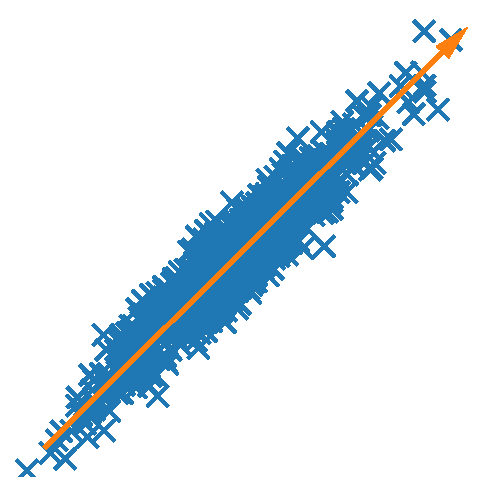
\includegraphics[width=0.3\textwidth]{figures/dimred/data_variance}
  \caption{La variance des données en deux dimensions est maximale selon l'axe
    indiqué par la flèche.}
  \label{fig:data_variance}
\end{figure}


\subsection{Standardisation}
Dans la suite de cette section, nous supposons que les variables ont été
\textbf{standardisées} de sorte à toutes avoir une moyenne de 0 et une variance
de 1, pour éviter que les variables qui prennent de grandes valeurs aient plus
d'importance que celles qui prennent de faibles valeurs. C'est un pré-requis de
l'application de l'ACP.  Cette standardisation s'effectue par :
\begin{equation}
  \label{eq:standardization}
  x^i_j \leftarrow \frac{x^i_j - \overline{x_j}}{\sqrt{\frac1n 
      \sum_{l=1}^n (x^l_j - \overline{x_j})^2}},
\end{equation}
où $\overline{x_j} = \frac1n \sum_{l=1}^n x^l_j.$ On dira alors que $X$ est
\textbf{centrée} : chacune de ses colonnes a pour moyenne 0 et \textbf{réduite} :
chacune de ses colonnes a pour variance 1.

\begin{exemple}
  Considérons la matrice de données 
  \[
    X = \begin{bmatrix} 1.0 & 20.0 \\
      2.0 & 10.0 \\
      3.0 & 50.0 \\
      4.0 & 30.0 \\
      5.0 & 40.0 \\
    \end{bmatrix}.
  \]
  La variance de la première colonne vaut $2.0$ tandis que celle de la deuxième
  colonne vaut $200.0$. Peut-on pour autant en conclure que la deuxième
  variable « varie » plus que la première, alors que les valeurs qu'elle prend
  sont simplement proportionnelles à celles prises par la première ?

  La version standardisée de $X$ est
  \[
    \begin{bmatrix} -1.414 & -0.707 \\
      -0.707 & -1.414 \\
      0.0 & 1.414 \\
      0.707 & 0.0 \\
      1.414 & 0.707 
    \end{bmatrix}.
  \]
\end{exemple}


\subsection{Décomposition spectrale de la covariance $\bullet$}
\paragraph{Matrice de covariance} La matrice de covariance empirique d'une matrice de
données $X \in \RRnp$ est une matrice $\Sigma \in \RRpp$ telle que
$\Sigma_{jk} = \text{cov}\left(\xx_j, \xx_k \right)$ pour tout
$j, k = 1, \ldots, p$. Ici $\xx_j \in \RR^n$ représente la série statistique
composée des $n$ observations de la $j$-ème variable. Ainsi, si les données
sont centrées-réduites,
\[
  \Sigma_{jk} = \frac1n \sum_{i=1}^n (x_j^i - \overline{x_j})  (x_k^i - \overline{x_k}) = \frac1n \sum_{i=1}^n x_j^i x_k^i
   = \frac1n \langle \xx_j, \xx_k \rangle
 \]
 et $\Sigma = \frac1n X^\top X$ est une matrice symétrique avec $\frac1n$ sur la diagonale (car $\Sigma_{jj} = \text{var}(\xx_j) = 1$).

\paragraph{Proposition} 
Soit $X \in \RRnp$ une matrice centrée et 
$\Sigma = \frac1n X^\top X$ sa matrice de covariance empirique. Les composantes principales de $X$ sont les
vecteurs propres de $\Sigma$, ordonnés par valeurs propres décroissantes.

\paragraph{Preuve  $\bullet\bullet$}
\begin{itemize}
\item Considérons un vecteur $\ww \in \RR^p$. 
La moyenne de $X \ww$ vaut $0$ car les variables $(\xx_1, \dots, \xx_p)$ sont
elles-mêmes de moyenne nulle ($X$ étant centrée).
La variance de $X \ww$ vaut donc 
\begin{equation*}
  \text{var}(X \ww) = \frac1n \sum_{i=1}^n \left( \sum_{j=1}^p x_j^i w_j \right)^2 = \ww^\top \Sigma \ww.
\end{equation*}    
\item Appelons maintenant $\ww_1 \in \RR^p$ la première composante principale de $X$.
$\ww_1$ est de norme $1$ et telle que la variance de $X \ww_1$ est maximale :
\begin{equation}
  \label{eq:pc1}
  \ww_1 \in \argmax_{\ww \in \RR^p} \left( \ww^\top \Sigma \ww \right)  \text{\qquad avec } \ltwonorm{\ww_1}^2=1.
\end{equation}
Il s'agit d'un problème d'optimisation quadratique sous contrainte d'égalité,
que l'on peut résoudre (cf section 2.2.1 du poly d'Optimisation) en
introduisant le multiplicateur de Lagrange $\alpha_1 > 0$ et en écrivant le
lagrangien
\begin{equation*}
  L(\alpha_1, \ww) = \ww^\top \Sigma \ww - \alpha_1 
  \left( \ltwonorm{\ww}^2 - 1 \right).
\end{equation*}
%Par dualité forte, % $\min_{\ww \in \RR^p} w^\top \Sigma w = \max_{\alpha_1}
    % \inf_{\ww \in \RR^p} L(\alpha_1, \ww).$
Le maximum de $\ww^\top \Sigma \ww$ sous la contrainte $\ltwonorm{\ww_1}^2=1$ est
égal à $\min_{\alpha_1} \sup_{\ww \in \RR^p} L(\alpha_1, \ww).$ Le supremum du
lagrangien est atteint en un point où son gradient s'annule, c'est-à-dire qui
vérifie
\begin{equation*}
  2 \Sigma \ww - 2 \alpha_1 \ww = 0.
\end{equation*}
Ainsi, $\Sigma \ww_1 = \alpha_1 \ww_1$ et $(\alpha_1, \ww_1)$ forment un couple
(valeur propre, vecteur propre) de $\Sigma$.

Parmi tous les vecteurs propres de $\Sigma$, $\ww_1$ est celui qui maximise la
variance $\ww_1^\top \Sigma \ww_1 = \alpha_1 \ltwonorm{\ww_1} = \alpha_1.$
Ainsi, $\alpha_1$ est la plus grande valeur propre de $\Sigma$ (rappelons que
$\Sigma$ étant définie par $X^\top X$ est semi-définie positive et que toutes
ses valeurs propres sont positives).

\item La deuxième composante principale de $X$ vérifie
\begin{equation}
  \label{eq:pc2}
  \ww_2 = \argmax_{\ww \in \RR^p} \left( \ww^\top \Sigma \ww \right) \text{ \qquad avec } \ltwonorm{\ww_2}^2=1
  \text{ et } \ww_2^\top\ww_1=0.
\end{equation}

Nous introduisons donc maintenant deux multiplicateurs de Lagrange
$\alpha_2 > 0$ et $\beta_2 > 0$ et obtenons le lagrangien
\begin{equation*}
  L(\alpha_2, \beta_2, \ww) = \ww^\top \Sigma \ww - \alpha_2 
  \left(\ltwonorm{\ww}^2 - 1 \right)
  - \beta_2 \ww^\top\ww_1.
\end{equation*}
Comme précédemment, son supremum en $\ww$ est atteint en un point où son
gradient s'annule :
\begin{equation*}
  2 \Sigma \ww_2 - 2 \alpha_2 \ww_2 - \beta_2 \ww_1 = 0.
\end{equation*}
En multipliant à gauche par $\ww_1^\top$, on obtient
\begin{equation*}
  2 \ww_1^\top \Sigma \ww_2 - 2 \alpha_2 \ww_1^\top \ww_2 - 
  \beta_2 \ww_1^\top \ww_1 = 0.
\end{equation*}
Comme $\ww_1^\top \Sigma \ww_2 = 0$ puisque les $\xx_j$ sont centrées, et que
$\ww_1^\top \ww_2 = 0$ et $\ww_1^\top \ww_1 = 1$ par définition
(équation~\eqref{eq:pc2}), on en conclut que $\beta_2=0.$ En remplaçant dans
l'équation précédente, comme pour $\ww_1$, on obtient
$2 \Sigma \ww_2 - 2 \alpha_1 \ww_2 = 0$.  Ainsi $(\alpha_2, \ww_2)$ forment un
couple (valeur propre, vecteur propre) de $\Sigma,$ distinct de
$(\alpha_1, \ww_1),$ et $\alpha_2$ est maximale : il s'agit donc nécessairement
de la deuxième valeur propre de $\Sigma$.
    
\item Le raisonnement se poursuit de la même manière pour les composantes principales
  suivantes.
\end{itemize}
\hfill $\square$

  
\paragraph{Preuve alternative  $\bullet\bullet$} Alternativement, on peut prouver ce théorème
en observant que $\Sigma$, étant définie positive, est
diagonalisable par un changement de base orthonormée :
$\Sigma = Q^\top \Lambda Q$, où $\Lambda \in \RRpp$ est une
matrice diagonale dont les valeurs diagonales sont les valeurs propres de
$\Sigma$.  Ainsi,
\begin{equation*}
  \ww_1^\top \Sigma \ww_1 = \ww_1^\top Q^\top \Lambda Q \ww_1 = 
  \left(Q \ww_1 \right)^\top \Lambda \left(Q \ww_1 \right).
\end{equation*}
Si l'on pose $\vv = Q \ww_1$, il s'agit donc pour maximiser
$\ww_1^\top \Sigma \ww_1$ de trouver $\vv$ de norme 1 ($Q$ étant orthonormée et
$\ww_1$ de norme 1) qui maximise
\[\sum_{j=1}^p v_j^2 \lambda_j.\]  

Pour tout $j=1, \dots, p$, on a $\lambda_j \geq 0$ (car $\Sigma$ est définie
positive) et $0 \leq v_j^2 \leq 1$ car $\ltwonorm{\vv} = 1$. Ainsi, 
\[\sum_{j=1}^p v_j^2 \lambda_j \leq 
\left(\max_{j=1, \dots, p} \lambda_j \right)\sum_{j=1}^p
v_j^2 \leq \max_{j=1, \dots, p} \lambda_j,\]
et ce maximum est atteint quand $v_j=1$ et $v_k=0 \text{ pour tout } k \neq j$. On
retrouve ainsi que $\ww_1$ est le vecteur propre correspondant à la plus grande
valeur propre de $\Sigma$, et ainsi de suite. \hfill $\square$


\subsection{Décomposition en valeurs singulières $\bullet\bullet$}
\paragraph{Définition/Proposition} Toute matrice $X \in \RRnp$ peut être
décomposée sous la forme $X = U D V^\top,$ avec $U \in \RR^{n \times n}$ et
$V \in \RRpp$ orthogonales et $D \in \RRnp$ une matrice diagonale positive
(c'est-à-dire que ses coefficients diagonaux $D_{ii}$ pour
$i=1, \dots, \min(n, p)$ sont positifs ou nuls et les coefficients hors
diagonale sont nuls).

Cette décomposition est appelée \textbf{décomposition en valeurs singulières},
ou \textit{SVD} pour \textit{Singular Value Decomposition}, et les
coefficients diagonaux $D_{ii}$ sont les \textbf{valeurs singulières} de $X$,
c'est-à-dire les racines des valeurs propres de $X^\top X$. 

\paragraph{Preuve} La matrice $X^\top X$ étant positive semi-définie, il existe d'après le théorème spectral une matrice orthogonale $V \in \RRpp$ telle que
\begin{equation}
  V^\top \left( X^\top X\right) V =
  \begin{bmatrix}
    \Delta & 0 \\
    0 & 0
  \end{bmatrix}
  \label{eq:diag_xtx}
\end{equation}
avec $\Delta \in \RR^{r \times r}$ diagonale, de coefficients strictement positifs, de même rang $r \leq \min(n, p)$ que $X.$ 

En décomposant $V$ en deux blocs : $V =
\begin{bmatrix}
  V_1 & V_2 \\
\end{bmatrix}$ avec $V_1 \in \RR^{p \times r}$ et $V_2 \in \RR^{p \times (p-r)}$, on peut réécrire l'équation~\eqref{eq:diag_xtx} comme
\begin{equation*}
  \begin{bmatrix}
    V_1^\top X^\top X V_1 & V_1^\top X^\top X V_2 \\
    V_2^\top X^\top X V_1 & V_2^\top X^\top X V_2
  \end{bmatrix} =  
  \begin{bmatrix}
    V_1^\top \\
    V_2^\top
  \end{bmatrix}  \left( X^\top X\right) 
  \begin{bmatrix}
    V_1 & V_2
  \end{bmatrix} =
  \begin{bmatrix}
    \Delta & 0 \\
    0 & 0
  \end{bmatrix}
\end{equation*}
et identifier $V_1^\top X^\top X V_1 = \Delta$.
% et $V_2^\top X^\top X V_2 = 0$, ce qui implique $X V_2 = 0$ (la trace de $V_2^\top X^\top X V_2$ étant la somme des carrés des entrées de $X V_2$).

Posons maintenant $U_1 = (X V_1) \Delta^{-1/2} \in \RR^{n \times r}.$
$U_1^\top U_1 = \Delta^{-1/2} (X V_1)^\top  (X V_1) \Delta^{-1/2} = I_r$ et on peut étendre les colonnes orthonormées de $U_1$ par $U_2 \in \RR^{n \times (n-r)}$ de sorte à former une base orthonormée de $\RRnn$ et obtenir $U =
\begin{bmatrix}
  U_1 U_2
\end{bmatrix}$ orthogonale.

Enfin, posons
\begin{equation*}
  D =
  \begin{bmatrix}
    \Delta^{1/2} & 0 \\
    0 & 0 \\
  \end{bmatrix}
\end{equation*}
avec $D \in \RR^{n \times p}$ -- autrement dit, on ajoute $(p-r) \geq 0$ colonnes de zéros
et $(n-r) \geq 0$ lignes de zéros à $\Delta^{1/2}$.

On a maintenant
\begin{equation*}
  U D V^\top =
  \begin{bmatrix}
    U_1 & U_2
  \end{bmatrix}   \begin{bmatrix}
    \Delta^{1/2} & 0 \\
    0 & 0 \\
  \end{bmatrix}
  \begin{bmatrix}
    V_1^\top \\
    V_2^\top
  \end{bmatrix} = U_1 \Delta^{1/2} V_1^\top = (X V_1) \Delta^{-1/2} \Delta^{1/2} V_1^\top = X.
\end{equation*} \hfill $\square$


\paragraph{Relation entre SVD et PCA}
Ainsi, les composantes principales d'une matrice centrée sont ses vecteurs
singuliers à droite (les colonnes de $V$), ordonnés par valeur singulière
décroissante.

\paragraph{Preuve}
Factorisons $X$ sous la forme $U D V^\top$ avec $U \in \RRnn$ et
$V \in \RRpp$ orthogonales, et $D \in \RRnp$ diagonale (c'est-à-dire que les
coefficients $D_{ij}$ pour $i \neq j$ sont nuls) dont les coefficients
diagonaux sont les valeurs singulières de $X$. Alors
\begin{equation*}
 n \Sigma = X^\top X = V D U^\top U D V^\top = V D^2 V^\top
\end{equation*}
et les valeurs singulières de $X$ (les coefficients diagonaux de $D$) sont les racines carrées
des valeurs propres de $n \Sigma$, tandis que les vecteurs singuliers à droite de
$X$ (les colonnes de $V$) sont les vecteurs propres de $n \Sigma$. \hfill $\square$
  
% En pratique, les implémentations de la décomposition en valeurs singulières (ou
% SVD) sont numériquement plus stables que celles de décomposition spectrale, et
% c'est ainsi que l'ACP est implémentée.

\subsection{Choix du nombre de composantes principales $\bullet$}
Réduire la dimension des données par une ACP implique de {\it choisir} un
nombre de composantes principales à conserver. Pour ce faire, on utilise la
\textbf{proportion de variance expliquée} par ces composantes.

La proportion de variance de la matrice de données $X \in \RRnp$ expliquée
par ses $m$ premières composantes est calculée comme :
\begin{equation}
  \label{eq:var_explained}
  \frac{\sum_{j=1}^m \text{var}(X \ww_j)}{\sum_{j=1}^p \text{var}(X \ww_j)} = \frac{\alpha_1 + \alpha_2 + \dots + \alpha_m}{\text{trace}(\Sigma)},
\end{equation}
où $\alpha_1 \geq \alpha_2 \geq \dots \geq \alpha_p$ sont les valeurs propres
de $\Sigma$ par ordre décroissant.
  
Il est classique de s'intéresser à l'évolution, avec le nombre de composantes,
soit de la proportion de variance expliquée par chacune d'entre elles, soit à
cette proportion cumulée. On peut représenter visuellement ces proportions sur
un {\it scree plot} (figure~\ref{fig:scree_plots}), utilisé pour déterminer le
nombre de composantes qui expliquent ensemble un pourcentage de la variance
fixé a priori ($95\%$ sur la figure~\ref{fig:scree_plot_cumul}), ou le nombre
de composantes à partir duquel ajouter une nouvelle composante n'est plus
informatif («~coude~» sur la
figure~\ref{fig:scree_plot}). % Ce graphe peut nous servir
% à déterminer visuellement soit le nombre de composantes principales qui
% expliquent un pourcentage de la variance que l'on s'est initialement fixé
% ($95\%$ sur la figure~\ref{fig:scree_plot}, soit le nombre de composantes
% principales correspondant au « coude » du scree plot cumulatif
% (figure~\ref{fig:scree_plot_cumul}), à partir duquel ajouter une nouvelle
% composante ne semble plus informatif.


\begin{figure}[h]
  \begin{subfigure}[t]{0.43\textwidth}
    \centering
    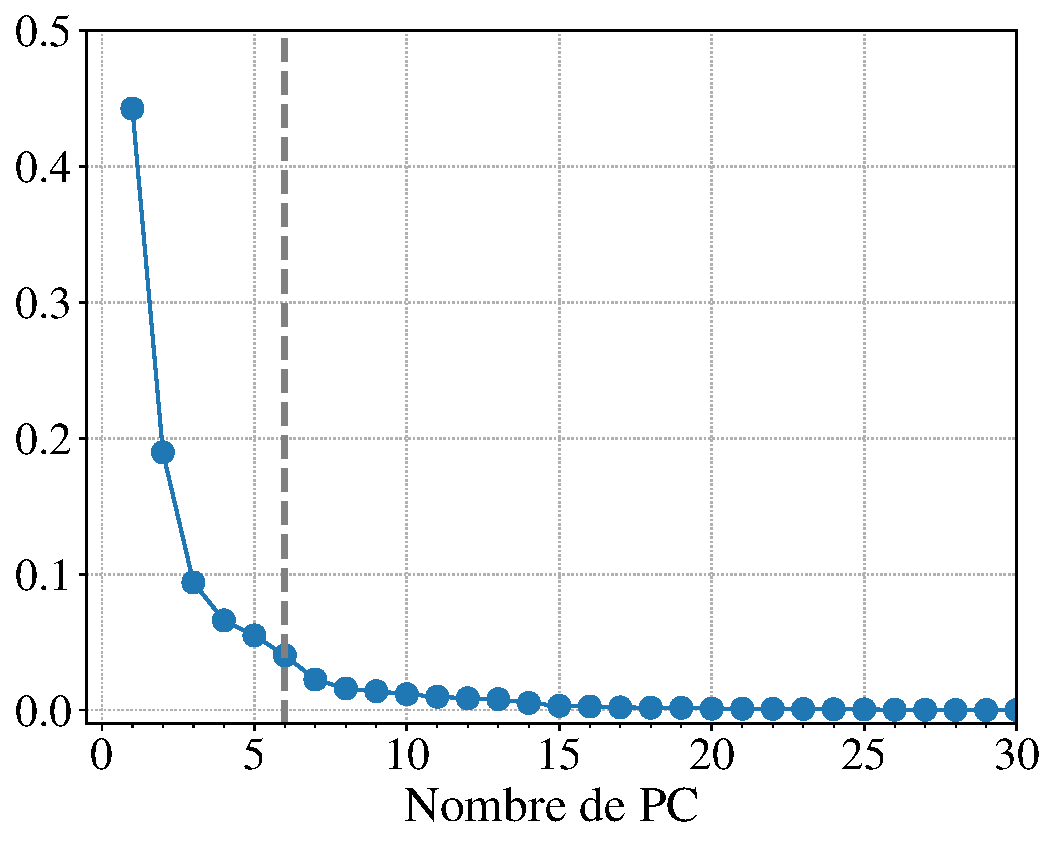
\includegraphics[width=\textwidth]{figures/dimred/scree_plot}
    \caption{Proportion de variance expliquée par chacune des composantes
      principales. À partir de 6 composantes principales, ajouter de nouvelles
      composantes n'est plus vraiment informatif.}
    \label{fig:scree_plot}
  \end{subfigure} \hfill
  \begin{subfigure}[t]{0.43\textwidth}
    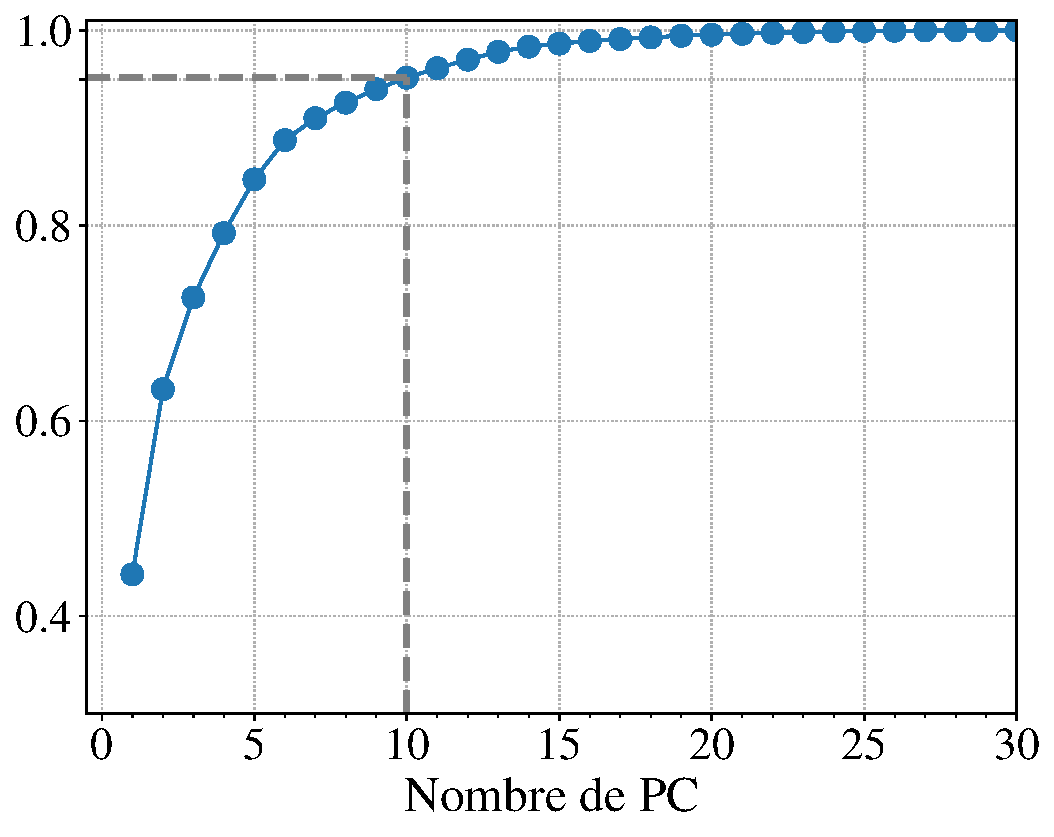
\includegraphics[width=\textwidth]{figures/dimred/scree_plot_cumul}  
    \caption{Proportion cumulée de variance expliquée par chacune des
      composantes principales. Si on se fixe une proportion de variance
      expliquée de $95\%$, on peut se contenter de 10 composantes principales.}
    \label{fig:scree_plot_cumul}
  \end{subfigure}
  \caption{Choix du nombre de composantes principales à l'aide de la variance expliquée.}
  \label{fig:scree_plots}
\end{figure}

\section{Factorisation de la matrice des données $\bullet$}
Soit $W \in \RRpp$ la matrice de toutes les composantes principales de
$X \in \RRnp$. Posons $m< p$ le nombre de composantes principales choisies, et
$\widetilde{W} \in \RR^{p \times m}$ la matrice des $m$ premières composantes
principales de $X$ (autrement dit la concaténation des composantes principales
$\ww_1, \ww_2, \dots, \ww_m$ exprimés comme vecteurs colonnes). La nouvelle
représentation dans $\RR^m$ d'un individu $\xx \in \RR^p$ est donnée par sa
projection sur $(\ww_1, \ww_2, \dots, \ww_m)$ :
\begin{equation}
  \label{eq:reduced_rep_vector}
  \hh = \xx \widetilde{W}.
\end{equation}

On obtient la représentation $m$-dimensionnelle des $n$ individus de $X$ par
\begin{equation}
  \label{eq:reduced_rep}
  \widetilde{H} = X \widetilde{W}.
\end{equation}

La matrice $\widetilde{H} \in \RR^{m \times n}$ peut être interprétée comme une
\textbf{représentation latente} (ou cachée, {\it hidden} en anglais d'où la
notation $H$) des données. C'est cette représentation que l'on a cherché à
découvrir grâce à l'ACP.


\subsection{Erreur de reconstruction $\bullet$}
Si on utilise toutes les composantes, la représentation latente de $X$ est donnée par 
\begin{equation}
  \label{eq:full_rep}
  H = X W; H \in \RRnp.
\end{equation}
Les colonnes de $W$ étant des vecteurs orthonormés (il s'agit de vecteurs
propres de $X^\top X$), on peut multiplier l'équation~\eqref{eq:full_rep} à
droite par $W^\top$ pour obtenir une factorisation de $X$ :
\begin{equation}
  \label{eq:pca_factor}
  X = H W^\top.
\end{equation}

En se restreignant à $m < p$ composantes, la multiplication à droite par
$\widetilde{W}^\top$ de la représentation latente $\widetilde{H}$ est une approximation de
$X$ :
\begin{equation}
  \label{eq:pca_factor_approx}
  Z = \widetilde{H} \widetilde{W}^\top.
\end{equation}
$Z \in \RRnp$ peut être interprétée comme une
\textbf{reconstruction} des données dans $\RR^p$ à partir de leur
représentation latente dans $\RR^m$.

On peut alors calculer l'\textbf{erreur de reconstruction} comme la somme des
carrés des distances entre les individus $\xx^i$ et leur reconstruction $\zz^i$ :
\begin{equation}
  \label{eq:pca_reconstruction_error}
  \text{Err}_m = \sum_{i=1}^n \norm{\xx^i - \zz^i}^2.
\end{equation}

L'erreur de reconstruction vaut 
\[
  \text{Err}_m = \sum_{i=1}^n \; \bignorm{\sum_{j=1}^p H_{ij} \ww_j - \sum_{j=1}^m H_{ij} \ww_j }^2 = 
\sum_{i=1}^n \; \bignorm{\sum_{j=m+1}^p H_{ij} \ww_j }^2 = \sum_{i=1}^n \sum_{j=m+1}^p H_{ij}^2,
\]
cette dernière égalité venant de ce que les vecteurs $\ww_j$ sont orthogonaux
et de norme 1.  Ainsi, l'erreur de reconstruction est la somme des carrés des
coefficients des dimensions qui n'ont pas été prises en compte.

Comme $H = X W$, on peut réécrire l'erreur de reconstruction comme 
\[
  \text{Err}_m = \sum_{i=1}^n \sum_{j=m+1}^p \ww_j^\top \xx^i \xx^{i\top}\ww_j
  = \sum_{j=m+1}^p \ww_j \Sigma \ww_j^\top.
\]
Ainsi, maximiser la variance $\sum_{j=1}^m \ww_j \Sigma \ww_j^\top$ est
équivalent à minimiser l'erreur de reconstruction car
$
\sum_{j=1}^p \ww_j \Sigma \ww_j^\top = \text{trace}(\Sigma).
$
C'est une autre justification de l'ACP.

\subsection{Analyse factorielle $\bullet \bullet$}
L'équation \eqref{eq:pca_factor} s'inscrit dans le cadre plus général de
\textbf{l'analyse factorielle}. Il correspond à considérer que les données sont
les réalisations d'un vecteur aléatoire $(X_1, X_2, \dots, X_p)$ obtenues par
% \begin{equation}
%   \label{eq:fa_model}
%   (X_1, X_2, \dots, X_p)^\top = (H_1, H_2, \dots, H_m)^\top W + \epsilon,
% \end{equation}
\begin{equation}
  \label{eq:fa_model}
  (X_1, X_2, \dots, X_p) = W (H_1, H_2, \dots, H_m) + \epsilon,
\end{equation}
où $(H_1, H_2, \dots, H_m)$ est le vecteur aléatoire latent qui génère les
données et $\epsilon$ un bruit gaussien : $\epsilon \sim \Ncal(0, \Psi),$ avec
$\Psi \in \RRpp$.

Supposons maintenant que $(H_1, H_2, \dots, H_m)$ est un vecteur aléatoire
gaussien $m$-dimensionnel, d'espérance $0$ (les variables latentes sont elles
aussi centrées) et de covariance $I_m$ où $I_m$ est la matrice identité de
dimensions $m \times m$. Alors $(X_1, X_2, \dots, X_p)$ est lui-même un vecteur
aléatoire gaussien, d'espérance nulle et de covariance $WW^\top + \Psi$.

Si l'on suppose de plus que $\epsilon$ est un bruit isotropique, autrement dit
que $\Psi = \sigma^2 I_p$, alors 
\[
  (X_1, X_2, \dots, X_p) \sim \Ncal (0, WW^\top + \sigma^2 I_p).
\] 
On peut alors estimer les paramètres $W$ et $\sigma^2$ par maximum de
vraisemblance ; c'est ce qu'on appelle l'\textbf{ACP probabiliste}.

L'ACP que nous venons de voir est un cas limite de l'ACP probabiliste, obtenu
quand la covariance du bruit devient infiniment petite
($\sigma^2 \rightarrow 0$)\footnote{Vous en trouverez la preuve dans l'article
  \textit{Probabilistic principal components analysis}, M.~E. Tipping \&
  C.~M. Bishop,  Journal of the Royal
    Statistical Society Series B, 61:611--622 (1999).}.

On peut plutôt faire la supposition plus générale que $\Psi$ est une matrice
diagonale. Les valeurs de $W$ et $\Psi$ peuvent une fois de plus
être obtenues par maximum de vraisemblance. C'est ce que l'on appelle
\textbf{l'analyse factorielle}.  Dans l'analyse factorielle, les composantes
principales (les colonnes de $W$) ne sont pas nécessairement orthogonales. En
particulier, il est donc possible d'obtenir des composantes dégénérées,
autrement dit des colonnes de $W$ dont toutes les coordonnées sont $0$.

\begin{plusloin}
\item Une variante populaire de l'analyse factorielle est la
  \textbf{factorisation positive de matrice} (ou NMF pour \textit{non-negative
    matrix factorisation}), qui permet lorsque toutes les entrées de $X$ sont
  positives, de chercher à la décomposer sous la forme $H W$ où $H$ et $W$ ont
  elles aussi toutes leurs entrées positives. Cela facilite leur
  interprétation.
\item Il existe de nombreuses approches de réduction de dimension
  non-linéaires, autrement dit qui permettent de construire des composantes qui
  ne sont pas des composantes linéaires des variables initiales. Parmi elles :
  \begin{itemize}
  \item le \textbf{positionnement multidimensionnel}, ou MDS pour {\it
      multidimensional scaling}, qui cherche à préserver la distance entre les
    individus. Dans le cas de la distance euclidienne, on se ramène à l'ACP ;
    mais il est possible d'utiliser d'autres distances, y compris des distances
    non-métriques.
  \item le \textbf{t-SNE} (prononcé « ti-sni »), pour {\it t-Student
      Neighborhood Embedding}, qui cherche à approcher la loi des distances
    entre individus par une loi de Student.
  \item le \textbf{UMAP}, pour {\it Uniform Manifold Approximation and
      Projection} qui suppose les individus uniformément distribués sur une
    variété riemanienne qu'il s'agit d'approcher.
  \end{itemize}
\item Enfin, nous verrons au chapitre~\ref{chap:nonlin} que la dernière couche
  cachée d'un réseau de neurones profond peut être considérée comme une
  nouvelle représentation des données prises en entrée par ce réseau de
  neurones. On parle ainsi parfois d'apprentissage de représentation
  (\textit{representation learning}) plutôt que d'apprentissage profond.
\vspace{-13pt}
\end{plusloin}

% -*- coding: utf-8 -*-
\section{QCM}

\paragraph{Question 1.} Quelle sont les coordonnées de la première composante principale des données décrites sur la figure~\ref{fig:pca_2d} ?
\begin{itemize}
\item[$\square$] $(1, 1)$
\item[$\square$] $\left(\frac{\sqrt{2}}{2}, \frac{\sqrt{2}}{2}\right)$
\item[$\square$] $(1, 0)$
\item[$\square$] $(\sqrt{2}, 0)$ 
\end{itemize}

\vspace{-100pt}
\begin{figure}[h]
  \centering
  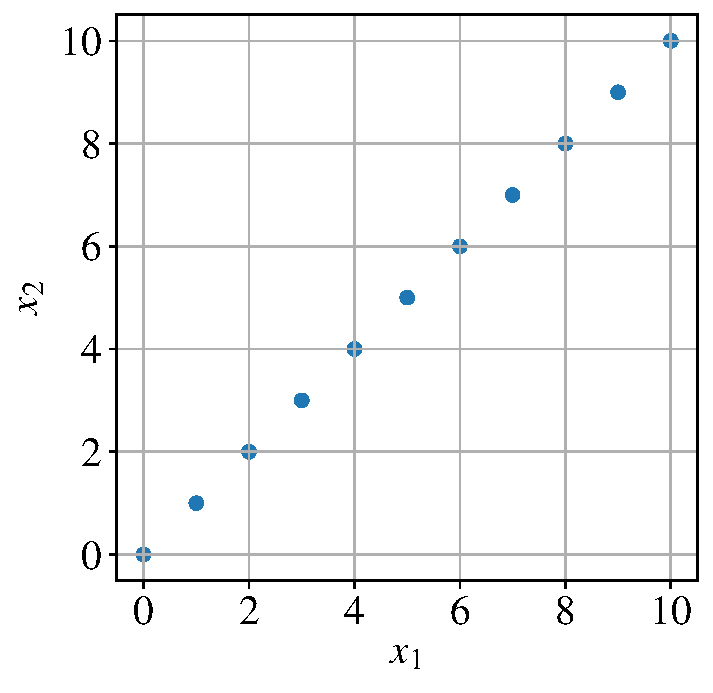
\includegraphics[width=0.4\textwidth]{figures/pca_2d}
  \caption{11 individus représentés par 2 variables $x_1$ et $x_2$.}
  \label{fig:pca_2d}
\end{figure}




\paragraph{Question 2.} Parmi les affirmations ci-dessous, lesquelles sont vraies ? On considère un jeu de données $X \in \RR^{n \times p}$ de $n$ individus en $p$ dimensions.
\begin{itemize}
\item[$\square$] La réduction de dimension relève de l'apprentissage supervisé.
\item[$\square$] La réduction de dimension relève de l'apprentissage non-supervisé.
\item[$\square$] La réduction de dimension facilite la visualisation des données.
\item[$\square$] L'analyse en composantes principales de $X$ permet de créer jusqu'à $n$ nouvelles dimensions. 
\item[$\square$] Les nouvelles variables créées par une analyse en composantes principales sont des combinaisons linéaires des $p$ variables.
\item[$\square$] L'analyse en composantes principales de $X$ s'obtient par une décomposition spectrale de $X$.
\item[$\square$] La sélection de variables consiste à conserver uniquement les variables dont la variance est la plus faible.
\end{itemize}

\section*{Solution}
{%
\noindent
\rotatebox[origin=c]{180}{%
\noindent
\begin{minipage}[t]{\linewidth}
\paragraph{Question 1.} La direction de plus grande variation des données est
la diagonale d'équation $x_1 = x_2$. Ainsi, la première composante principale
est le vecteur directeur de la diagonale, de norme 1, soit donc
$\left(\frac{\sqrt{2}}2, \frac{\sqrt{2}}2\right).$ \newline


\paragraph{Question 2.} 
\begin{itemize}
\item La réduction de dimension peut relever de l'apprentissage supervisé (par
  exemple, l'élimination des variables indépendantes de l'étiquette requièrent
  évidemment une étiquette) ou de l'apprentissage non-supervisé (par
  exemple, l'ACP). Elle est cependant souvent plutôt classée dans
  l'apprentissage non-supervisé car il s'agit d'analyse exploratoire des
  données et non pas d'analyse prédictive, ce qui peut prêter à confusion.
\item[\rlap{$\checkmark$}$\square$] La réduction de dimension facilite la visualisation des données.
\item[$\square$] L'analyse en composantes principales de $X$ permet de créer jusqu'à $n$ nouvelles dimensions. \\
FAUX, elle permet de créer jusqu'à $p$ nouvelles dimensions.
\item[\rlap{$\checkmark$}$\square$] Les nouvelles variables créées par une analyse en composantes principales sont des combinaisons linéaires des $p$ variables.
\item[$\square$] L'analyse en composantes principales de $X$ s'obtient par une décomposition spectrale de $X$.\\
FAUX, il s'agit de la décomposition spectrale de $X^\top X$.
\item[$\square$] La sélection de variables consiste à conserver uniquement les variables dont la variance est la plus faible. \\
FAUX, \textit{une des techniques} de sélection de variables consiste à \textit{éliminer} les variables dont la variance est la plus faible. \\
\end{itemize}
\end{minipage}%
}%



%%% Local Variables:
%%% mode: latex
%%% TeX-master: "../../sdd_2025_poly"
%%% End:






%%% Local Variables:
%%% mode: latex
%%% TeX-master: "../sdd_2025_poly"
%%% End:

\clearpage 

\chapter{Bonnes pratiques}
%-*- coding: utf-8 -*-
\label{chap:pratiques}

\paragraph{Notions :} visualisation de données, représentativité des données,
équité des algorithmes, confidentialité des données, anonymisation,
responsabilité.

\paragraph{Objectifs pédagogiques :} 
\begin{itemize}      
  \setlength{\itemsep}{3pt}
\item S'interroger sur la pertinence d'une analyse de données et la validité
  des conclusions qui en sont tirées.
\end{itemize}

La science des données n'est pas uniquement une discipline technique : comme
souvent en ingénierie, nous ne pouvons pas dissocier les calculs que nous
faisons de la question posée ni de leur utilisation. Ce chapitre n'a pas
vocation à être un cours d'éthique\footnote{L'éthique peut être définie comme
  l'étude de la justification d'ue action à partir de normes, règles juridiques
  ou déontologiques, valeurs morales, intuitions et traditions qui peuvent être
  multiples et contradictoires au sein d'une même société.}, mais à vous donner
quelques points d'entrée pour vous amener à vous poser des questions sur
l'usage de la science des données, de l'apprentissage automatique et de
l'intelligence artificielle. Pour cette raison, vous trouverez plus de liens
externes (cliquables dans la version PDF de ce document) qu'à l'habitude à
travers le texte de ce chapitre, pointant tant vers des publications
scientifiques que des blogs de vulgarisation ou des articles de presse grand
public. N'hésitez pas à poursuivre vos propres lectures sur le sujet.

Nous motiverons ce chapitre par deux citations : la première, attribuée à
Benjamin Disraeli par Mark Twain, ``\textit{There are three kinds of lies:
  lies, damned lies, and statistics}'', et la seconde, attribuée à George
Box, ``\textit{All models are wrong, but some are useful}''.

\section{Visualisation de données}
La façon dont vous choisissez de représenter vos données ou vos résultats a un
impact fort sur le message que vous essayez de faire passer. 

Mi-mai 2020, le Department of Public Health de l'État de Géorgie (États-Unis
d'Amérique) a publié le diagramme en barres de la
figure~\ref{fig:georgia_wtf_barplot}. Regardez bien l'axe des abscisses : le
message vous semble-t-il le même quand les dates sont ordonnées de manière
chronologique, comme sur la figure~\ref{fig:georgia_fixed_barplot} ?

\begin{figure}[h]
  \centering
  \begin{subfigure}[t]{0.47\textwidth}
    \centering
    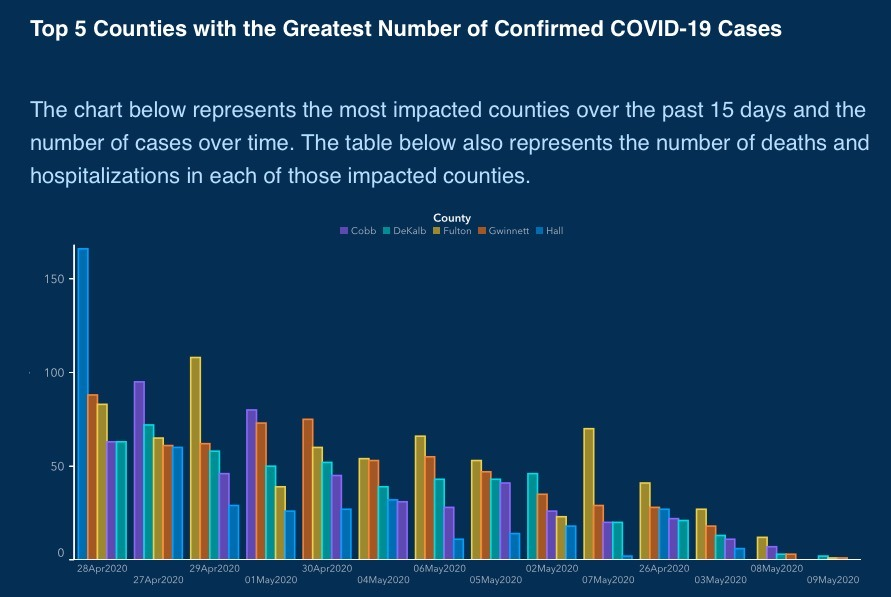
\includegraphics[width=\textwidth]{figures/pratiques/georgia_wtf_barplot}
    \caption{Première version du diagramme en barres.}
    \label{fig:georgia_wtf_barplot}
  \end{subfigure} \hfill
  \begin{subfigure}[t]{0.47\textwidth}
    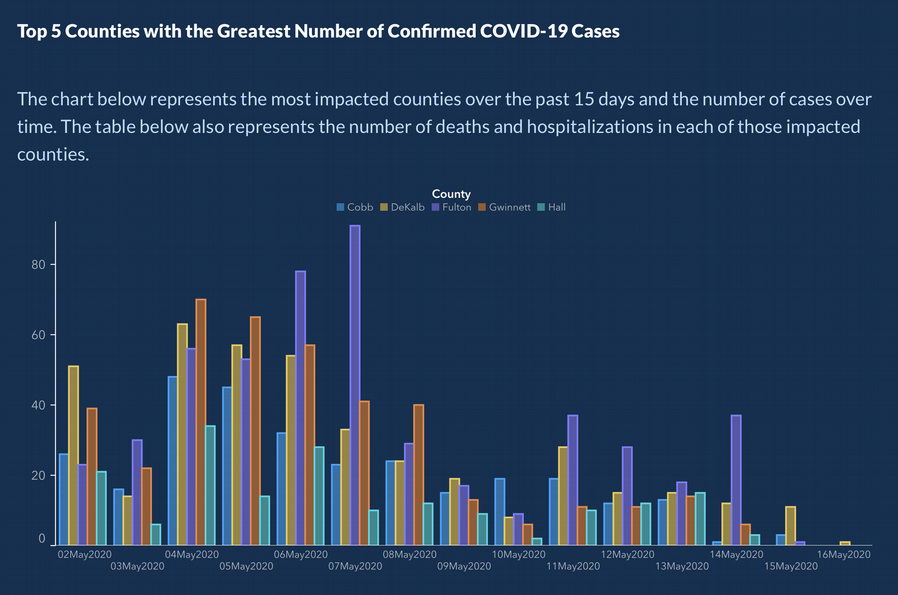
\includegraphics[width=\textwidth]{figures/pratiques/georgia_fixed_barplot}  
    \caption{Deuxième version du diagramme en barres.}
    \label{fig:georgia_fixed_barplot}
  \end{subfigure}  
  \caption{Deux variantes du même diagramme en barres publiées par le
    Department of Public Health de l'État de Géorgie à propos du nombre de cas
    de CoVid19.}
  %\label{fig:georgia_barplot}
\end{figure}

Il est donc très important de vous assurez que vos graphiques soient lisibles
et qu'ils traduisent clairement votre message sans déformer les données. La
visualisation des données, ou \textit{dataviz}, est un champ d'études à part
entière.  Nous nous contenterons ici de citer quelques principes parmi les plus
importants.

\subsection{Des graphiques clairs et lisibles}
Un bon graphique doit pouvoir être compréhensible de manière autonome,
c'est-à-dire sans référence au texte. Pour cela, quelques éléments généraux,
valables bien au-delà de ce cours :
\begin{itemize}
\item Pour être compréhensible, un graphique doit comporter un certain nombre
  d'éléments indispensables à sa compréhension, et en particuilier :
  \begin{itemize}
  \item un titre ;
  \item une légende ;
  \item le nom des axes, l'unité des variables représentées, et l'échelle si
    elle n'est pas linéaire (par exemple, échelle logarithmique).
  \end{itemize}
\item Pour qu'un graphique soit lisible, ses éléments doivent être suffisamment
  grands. Attention en particulier à :
  \begin{itemize}
  \item la taille des textes (légendes, graduations, etc.) ;
  \item la taille des marqueurs et l'épaisseur des traits.
  \end{itemize}
\item Pour être lisible, un graphique ne doit pas comporter d'éléments
  superflus. En particulier, il vaut mieux éviter
  \begin{itemize}
  \item de représenter trop d'informations/éléments à la fois ;
    il est difficile de garder en mémoire plus de 7--10 éléments à la fois
  \item d'utiliser trop de couleurs différentes, surtout si elles ne
    contiennent pas d'information.
  \end{itemize}
\end{itemize}

\subsection{Le choix des axes}
%https://callingbullshit.org/tools/tools_misleading_axes.html 
Le choix des échelles et intervalles d'un graphique a une influence sur son
interprétation.

Pour un diagramme en barres, ne pas faire commencer les axes à 0 peut
artificiellement gonfler les différences entre les différentes barres. Ainsi,
le diagramme de la figure~\ref{fig:bars_start_nonzero} indique que le modèle 4
est bien supérieur aux autres, tandis que celui de la
figure~\ref{fig:bars_start_zero} montre des performances très comparables entre
les différentes méthodes. (Dans ce cas précis, il serait de toute façon
souhaitable de répéter plusieurs fois l'entrainement et l'évaluation, par
exemple avec une validation croisée (que nous verrons
section~\ref{sec:crossval}) et de produire des barres d'erreurs.)
\begin{figure}[h]
  \centering
  \begin{subfigure}[t]{0.47\textwidth}
    \centering
    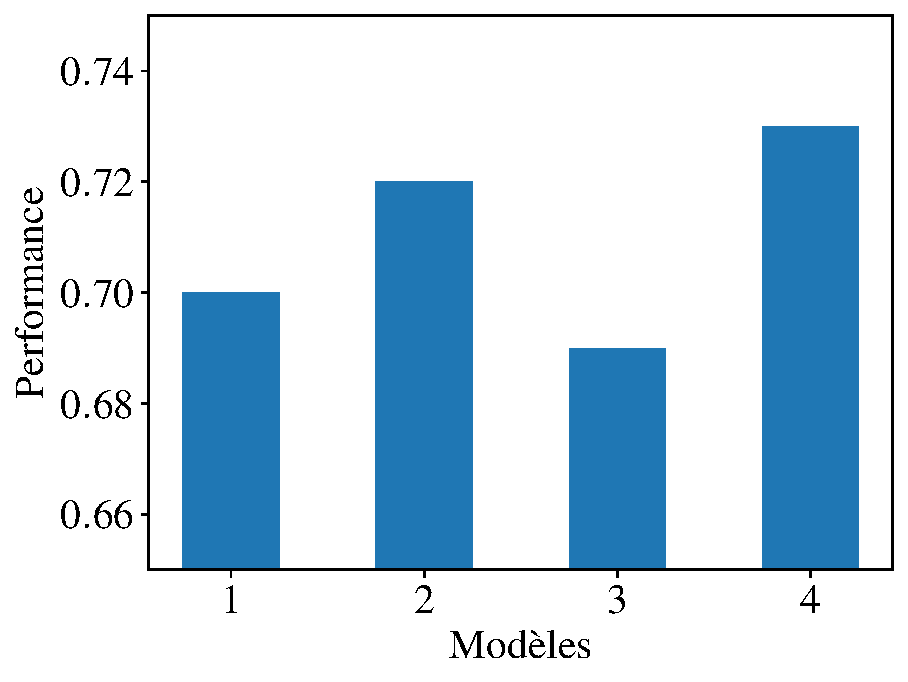
\includegraphics[width=\textwidth]{figures/pratiques/bars_start_nonzero}
    \caption{Axe des ordonnées réduit.}
    \label{fig:bars_start_nonzero}
  \end{subfigure} \hfill
  \begin{subfigure}[t]{0.47\textwidth}
    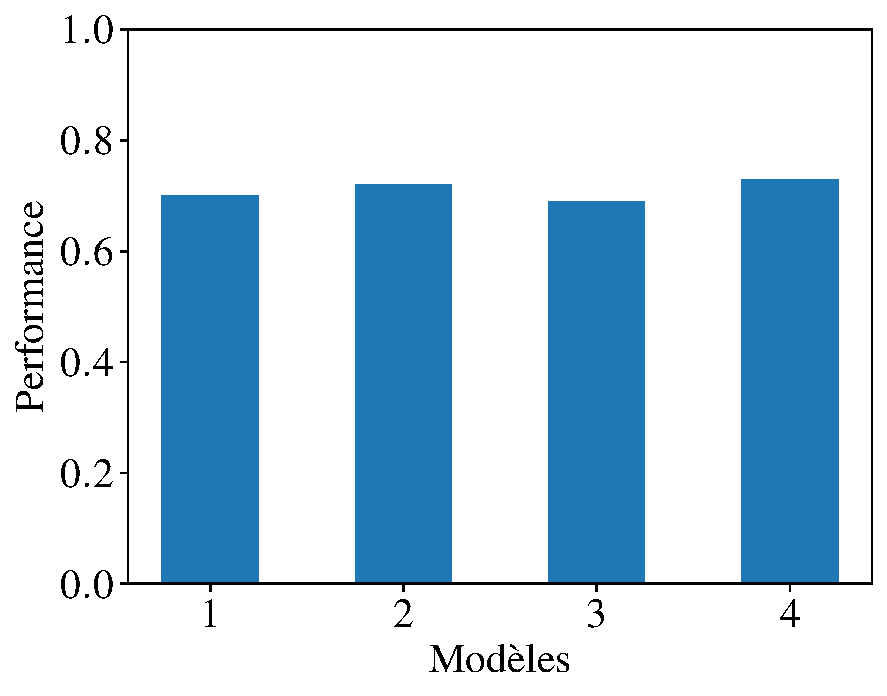
\includegraphics[width=\textwidth]{figures/pratiques/bars_start_zero}  
    \caption{Axe des ordonnées allant de 0 à 1.}
    \label{fig:bars_start_zero}
  \end{subfigure}  
  \caption{Deux façons de présenter la comparaison des performances de 4 modèles.}
  %\label{fig:georgia_barplot}
\end{figure}

À l'inverse, il pourra être préférable pour un diagramme dont le but est non
pas de comparer les valeurs absolues de variables mais plutôt de présenter leur
évolution que l'axe des ordonnées ne commence pas à zéro. Ainsi, la
figure~\ref{fig:line_start_zero} indique une température très stable, tandis
que la figure~\ref{fig:line_start_nonzero} permet de mieux rendre compte des
variations.
\begin{figure}[h]
  \centering
  \begin{subfigure}[t]{0.47\textwidth}
    \centering
    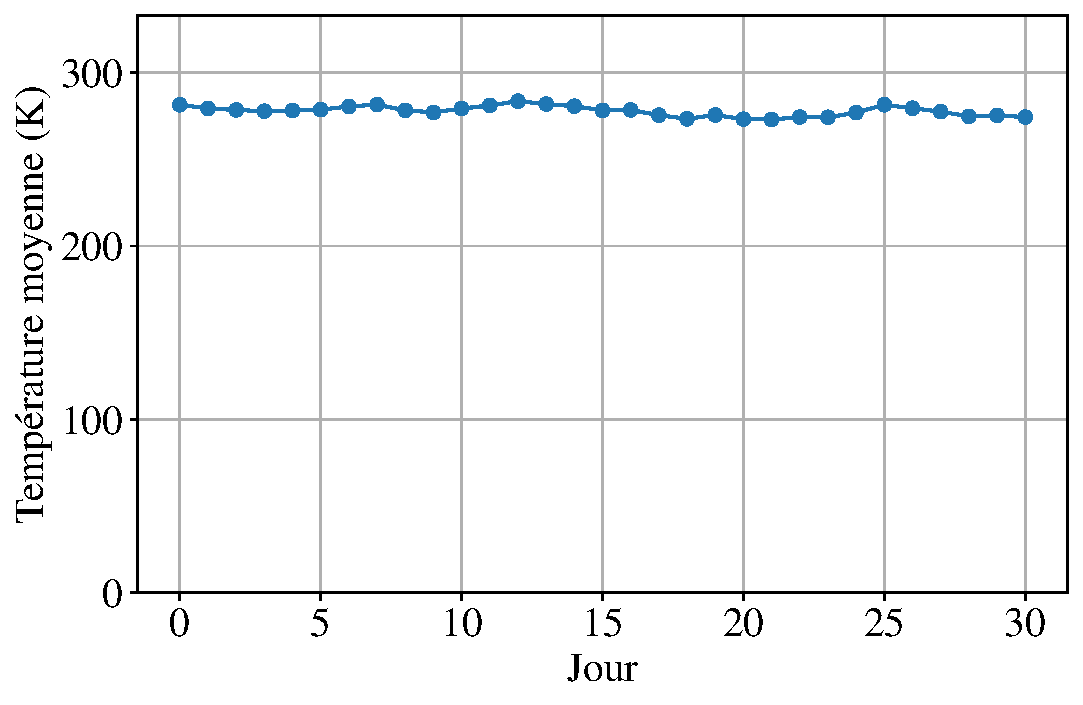
\includegraphics[width=\textwidth]{figures/pratiques/line_start_zero}
    \caption{Axe des ordonnées partant de 0K.}
    \label{fig:line_start_zero}
  \end{subfigure} \hfill
  \begin{subfigure}[t]{0.47\textwidth}
    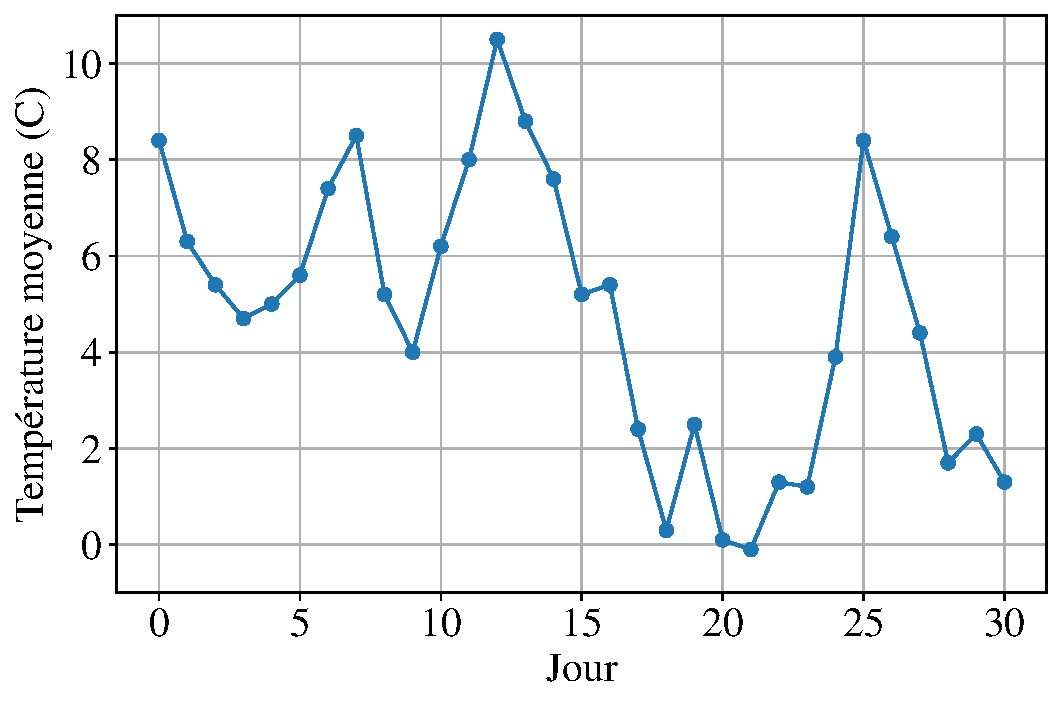
\includegraphics[width=\textwidth]{figures/pratiques/line_start_nonzero}  
    \caption{Axe des ordonnées réduit.}
    \label{fig:line_start_nonzero}
  \end{subfigure}  
  \caption{Deux façons de présenter l'évolution des températures moyenne de la
    table~\ref{tab:meteo_data}.}
  %\label{fig:georgia_barplot}
\end{figure}

\subsection{\textit{Proportional ink} ou principe de l'encre proportionnelle}
%https://callingbullshit.org/tools/tools_proportional_ink.html
De manière générale, il est recommandé, lorsque l'on utilise des surfaces pour
représenter des nombres (par exemple, les rectangles d'un diagramme en barres),
que ces surfaces soient d'aires proportionnelles aux nombres en question. On
retrouve d'ailleurs ici l'idée de commencer les barres d'un diagramme en
barres à 0.

Il faut cependant faire aussi attention à ce que les surfaces en question
soient faciles à comparer visuellement. Un diagramme camembert est ainsi
préférable à un graphique à bulles ; mais un diagramme en barres est
généralement plus lisible qu'un diagramme camembert. La figure~\ref{fig:areas}
l'illustre. Il s'agit d'une variante d'une
\href{https://www.jstor.org/stable/2288400}{expérience
  menée au début des années 1980} et souvent considérée comme fondatrice en
\textit{dataviz}.

Remarquez ici que le diagramme en barres serait encore plus lisible sans couleurs (elles n'apportent rien) et en ordonnant les catégories par proportion.
\begin{figure}[h]
  \centering
  \begin{subfigure}[t]{0.20\textwidth}
    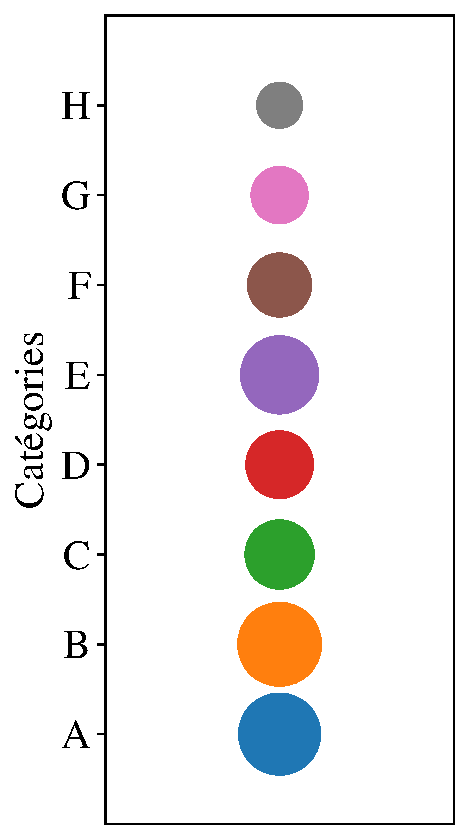
\includegraphics[width=\textwidth]{figures/pratiques/areas_bubbles}  
    \caption{Graphique à bulles.}
    \label{fig:areas_bubbles}
  \end{subfigure}  \hfill
  \begin{subfigure}[t]{0.33\textwidth}
    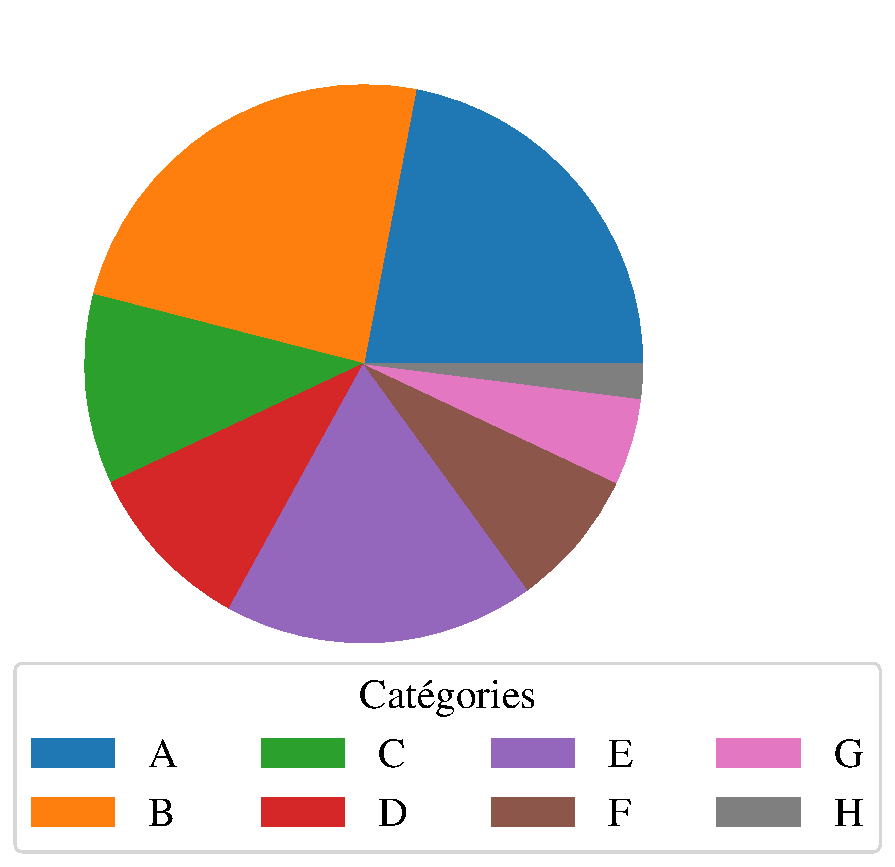
\includegraphics[width=\textwidth]{figures/pratiques/areas_pie}  
    \caption{Diagramme camembert.}
    \label{fig:areas_pie}
  \end{subfigure} \hfill
  \begin{subfigure}[t]{0.33\textwidth}
    \centering
    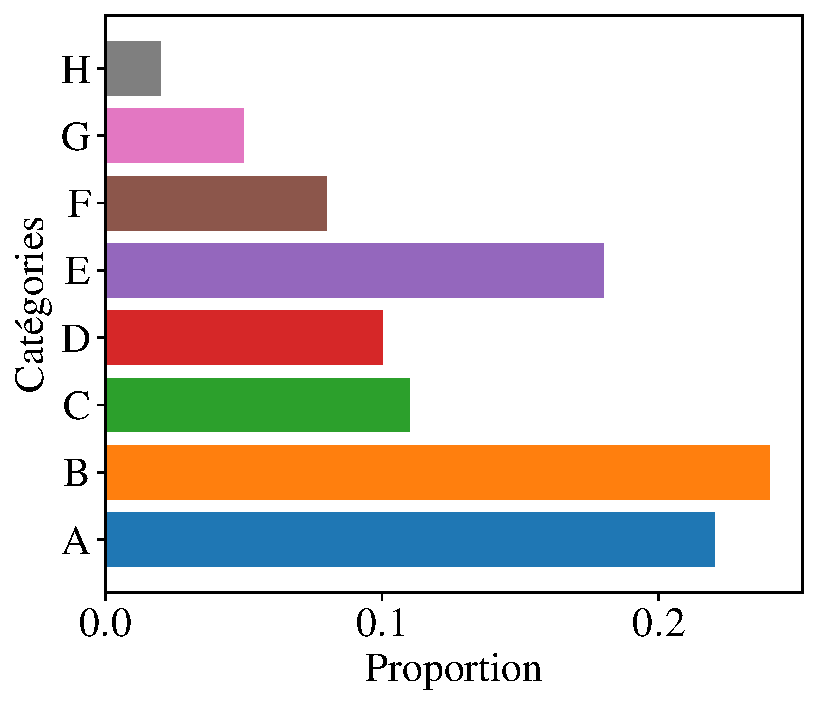
\includegraphics[width=\textwidth]{figures/pratiques/areas_bars}
    \caption{Diagramme en barres.}
    \label{fig:areas_bars}
  \end{subfigure} 
  \caption{Trois façons de représenter les proportions de 8 catégories. Quelle(s) représentation(s) permettent de les classer aisément par ordre croissant ?}
  \label{fig:areas}
\end{figure}

%\subsection{Attention aux résumés}
%https://python-graph-gallery.com/39-hidden-data-under-boxplot/ 


\subsection{Dyschromatopie}
Nous ne percevons pas les couleurs de la même façon. Une forte proportion de la population est atteinte d'une forme ou d'une autre de dyschromatopie, la plus fréquente étant la deutéranopie (incapacité de différencier rouge et vert). 

Pour assurer une accessibilité maximale, utilisez des échelles de couleurs
adaptées. Il est difficile de s'adapter à \textit{toutes} les dyschromatopies ;
néanmoins le cycle par défaut de \texttt{matplotlib} est supposé être
relativement adapté. Pour des \textit{heatmaps}, favoriser les échelles de
couleur \textit{viridis} ou \textit{cividis} (voir
figure~\ref{fig:pca_plot}). Des outils comme \href{https://www.color-blindness.com/coblis-color-blindness-simulator/}{CBLIS} ou \href{https://www.funkify.org}{Funkify} vous permettent de simuler différentes dyschromatopies pour vérifier la lisibilité de vos graphiques.

Vous pouvez aussi augmenter la lisibilité de vos graphiques en utilisant des
indices supplémentaires (épaisseur de trait, hachures, forme des points,
ordonner les légendes dans le même ordre que les courbes, etc.) et en doublant
vos images d'une description textuelle alternative pour les personnes
non-voyantes.


\begin{figure}[h]
  \centering
  \begin{subfigure}[t]{0.30\textwidth}
    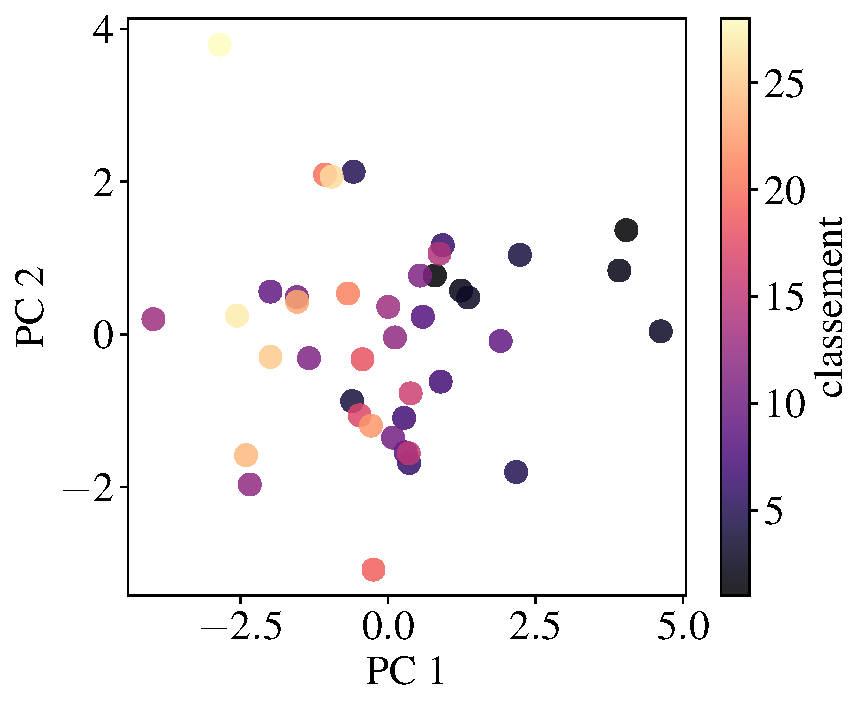
\includegraphics[width=\textwidth]{figures/pratiques/pca_plot_magma}  
    \caption{Magma.}
    \label{fig:pca_plot_magma}
  \end{subfigure}  \hfill
  \begin{subfigure}[t]{0.30\textwidth}
    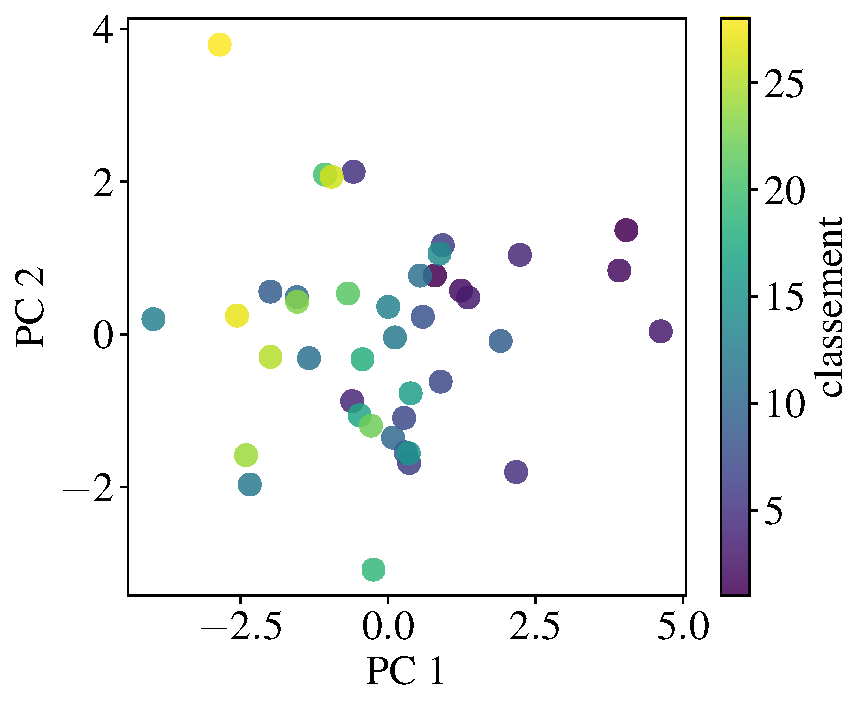
\includegraphics[width=\textwidth]{figures/pratiques/pca_plot_viridis}  
    \caption{Viridis.}
    \label{fig:pca_plot_viridis}
  \end{subfigure} \hfill
  \begin{subfigure}[t]{0.30\textwidth}
    \centering
    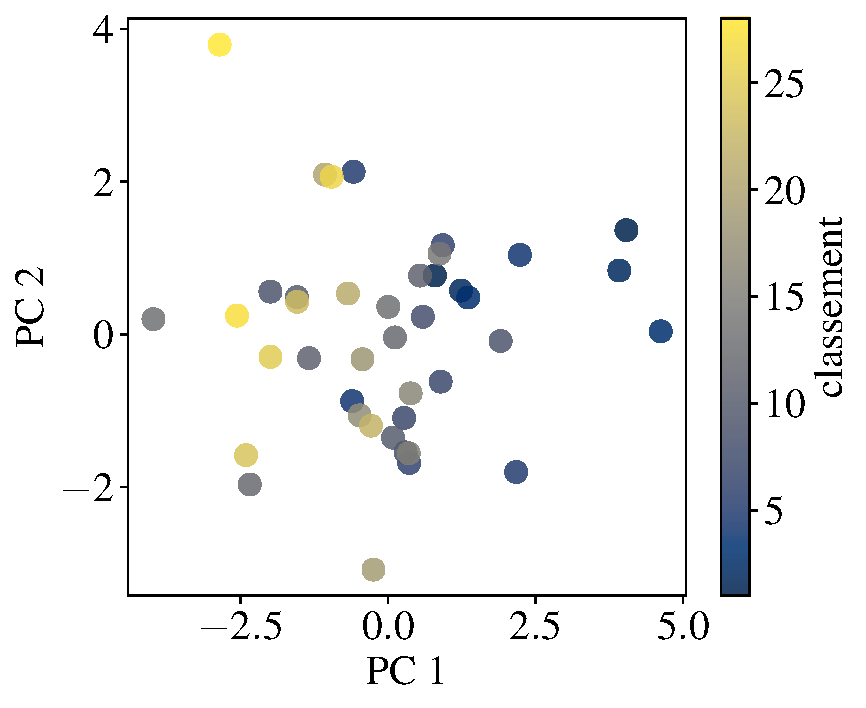
\includegraphics[width=\textwidth]{figures/pratiques/pca_plot_cividis}
    \caption{Cividis.}
    \label{fig:pca_plot_cividis}
  \end{subfigure} 
  \caption{Athlètes de la PC2, représentés selon deux composantes, et colorés
    en fonction de leur classement, selon trois échelles de couleur
    différentes.}
  \label{fig:pca_plot}
\end{figure}

\section{Équité des algorithmes}
Une question importante qui se pose constamment en science des données est
celle de la \textbf{reproduction des biais}. En effet, un modèle appris sur un
jeu de données peut facilement reproduire des biais de ce jeu de données,
qu'ils soient explicites ou implicites.

Un exemple qui revient souvent est celui d'un algorithme de ressources humaines
utilisé par Amazon. Le modèle avait tendance à rejeter les candidatures posées
par des femmes. En effet, il était entraîné sur des données internes à
l'entreprise, dont les recrutements étaient fortement biaisés en faveur des
hommes. Bien que le genre n'ait pas été une variable utilisée pour décrire les
candidatures, le modèle détectait dans le texte des CV des informations
corrélée dans le jeu d'entraînement au rejet d'une candidature mais qui
s'avéraient surtout traduire qu'elle était posée par une femme (éducation dans
un établissement non-mixte réservé aux femmes ; appartenance à une équipe de
sport féminin, etc.).

Ainsi, ce n'est pas parce qu'un modèle statistique est purement mathématique
qu'il est impartial ; en particulier, un modèle ne peut pas être de meilleure
qualité que son jeu d'entraînement. Il faut donc réfléchir à la
\textbf{représentativité} des données : peut-on bien considérer qu'il s'agit
d'un échantillon aléatoire de la population qui nous intéresse, où ne
correspondent-elles qu'à une sous-population spécifique ?

Un autre exemple de reproduction des biais apparait dans une publication de
2016 qui présente un classifieur capable de distinguer criminels de
non-criminels à partir de simples photos. Cependant, les clichés de criminels
étaient des photos administratives prises de face, sans sourire, tandis que les
photos de non-criminels étaient des clichés plus flatteurs : le modèle
 \href{https://callingbullshit.org/case\_studies/case\_study\_criminal\_machine\_learning.html}{détectait
  en fait les sourires}. On retrouve très souvent ce type d'erreurs, dûes à un
\textbf{facteur confondant} : on croit arriver à séparer des images sur leur
contenu alors qu'on utilise principalement leur luminosité ; ou à trouver des
facteurs génétiques influençant le niveau économique, alors que celui-ci est
fortement corrélé dans les données à la couleur de peau ; et ainsi de suite.

Cette étude soulève par ailleurs une question plus large, qui est celle de la
pertinence de ce genre de modèle ; la question de l'équité des algorithmes ne
se ramène pas qu'aux biais dans les données, mais peut aussi concerner leur
pré-traitement, le choix de la question qu'on leur fait résoudre, ou les
décisions prises sur leurs résultats.

La question de l'équité des algorithmes est un sous-domaine important de
l'apprentissage automatique, et se pose d'autant plus que ses applications
s'étendent à des domaines divers et variés touchant de nombreux aspects de nos
sociétés : recrutement mais aussi sécurité, santé, justice, etc. 
C'est le sujet par exemple de l'organisation
\href{https://facctconference.org}{Fairness, Accountability and Transparency in
  Machine Learning}.

Pour autant, il n'y a pas actuellement (et il n'y aura vraisemblablement
jamais) d'outils ou de procédures permettant de garantir cette équité. Il est
ainsi nécessaire de comprendre l'origine possible des biais, ainsi que de
développer des outils pour les mesurer.

Si quelques outils pour l'évaluation d'outils numériques du point de vue
éthique ont vu le jour ces dernières années, comme
\href{http://aequitas.dssg.io/}{Aequitas} aux USA, ceux présentés dans une précédente version de ce poly ont déjà disparu, illustrant les difficultés de ce sujet.

\section{Fiabilité}
Du diagnostic automatisé aux véhicules autonomes, nous avons de plus en plus
envie d'utiliser l'intelligence artificielle, qui présente de nombreuses
opportunités. Mais comment faire confiance aux modèles et algorithmes qui en
sont issus ? Plusieurs questions se posent en plus de celle de l'équité
discutée plus haut.

\paragraph{Vérifiabilité} les systèmes d'IA ont-ils le comportement attendu ?
Les méthodes formelles typiquement utilisées en informatique pour les
programmes utilisés en avionique ne se prêtent guère aux modèles de
l'apprentissage automatique, même si \href{https://formal-paris-saclay.fr/}{de
récents travaux émergent sur le sujet}.

\paragraph{Explicabilité et interprétabilité} Il s'agit aussi de vastes champs
d'étude. Si une régression linéaire est relativement interprétable (cf. PC 3),
des modèles paramétriques plus complexes tels que ceux produits par des réseaux
de neurones artificiels (voir chapitre~\ref{chap:nonlin}) le
sont beaucoup moins. 

\paragraph{Spécification} La description précise du comportement attendu
peut-elle aussi être délicate : quel choix doit faire un véhicule autonome
entre renverser une fillette et emboutir une moto avec deux passagers ? Le MIT
Media Lab propose par exemple \href{http://moralmachine.mit.edu/hl/fr}{La
  Machine Morale}, une plateforme permettant d'explorer divers dilemmes moraux
posés par la prise de décision de machines intelligentes.

\paragraph{Robustesse} Les modèles sont-ils robustes aux attaques ? Depuis
2015, les exemples montrant qu'il est possible d'induire facilement en erreur
un modèle appris par apprentissage automatique s'accumulent. Ces exemples
incluent l'ajout de bruit
indétectable \href{https://arxiv.org/abs/1412.6572}{à l'\oe{}il} ou
\href{https://nicholas.carlini.com/code/audio\_adversarial\_examples}{à
  l'oreille}, la \href{https://arxiv.org/abs/1710.08864}{modification d'un seul
  pixel} d'une image, ou
l'\href{https://towardsdatascience.com/poisoning-attacks-on-machine-learning-1ff247c254db}{empoisonnement}
d'un jeu de données, qui consiste à introduire au moment de l'apprentissage un
faible nombre d'exemples mal étiquetés ou ingénieusement calibrés pour induire
un comportement indésirable.

De même qu'en cryptographie où de nouveaux protocoles émergent pour faire face
à de nouvelles attaques de hackers, l'apprentissage automatique progresse aussi
pour répondre aux attaques
adversariales. \href{http://proceedings.mlr.press/v97/simon-gabriel19a.html}{De
  récents travaux} montrent même qu'en raison du fléau de la dimension, les
attaques adversariales sont inévitables en grande dimension.

\paragraph{Reproductibilité} La démarche scientifique repose sur la
reproductibilité des expériences. Se posent alors la question de la
disponibilité des données, qui peut être limitée pour des raisons de
confidentialité, et celle des \textbf{ressources informatiques} qui peuvent
être nécessaires à entraîner certains modèles. Reproduire des résultats
obtenuse en faisant tourner 800 processeurs graphiques (GPUs) pendant 3
semaines nécessite des ressources financières importantes (on rejoint ici des
questions de coût énergétique et écologique abordées dans la
section~\ref{sec:ecology}).

\paragraph{Responsabilité} Qui est responsable en cas de faillite d'un
système d'IA : l'IA est-elle responsable ? Ou bien la personne qui l'utilise ?
Ou encore celle qui l'a construite ? La question s'est par exemple posée
lorsqu'un véhicule autonome
\href{https://www.nextinpact.com/news/108432-cause-probable-accident-mortel-uber-tout-monde-en-prend-pour-son-grade.htm}{a
  fauché une piétonne} en mars 2018.


\section{Confidentialité des données}
Une grande partie des données utilisées en science des données sont des données
personnelles, c'est-à-dire que les individus qu'elles décrivent sont des
personnes. Nombre d'entre nous s'inquiètent de ce que les données qui nous
concernent, qu'elles soient médicales, de localisation géographique, ou
concernent notre activité numérique, soient utilisées à bon escient.

Les \href{https://risques-tracage.fr/}{discussions autour des applications de traçage de
contacts}
dans la lutte contre la propagation du coronavirus ont bien illustré cette
préoccupation.


En tant que \textit{data scientists}, comment nous assurer que nous ne
compromettons pas la confidentialité des personnes dont nous manipulons les
données ? Deux types de solutions techniques sont possibles.
\paragraph{Dé-identification algorithmique} Il s'agit de s'assurer que l'on ne
puisse pas remonter des données aux individus. Parmi ces techniques,
l'\textbf{anonymisation} consiste à supprimer suffisamment d'informations
identifiantes pour empêcher la réidentification. Ces informations sont dites
\textbf{directement identifiantes} s'il s'agit de caractéristiques personnelles
uniques (nom, numéro de sécurité sociale, numéro de téléphone, etc.) et
\textbf{indirectement identifiantes} si elles permettent d'identifier la
personne de manière unique quand elles sont croisées avec d'autres données
(code postal, date de naissance et lieu de travail pris ensemble peuvent être
indirectement identifiants).  Par contraste, la \textbf{confidentialité
  différentielle}, ou \textit{differential privacy} en anglais cherche plutôt à
garantir que les résultats d'une analyse sur une base de données soient presque
identiques qu'un échantillon soit présent ou non.

\paragraph{Sécurité des bases de données} Cet aspect inclut par exemple le
chiffrement homomorphique permettant d'obtenir les mêmes résultats sur données
chiffrées que non chiffrées, ne laissant ainsi aux \textit{data scientists} que
l'accès aux données chiffrées, des solutions de calcul distribué sécurisées, ou
encore du matériel cryptographique permettant d'exécuter du code sans que les
données ne soient visibles.

En France, la \href{https://www.cnil.fr/}{Commission Nationale de
  l'Informatique et des Libertés (CNIL)} encadre l'utilisation des données
personnelles, qui est notamment encadré par la loi du 14 mai 2018 transposant
le Règlement Général sur la Protection des Données (RGPD) de l'Union
Européenne.


\section{Enjeux écologiques}
\label{sec:ecology}
\href{https://infos.ademe.fr/magazine-avril-2022/faits-et-chiffres/numerique-quel-impact-environnemental/}{Selon
  l'ADEME}, le secteur du numérique est responsable de 2.5\% de l'empreinte carbone de la France, correspondant à 10\% de notre consommation électrique annuelle. Entraîner un réseau de neurones artificiels avec 213 millions de
paramètres peut générer \href{https://arxiv.org/abs/1906.02243}{autant
  d'émissions de CO2 que cinq voitures américaines} pendant toute leur
existence, fabrication comprise. Le
\href{https://mlco2.github.io/impact/}{ML Emissions Calculator}
est un des outils qui accompagnent la prise de conscience de l'impact
environnemental de la science des données. Ces enjeux deviennent d'autant plus importants que l'on développe de très grands modèles, notamment en traitement automatisé du langage ; deux exemples récents de travaux sur ces questions sont \href{https://arxiv.org/abs/2304.03271}{\textit{Making AI less thirsty: uncovering and addressing the secret water footprint of AI models}}, qui s'intéresse à la consommation en eau des modèles, et \href{https://arxiv.org/abs/2211.02001}{\textit{Estimating the Carbon Footprint of BLOOM}}, qui essaie d'estimer l'empreinte carbone d'un modèle de langage à 176 milliards de paramètres.

\begin{plusloin}
\item Des ouvrages entiers ont étés écrits sur la \textit{dataviz}, par exemple \href{https://clauswilke.com/dataviz/}{\textit{Fundamentals of Data Vizualization} de Claus O. Wilke}, le travail d'\href{https://www.edwardtufte.com/tufte/}{Edward Tufte}, \href{https://informationisbeautiful.net/}{\textit{Information is Beautiful} de David McCandless}, ou encore \href{https://github.com/rougier/scientific-visualization-book}{\textit{Scientific Visualization} de Nicolas Rougier}.
% \item \href{https://hippocrate.tech/}{Le Serment d'Hippocrate pour Data Scientist} de Data for Good.
\item La représentativité est une question qui revient dans de nombreux
  domaines de l'ingénierie. Les exemples sont nombreux, des
  \href{https://www.huffingtonpost.fr/2017/08/19/ce-distributeur-automatique-ne-distribue-pas-de-savon-aux-mains\_a\_23152387/}{distributeurs
    de savon qui ne détectent que les peaux claires} à tous les
  objets plutôt adaptés aux hommes recensés par Caroline Criado
  Perez dans
  \href{https://www.liberation.fr/france/2020/03/06/les-femmes-invisibles-dans-un-monde-cree-pour-les-hommes\_1780895}{\textit{Invisible
      Women}}.
  \item Un épisode de La Méthode Scientifique  intitulé \href{https://april.org/ethique-numerique-des-datas-sous-serment-emission-la-methode-scientifique}{\textit{Éthique numérique, des data sous
    serment}}.
  \item \href{https://fairmlbook.org/}{\textit{Fairness and Machine Learning}} de Solon
    Barocas, Moritz Hardt and Arvind Narayanan.
  \item À propos de \href{https://www.latribune.fr/supplement/ceux-qui-transforment-la-france/la-justice-predictive-nouvel-outil-pour-les-professionnels-du-droit-837752.html}{justice prédictive}, l'article \href{https://www.dalloz-actualite.fr/flash/justice-et-intelligence-artificielle-preparer-demain-episode-i}{Justice
        et intelligence artificielle : préparer demain} dans Dalloz Actualité.
  \item \href{https://hbr.org/2013/04/the-hidden-biases-in-big-data}{\textit{The Hidden Biases in Big Data}}, Kate Crawford, HBR, April 2013. 
  \item \href{https://salil.seas.harvard.edu/files/salil/files/differential_privacy_primer_nontechnical_audience.pdf}{\textit{Differential privacy: A primer for a non-technical audience}}, A. Wood et al., Vanderbilt Journal of \\Entertainment and Technology Law.
  \item Le \href{https://ethics-of-ai.mooc.fi/start}{cours d'éthique de l'IA de l'Université d'Helsinki}
\end{plusloin}



%%% Local Variables:
%%% mode: latex
%%% TeX-master: "../sdd_2025_poly"
%%% End:



\part{Apprentissage supervisé}
\chapter{Minimisation du risque empirique}
%-*- coding: utf-8 -*-
\label{chap:erm}

\paragraph{Notions :} classification, régression, espace des hypothèses,
minimisation du risque empirique, modèles paramétriques
linéaires, moindres carrés
\paragraph{Objectifs pédagogiques :} 
\begin{itemize}      
  \setlength{\itemsep}{3pt}
\item Formaliser un problème d'apprentissage supervisé.
\item Décrire l'espace des hypothèses dans le cas d'un modèle paramétrique.
\item Prouver l'équivalence entre maximisation de la vraisemblance et
  minimisation du risque empirique dans le cas gaussien. $\bullet$ 
\item Mettre en \oe{}uvre une régression linéaire.
\end{itemize}

Nous nous intéressons maintenant aux problèmes d'apprentissage \textbf{supervisé}
: il s'agit de développer des algorithmes qui soient capables d'apprendre des
modèles \textbf{prédictifs}. À partir d'exemples étiquetés, ces modèles seront
capables de prédire l'étiquette de nouveaux objets. Le but de ce chapitre est
de développer les concepts généraux qui nous permettent de formaliser ce type
de problèmes.

\section{Formalisation d'un problème d'apprentissage supervisé}
\label{sec:sup_learn}
Nous supposons maintenant disposer non seulement d'une matrice
$X \in \RRnp$ décrivant $n$ individus en $p$ dimensions, mais aussi
de $n$ \textbf{étiquettes} $\{y^1, y^2, \dots, y^n\}$. Chaque étiquette $y^i$
appartient à un espace $\YY.$ Dans ce cours, nous allons considérer deux cas
particuliers pour $\YY:$
\begin{itemize}
\item $\YY = \RR :$ on parle d'un problème de \textbf{régression} ;
\item $\YY = \zo :$ on parle d'un problème de \textbf{classification
    binaire}, et les observations dont l'étiquette vaut $0$ sont appelées
  \textbf{négatives} tandis que celles dont l'étiquette vaut $1$ sont appelées
  \textbf{positives}. Dans certains cas, il sera mathématiquement plus simple
  d'utiliser $\YY = \mopo$.
\end{itemize}

La matrice $X \in \RRnp$ telle que $X_{ij} = x^i_j$ est la $j$-ème
variable du $i$-ème individu est appelée \textbf{matrice de données} ou
\textbf{matrice de design}. 

On peut aussi choisir de représenter chaque individu et son étiquette par le
couple $(\xx^i, y^i) \in \RR^{p} \times \YY.$ L'ensemble
$\DD = \{(\xx^i, y^i)\}_{i=1, \dots, n}$ forme alors le \textbf{jeu d'apprentissage}.

Le machine learning étant issu de plusieurs disciplines et champs
d'applications, on trouvera plusieurs noms pour les mêmes objets.  Ainsi les
variables sont aussi appelées \textbf{descripteurs}, \textbf{attributs},
\textbf{prédicteurs}, ou \textbf{caractéristiques} (en anglais,
\textit{variables, descriptors, attributes, predictors} ou encore
\textit{features}).  Les \textbf{individus}, ou \textbf{observations} sont
aussi appelées \textbf{exemples}, \textbf{échantillons} ou \textbf{points du
  jeu de données} (en anglais, \textit{samples} ou \textit{data
  points}). Enfin, les étiquettes sont aussi appelées \textbf{variables cibles}
(en anglais, \textit{labels, targets} ou \textit{outcomes}).

% Ces concepts sont illustrés sur la figure~\ref{fig:suplearning}.

% \begin{figure}[h]
%   \centering
%   \includegraphics[width=0.7\textwidth]{figures/erm/suplearning}
%   \caption{Les données d'un problème d'apprentissage supervisé sont organisées
%     en une matrice de design et un vecteur d'étiquettes. Les observations sont
%     représentées par leurs variables explicatives.}
%   \label{fig:suplearning}
% \end{figure}

Le but de l'apprentissage supervisé est alors de trouver une fonction
$f: \RR^p \to \YY$ telle que $f(\xx) \approx y,$ qui s'applique non
seulement aux $n$ individus observés, mais plus généralement à tous les
individus d'une population à laquelle on suppose que ces $n$ individus
appartiennent. C'est cette fonction $f$ qui est le \textbf{modèle prédictif}
appris. Un \textbf{algorithme d'apprentissage supervisé} utilise le jeu de
données $\DD$ pour déterminer $f$.

Plus formellement, supposons que les couples $(\xx^i, y^i)$ soient les
réalisations de $n$ vecteurs aléatoires de même loi qu'un couple de variables
aléatoire $(X, Y)$, $X$ étant un vecteur aléatoire à $p$ dimensions et $Y$ une
variable aléatoire réelle à valeurs dans $\YY$. Supposons de plus qu'il existe
une fonction $\Phi \colon \RR^p \to \YY$ et une variable aléatoire réelle
$\epsilon$ telle que
  \begin{equation}
  Y = \Phi(X) + \epsilon,
  \label{eq:probabilistic_ml}
\end{equation}
$\epsilon$ représentant un \textbf{bruit}.
Ce bruit peut être causé
\begin{itemize}
\item par des {\it erreurs de mesure} dues à la faillibilité des capteurs
  utilisés pour mesurer les variables par lesquelles on représente nos
  données, ou à la faillibilité des personnes qui ont entré ces
  mesures dans une base de données ;
\item par des {\it erreurs d'étiquetage} (souvent appelés {\it teacher's noise}
  en anglais) dues à la faillibilité des personnes qui ont étiqueté
  les données ;
\item enfin, parce que les variables mesurées ne suffisent pas à modéliser le
  phénomène qui nous intéresse, soit qu'on ne les connaisse pas, soit
  qu'elles soient coûteuses à mesurer.
\end{itemize}
Notre but est d'approcher $\Phi$ par $f$.

Dans le cas d'un problème de classification, le modèle prédictif peut prendre
directement la forme d'une fonction $f$ à valeurs dans $\zo$, ou utiliser
une fonction intermédiaire $g$ à valeurs réelles, qui associe à une observation
un score d'autant plus élevé qu'elle est susceptible d'être positive. Ce score
peut par exemple être la probabilité que cette observation appartienne à la
classe positive. On obtient alors $f$ en \textbf{seuillant} $g$ ; $g$ est
appelée \textbf{fonction de décision} \footnote{Dans la librairie
  \texttt{scikit-learn}, on fera ainsi attention à la distinction entre les
  méthodes \texttt{predict} et \texttt{predict\_proba}.}.

\begin{exemple}
  \paragraph{Filtrage de spam.} On peut poser le filtrage de spam comme un
  problème de classification binaire. Les individus sont des emails. Leur
  étiquette est binaire (positive pour « spam » et négative pour « non-spam
  »). Les $p$ variables représentant un email peuvent être définies comme le
  nombre d'occurrences, pour $p$ mots, de chacun de ces mots dans l'email ($p$
  est ainsi la taille d'un dictionnaire pré-défini)\footnote{C'est ce qu'on
    appelle une représentation \textit{bag-of-words}}. Étant donné un jeu de
  données de $n$ emails étiquetés, un algorithme d'apprentissage retourne une
  fonction $f$ qui, à tout email représenté par un vecteur de $\RR^p$ (en fait,
  $\NN^p$), associe une étiquette $0$ ou $1$. Ce modèle
  $f: \RR^p \to \zo$ peut être obtenu en seuillant une fonction de
  décision $g: \RR^p \to \RR$.

  Le bruit peut être dû aux causes suivantes :
  \begin{itemize}
  \item Des erreurs de mesures peuvent être causées par des fautes
    d'orthographe (volontaires ou non) qui empêchent de comptabiliser certains
    mots.
  \item Des erreurs d'étiquetage peuvent arriver quand une personne marque par
    erreur comme courrier indésirable un email qui ne l'était pas, ou,
    inversement, laisse dans sa boîte mail ou supprime sans étiqueter comme tel
    un email indésirable.
  \item Enfin, notre représentation est limitée, en particulier parce qu'elle
    ne considère pas l'ordre des mots. Nous ne disposons pas de suffisamment
    d'information pour classifier les emails aussi efficacement qu'un humain.
  \end{itemize}
\end{exemple}


\paragraph{Remarque.} Les notions développées jusqu'à la fin de la
section~\ref{sec:losses} peuvent l'être en remplaçant $\RR^p$ par un espace
quelconque $\XX$.


\section{Espace des hypothèses}
Pour poser un problème d'apprentissage supervisé, il nous faut décider du
type de modèles que nous allons considérer. 

On appelle \textbf{espace des hypothèses} l'espace de fonctions $\FF$, qui est
un sous-espace de toutes les fonctions de $\RR^p \to \YY$ décrivant les
modèles que nous allons considérer. Cet espace est choisi en
fonction de nos {\it convictions} par rapport au problème, ainsi que de
considérations pratiques sur notre capacité à trouver facilement un « bon »
modèle dans $\FF$.

Le choix de l'espace des hypothèses est fondamental.  En effet, si cet espace
ne contient pas le \og bon \fg~modèle, il sera impossible de trouver une bonne
fonction de décision.  Cependant, si l'espace est trop générique, il sera plus
difficile et intensif en temps de calcul d'y trouver un bon modèle.
  

\begin{exemple}
  Dans l'exemple de la figure~\ref{fig:simple_classif_pb}, on pourra décider de
  se restreindre à des discriminants qui soient des ellipses à axes parallèles
  aux axes de coordonnées.  Ainsi, l'espace des hypothèses sera
  \begin{equation}
    \FF = \{ \xx \mapsto \alpha (x_1-a)^2 + \beta (x_2-b)^2 - 1 \; ; (\alpha, \beta, a, b) \in \RR^4\}.
    \label{eq:hypothesis_space_ellipsis}
  \end{equation}

  Dans cet espace, il semble possible de trouver un modèle $f$ qui sépare les
  positifs des négatifs. Si nous avions choisi comme espace des hypothèses
  l'ensemble des fonctions linéaires de $\RR^2$ dans $\RR$, ce ne serait pas
  possible.
\end{exemple}
\begin{figure}[h]
  \centering
  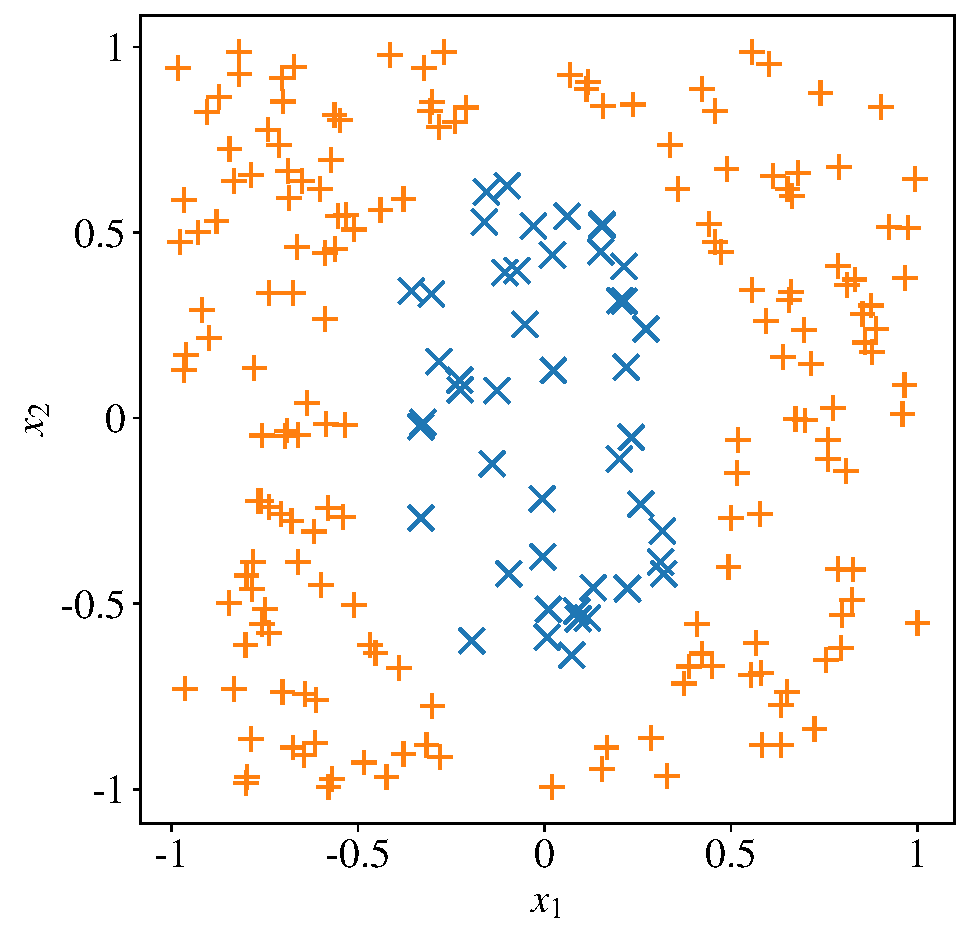
\includegraphics[width=0.45\textwidth]{figures/erm/simple_classif}
  \caption{Les exemples positifs (+) et négatifs (x) semblent être séparables
    par une ellipse.}
  \label{fig:simple_classif_pb}
\end{figure}

La tâche d'apprentissage supervisé consiste à déterminer une hypothèse
$f \in \FF$ qui approche au mieux la fonction cible $\Phi$ (voir
équation~\eqref{eq:probabilistic_ml}). Pour réaliser une telle tâche, nous
allons développer dans les sections suivantes deux outils supplémentaires :
\begin{enumerate}
\item Une façon de \textbf{quantifier la qualité d'une hypothèse}, afin de
  pouvoir déterminer si une hypothèse satisfaisante (voire optimale) a été
  trouvée.  Pour cela, nous allons définir la notion de \textbf{fonction de
    coût}.
\item Une façon de \textbf{chercher une hypothèse optimale} dans $\FF$.  Les
  algorithmes d'apprentissage supervisé que nous allons étudier ont pour but de
  trouver dans $\FF$ l'hypothèse optimale au sens de la fonction de coût. Selon
  les cas, et en particulier selon le choix de $\FF,$ cette recherche sera
  exacte ou approchée.
\end{enumerate}

\section{Minimisation du risque empirique}
\label{sec:mre}
Résoudre un problème d'apprentissage supervisé revient à trouver une fonction
$f \in \FF$ dont les prédictions soient les plus proches possibles des
véritables étiquettes, sur tout l'espace $\RR^p$. On utilise pour formaliser cela
la notion de \textbf{fonction de coût} :

Une \textbf{fonction de coût} $L: \YY \times \YY \to \RR$, 
aussi appelée \textbf{fonction de perte} ou \textbf{fonction d'erreur}
(en anglais : {\it cost function} ou {\it loss function})
est une fonction utilisée pour quantifier la qualité d'une prédiction : 
$L(y, f(\xx))$ est d'autant plus grande que l'étiquette $f(\xx)$ est éloignée de
la vraie valeur $y$.

Étant donnée une fonction de coût $L$, nous cherchons donc $f$ qui minimise ce
coût sur l'ensemble des valeurs possibles de $\xx \in \RR^p$, ce qui est
formalisé par la notion de \textbf{risque.} Nous supposons que les couples
$(\xx^i, y^i)$ sont les réalisations de $n$ vecteurs aléatoires de même loi
qu'un couple de variables aléatoire $(X, Y).$

Dans le cadre d'un problème d'apprentissage supervisé, on appelle
\textbf{risque} d'un modèle $h$ l'espérance de son coût :
\begin{equation}
  \label{eq:risque}
  \Rcal(h) = \EE(L(Y, f(X))).
\end{equation}

Nous cherchons donc un modèle $f$ tel que 
\begin{equation}
  \label{eq:risk_minimization}
  f \in \argmin_{h \in \FF} \EE(L(Y, h(X))).
\end{equation}
Ce problème est généralement insoluble sans plus d'hypothèses : nous ne
connaissons que $n$ réalisations du couple $(X, Y)$.  On approchera donc le
risque par son estimation sur ces réalisations.

On appelle \textbf{risque empirique} de $h$ l'estimée du risque de $h$ défini par
\begin{equation}
  \label{eq:empirical_risk}
  R_n(h) = \frac{1}{n} \sum_{i=1}^n L(y^i, h(\xx^i)).
\end{equation}

On appelle donc modèle obtenu par \textbf{minimisation du risque empirique} une
fonction
\begin{equation}
  \label{eq:erm}
  f \in \argmin_{h \in \FF} \frac{1}{n} \sum_{i=1}^n L(y^i, h(\xx^i)).
\end{equation}

Selon le choix de $\FF$ et $L$, l'équation~\ref{eq:erm} peut avoir une solution
analytique explicite. Cela ne sera pas souvent le cas ; cependant on choisira
souvent une fonction de coût convexe afin de résoudre plus facilement ce
problème d'optimisation.

La minimisation du risque empirique est généralement un problème {\it mal
  posé}, c'est-à-dire qu'il n'admet pas une solution unique dépendant de façon
continue de conditions initiales. Il se peut par exemple qu'un nombre infini
de solutions minimise le risque empirique à zéro (voir
figure~\ref{fig:multiple_solutions}).

\begin{figure}[h]
  \centering
  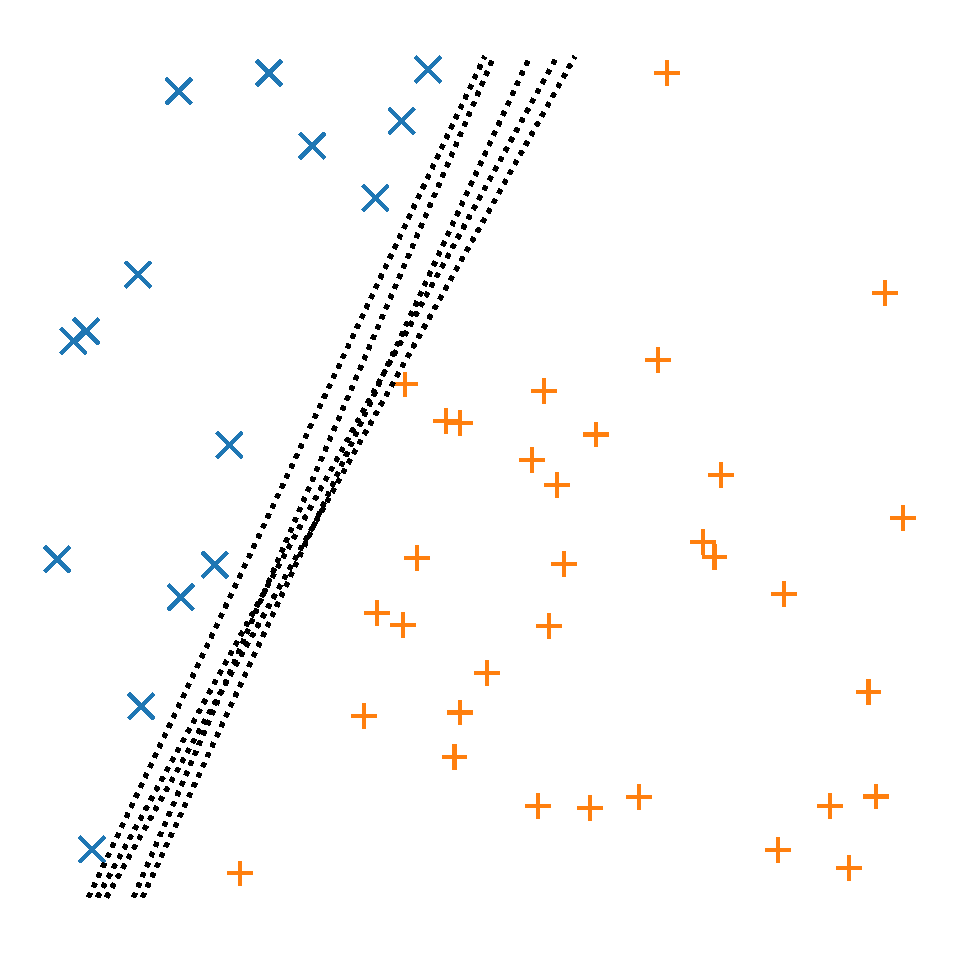
\includegraphics[width=0.4\textwidth]{figures/erm/multiple_solutions}
  \caption{Une infinité de droites séparent parfaitement les points positifs
    (+) des points négatifs (x). Chacune d'entre elles a un risque empirique
    nul.}
  \label{fig:multiple_solutions}
\end{figure}


\paragraph{Convergence} La loi des grands nombres nous garantit que le risque
empirique d'un modèle $h \in \FF$ converge vers le risque quand la taille de
l'échantillon tend vers l'infini :
\begin{equation}
  \label{eq:risk_cvg}
  R_n(h) \xrightarrow[n \to \infty]{} \Rcal(h).
\end{equation}
Cela ne suffit cependant pas à garantir que le minimum du risque empirique
$\min_{h \in \FF} R_n(h)$ converge vers le minimum du risque
$\min_{h \in \FF} \Rcal(h)$. En effet, si $\FF$ est l'espace des fonctions
mesurables, le minimiseur de $R_n(h)$ vaut généralement $0$, ce qui n'est pas
le cas de $\Rcal(h).$ \textbf{Il n'y a donc aucune garantie qu'un modèle qui
  minimise le risque empirique minimise le risque.} C'est une remarque très
importante car elle signifie que le fait qu'un modèle minimise l'erreur sur nos
$n$ observations ne donne aucune garantie quant à sa performance sur d'autres
observations. Nous reviendrons sur ce sujet lors du prochain chapitre, en abordant
les notions de généralisation et de surapprentissage.

La convergence de la minimisation du risque empirique dépend de $\FF$. L'étude
de cette convergence est l'un des principaux éléments de la théorie de
l'apprentissage de Vapnik-Chervonenkis, qui dépasse largement le cadre de ce
cours.


\section{Fonctions de coût}
\label{sec:losses}
Il existe de nombreuses fonctions de coût. Le choix d'une fonction de coût
dépend d'une part du problème en lui-même, autrement dit de ce que l'on trouve
pertinent pour le cas pratique considéré, et d'autre part de considérations
pratiques : peut-on ensuite résoudre le problème d'optimisation qui résulte de
ce choix de façon suffisamment exacte et rapide~?
Cette section présente quelques-unes des fonctions de coût les plus utilisées.

\subsection{Coût 0/1 (classification)}
Dans le cas d'une fonction $f$ à valeurs discrètes, on appelle \textbf{fonction
  de coût 0/1}, ou {\it 0/1 loss}, la fonction suivante :
\begin{align*}
  L_{0/1}\colon\YY \times \YY & \to \RR \\
  y, f(\xx) & \mapsto
              \begin{cases}
                1 & \mbox{ si } f(\xx) \neq y \\
                0 & \mbox{ sinon.}
              \end{cases}
\end{align*}
Le risque empirique d'un modèle $h$ sur un jeu de données est alors le nombre
d'erreurs de prédiction sur ce jeu de données.

\subsection{Coût logistique et entropie croisée (classification binaire)}
Considérons maintenant que $f$ est une fonction de décision à valeurs réelles.
\label{sec:logistic_loss}
On appelle \textbf{fonction de coût logistique}, ou {\it logistic loss}, la
fonction suivante :
\begin{equation}
  \begin{split}
  L_{\log}\colon\mopo \times \RR & \to \RR \\ 
  y, f(\xx) & \mapsto \ln \left( 1 + \exp(-y f(\xx))\right). 
\end{split}
  \label{eq:logistic_loss}
\end{equation}

Si $f$ est à valeurs dans $]0, 1[$, en particulier si $f(\xx)$ est la
probabilité que $\xx$ appartienne à la classe positive, % cette fonction de coût
% est équivalente à
on utilise plutôt
l'\textbf{entropie croisée}, définie pour $\YY = \zo$.

\label{sec:cross_entropy}
On appelle \textbf{entropie croisée}, ou {\it cross-entropy},
la fonction suivante :
\begin{equation}
  \begin{split}
    L_H \colon \zo \times ]0, 1[ & \to \RR \\
    y, f(\xx) & \mapsto - y \ln f(\xx) - (1-y) \ln(1-f(\xx)).
  \end{split}
  \label{eq:cross_entropy}
\end{equation}

\paragraph{Remarque} On peut transformer une fonction $f$ à valeurs dans $\RR$
en une fonction $h$ à valeurs dans $]0, 1[$ en la composant par la
\textbf{fonction sigmoïde,} aussi appelée \textbf{fonction logistique,} définie
par
\begin{equation}
  \label{eq:sigmoide}
  \begin{split}
    \sigma \colon \RR & \to ]0, 1[ \\
    u & \mapsto \frac1{1 + e^{-u}}.
  \end{split}
\end{equation}
Dans ce cas, la fonction de coût logistique appliquée à $f$ est équivalente à
l'entropie croisée appliquée à $h = \sigma \circ f$ :
\[
  L_H(y, h(\xx)) = L_{\log} (2y-1, f(\xx))
\]

La figure~\ref{fig:logistic_loss} illustre la valeur de la fonction de coût
logistique en fonction de l'étiquette $y$ de l'individu $\xx$ et de la valeur
de la fonction de décision $f(\xx) \in ]0, 1[.$ 

\begin{figure}[h]
  \centering
  \begin{subfigure}[t]{0.43\textwidth}
    \centering
    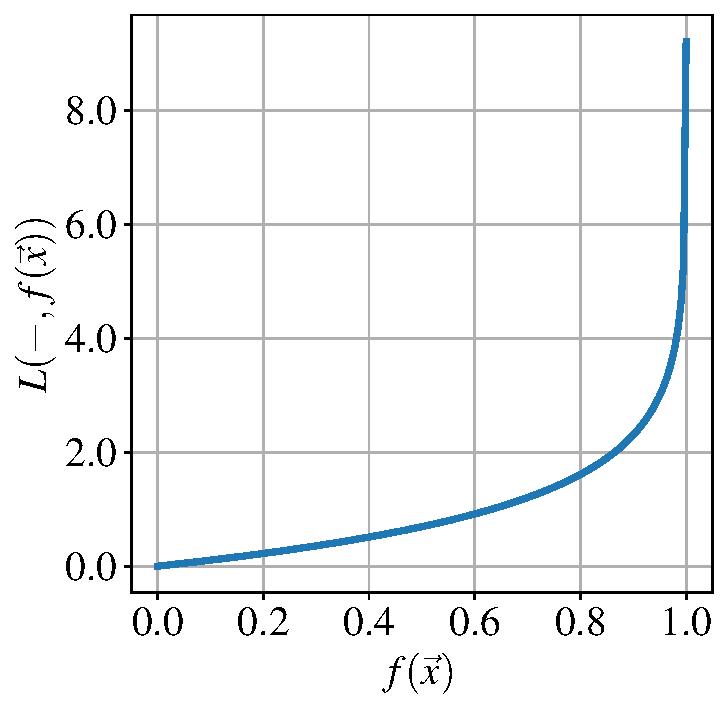
\includegraphics[width=\textwidth]{figures/erm/logistic_loss_neg}
    \caption{Entropie croisée pour un individu d'étiquette négative, en
      fonction de la valeur de la fonction de décision. Cette perte est
      d'autant plus grande que la fonction de décision est proche de $1$.}
    \label{fig:logistic_loss_neg}
  \end{subfigure} \hfill
  \begin{subfigure}[t]{0.43\textwidth}
    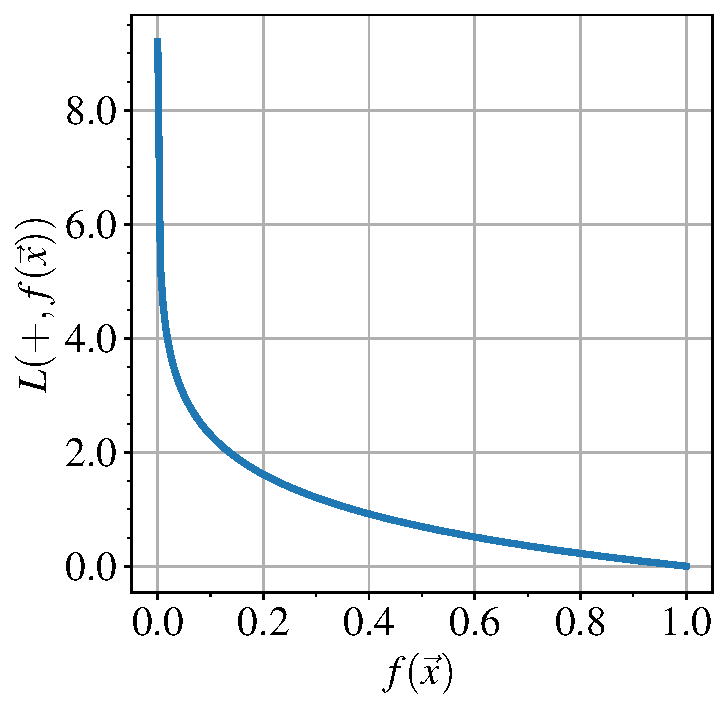
\includegraphics[width=\textwidth]{figures/erm/logistic_loss_pos}  
    \caption{Entropie croisée pour un individu d'étiquette positive, en
      fonction de la valeur de la fonction de décision. Cette perte est
      d'autant plus grande que la fonction de décision est proche de $0$.}
    \label{fig:logistic_loss_pos}
  \end{subfigure}
  \caption{Valeur de l'entropie croisée en fonction de la valeur de la fonction de décision.}
  \label{fig:logistic_loss}
\end{figure}


\paragraph{Pourquoi « entropie croisée » ? $\bullet\bullet$ } 
L'entropie croisée est issue de la théorie de l'information, d'où son nom. En
considérant que la véritable classe d'une observation est modélisée par une
distribution $Q$, et sa classe prédite est modélisée par une distribution $P$,
nous allons chercher à modéliser $P$ de sorte qu'elle soit la plus proche
possible de $Q$. On utilise pour cela la divergence de Kullback-Leibler,
définie par :
\begin{align*}
  \text{KL}(Q||P) & = \sum_{c=0, 1} Q(Y=c|X) \ln \frac{Q(Y=c|X)}{P(Y=c|X)} \\
           & = - \sum_{c=0, 1} Q(Y=c|X) \ln P(Y=c|X) + 
             \sum_{c=0, 1} Q(Y=c|X) \ln Q(Y=c|X).
\end{align*}
Comme $Q(Y=c|X)$ vaut soit $0$ ($c$ n'est pas la classe de $X$) soit
$1$ (dans le cas contraire), le deuxième terme de cette expression est nul
et on retrouve ainsi la définition ci-dessus de l'entropie croisée.

\subsection{Coût quadratique (régression)}
\label{sec:quadratic_loss}
On appelle \textbf{fonction de coût quadratique}, ou {\it quadratic loss}, ou
{\it squared error}, la fonction suivante :
\begin{equation}
  \begin{split}
    L_{\text{SE}}\colon\RR \times \RR & \to \RR \\ 
    y, f(\xx) & \mapsto \frac12 \left(y - f(\xx)\right)^2.
\end{split}
  \label{eq:quadratic_loss}  
\end{equation}
Le coefficient $\frac{1}{2}$ permet d'éviter d'avoir des coefficients
multiplicateurs quand on dérive le risque empirique pour le minimiser.

\section{Apprentissage supervisé d'un modèle de régression paramétrique}
\label{sec:parametric}
\subsection{Modèles paramétriques}
On parle de \textbf{modèle paramétrique} quand l'espace des hypothèses $\FF$
est un ensemble de fonctions définies par une expression analytique
paramétrisée par un nombre fini de paramètres. 

C'est le cas de l'espace des hypothèses défini plus haut par
l'équation~\eqref{eq:hypothesis_space_ellipsis} : les paramètres sont au nombre
de $4$ et il s'agit de $\alpha$, $\beta$, $a$, et $b$. Le but de
l'apprentissage sera de déterminer les valeurs de ces paramètres.  À l'inverse,
la méthode du plus proche voisin, qui associe à $\xx$ l'étiquette du point du
jeu d'entraînement dont il est le plus proche en distance euclidienne, apprend
un modèle non paramétrique : il ne s'agit pas d'écrire la fonction de décision
comme une expression explicite des variables prédictives et d'apprendre les
paramètres de cette expression. Nous verrons au chapitre~\ref{chap:nonlin}
d'autres exemples de modèles non paramétriques.
% , et nous concentrons maintenant sur les modèles de régression
% paramétriques. 
Nous considérons pour la suite de ce chapitre disposer d'un jeu
$\DD = \{\xx^i, y^i\}_{i=1, \dots, n}$ de $n$ observations en $p$ dimensions et
leurs étiquettes réelles. Nous considérons comme espace des hypothèses un
ensemble de modèles paramétrisés par un vecteur $\bbeta \in \mathbb{R}^{m}$.


\subsection{Minimisation du risque empirique d'une régression paramétrique}
Si nous utilisons comme fonction de coût le coût quadratique défini par
l'équation~\eqref{eq:quadratic_loss}, la minimisation du risque empirique comme
définie par l'équation~\eqref{eq:erm} consiste à trouver
\begin{equation}
  \label{eq:erm_parametric}
  \bbeta^* \in \argmin_{\bbeta \in \RR^m} \frac{1}{2n} \sum_{i=1}^n (f_{\bbeta}(\xx^i) - y^i)^2.
\end{equation}

C'est ce que l'on appelle la \textbf{minimisation des moindres carrés}, une
méthode bien connue depuis Gauss et Legendre. 


\subsection{Formulation probabiliste des régressions paramétriques $\bullet$}
Nous supposons comme précédemment que les couples $(\xx^i, y^i)$ sont les
réalisations de $n$ vecteurs aléatoires de même loi qu'un couple de variables
aléatoire $(X, Y).$ 

Cela revient à supposer que la relation entre $X$ et $Y$ peut s'écrire comme 
\begin{equation}
  \label{eq:param_error}
  Y = f_{\bbeta}(X) + \epsilon. 
\end{equation}

Faisons maintenant \textbf{l'hypothèse d'un bruit gaussien centré en $0$ : } le
terme d'erreur $\epsilon$ est normalement distribué, centré en $0$ et de variance $\sigma^2 >0$.

L'équation~\eqref{eq:param_error} revient alors à 
\begin{equation}
  \label{eq:param_bayes}
  Y|X=\xx \sim  \Ncal\left(f_{\bbeta}(\xx), \; \sigma^2\right).
\end{equation}


\begin{exemple}
  L'équation~\eqref{eq:param_bayes} est illustrée sur la
  figure~\ref{fig:linreg} dans le cas où $p=1$ et l'espace des hypothèses est
  l'ensemble des fonctions linéaires d'une variable :
  $\FF = \{ x \mapsto f_{\alpha, \beta}(x) = \alpha x + \beta \; ; (\alpha,
  \beta) \in \RR^2 \}$.
  La distribution des valeurs de l'étiquette d'un individu $x^*$ selon le
  modèle $f_{\alpha, \beta}$ est une gaussienne centrée en
  $f_{\alpha, \beta}(x^*)$. Sa densité est notée $g_{Y|X=x^*}$. 
\end{exemple}

\begin{figure}[h]
  \centering
  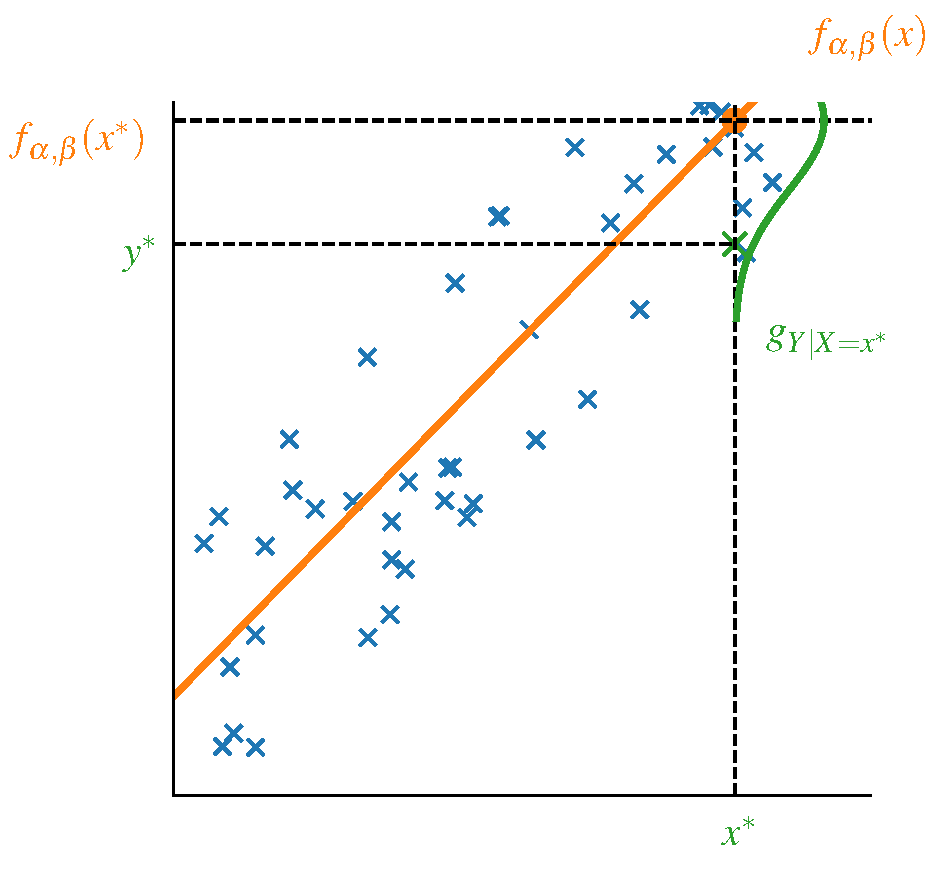
\includegraphics[width=0.6\textwidth]{figures/erm/linreg}
  \caption{Pour une observation $x^*$ donnée (ici en une dimension), la
    distribution des valeurs possibles de son étiquette est une gaussienne
    centrée en $f(x^*)$. La vraie valeur de l'étiquette est $y^*$.}
  \label{fig:linreg}
\end{figure}


\subsection{Estimation par maximum de vraisemblance $\bullet$}
\label{sec:least_squares}
Sous l'hypothèse~\eqref{eq:param_bayes}, nous pouvons estimer $\bbeta$ en
maximisant la log-vraisemblance de l'échantillon
$\left((\xx^1, y^1), (\xx^2, y^2), \dots, (\xx^n, y^n) \right), $ qui est la
réalisation d'un échantillon aléatoire constitué de $n$ copies i.i.d. de
$(X, Y)$.  En notant $g_{X,Y}$ la densité jointe de $(X, Y)$; $g_{Y|X=x}$ la
densité de $Y|X=x$; et $g_X$ la densité de $X$, cette log-vraisemblance s'écrit
\begin{equation*}
  \ell\left((\xx^1, y^1), (\xx^2, y^2), \dots, (\xx^n, y^n); \bbeta  \right)
  = \ln \prod_{i=1}^n g_{X, Y}(\xx^i, y^i) 
  = \ln \prod_{i=1}^n g_{Y|X=\xx^i}(y^i) + \ln \prod_{i=1}^n
  g_X(\xx^i)
\end{equation*}
et donc    
\begin{equation*}
  \ell\left((\xx^1, y^1), (\xx^2, y^2), \dots, (\xx^n, y^n); \bbeta  \right)
  = - \frac1{2\sigma^2} \sum_{i=1}^n \left(y^i -
    f_{\bbeta}(\xx^i) \right)^2 + \Ccal,
\end{equation*}
avec $\Ccal$ une constante par rapport à $\bbeta$, qui provient d'une part du
coefficient $\frac1{\sqrt{2\pi}}$ de la distribution normale et d'autre part
des $g_X(\xx^i)$.

Ainsi, maximiser la vraisemblance dans ce contexte de bruit gaussien centré
revient à minimiser 
\[\sum_{i=1}^n \left(y^i - f_{\bbeta}(\xx^i) \right)^2.\]
On retrouve ici la méthode des moindres carrés de l'équation~\eqref{eq:erm_parametric}.

\section{Régression linéaire}
\label{sec:linreg}
Nous allons maintenant appliquer la minimisation des moindres carrés au cas où
$\FF$ est l'ensemble des fonctions linéaires de $p$ variables.

\subsection{Formulation}
Nous choisissons une fonction de décision $f$ de la forme
\begin{equation}
  \label{eq:linear_decision}
  f: \xx \mapsto \beta_0 + \sum_{j=1}^p \beta_j x_j.
\end{equation}
Ici, $\bbeta \in \RR^{p+1}$ et donc $m=p+1$.

\subsection{Solution}
On appelle \textbf{régression linéaire} le modèle de la forme
$f: \xx \mapsto \beta_0 + \sum_{j=1}^p \beta_j x_j$ dont les coefficients sont
obtenus par minimisation de la somme des moindres carrés, à savoir :
\begin{equation}
  \label{eq:linreg}
  \argmin_{\bbeta \in \RR^{p+1}}  \sum_{i=1}^n \left(y^i - \left(\beta_0 + 
      \sum_{j=1}^p \beta_j x^i_j \right)\right)^2.
\end{equation}
  
Nous pouvons réécrire le problème~\ref{eq:linreg} sous forme matricielle, en
ajoutant à gauche à la matrice d'observations $X \in \RR^p$ une colonne de 1 :
\begin{equation}
  \label{eq:added_ones}
  X \leftarrow   \begin{pmatrix}
    1 & x_1^1 & \cdots & x_p^1 \\
    \vdots & \vdots & \cdots & \vdots \\
    1 & x_1^n& \cdots & x_p^n \\
  \end{pmatrix}.
\end{equation}

La somme des moindres carrés s'écrit alors
\begin{equation}
  \label{eq:rss_linreg}
  \text{RSS} = \left(\yy - X \bbeta\right)^\top \left(\yy -  X \bbeta\right).
\end{equation}

Il s'agit d'une forme quadratique convexe en $\bbeta$, que l'on peut donc
minimiser en annulant son gradient
$\nabla_{\bbeta} \text{RSS} = -2 X^\top \left(\yy - X \bbeta \right)$. La somme
des moindres carrés est minimale si $\bbeta$ vérifie 
\begin{equation}
  \label{eq:linreg_sol}
  X^\top X \bbeta = X^\top \yy.
\end{equation}
  
\paragraph{Solution explicite}
Si le rang de la matrice $X$ est égal à son nombre de colonnes, alors
$X^\top X$ est inversible et la somme des moindres carrés de
l'équation~\eqref{eq:rss_linreg} est minimisée pour
\begin{equation*}
  \bbeta^* = \left(X^\top X \right)^{-1} X^\top \yy.
\end{equation*}

Si $X^\top X$ n'est pas inversible, on pourra néanmoins trouver une solution
(non unique) pour $\bbeta$ en utilisant à la place de
$\left(X^\top X \right)^{-1}$ un pseudo-inverse (par exemple, celui de
Moore-Penrose) de $X^\top X$, c'est-à-dire une matrice $M$ telle que
$X^\top X M X^\top X = X^\top X.$

\paragraph{Méthode de descente}
On peut aussi (et ce sera préférable quand $p$ est grand et que l'inversion de
la matrice $X^\top X \in \RR^{p \times p}$ est donc coûteuse) obtenir une
estimation de $\bbeta$ par un algorithme à directions de descente.

\paragraph{Interprétation} La régression linéaire produit un modèle interprétable, au sens où les
$\beta_j$ permettent de comprendre l'importance relative des variables sur la
prédiction. En effet, plus $\lvert \beta_j \rvert$ est grande, plus la $j$-ème
variable a un effet important sur la prédiction, et le signe de $\beta_j$ nous
indique la direction de cet effet.

Attention ! Cette interprétation n'est valide que si les variables ne sont pas
corrélées, et que $x_j$ peut être modifiée sans perturber les autres
variables. De plus, si les variables sont corrélées, $X$ n'est pas de rang
colonne plein et $X^\top X$ n'est donc pas inversible. Ainsi la régression
linéaire admet plusieurs solutions. Intuitivement, on peut passer de l'une à
l'autre de ces solutions car une perturbation d'un des poids $\beta_j$ peut
être compensée en modifiant les poids des variables corrélées à $x_j$.

\paragraph{Remarque} % Nous avons traité ici de problèmes de \textit{régression}
% uniquement.
Nous traiterons de classification paramétrique dans la PC~5.


%-*- coding: utf-8 -*-
\section{QCM}
\paragraph{Question 1.} Quand le nombre d'observations tend vers l'infini, 
\begin{itemize}
\item[$\square$] le risque empirique d'un modèle converge vers le risque de ce modèle ; 
\item[$\square$] le risque empirique minimal converge vers le risque minimal ; 
\item[$\square$] le minimiseur du risque empirique converge vers le minimiseur du risque.
\end{itemize}

\paragraph{Question 2.} Supposons un problème de classification en 2
dimensions, avec $n$ observations. Nous considérons comme espace des hypothèses
l'ensemble des unions de $K$ cercles ($K > 0$ est fixé) : les points intérieurs
à ces cercles sont étiquetés positifs, les autres négatifs. Alors
\begin{itemize}
\item[$\square$] Il ne s'agit pas d'un modèle paramétrique.
\item[$\square$] Il s'agit d'un modèle paramétrique à $K$ paramètres.
\item[$\square$] Il s'agit d'un modèle paramétrique à $2K$ paramètres.
\item[$\square$] Il s'agit d'un modèle paramétrique à $3K$ paramètres.
\end{itemize}

\paragraph{Question 3.} Quel algorithme préférer pour entraîner une régression
linéaire sur un jeu de données contenant $n$ observations et $p$ variables :
\begin{itemize}
\item Si $n=10^5$ et $p=5$ ?
  \begin{itemize}
  \item[$\square$] Une inversion de matrice.
  \item[$\square$] Un algorithme du gradient.
  \end{itemize}
\item Si $n=10^5$ et $p=10^5$ ?
  \begin{itemize}
  \item[$\square$] Une inversion de matrice.
  \item[$\square$] Un algorithme du gradient.
  \end{itemize}
\end{itemize}

\section*{Solution}
{%
\noindent
\rotatebox[origin=c]{180}{%
\noindent
\begin{minipage}[t]{\linewidth}
\paragraph{Question 1.} Seule la première proposition est vraie. \newline

\paragraph{Question 2.} Il s'agit d'un modèle paramétrique et nous avons besoin
de $3K$ paramètres pour déterminer les coordonnées de $K$ cercles (coordonnées
du centre + rayon). \newline

\paragraph{Question 3.}  Lorsque la matrice $X^\top X$ (de dimensions
$p \times p$) est de petite taille (peu de variables), on pourra utiliser un
algorithme d'inversion de matrice. Sinon, un algorithme du gradient sera plus
approprié.
\end{minipage}%
}%

%%% Local Variables:
%%% mode: latex
%%% TeX-master: "../../sdd_2025_poly"
%%% End:



%%% Local Variables:
%%% mode: latex
%%% TeX-master: "../sdd_2025_poly"
%%% End:
\clearpage 

\chapter{Généralisation}
%-*- coding: utf-8 -*-    
\label{chap:generalisation}

\paragraph{Notions :} généralisation ; surapprentissage ; sélection de modèle
; validation croisée ; régularisation des modèles paramétriques linéaires
\paragraph{Objectifs pédagogiques :} 
\begin{itemize}      
  \setlength{\itemsep}{3pt}
\item Détecter un risque de surapprentissage ;
\item Mettre en place un cadre permettant de sélectionner un modèle parmi
  plusieurs et d'estimer sa performance en généralisation ;
\item Utiliser la régularisation pour éviter le surapprentissage ;
\item Manipuler les régularisations $\ell_1$ et $\ell_2$ sur des modèles linéaires.
\end{itemize}

\section{Généralisation et surapprentissage}
\subsection{Généralisation}
Imaginons un algorithme qui, pour prédire l'étiquette d'une observation $\xx$,
retourne son étiquette si $\xx$ appartient aux données dont l'étiquette est
connue, et une valeur aléatoire sinon. Ce modèle, qui en quelque sorte «
apprend par c\oe{}ur », aura un risque empirique nul (et donc minimal) quelle
que soit la fonction de coût choisie. Cependant, il fera de très mauvaises
prédictions pour toute nouvelle observation.

\begin{encadre} {Évaluer un modèle de machine learning sur
    les données sur lesquelles il a été appris ne nous permet absolument pas de
    savoir comment il se comportera sur de nouvelles données, en d'autres mots,
    sa capacité à \textbf{généraliser}. C'est un des aspects les plus
    importants de l'apprentissage automatique.}
\end{encadre}

\subsection{Surapprentissage}
L'exemple, certes extrême, que nous avons pris plus haut, illustre que l'on
peut facilement mettre au point une procédure d'apprentissage qui produise un
modèle qui fait de bonnes prédictions sur les données utilisées pour le
construire, mais généralise mal. Au lieu de modéliser la vraie nature des
objets qui nous intéressent ($\Phi(X)$ dans
l'équation~\eqref{eq:probabilistic_ml}), un tel modèle capture aussi (voire
surtout) un bruit ($\epsilon$ dans l'équation~\eqref{eq:probabilistic_ml}) qui
n'est pas pertinent pour l'application considérée.

On dit d'un modèle qui, plutôt que de capturer la nature des objets à
étiqueter, modélise aussi le bruit et ne sera pas en mesure de généraliser
qu'il \textbf{surapprend} (\textit{overfits} en anglais). 
Un modèle qui surapprend est généralement un modèle \textbf{trop complexe}, qui
\og colle \fg~trop aux données et capture donc aussi leur bruit.
  
À l'inverse, il est aussi possible de construire un modèle \textbf{trop simple},
dont les performances ne soient bonnes ni sur les données utilisées pour le
construire, ni en généralisation. 
On dit d'un modèle qui est trop simple pour avoir de bonnes performances même
sur les données utilisées pour le construire qu'il \textbf{sous-apprend} (\textit{underfits} en
anglais).

Ces concepts sont illustrés sur la figure~\ref{fig:overfit_class} pour un
problème de classification binaire et la figure~\ref{fig:overfit_regr} pour un
problème de régression.

\begin{figure}[h]
  \begin{subfigure}[t]{0.48\textwidth}
    \centering
    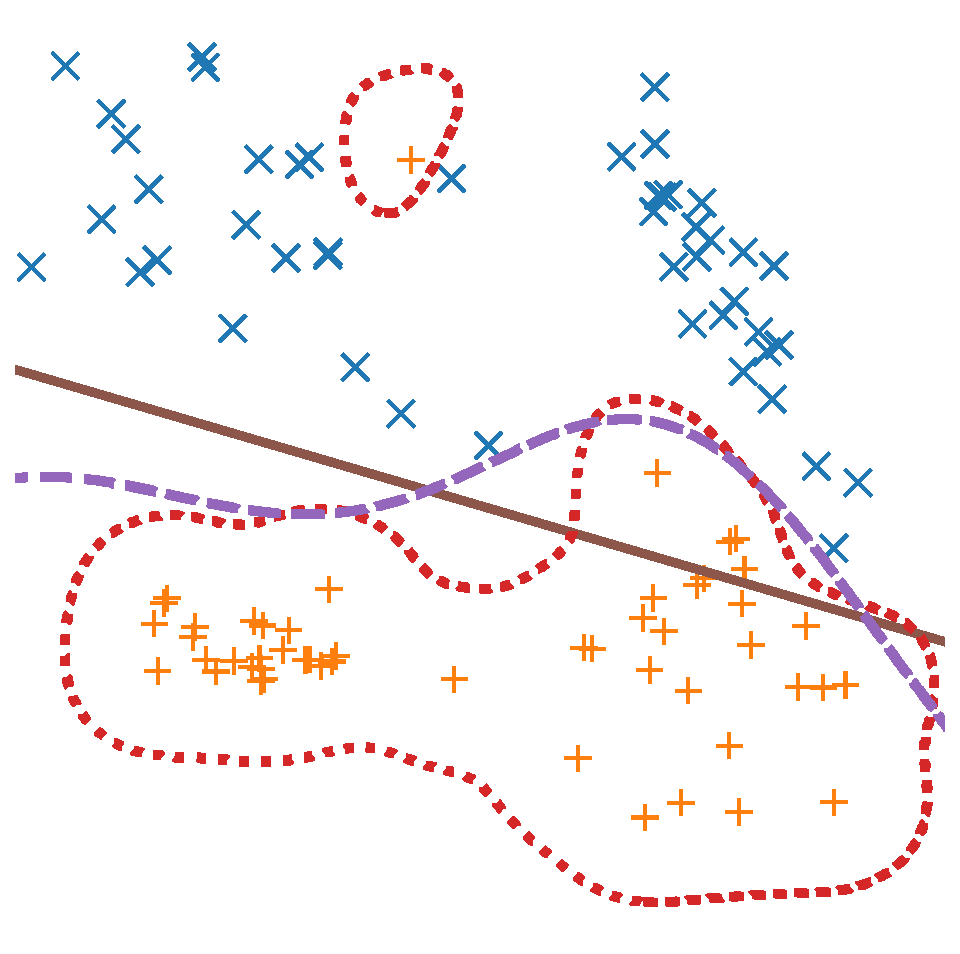
\includegraphics[width=\textwidth]{figures/generalisation/overfit_class}
    \caption{Pour séparer les observations négatives (x) des observations
      positives (+), la droite en trait plein sous-apprend. La frontière de
      séparation en pointillés ne fait aucune erreur sur les données mais est
      susceptible de surapprendre. La frontière de séparation en trait
      discontinu est un bon compromis.}
    \label{fig:overfit_class}
  \end{subfigure}
  \hfill
  \begin{subfigure}[t]{0.48\textwidth}
    \centering
    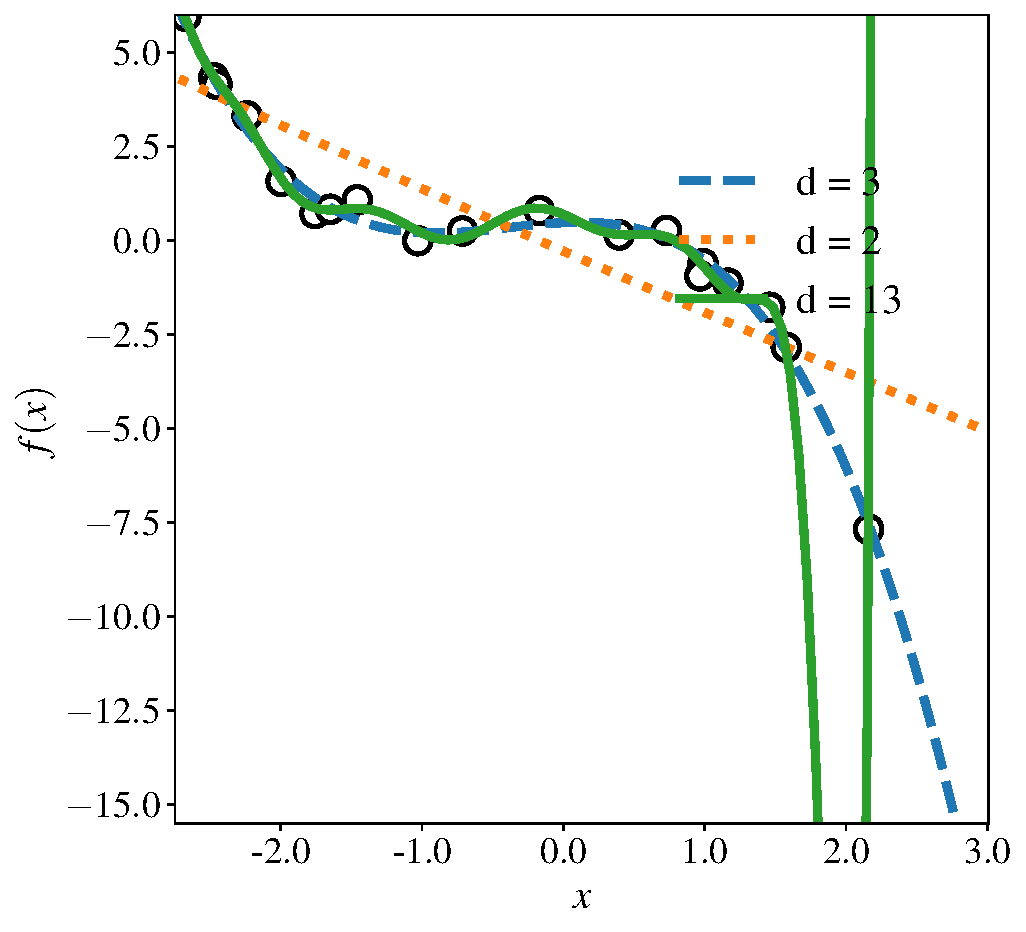
\includegraphics[width=\textwidth]{figures/generalisation/overfit_regr}
    \caption{Les étiquettes $y$ des observations (représentées par des points)
      ont été générées à partir d'un polynôme de degré $d=3$. Le modèle de
      degré $d=2$ approxime très mal les données et sous-apprend, tandis que
      celui de degré $d=13$, dont le risque empirique est plus faible,
      surapprend.}
    \label{fig:overfit_regr}
  \end{subfigure}
  \caption{Sous-apprentissage et surapprentissage}
\end{figure}

\subsection{Compromis biais-variance $\bullet$}
\label{sec:bias_variance}
Supposons disposer d'un jeu de données $\DD = \{\xx^i, y^i\}_{i=1, \dots, n}$
de $n$ observations en $p$ dimensions et leurs étiquettes réelles. Nous
supposons comme au chapitre précédent que les couples $(\xx^i, y^i)$ sont les
réalisations de $n$ vecteurs aléatoires de même loi qu'un couple de variables
aléatoire $(X, Y)$, $X$ étant un vecteur aléatoire $p$-dimensionnel et $Y$ une
variable aléatoire réelle à valeurs dans $\YY$, et qu'il existe une fonction
$\Phi \colon \RR^p \to \YY$ et une variable aléatoire réelle $\epsilon$
telle que
  \begin{equation}
  Y = \Phi(X) + \epsilon.
\end{equation}
Nous supposons de plus que $\epsilon$ est d'espérance nulle et de variance
$\sigma^2$.

Fixons maintenant un couple $(\xx, y) \in \RR^p \times \YY$. Nous pouvons
considérer que la prédiction $f(\xx)$ d'un modèle $f$ appris sur $\DD$ est une
estimation de $\Phi(\xx)$, autrement dit la réalisation d'une variable aléatoire
$F_n$ qui est une fonction d'un échantillon aléatoire de $n$ copies iid de
$(X, Y)$. Nous pouvons alors calculer l'erreur quadratique moyenne de la
prédiction $F_n$ :
\begin{align*}
  & \EE\left((y-F_n)^2\right)  = \EE\left((\Phi(\xx) + \epsilon - F_n)^2   \right)
   = \EE\left((\Phi(\xx) - \EE(F_n) + \EE(F_n) - F_n  + \epsilon )^2   \right) \\
  & = \EE\left((\Phi(\xx) - \EE(F_n))^2 + (\EE(F_n) - F_n  + \epsilon )^2 + 2
    (\Phi(\xx) - \EE(F_n))(\EE(F_n) - F_n  + \epsilon) \right) \\
  & = (\Phi(\xx) - \EE(F_n))^2 + \EE\left((F_n - \EE(F_n) - \epsilon )^2  \right) + 2
    (\Phi(\xx) - \EE(F_n))  \EE\left( \EE(F_n) - F_n  + \epsilon \right) \\
  & =  \text{B}(F_n)^2  + 
    \EE \left((F_n - \EE(F_n))^2 + \epsilon^2 - 2 \epsilon (F_n - \EE(F_n)) \right) + 2
    (\Phi(\xx) - \EE(F_n))  \left( \EE(F_n) - \EE(F_n)  + \EE(\epsilon) \right) \\
  & =  \text{B}(F_n)^2  + 
    \EE \left((F_n - \EE(F_n))^2 \right) + \EE(\epsilon^2) - 2 \EE\left(\epsilon (F_n - \EE(F_n)) \right) \\
    & = \text{B}(F_n)^2 + \VV(F_n) + \sigma^2.
\end{align*}
Le passage de la deuxième à la troisième ligne se fait par linéarité de
l'espérance et en observant que $\Phi(\xx)$ et $\EE(F_n)$ sont déterministes
(ce sont des nombres, pas des variables aléatoires).

Le troisième terme de la somme de la quatrième ligne disparait à la cinquième
car $\EE(\epsilon)=0$.

Enfin, le passage à la dernière ligne se fait en supposant que $\epsilon$ et
$F_n$ sont indépendants ; on a alors
$\EE\left(\epsilon (F_n - \EE(F_n)) \right) = \EE(\epsilon) \EE(F_n -
\EE(F_n)).$ De plus, $\EE(\epsilon^2) = \VV(\epsilon)$ car $\EE(\epsilon)=0$.

Ainsi, l'erreur quadratique moyenne est la somme
\begin{itemize}
\item du carré du biais de l'estimateur, qui quantifie à quel point les étiquettes prédites diffèrent des vraies étiquettes ;
\item de la variance de l'estimateur, qui quantifie à quel point les étiquettes
  prédites pour le même individu $\xx$ diffèrent selon les données d'entrée
  (i.e. les réalisations des n copies iid de $(X, Y)$) ;
\item de la variance du bruit, aussi appelée \textbf{erreur irréductible} : ce terme sera là même si l'estimation de $\Phi$ est exacte.
\end{itemize}

On retrouve ici le compromis biais-variance (cf
section~\ref{sec:precision_estimateur}) : un modèle biaisé peut, s'il a une variance plus faible, faire de meilleures prédictions qu'un modèle non-biaisé.



%Pour mieux comprendre le risque d'un modèle $f: \XX \rightarrow \YY$, nous
% pouvons le comparer à l'erreur minimale $\Rcal^*$ qui peut être atteinte par
% n'importe quelle fonction mesurable de $\XX$ dans $\YY$ : c'est ce qu'on
% appelle l'\textit{excès d'erreur}, et que l'on peut décomposer de la façon
% suivante :
% \begin{equation}
%   \label{eq:estimation_approximation}
%   \Rcal(f) - \Rcal^* = \left[ \Rcal(f) - \min_{h \in \FF} 
%     \Rcal(h) \right]
%   + \left[ \min_{h \in \FF} \Rcal(h) - \Rcal^* \right]
% \end{equation}

% Le premier terme, $\Rcal(f) - \min_{h \in \FF} \Rcal(h)$, quantifie la distance
% entre le modèle $f$ et le modèle optimal sur $\FF$. C'est ce que l'on appelle
% {\it l'erreur d'estimation.}

% Le second terme, $\min_{h \in \FF} \Rcal(h) - \Rcal^*$, quantifie la qualité du
% modèle optimal sur $\FF$, autrement dit, la qualité du choix de l'espace des
% hypothèses. C'est ce que l'on appelle {\it l'erreur d'approximation.} Si $\FF$
% est l'ensemble des fonctions mesurables, alors l'erreur d'approximation est
% nulle.

% Ainsi, l'écriture~\ref{eq:estimation_approximation} permet de décomposer
% l'erreur entre un terme qui découle de la qualité de l'espace des hypothèses et
% un autre qui découle de la qualité de la procédure d'optimisation utilisée. En
% pratique, sauf dans des cas très particuliers où cela est rendu possible par
% construction, il n'est pas possible de calculer ces termes d'erreur.
% Cependant, cette écriture nous permet de comprendre le problème suivant :
% choisir un espace des hypothèses plus large permet généralement de réduire
% l'erreur d'approximation, car un modèle plus proche de la réalité a plus de
% chances de se trouver dans cet espace. Cependant, puisque cet espace est plus
% vaste, la solution optimale y est aussi généralement plus difficile à trouver :
% l'erreur d'estimation, elle, augmente. C'est dans ce cas qu'il y a
% surapprentissage. \\

% Un espace des hypothèses plus large permet généralement de construire des
% modèles plus complexes : par exemple, l'ensemble des droites vs. l'ensemble des
% polynômes de degré 13 (cf. figure~\ref{fig:overfit_regr}). C'est une variante du
% principe du \textbf{rasoir d'Ockham}, selon lequel les
% hypothèses les plus simples sont les plus vraisemblables.

% Il y a donc un compromis entre erreur d'approximation et erreur d'estimation :
% il est difficile de réduire l'une sans augmenter l'autre. Ce compromis est
% généralement appelé \textbf{compromis biais-variance} : l'erreur d'approximation
% correspond au \textbf{biais} de la procédure d'apprentissage, tandis que l'erreur
% d'estimation correspond à sa \textbf{variance}. % On retrouvera ce compromis dans
% % l'estimation bayésienne de paramètres à la
% % section~\ref{sec:bias_variance_bayes}.

% Considérons par exemple pour un problème de régression un espace des hypothèses
% naïf qui ne contient que des fonctions constantes. Supposons que les étiquettes
% soient générées par une distribution normale centrée en $a$. Quelles que soient
% les données observées, la procédure d'apprentissage va construire un modèle qui
% retourne $a$ quelle que soit l'observation concernée : la \textbf{variance} de la
% procédure par rapport au jeu de données est très faible. À l'inverse, comme la
% fonction de prédiction apprise est très peu sensible au jeu de données, il y a
% un \textbf{biais} très important qui conduit à construire des prédicteurs qui
% retournent $a$ pour toutes les observations.

\section{Sélection de modèle}
Le théorème du \textit{no free lunch} % de~\citet{wolpert1997}
indique qu'aucun
algorithme de machine learning ne peut bien fonctionner pour \textbf{tous} les
problèmes d'apprentissage : un algorithme qui fonctionne bien sur un type
particulier de problèmes le compensera en fonctionnant moins bien sur d'autres
types de problèmes. En d'autres termes, il n'y a pas de \og baguette magique
\fg~qui puisse résoudre tous nos problèmes de machine learning, et il est donc
essentiel, pour un problème donné, de tester plusieurs possibilités afin de
sélectionner le modèle optimal. Notons au passage que plusieurs critères
peuvent intervenir dans ce choix : non seulement celui de la qualité des
prédictions, qui nous intéresse dans ce chapitre, mais aussi celui des
ressources de calcul nécessaires, qui peuvent être un facteur limitant en
pratique.

L'erreur empirique mesurée sur les observations qui ont permis de construire le
modèle est un mauvais estimateur de l'erreur du modèle sur l'ensemble des
données possibles, ou \textbf{erreur de généralisation} : si le modèle
surapprend, cette erreur empirique peut être proche de zéro voire nulle,
tandis que l'erreur de généralisation peut être arbitrairement grande.

\subsection{Jeu de test}
Il est donc indispensable d'utiliser pour évaluer un modèle des données
étiquetées qui n'ont pas servi à le construire. La manière la plus simple d'y
parvenir est de mettre de côté une partie des observations, réservées à
l'évaluation du modèle, et d'utiliser uniquement le reste des données pour le
construire.

Étant donné un jeu de données $\DD = \{(\xx^i, y^i)\}_{i=1, \dots, n}$,
partitionné en deux jeux $\DD_{\text{tr}}$ et $\DD_{\text{te}}$, on appelle
\textbf{jeu d'entraînement} (\textit{training set} en anglais) l'ensemble
$\DD_{\text{tr}}$ utilisé pour entraîner un modèle prédictif, et \textbf{jeu de
  test} (\textit{test set} en anglais) l'ensemble $\DD_{\text{te}}$ utilisé pour
son évaluation.

Comme nous n'avons pas utilisé le jeu de test pour entraîner notre modèle, il
peut être considéré comme un jeu de données \og nouvelles \fg. La perte
calculée sur ce jeu de test est un estimateur de l'erreur de généralisation.

Cela correspond à ce que nous avons fait dans la PC~3 et au début du Projet numérique.

\subsection{Jeu de validation}
Considérons maintenant la situation dans laquelle nous voulons choisir entre
$K$ modèles, appris chacun par un algorithme différent. Notons qu'il peut
s'agir ici d'utiliser des algorithmes d'apprentissage différents (plus proches
voisins, régression linéaire, réseau de neurones), ou d'un même algorithme
d'apprentissage avec plusieurs valeurs d'un ou plusieurs
\textbf{hyperparamètres}. Un hyperparamètre est un paramètre de l'algorithme
d'apprentissage (et non pas du modèle) ; il peut s'agir par exemple du nombre
de voisins $k$ considérés dans un algorithme des plus proches voisins (cf Projet numérique), du
coefficient de régularisation $\lambda$ dans un lasso (cf
section~\ref{sec:lasso}), ou du nombre de neurones dans une couche cachée d'un
perceptron multi-couche (cf section~\ref{sec:mlp}).

Nous pouvons alors entraîner chacun des modèles sur le jeu de
données d'entraînement, obtenant ainsi $K$ fonctions de décision
$f_1, f_2, \dots, f_K$, puis calculer l'erreur de chacun de ces modèles sur le
jeu de test. Nous pouvons ensuite choisir comme modèle celui qui a la plus
petite erreur sur le jeu de test:
\begin{equation}
  \hat f = \argmin_{k=1, \dots, K} \frac{1}{|\DD_{\text{te}}|} 
  \sum_{(\xx, y) \in \DD_{\text{te}}} L(y, f_k(\xx)).
\end{equation}
Mais quelle est son erreur de généralisation ? Comme nous avons utilisé
$\DD_{\text{te}}$ pour sélectionner le modèle, il ne représente plus un
jeu indépendant composé de données nouvelles, inutilisées pour déterminer le
modèle.

La solution est alors de découper notre jeu de données en \textbf{trois} parties~:
\begin{itemize}
\item Un \textbf{jeu d'entraînement}
  $\DD_{\text{tr}}$ sur lequel nous pourrons entraîner nos $K$ algorithmes
  d'apprentissage ;
\item Un \textbf{jeu de validation} ({\it validation set} en anglais)
  $\DD_{\text{val}}$ sur lequel nous évaluerons les $K$ modèles ainsi
  obtenus, afin de \textbf{sélectionner} un modèle définitif ;
\item Un \textbf{jeu de test} $\DD_{\text{te}}$ sur lequel nous évaluerons enfin
  l'erreur de généralisation du modèle choisi.
\end{itemize}

On voit ici qu'il est important de distinguer la {\it sélection} d'un modèle de
son \textbf{évaluation} : les faire sur les mêmes données peut nous conduire à
sous-estimer l'erreur de généralisation et le surapprentissage du modèle
choisi.

Une fois un modèle sélectionné, on peut le ré-entraîner sur l'union du jeu
d'entraînement et du jeu de validation afin de construire un modèle final.

\subsection{Validation croisée}
\label{sec:crossval}
La séparation d'un jeu de données en un jeu d'entraînement et un jeu de test
est nécessairement arbitraire. Nous risquons ainsi d'avoir, par hasard, créé
des jeux de données qui ne sont pas représentatifs. Pour éviter cet écueil, il
est souhaitable de reproduire plusieurs fois la procédure, puis de moyenner les
résultats obtenus afin de moyenner ces effets aléatoires. Le cadre le plus
classique pour ce faire est celui de la \textbf{validation croisée}, illustré sur
la figure~\ref{fig:crossval}

\begin{figure}[h]
  \centering
  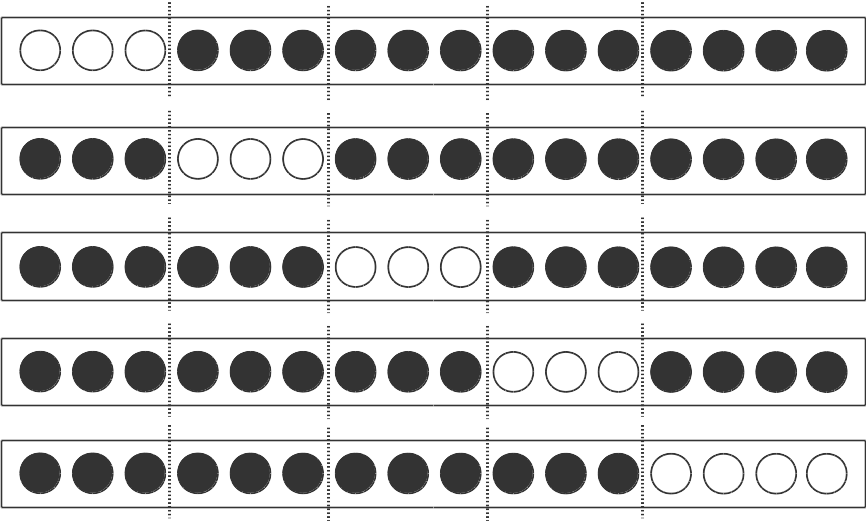
\includegraphics[width=0.5\textwidth]{figures/generalisation/crossval}
  \caption{Une validation croisée en 5 {\it folds} : Chaque observation
    appartient à un des 5 jeux de validation (en blanc) et aux 4 autres jeux
    d'entraînement (en noir).}
  \label{fig:crossval}
\end{figure}

Étant donné un jeu $\DD$ de $n$ observations, et un nombre $K$ (généralement
choisi égal à 5 ou 10), on appelle {\it validation croisée} la procédure qui
consiste à
\begin{enumerate}
\item partitionner $\DD$ en $K$ parties de tailles sensiblement similaires,
  $\DD_1, \DD_2, \dots, \DD_K$
\item pour chaque valeur de $k=1, \dots, K$,
  \begin{itemize}
  \item entraîner un modèle sur $\bigcup_{l \neq k} \DD_l$
  \item évaluer ce modèle sur $\DD_k$.
  \end{itemize}
\end{enumerate}
Chaque partition de $\DD$ en deux ensembles $\DD_k$ et $\bigcup_{l \neq
  k} \DD_l$ est appelée un \textbf{fold} de la validation croisée.

Chaque observation étiquetée du jeu $\DD$ appartient à un unique jeu de test,
et à $(K-1)$ jeux d'entraînement. Ainsi, cette procédure génère une prédiction
par observation de $\DD$. Pour conclure sur la performance du modèle, on évalue
chacun des $K$ prédicteurs sur le jeu de test $\DD_k$ correspondant, et on
moyenne ces performances. Cette approche permet aussi de rapporter l'écart-type
de ces performances, ce qui permet de se faire une meilleure idée de la
variabilité de la qualité des prédictions en fonction des données
d'entraînement.

\section{Critères de performance}
\subsection{Matrice de confusion et critères dérivés}
\label{sec:confusion_matrix}
Comme nous l'avons vu, le nombre d'erreurs de classification permet d'évaluer
la qualité d'un modèle prédictif. Notons que l'on préférera généralement
décrire le nombre d'erreurs comme une fraction du nombre d'exemples : un taux
d'erreur de $1\%$ est plus parlant qu'un nombre absolu d'erreurs.
 
Mais toutes les erreurs ne se valent pas nécessairement. Prenons l'exemple d'un
modèle qui prédise si oui ou non une radiographie présente une tumeur
inquiétante : une fausse alerte, qui sera ensuite infirmée par des examens
complémentaires, est moins problématique que de ne pas déceler la tumeur et de
ne pas traiter la personne concernée.  Les performances d'un modèle de
classification binaire peuvent être résumées dans une
\textbf{matrice de confusion} : une matrice $M$ de deux lignes et deux
colonnes, et dont l'entrée $M_{ck}$ est le nombre d'exemples de la classe $c$
pour laquelle l'étiquette $k$ a été prédite.
\begin{table}[h]
	\centering
	\arrayrulecolor{black!70}
	\begin{tabular}[h]{cccc}
		\cmidrule[1.5pt]{3-4}
		& & \multicolumn{2}{c}{\textbf{Classe réelle}} \\ \cmidrule{3-4}
		& & 0 & 1 \\ \midrule[1pt]
		\textbf{Classe}& \multicolumn{1}{|c!{\color{black!70}\vrule width 1pt}}{0} & \cellcolor{gray!20} vrais négatifs (TN) & faux négatifs (FN) \\ 
		\textbf{prédite}& \multicolumn{1}{|c!{\color{black!70}\vrule width 1pt}}{1} & faux positifs (FP) & \cellcolor{gray!20} vrais positifs (TP) \\ 
		\bottomrule[1.5pt]
	\end{tabular}
\end{table}
%\vspace*{-1em}

% On retrouve ici les erreurs de première et de deuxième espèce de la
% section~\ref{sec:test_errors}, qu'on appellera plutôt respectivement faux
% positifs et faux négatifs dans ce contexte.

Il est possible de dériver de nombreux critères d'évaluation construits à
partir de la matrice de confusion, comme la spécificité, la sensibilité, le
rappel ou la F-mesure. Vous pouvez vous référer à la
section~\ref{sec:confusion_matrix_derived} à la fin de ce chapitre, ou à la
\href{https://scikit-learn.org/stable/modules/model_evaluation.html#classification-metrics}{documentation
  de \texttt{sklearn.metrics}}.



\subsection{Courbe ROC $\bullet$}
De nombreux algorithmes de classification ne retournent pas directement une
étiquette de classe, mais utilisent une fonction de décision qui doit ensuite
être seuillée pour devenir une étiquette. Cette fonction de décision peut être
un score arbitraire, ou la probabilité d'appartenir à la classe positive.
  
On appelle \textbf{courbe ROC}, de l'anglais \textbf{Receiver-Operator
  Characteristic} la courbe décrivant l'évolution de la sensibilité en fonction
du complémentaire à 1 de la spécificité, parfois appelé \textbf{antispécificité},
lorsque le seuil de décision change.

Le terme vient des télécommunications, où ces courbes servent à étudier si un
système arrive à séparer le signal du bruit de fond.

On peut synthétiser une courbe ROC par l'aire sous cette courbe, souvent
abrégée \textbf{AUROC} pour \textbf{Area Under the ROC}.

Un exemple de courbe ROC est présenté sur la figure~\ref{fig:roc_curve}. Le
point $(0, 0)$ apparaît quand on utilise comme seuil un nombre supérieur à la
plus grande valeur retournée par la fonction de décision : ainsi, tous les
exemples sont étiquetés négatifs. À l'inverse, le point $(1, 1)$ apparaît quand
on utilise pour seuil une valeur inférieure au plus petit score retourné par la
fonction de décision : tous les exemples sont alors étiquetés positifs.

\begin{figure}[h]
  \centering
  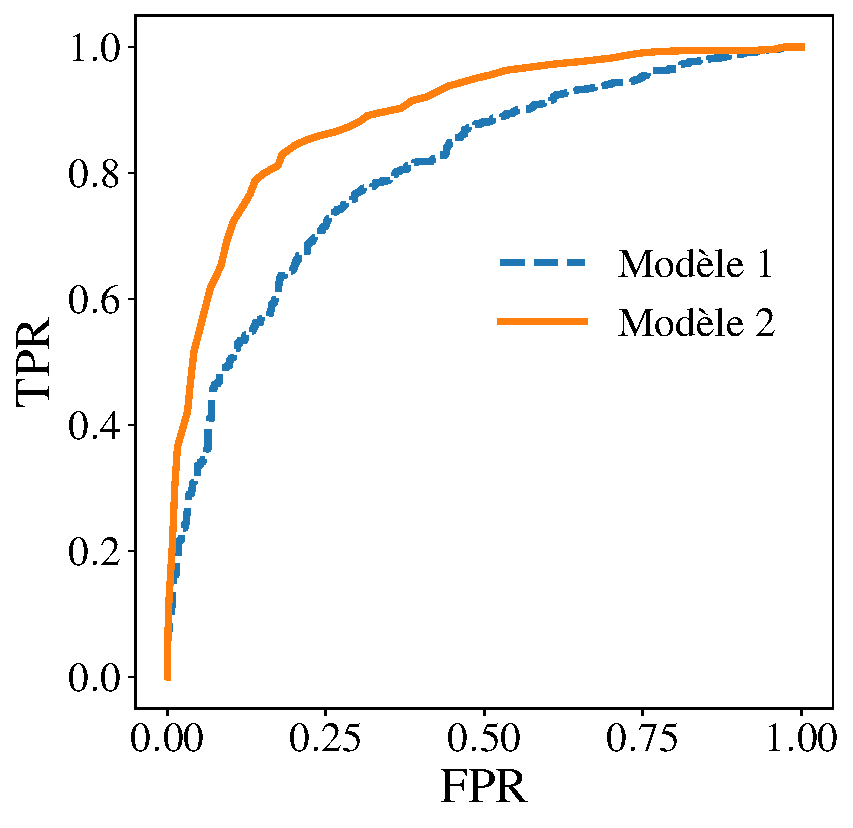
\includegraphics[width=0.5\textwidth]{figures/generalisation/roc_curve}
  \caption{Les courbes ROC de deux modèles.}
  \label{fig:roc_curve}
\end{figure}

Pour construire la courbe ROC, on prend pour seuil les valeurs successives de
la fonction de décision sur notre jeu de données. Ainsi, à chaque nouvelle
valeur de seuil, une observation que l'on prédisait précédemment négative
change d'étiquette. Si cette observation est effectivement positive, la
sensibilité augmente de $1/n_p$ (où $n_p$ est le nombre d'exemples positifs) ;
sinon, c'est l'antispécificité qui augmente de $1/n_n$, où $n_n$ est le nombre
d'exemples négatifs. La courbe ROC est donc une courbe en escaliers.

Un classifieur idéal, qui ne commet aucune erreur, associe systématique des
scores plus faibles aux exemples négatifs qu'aux exemples positifs. Sa courbe
ROC suit donc le coin supérieur gauche du carré $[0, 1]^2$ ; il a une aire sous
la courbe de 1.

La courbe ROC d'un classifieur aléatoire, qui fera sensiblement la même
proportion d'erreurs que de classifications correctes quel que soit le seuil
utilisé, suit la diagonale de ce carré. L'aire sous la courbe ROC d'un
classifieur aléatoire vaut donc 0.5.

On peut enfin utiliser la courbe ROC pour choisir un seuil de décision, à
partir de la sensibilité (ou de la spécificité) que l'on souhaite garantir.

\subsection{Erreurs de régression}
Un premier critère d'évaluation d'un modèle de régression est, nous l'avons vu
à plusieurs reprises, l'\textbf{erreur quadratique moyenne}, ou \textbf{MSE} de
l'anglais \textbf{mean squared error}, à savoir
\begin{equation*}
  \text{MSE} = \frac1n \sum_{i=1}^n \left( f(\xx^i) - y^i \right)^2.
\end{equation*}
Des variantes sont décrites dans la section~\ref{sec:regression_errors} ainsi que dans la \href{https://scikit-learn.org/stable/modules/model_evaluation.html#regression-metrics}{documentation de \texttt{sklearn.metrics}}.

\section{Régularisation}
\label{sec:generalization_regularization}
Le compromis biais-variance nous indique qu'un modèle biaisé peut être plus
précis qu'un modèle non-biaisé. La \textbf{régularisation} consiste ainsi à
ajouter au risque empirique que l'on cherche à minimiser un terme, appelé
\textbf{régulariseur}, qui va biaiser le modèle de sorte à ce que son risque
empirique soit plus élevée, mais son erreur de généralisation plus faible.

Plus un modèle est simple, et moins il a de chances de surapprendre. Pour
limiter le risque de surapprentissage, il est donc souhaitable de limiter la
complexité d'un modèle. Ainsi, le régulariseur peut être vu comme un terme qui
mesure la complexité du modèle. La définition de la complexité d'un modèle est
une notion importante en théorie de l'apprentissage, mais dépasse largement le
cadre de ce cours.

En appelant $\Omega$ le régulariseur, la régularisation consiste donc à
remplacer la minimisation du risque empirique (eq.~\eqref{eq:erm}) par :
\begin{equation}
  \label{eq:regularisation}
  f \in \argmin_{h \in \FF} \frac{1}{n} \sum_{i=1}^n L(y^i, h(\xx^i)) + 
  \lambda \Omega(h),
\end{equation}
où le \textbf{coefficient de régularisation} $\lambda \in \RR_+$ contrôle
l'importance relative de chacun des termes.


Quand $\lambda$ tend vers $+\infty$, le terme de régularisation prend de plus
en plus d'importance, jusqu'à ce qu'il domine le terme d'erreur et que seule
compte la minimisation du régulariseur : il n'y a plus d'apprentissage. % Dans la plupart des cas, le
% régulariseur est minimisé quand $\bbeta = \vec{0}$, et il n'y a plus
% d'apprentissage.
  
À l'inverse, quand $\lambda$ tend vers $0$, le terme de régularisation devient
négligeable devant le terme d'erreur, et la solution de
l'équation~\eqref{eq:regularisation} est un minimiseur du risque
empirique.% $\bbeta$ prendra comme valeur une
% solution de la régression linéaire non régularisée.

Comme tout hyperparamètre, $\lambda$ peut être choisi par validation
croisée. On utilisera généralement une grille de valeurs logarithmique.

La suite de cette section présente des exemples concrets de régularisation
appliquée à la régression linéaire. Nous reprenons les notations de la
section~\ref{sec:linreg}.


\section{Régularisation $\ell_2$  : régression ridge}
\label{sec:ridge_regression}
Une des formes les plus courantes de régularisation % , utilisée dans de
% nombreux domaines faisant intervenir des problèmes inverses mal posés,
consiste à utiliser comme régulariseur la norme $\ell_2$ du vecteur 
$\bbeta$ :  
\begin{equation}
  \label{eq:l2norm_reg}
  \Omega_{\text{ridge}}(\bbeta) = \ltwonorm{\bbeta}^2 = \sum_{j=0}^p \beta_j^2.
\end{equation}


On appelle \textbf{régression ridge} le modèle $f: x \mapsto \bbeta^\top \xx$ dont
les coefficients sont obtenus par
\begin{equation}
  \label{eq:ridgereg}
  \argmin_{\bbeta \in \RR^{p+1}} \ltwonorm{\yy - X \bbeta}^2 + 
  \lambda \; \ltwonorm{\bbeta}^2.
\end{equation}    

\paragraph{Solution}
Le problème~\eqref{eq:ridgereg} est un problème d'optimisation convexe : il s'agit de minimiser une forme
quadratique. Il se résout en annulant le gradient en $\bbeta$ de la fonction
objective :
\begin{equation}
  \nabla_{\bbeta} \left( \ltwonorm{\yy - X \bbeta}^2 + 
    \lambda \ltwonorm{\bbeta}^2 \right) = 0
\end{equation}

En notant $I_p \in \RR^{p \times p}$ la matrice identité en dimension $p,$ on
obtient :
\begin{equation}
  \left( \lambda I_p + X^\top X  \right) \bbeta^* = X^\top \yy.
\end{equation}
Comme $\lambda > 0$, la matrice $\lambda I_p + X^\top X$ est toujours
inversible. Notre problème admet donc toujours une unique solution
explicite. La régularisation par la norme $\ell_2$ a permis de transformer un
problème potentiellement mal posé en un problème bien posé, dont la solution
est :
\begin{equation}
  \label{eq:ridgereg_sol}
  \bbeta^* =  \left( \lambda I_p + X^\top X  \right)^{-1} X^\top \yy.
\end{equation}
  
% Si l'on multiplie la variable $x_j$ par une constante $\alpha$, le coefficient
% correspondant dans la régression linéaire non régularisée est divisé par
% $\alpha.$ En effet, si on appelle $X^*$ la matrice obtenue en remplaçant $x_j$
% par $\alpha x_j$ dans $X$, la solution $\bbeta^*$ de la régression linéaire
% correspondante vérifie $X^* \left( \yy - X^* \bbeta^* \right) = 0$, tandis que
% la solution $\bbeta$ de la régression linéaire sur $X$ vérifie
% $X \left( \yy - X \bbeta \right) = 0.$ Ainsi, changer l'échelle d'une variable
% a comme seul impact sur la régression linéaire non régularisée d'ajuster le
% coefficient correspondant de manière inversement proportionnelle.

% À l'inverse, dans le cas de la régression ridge, remplacer $x_j$ par
% $\alpha x_j$ affecte aussi le terme de régularisation, et a un effet plus
% complexe. L'échelle relative des différentes variables peut donc fortement
% affecter la régression ridge. Il est ainsi recommandé de \textbf{standardiser} les
% variables avant l'apprentissage, c'est-à-dire de toutes les ramener à avoir un
% écart-type de 1 en les divisant par leur écart-type :
% \begin{equation}
%   \label{eq:standardisation}
%   x_j^i \leftarrow \frac{x_j^i}{\sqrt{\frac1n \sum_{i=1}^n \left( x_j^i - 
%         \frac1n \sum_{i=1}^n x_j^i \right)^2}}
% \end{equation}    
% Attention : pour éviter le surapprentissage, il est important que cet
% écart-type soit calculé sur le jeu d'entraînement uniquement, puis appliqué
% ensuite aux jeux de test ou validation.

% La régression ridge a un effet de \og regroupement \fg~sur les variables
% corrélées, au sens où des variables corrélées auront des coefficients
% similaires.

\paragraph{Chemin de régularisation}
On appelle \textbf{chemin de régularisation} l'évolution de la valeur du
coefficient de régression d'une variable en fonction du coefficient de
régularisation $\lambda$.

Le chemin de régularisation permet de comprendre l'effet de la régularisation
sur les valeurs de $\bbeta$. En voici un exemple sur la
figure~\ref{fig:ridge_path}.

\begin{figure}[h]
  \centering
  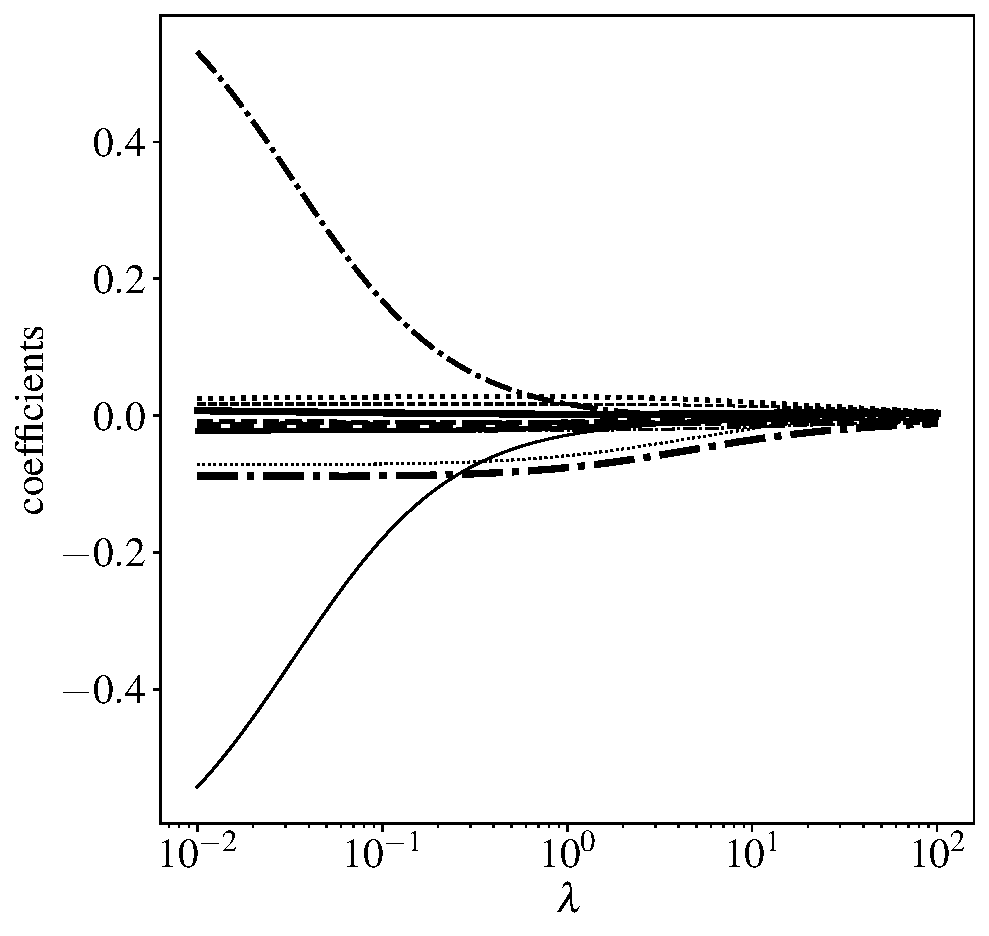
\includegraphics[width=0.5\textwidth]{figures/generalisation/ridge_path}
  \caption{Chemin de régularisation de la régression ridge pour un jeu de
    données avec 12 variables. Chaque ligne représente l'évolution du
    coefficient de régression d'une de ces variables quand $\lambda$ augmente :
    le coefficient évolue de sa valeur dans la régression non régularisée vers
    0.}
  \label{fig:ridge_path}
\end{figure}

\paragraph{Interprétation géométrique}
Étant donnés $\lambda \in \RR_+$, $X \in \RRnp$ et $\yy \in \RR^n$,
il existe un unique $t \in \RR_+$ tel que le problème~\eqref{eq:ridgereg} soit
équivalent à
\begin{equation}
  \label{eq:ridgereg_dual}
  \argmin_{\bbeta \in \RR^{p+1}} \ltwonorm{\yy - X \bbeta}^2 \text{ tel que }
  \ltwonorm{\bbeta}^2 \leq t.
\end{equation}
Preuve : L'équivalence s'obtient par dualité et en écrivant les conditions de
Karun-Kush-Tucker.
  
La régression ridge peut donc être formulée comme un problème d'optimisation
quadratique (minimiser $\ltwonorm{\yy - X \bbeta}^2$) sous contraintes
($\ltwonorm{\bbeta}^2 \leq t$) : la solution doit être contenue dans la boule
$\ell_2$ de rayon $\sqrt{t}$. Sauf dans le cas où l'optimisation sans
contrainte vérifie déjà la condition, cette solution sera sur la frontière de
cette boule, comme illustré sur la figure~\ref{fig:l2reg}.

\begin{figure}[h]
  \centering
  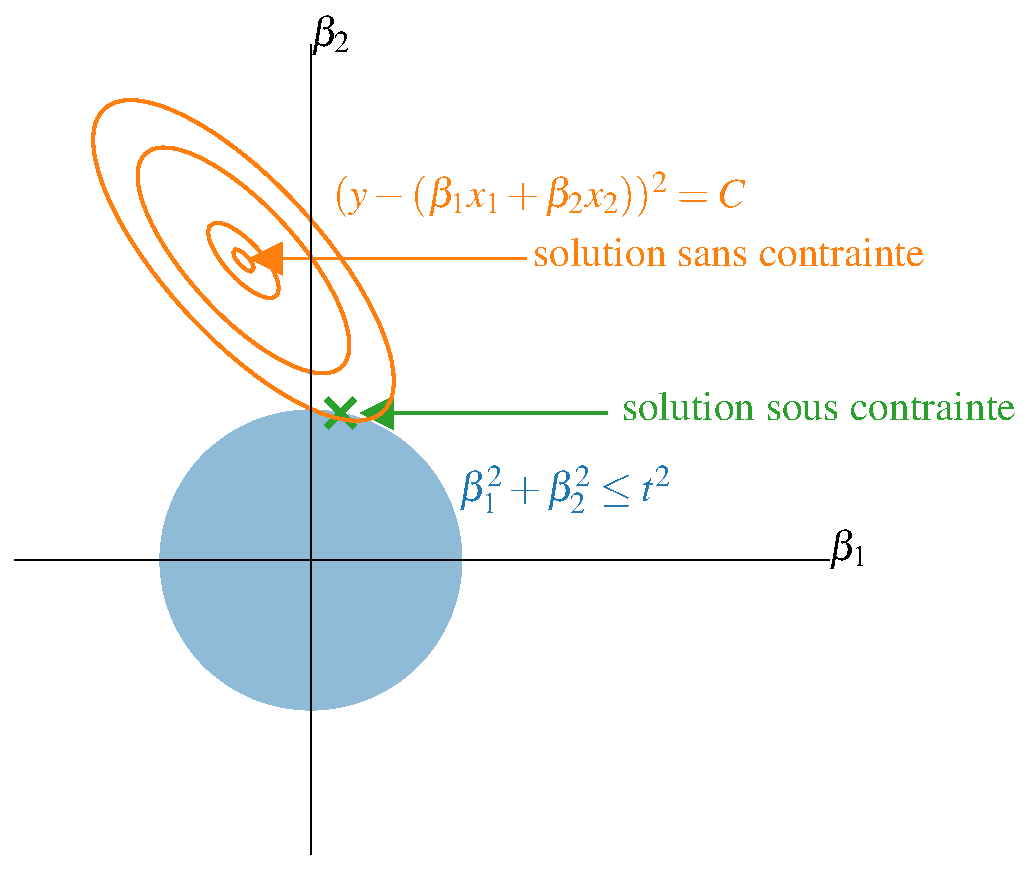
\includegraphics[width=0.55\textwidth]{figures/generalisation/l2reg}
  \caption{La solution du problème d'optimisation sous
    contraintes~\eqref{eq:ridgereg_dual} (ici en deux dimensions) se situe sur
    une ligne de niveau de la somme des moindres carrés tangente à la boule
    $\ell_2$ de rayon $\sqrt{t}$.}
  \label{fig:l2reg}
\end{figure}
  
\section{Régularisation $\ell_1$ : lasso}
\label{sec:lasso}

\paragraph{Parcimonie}
Dans certaines applications, il peut être raisonnable de supposer que
l'étiquette que l'on cherche à prédire n'est expliquée que par un nombre
restreint de variables. Il est dans ce cas souhaitable d'avoir un modèle {\it
  parcimonieux}, ou \textbf{sparse}, c'est-à-dire dans lequel un certain nombre de
coefficients sont nuls : les variables correspondantes peuvent être retirées du
modèle.

Pour ce faire, on peut utiliser comme
régulariseur la norme $\ell_1$ du coefficient $\bbeta$ :
\begin{equation}
  \label{eq:l1norm_reg}
  \Omega_{\text{lasso}}(\bbeta) = \lonenorm{\bbeta} = \sum_{j=0}^p \lvert \beta_j \rvert.
\end{equation}

On appelle \textbf{lasso} le modèle $f: x \mapsto \bbeta^\top \xx$ dont les
coefficients sont obtenus par
\begin{equation}
  \label{eq:lasso}
  \argmin_{\bbeta \in \RR^{p+1}} \ltwonorm{\yy - X \bbeta}^2 + 
  \lambda \lonenorm{\bbeta}.
\end{equation}    
Le nom de lasso est en fait un acronyme, pour \textbf{Least Absolute Shrinkage and
  Selection Operator} : il s'agit d'une méthode qui utilise les valeurs {\it
  absolues} des coefficients (la norme $\ell_1$) pour réduire (\textbf{shrink})
ces coefficients, ce qui permet de \textbf{sélectionner} les variables qui
n'auront pas un coefficient nul. En traitement du signal, le lasso est aussi
connu sous le nom de \textbf{poursuite de base} (\textbf{basis pursuit} en anglais).

En créant un modèle parcimonieux et en permettant d'éliminer les variables
ayant un coefficient nul, le lasso est une méthode de sélection de variables
supervisée. Il s'agit donc aussi d'une méthode de réduction de dimension.

\paragraph{Solution}
Le lasso~\ref{eq:lasso} n'admet pas de solution explicite. On pourra utiliser
un algorithme à directions de descente  pour le résoudre. De plus, il ne s'agit pas
toujours d'un problème strictement convexe (en particulier, quand $p > n$) et
il n'admet donc pas nécessairement une unique solution. En pratique, cela pose
surtout problème quand les variables ne peuvent pas être considérées comme les
réalisations de lois de probabilité continues.
Néanmoins, % s'il est possible que plusieurs $\bbeta$ minimisent la
  % fonction objective du lasso, leur produit à gauche par $X$ vaut toujours la
  % même valeur (par convexité stricte de la fonction de coût) ; cela permet de
  % montrer que 
il est possible de montrer que les coefficients non nuls dans deux solutions
ont nécessairement le même signe. Ainsi, l'effet d'une variable a la même
direction dans toutes les solutions qui la considèrent, ce qui facilite
l'interprétation d'un modèle appris par le lasso.
  
\paragraph{Interprétation géométrique}
Comme précédemment, le problème~\ref{eq:lasso} peut être reformulé comme un
problème d'optimisation quadratique sous contraintes :

Étant donnés $\lambda \in \RR_+$, $X \in \RRnp$ et $\yy \in \RR^n$,
il existe un unique $t \in \RR_+$ tel que le problème~\ref{eq:lasso} soit
équivalent à
\begin{equation}
  \label{eq:lasso_dual}
  \argmin_{\bbeta \in \RR^{p+1}} \ltwonorm{\yy - X \bbeta}^2 \text{ tel que }
  \lonenorm{\bbeta} \leq t.
\end{equation}

La solution doit maintenant être contenue dans la boule $\ell_1$ de rayon
$t$. Comme cette boule a des \og coins \fg, les lignes de niveau de la forme
quadratique sont plus susceptibles d'y être tangentes en un point où une ou
plusieurs coordonnées sont nulles (voir figure~\ref{fig:l1reg}).

\begin{figure}[h]
  \centering 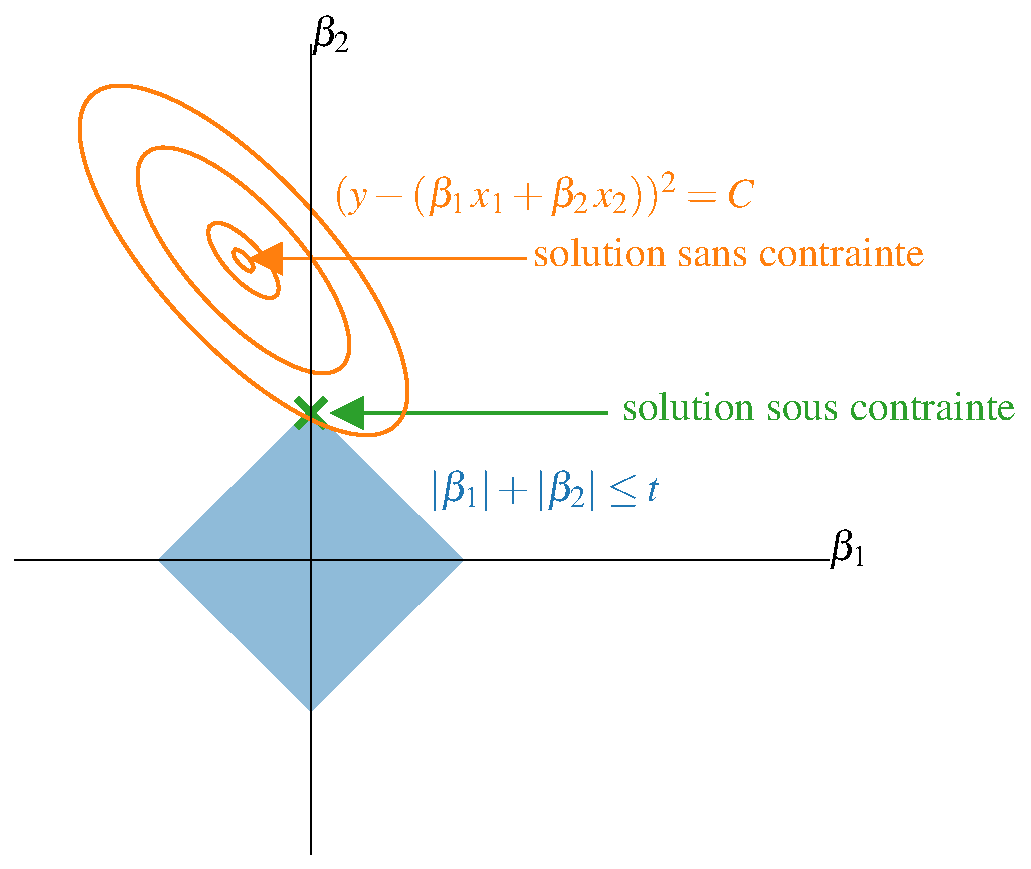
\includegraphics[width=0.55\textwidth]{figures/generalisation/l1reg}
  \caption{La solution du problème d'optimisation sous
    contraintes~\ref{eq:lasso_dual} (ici en deux dimensions) se situe sur
    une ligne de niveau de la somme des moindres carrés tangente à la boule
    $\ell_1$ de rayon $t$.}
  \label{fig:l1reg}
\end{figure}


\paragraph{Chemin de régularisation}
Sur le chemin de régularisation du lasso (par exemple
figure~\ref{fig:lasso_path}, sur les mêmes données que pour la
figure~\ref{fig:ridge_path}), on observe que les variables sortent du modèle
les unes après les autres, jusqu'à ce que tous les coefficients soient nuls. On
remarquera aussi que le chemin de régularisation pour n'importe quelle variable
est linéaire par morceaux ; c'est une propriété du lasso.
\begin{figure}[h]
  \centering
  \includegraphics[width=0.5\textwidth]{figures/generalisation/lasso_path}
  \caption{Chemin de régularisation du lasso pour un jeu de données avec 12
    variables. Chaque ligne représente l'évolution du coefficient de régression
    d'une de ces variables quand $\lambda$ augmente : les variables sont
    éliminées les unes après les autres.}
  \label{fig:lasso_path}
\end{figure}

Si plusieurs variables corrélées contribuent à la prédiction de l'étiquette, le
lasso va avoir tendance à choisir une seule d'entre elles (affectant un poids
de 0 aux autres), plutôt que de répartir les poids équitablement comme la
régression ridge. C'est ainsi qu'on arrive à avoir des modèles très
parcimonieux. Cependant, le choix de cette variable est aléatoire, et peut
changer si l'on répète la procédure d'optimisation. Le lasso a donc tendance à
être instable.

% \section{Exercice : SVM linéaire pour la régression}
% \todo{}

\section{Compléments}
\subsection{Critères d'évaluation d'un modèle de classification binaire dérivés de la matrice de confusion}
\label{sec:confusion_matrix_derived}

On appelle \textbf{vrais positifs} (en anglais \textit{true positives}) les
exemples positifs correctement classifiés ; \textbf{faux positifs} (en anglais
\textit{false positives}) les exemples négatifs étiquetés positifs par le
modèle ; et réciproquement pour les \textbf{vrais négatifs} (\textit{true
  negatives}) et les \textbf{faux négatifs} (\textit{false negatives}). On note
généralement par \textbf{TP} le nombre de vrais positifs, \textbf{FP} le nombre
de faux positifs, \textbf{TN} le nombre de vrais négatifs et \textbf{FN} le
nombre de faux négatifs.

Il est possible de dériver de nombreux critères d'évaluation à partir de la
matrice de confusion. En voici quelques exemples :

On appelle \textbf{rappel} (\textbf{recall} en anglais), ou \textbf{sensibilité} ({\it
  sensitivity} en anglais), le taux de vrais positifs, c'est-à-dire la
proportion d'exemples positifs correctement identifiés comme tels :
\begin{equation*}
  \text{Rappel} = \frac{\text{TP}}{\text{TP} + \text{FN}}.
\end{equation*}

Il est cependant très facile d'avoir un bon rappel en prédisant que \textbf{tous}
les exemples sont positifs. Ainsi, ce critère ne peut pas être utilisé seul. On
lui adjoint ainsi souvent la \textbf{précision} :

On appelle \textbf{précision}, ou \textbf{valeur positive prédictive} (\textbf{positive
  predictive value, PPV}) la proportion de prédictions correctes parmi les
prédictions positives :
\begin{equation*}
  \text{Précision} = \frac{\text{TP}}{\text{TP} + \text{FP}}.
\end{equation*}

De même que l'on peut facilement avoir un très bon rappel au détriment de la
précision, il est aisé d'obtenir une bonne précision (au détriment du rappel)
en faisant très peu de prédictions positives (ce qui réduit le risque qu'elles
soient erronées)

L'anglais distingue \textbf{precision} (la précision ci-dessus) et \textbf{accuracy},
qui est la proportion d'exemples correctement étiquetés, soit le complémentaire
à 1 du taux d'erreur, aussi traduit par \textbf{précision} en français. On
utilisera donc ces termes avec précaution.

Pour résumer rappel et précision en un seul nombre, on calculera la
\textbf{F-mesure} (\textit{F-score} ou \textit{F1-score} en anglais), qui est
la moyenne harmonique de la précision et du rappel :
\begin{equation*}
  F = 2 \frac{\text{Précision . Rappel}}{\text{Précision} + \text{Rappel}} = 
  \frac{2 \text{TP}}{2 \text{TP} + \text{FP} + \text{FN}}.
\end{equation*}

Enfin, on appelle \textbf{spécificité} le taux de vrais négatifs, autrement dit la
proportion d'exemples négatifs correctement identifiés comme tels.
\begin{equation*}
  \text{Spécificité} = \frac{\text{TN}}{\text{FP} + \text{TN}}.
\end{equation*}

\subsection{Erreurs de régression}
\label{sec:regression_errors}
Pour mesurer l'erreur dans la même unité que celle des étiquettes, on préfère
souvent à l'erreur quadratique moyenne sa racine, généralement appelée
\textbf{RMSE} de l'anglais \textbf{root mean squared error} :

\begin{equation*}
  \text{RMSE} = \sqrt{\frac1n \sum_{i=1}^n \left( f(\xx^i) - y^i \right)^2}.
\end{equation*}

L'interprétation de la RMSE requiert néanmoins de connaître la distribution
des valeurs cibles : une RMSE de 1 cm n'aura pas la même signification selon
qu'on essaie de prédire la taille d'humains ou celle de drosophiles.  Pour
répondre à cela, il est possible de normaliser la somme des carrés des résidus
non pas en en faisant la moyenne, mais en la comparant à la somme des distances
des valeurs cibles à leur moyenne.  On appelle \textbf{erreur carrée relative},
ou \textbf{RSE} de l'anglais \textbf{relative squared error} la valeur
\begin{equation*}
  \text{RSE} = \frac{ \sum_{i=1}^n \left( f(\xx^i) - y^i \right)^2}{
    \sum_{i=1}^n \left( y^i - \frac1n \sum_{l=1}^n y^l \right)^2}.
\end{equation*}

Le complémentaire à 1 de la RSE est le \textbf{coefficient de détermination}, noté
$R^2$.

On note le coefficient de détermination $R^2$ car il s'agit du carré du
coefficient de corrélation de Pearson entre les prédictions et les valeurs réelles. 




\begin{plusloin}
\item Pour aller plus loin dans l'interprétation géométrique de la
  régularisation $\ell_1$ vs $\ell_2$, vous pouvez vous référer à l'animation
  sur
  \href{https://github.com/ievron/RegularizationAnimation/}{https://github.com/ievron/RegularizationAnimation/}
\item Une autre façon de voir la régularisation est de considérer qu'il s'agit
  d'utiliser un \textit{a priori} sur les coefficients du modèle. Ainsi, là où,
  pour la régression linéaire, la minimisation du risque empirique est
  équivalente à l'estimation par maximum de vraisemblance, la minimisation du
  risque empirique régularisé par la norme $\ell_2$ est équivalente à
  l'estimation par maximum \textit{a posteriori} avec un \textit{a priori} gaussien sur les
  coefficients du modèle. De même, la minimisation du risque empirique régularisé par
  la norme $\ell_1$ est équivalente à l'estimation  par maximum \textit{a posteriori} avec un \textit{a
    priori} suivant une distribution de Laplace. Pour plus de détails, on se
  rapportera au Chapitre 7 de
  \href{https://probml.github.io/pml-book/book0.html}{\textit{Machine Learning:
      A Probabilistic Perspective} de Kevin P. Murphy}
\item Au-delà des normes $\ell_1$ et $\ell_2$, il est possible d'utiliser des
  régulariseurs de la forme $\Omega_{\ell_q}(\bbeta) = ||\bbeta||_q^q.$
\item Une famille de régulariseurs appelés \og structurés \fg~permettent de
  sélectionner des variables qui respectent une structure (graphe, groupes, ou
  arbre) donnée a priori. Ces approches sont utilisées en particulier dans des
  applications bio-informatiques, par exemple quand on cherche à construire des
  modèles parcimonieux basés sur l'expression de gènes sous l'hypothèse que
  seul un petit nombre de voies métaboliques (groupes de gènes) est
  pertinent. Pour plus de détails, on se référera par exemple à
  \textit{Learning with structured sparsity}, J. Huang, T. Zhang \& D. Metaxas,
  Journal of Machine Learning Research 12:3371--3412 (2011).
\item Un ouvrage entièrement consacré au lasso et ses généralisations :
  \href{http://web.stanford.edu/~hastie/StatLearnSparsity/}{\textit{Statistical
      learning with sparsity: the {Lasso} and generalizations}}, T. Hastie,
  R. Tibshirani \& M. Wainwright (2015).
\item La régularisation est une technique importante des \textit{problèmes
    inverses} que vous pourrez découvrir dans l'ES du même nom l'an prochain. 
\end{plusloin}

%-*- coding: utf-8 -*-
\section{QCM}
\paragraph{Question 1.} Un modèle de régression régularisée est plus
  susceptible de surapprendre si le paramètre de régularisation est
\begin{itemize}
\item[$\square$] élevé ;
\item[$\square$] faible ;
\item[$\square$] ça dépend des cas.
\end{itemize}

\paragraph{Question 2.}     Dans un lasso, il y a plus de coefficients nuls quand le 
    paramètre de régularisation est 
\begin{itemize}
\item[$\square$] élevé ;
\item[$\square$] faible ;
\item[$\square$] ça dépend des cas.
\end{itemize}

\paragraph{Question 3.} Par rapport à un modèle complexe, un modèle plus simple est
\begin{itemize}
\item[$\square$] plus rapide à entraîner ;
\item[$\square$] plus susceptible de surapprendre ;
\item[$\square$] plus susceptible de bien généraliser ;
\item[$\square$] plus susceptible de minimiser le risque empirique.
\end{itemize}


\section*{Solution}
{%
\noindent
\rotatebox[origin=c]{180}{%
\noindent
\begin{minipage}[t]{\linewidth}
\paragraph{Question 1.}  Quand $\lambda$ est faible, c'est le risque empirique
qui domine et le modèle est plus susceptible de surapprendre. \newline

\paragraph{Question 2.} Quand $\lambda$ croît, le régulariseur prend plus
d'importance et le nombre de coefficients nuls augmente. \newline

\paragraph{Question 3.} Le temps d'entrainement ne dépend pas toujours de la
complexité du modèle. Un modèle plus simple sera cependant souvent plus
rapide à entrainer.

Un modèle simple est moins susceptible de surapprendre (et plus susceptible de sousapprendre) ; généralisera mieux, sauf s'il est en sous-apprentissage ; et minimisera moins bien le risque empirique.
\end{minipage}%
}%


%%% Local Variables:
%%% mode: latex
%%% TeX-master: "../../sdd_2025_poly"
%%% End:



%%% Local Variables:
%%% mode: latex
%%% TeX-master: "../sdd_2025_poly"
%%% End:
\clearpage 

\chapter{Modèles non-linéaires}
%-*- coding: utf-8 -*-
\label{chap:nonlin}


\paragraph{Notions :} réseaux de neurones artificiels, apprentissage profond,
arbres de décision et forêts aléatoires, méthodes à noyaux.
\paragraph{Objectifs pédagogiques :} 
\begin{itemize}      
  \setlength{\itemsep}{3pt}
\item Décrire les similarités et différences entre réseaux de neurones artificiels et modèles linéaires ; 
\item Utiliser l'astuce du noyau pour apprendre des modèles non-linéaires à
  partir des algorithmes linéaires vus précédemment ;
\item Mettre en \oe{}uvre un algorithme d'apprentissage ensembliste.
\end{itemize}

Tous les modèles d'apprentissage supervisé que nous avons vus jusqu'à présent
utilisent une fonction linéaire des variables. Il s'agit dans ce chapitre
d'aborder comment construire des modèles non-linéaires, dont la capacité de
modélisation supérieure pourra permettre d'apprendre des modèles plus complexes. Attention néanmoins au surapprentissage !

Dans ce chapitre, nous considérons sauf mention contraire un jeu de données
$\DD = \{\xx^i, y^i\}_{i=1, \dots, n}$ de $n$ observations en $p$ dimensions et
leurs étiquettes dans $\YY$, avec $\YY= \{0, 1\}$ pour un problème de
classification binaire et $\YY = \RR$ pour un problème de régression.

\section{Modèles paramétriques non-linéaires}

\subsection{Régression polynomiale}
\label{sec:polynomial_reg}
Une première façon de construire des modèles non-linéaires, que nous avons
brièvement abordée dans la PC~4, consiste à apprendre une fonction de
décision de la forme suivante :
\begin{equation}
  \label{eq:polynomial_decision}
  f\colon \xx \mapsto \beta^0_0 + \sum_{j=1}^p \beta^1_{j} x_j + 
  \sum_{j=1}^p \sum_{k=1}^p \beta^2_{jk} x_j x_k + \dots +
  \underbrace{\sum_{j=1}^p \dots \sum_{\xi=1}^p}_{d \text{ termes}} \beta^d_{jk\dots\xi} x_j x_k \dots x_{\xi}.
\end{equation}
On parle alors de \textbf{régression polynomiale} de degré $d$.

Il s'agit en fait simplement d'une régression linéaire sur ${d+p \choose p}$ variables.

Attention, on crée ainsi un grand nombre de variables, corrélées entre elles :
il est alors indispensable d'utiliser un terme de régularisation pour éviter le
surapprentissage.

Le principe s'applique aussi à la régression logistique (vue dans la PC~5).


\subsection{Perceptron}
Les réseaux de neurones artificiels permettent d'autres formes de régressions
non-linéaires, et sont bien plus flexibles que les régressions polynomiales.


L'histoire des réseaux de neurones artificiels remonte aux années 1950 et aux
efforts de psychologues comme Franck Rosenblatt pour comprendre le cerveau
humain. Initialement, ils ont été conçus dans le but de modéliser
mathématiquement le traitement de l'information par les réseaux de neurones
biologiques qui se trouvent dans le cortex des mammifères. De nos jours, leur
réalisme biologique importe peu et c'est leur efficacité à modéliser des
relations complexes et non linéaires qui fait leur succès.
  
Le premier réseau de neurones artificiels est le \textbf{perceptron}, proposé
par Rosenblatt en 1957. Il comporte une seule couche et a une capacité de
modélisation limitée.
Le perceptron (figure~\ref{fig:perceptron}) est formé d'une couche d'entrée de
$p$ neurones, ou \textbf{unités}, correspondant chacune à une variable
d'entrée. Ces neurones transmettent la valeur de leur entrée à la couche
suivante.  À ces $p$ neurones on ajoute généralement une unité de biais, qui
transmet toujours la valeur $1$. Cette unité correspond à la colonne de $1$ que
nous avons ajoutée aux données dans les modèles linéaires
(équation~\eqref{eq:added_ones}). On remplacera dans cette section tout vecteur
$\xx = (x_1, x_2, \dots, x_p)$ par sa version augmentée d'un 1 :
$\xx = (1, x_1, x_2, \dots, x_p)$.

La première et unique couche du perceptron (après la couche d'entrée) contient
un seul neurone, auquel sont connectées toutes les unités de la couche
d'entrée.

Ce neurone calcule une combinaison linéaire
$o(\xx) = w_0 + \sum_{j=1}^p w_j x_j$ des signaux $x_1, x_2,  \dots, x_p$
qu'il reçoit en entrée, auquel il applique une \textbf{fonction d'activation}
$a$, dont il transmet en sortie le résultat. Cette sortie met en {\oe}uvre la
fonction de décision du perceptron.

Ainsi, si l'on appelle $w_j$ le poids de connexion entre l'unité d'entrée $j$
et le neurone de sortie, ce neurone calcule
\begin{equation}
  \label{eq:perceptron_sortie}
  f(\xx) = a(o(\xx)) = a\left(w_0 + \sum_{j=1}^p w_j x_j \right) 
  = a\left(\innerproduct{\ww,~\xx} \right).
\end{equation}
Il s'agit donc bien d'un modèle paramétrique.

\begin{figure}[h]
  \centering
  \includegraphics[width=0.5\textwidth]{figures/nonlin/perceptron}
  \caption{Architecture d'un perceptron. }
  \label{fig:perceptron}
\end{figure}

Dans le cas d'un problème de régression, on utilisera tout simplement l'identité comme fonction d'activation. Le modèle appris est donc $\xx \mapsto \innerproduct{\ww, \xx},$ comme dans le cas de la régression linéaire.

Le cas de la classification binaire, utilisant un seuil comme fonction
d'activation, est historiquement le premier à avoir été traité.  On utilisera
plutôt, comme dans le cas de la régression logistique (voir PC~5), une fonction
logistique (voir équation~\eqref{eq:sigmoide}) pour modéliser la probabilité
d'appartenir à la classe positive. Le modèle appris est donc
\begin{equation}
  \xx \mapsto \frac1{1 + e^{- o(\xx)}} = 
  \frac1{1 + \exp \left( - \innerproduct{\ww,~\xx} \right)}.
\end{equation}


\paragraph{Apprentissage incrémental} Pour entraîner un perceptron, nous
allons chercher, comme pour toute régresssion paramétrique, à minimiser le
risque empirique.  Cependant, nous allons supposer que les observations
$(\xx^i, y^i)$ ne sont pas disponibles simultanément, mais qu'elles sont
observées séquentiellement. Cette hypothèse découle de la plasticité des
réseaux de neurones biologiques : ils s'adaptent constamment en fonction des
signaux qu'ils reçoivent. Nous allons donc utiliser un algorithme
d'entraînement \textbf{incrémental}, qui s'adapte à des observations arrivant
les unes après les autres. En anglais, on parlera d'\textit{online
  learning}. Il s'agit donc d'appliquer un algorithme à directions de descente
itérativement, observation par observation, comme décrit dans la
section~\ref{sec:train_perceptron}, ou vous trouverez aussi plus de détails sur
les fonctions de perte utilisées. 
C'est cela qui distingue un perceptron d'une régression linéaire (pour la
régression) ou logistique (pour la classification).

\subsection{Entraînement du perceptron $\bullet$}
\label{sec:train_perceptron}

L'entraînement du perceptron commence par
une initialisation aléatoire du vecteur de poids de connexions
$\left( w_0^{(0)}, w_1^{(0)}, \dots, w_p^{(0)} \right)$, par exemple, $\ww = \vec{0}$.

Puis, à chaque observation, on ajuste ce vecteur dans la direction opposée au
gradient du risque empirique. Formellement, à une itération de l'algorithme,
on tire une nouvelle observation $(\xx^i, y^i)$ et on actualise, pour tout $j$,
les poids de connexion de la façon suivante :
\begin{equation}
  \label{eq:update_rule}
  w_j \leftarrow w_j - \eta \frac{\partial L(y^i, f(\xx^i))}{\partial w_j}.
\end{equation}

Il est possible (et même recommandé dans le cas où les données ne sont pas
extrêmement volumineuses) d'itérer plusieurs fois sur l'intégralité du jeu
de données. %Typiquement, on itère jusqu'à ce que l'algorithme converge à $\epsilon$ près.

Cet algorithme a un hyperparamètre, $\eta > 0$, qui est le pas de l'algorithme
du gradient et que l'on appelle la \textbf{vitesse d'apprentissage} (ou {\it
  learning rate}) dans le contexte des réseaux de neurones artificiels. Cet
hyperparamètre joue un rôle important : s'il est trop grand, l'algorithme
risque d'osciller autour de la solution optimale, voire de diverger. À
l'inverse, s'il est trop faible, l'algorithme va converger très lentement. Il
est donc essentiel de bien choisir sa vitesse d'apprentissage.

En pratique, on utilise souvent une vitesse d'apprentissage adaptative :
relativement grande au début, puis de plus en plus faible au fur et à mesure
que l'on se rapproche de la solution. Cette approche est à rapprocher
d'algorithmes similaires développés dans le cas général de l'algorithme du
gradient, comme par exemple la recherche linéaire par rebroussement
(\textit{backtracking line search}).

\paragraph{Classification probabiliste}
Dans le cas de la classification probabiliste, visant à prédire la probabilité
d'appartenir à la classe positive plutôt qu'une étiquette binaire, on utilise
l'entropie croisée comme fonction de coût (cf section~\ref{sec:cross_entropy}) :
\begin{equation*}
  L(y^i, f(\xx^i)) = 
- y^i \ln \left( \innerproduct{\ww,~\xx} \right) - (1-y^i) \ln \left( 1 - \innerproduct{\ww,~\xx}\right) 
\end{equation*}
Quelques lignes de calcul montrent que la règle d'actualisation~\eqref{eq:update_rule} devient :
\begin{equation}
  \label{eq:update_rule_class_prob}
  w_j \leftarrow w_j - \eta (f(\xx^i) - y^i) x_j^i.
\end{equation}

\paragraph{Régression}
Dans le cas de la régression, on utilise comme fonction de coût le
coût quadratique :
\begin{equation}
  L(y^i, f(\xx^i)) = 
  \frac12 \left(y^i - \innerproduct{\ww,~\xx}\right)^2.
\end{equation}
La règle d'actualisation~\eqref{eq:update_rule} devient :
\begin{equation}
  \label{eq:update_rule_reg}
  w_j \leftarrow w_j - \eta (f(\xx^i) - y^i) x_j^i.
\end{equation}
C'est exactement la même règle que pour la classification probabiliste (équation~\eqref{eq:update_rule_class_prob}).



\subsection{Perceptron multi-couche}
\label{sec:mlp}
La capacité de modélisation du perceptron est limitée car il s'agit d'un modèle
linéaire. Après l'enthousiasme généré par les premiers modèles connexionistes,
cette réalisation a été à l'origine d'un certain désenchantement au début des
années 1970... qui est maintenant bien loin derrière nous.
De l'annotation automatique d'images à la reconnaissance vocale, les récents
succès de l'intelligence artificielle sont nombreux à reposer sur les réseaux
de neurones profonds, et le {\it deep learning} (ou \textbf{apprentissage
  profond}) fait en effet beaucoup parler de lui.

On appelle \textbf{perceptron multi-couche}, ou {\it multi-layer perceptron}
({\it MLP}) en anglais, un réseau de neurones construit en insérant des
\textbf{couches intermédiaires} entre la couche d'entrée et celle de sortie
d'un perceptron. On parlera parfois de \textbf{couches cachées} par référence à
l'anglais {\it hidden layers}. Chaque neurone d'une couche intermédiaire ou de
la couche de sortie reçoit en entrée les sorties des neurones de la couche
précédente. Il n'y a pas de retour d'une couche vers une couche qui la précède
; on parle ainsi aussi d'un réseau de neurones \textbf{à propagation avant}, ou
{\it feed-forward} en anglais.
  
En utilisant des fonctions d'activation non linéaires, telles que la fonction
logistique, la fonction tangente hyperbolique, ou une fonction linéaire
seuillée (telle que ReLU, pour {\it Rectified Linear Unit}, qui dénote dans la
communauté de l'apprentissage profond la fonction $u \mapsto \max(0, u)$), on
crée ainsi un modèle paramétrique non linéaire.

\begin{exemple}
  Prenons l'exemple d'un perceptron avec deux couches intermédiaires comme
  illustré sur la figure~\ref{fig:mlp}. Notons $w^h_{jq}$ le poids de la
  connexion du neurone $j$ de la couche $(h-1)$ au neurone $q$ de la couche
  $h$, $a_h$ la fonction d'activation utilisée en sortie de la couche $h$,
  et $p_h$ le nombre de neurones dans la couche $h$.
  
  La sortie $z_q^1$ du $q$-ème neurone
  de la première couche cachée vaut
  % \begin{equation*}
    $z_q^1 = a_1\left(\sum_{j=0}^p w_{jq}^1 x_j \right).$
  % \end{equation*}
  La sortie $z_q^2$ du $q$-ème neurone de la deuxième couche cachée vaut
  % \begin{equation*}
    $z_q^2 = a_2\left(\sum_{j=1}^{p_1} w_{jq}^2 z_j^1 \right).$
  % \end{equation*}
  Enfin, la sortie du perceptron vaut
  % \begin{equation*}
    $f(\xx) = a_3\left(\sum_{j=1}^{p_2} w_{j}^3 z_j^2 \right).$
  % \end{equation*}
  
  Ainsi, en supposant qu'on utilise une fonction logistique pour tous les
  neurones des couches cachées, la sortie du perceptron vaut 
  \begin{equation*}
    f(\xx) = a_3\left(\sum_{j=0}^{p_2} w_{jq}^3 \frac1{1 + 
        \exp\left(- \sum_{j=0}^{p_1} w_{jq}^2 \frac1{1 + 
            \exp\left(- \sum_{j=0}^p w_{jq}^1 x_j \right)} \right)} \right),
  \end{equation*}
  ce qui devrait vous convaincre de la capacité du perceptron multi-couche à
  modéliser des fonctions non linéaires.
\end{exemple}
  
\begin{figure}[h]
  \centering
  \includegraphics[width=0.8\textwidth]{figures/nonlin/mlp}
  \caption{Architecture d'un perceptron multi-couche. }
  \label{fig:mlp}
\end{figure}

\paragraph{Nombre de paramètres} Le perceptron multi-couche est un modèle
paramétrique dont les paramètres sont les poids de connexions $w_{jq}^h$. Le
nombre de couches et leurs nombres de neurones font partie des hyperparamètres
: on les suppose fixés, ce ne sont pas eux que l'on apprend. Ce modèle a donc
d'autant plus de paramètres (c'est-à-dire de poids de connexion) qu'il y a de
couches intermédiaires et de neurones dans ces couches. Cela leur confère une
grande puissance de modélisation (voir plus de détails à la
section~\ref{sec:universal_approx}), mais le risque de surapprentissage est
élevé.  Les réseaux de neurones profonds requièrent ainsi souvent des quantités
massives de données pour apprendre de bons modèles.

\subsection{Entraînement d'un perceptron multi-couche}
Il est important de remarquer que la minimisation du risque empirique pour un
perceptron multi-couche n'est {\it pas} un problème d'optimisation
convexe. Ainsi, nous n'avons pas d'autres choix que d'utiliser un algorithme à
directions de descente, sans aucune garantie de converger vers un minimum
global.

L'initialisation des poids de connexion, la standardisation des variables, le
choix de la vitesse d'apprentissage et celui des fonctions d'activation ont
tous un impact sur la capacité du perceptron multi-couche à converger vers une
bonne solution. Entraîner un réseau de neurones multi-couche n'est pas chose
aisée.

\paragraph{Rétropropagation} Néanmoins, le principe fondamental de
l'apprentissage d'un perceptron multi-couche, connu sous le nom de
\textbf{rétropropagation} ou {\it backpropagation} (souvent raccourci en {\it
  backprop}), est connu depuis des décennies. Il repose, comme pour le
perceptron, sur l'utilisation de l'algorithme du
gradient pour minimiser, à chaque nouvelle observation, le risque
$L(y^i, f(\xx^i))$. Pour plus de détails, reportez-vous à la
section~\ref{sec:backprop}.
  
\subsection{Deep learning}
Le domaine de l'\textbf{apprentissage profond} repose
fondamentalement sur les principes que nous venons de voir. En effet, un
perceptron multi-couche est profond dès lors qu'il contient suffisamment de
couches -- la définition de \og suffisamment \fg~étant subjective.  Le
domaine de l'apprentissage profond s'intéresse aussi à de nombreuses autres
architectures comme les \textbf{réseaux récurrents} ({\it RNN}, pour {\it
  Recursive Neural Nets}), et en particulier {\it Long Short-Term Memory (LSTM)
  networks} pour modéliser des données séquentielles (telles que du texte ou
des données temporelles) et les \textbf{réseaux convolutionnels} ({\it CNN},
pour {\it Convolutional Neural Nets}) pour le traitement d'images.

Dans tous les cas, il s'agit essentiellement d'utiliser ces architectures pour
créer des modèles paramétriques (potentiellement très complexes), puis d'en
apprendre les poids par un algorithme à directions de descente.

L'apprentissage des poids de connexion d'un réseau de neurones profond pose des
difficultés techniques : en effet, le problème d'optimisation à résoudre n'est
pas convexe, et il n'est pas évident de converger vers un « bon »
minimum. Cette tâche est d'autant plus difficile que le réseau est complexe, et
les progrès dans ce domaine ne sont possibles que grâce au développement de
méthodes pour la rendre plus aisée.

Une des techniques les plus importantes dans ce domaine est le
\textbf{pré-entraînement}, ou \textit{pretraining} : il s'agit d'utiliser un
réseau de neurones profond entraîné sur une très grosse base de données de même
nature que le problème que l'on cherche à résoudre pour initialiser
l'optimisation sur notre jeu de données. Par exemple, pour une tâche de
classification sur un jeu de données de quelques milliers d'images médicales,
on partira d'un réseau de neurones entraîné sur une base de données d'images
naturelles telle que ImageNet, qui contient des millions d'images appartenant à
plus de 20\,000 classes.

De plus, les réseaux de neurones profonds ont de nombreux paramètres, et
requièrent donc l'utilisation de grands volumes de données pour éviter le
sur-apprentissage. Il est donc généralement nécessaire de les déployer sur des
architectures distribuées.

Ainsi, malgré son succès dans certains domaines d'application (notamment
images, texte, et séries temporelles), le \textit{deep learning} est délicat à
mettre en place et n'est pas toujours la meilleure solution pour résoudre un
problème de \textit{machine learning}, en particulier face à un petit jeu de
données.

\paragraph{Apprentissage de représentations $\bullet$}
On associe souvent aux réseaux de neurones profond la notion de {\it
  representation learning}. En effet, il est possible de considérer que chacune
des couches intermédiaires successives apprend une nouvelle représentation
$(z^h_1, z^h_2, \dots, z^h_{p_h})$ des données à partir de la représentation de
la couche précédente, et ce jusqu'à pouvoir appliquer un algorithme linéaire à
la représentation contenue dans la dernière couche intermédiaire.


\section{Méthodes à noyaux}
Les méthodes à noyaux permettent de construire des modèles non-linéaires de
régression ou de classification sur le même modèle que la régression
polynomiale, mais sans avoir à calculer explicitement les nouvelles variables. 
Nous allons tout d'abord illustrer leur principe sur l'exemple de la régression ridge.

\subsection{Exemple de la régression ridge quadratique}

Nous utilisons ici les mêmes notations qu'à la section~\ref{sec:ridge_regression}.
La fonction de prédiction de la régression ridge est de la forme
% \begin{equation}
%   \label{eq:reg_ridge_pred}
  $f\colon \xx \mapsto \langle \xx,  \bbeta^* \rangle,$
% \end{equation}
où $\bbeta^*$ est donné par l'équation~\eqref{eq:ridgereg_sol} :
\begin{equation}
  \label{eq:reg_ridge_beta}
  \bbeta^* =  \left( \lambda I_p + X^\top X  \right)^{-1} X^\top \yy.
\end{equation}
  
En remplaçant $\bbeta^*$ par sa valeur, la fonction de prédiction peut se réécrire comme :
\begin{equation}
  \label{eq:reg_ridge_2}
  f\colon \xx \mapsto \xx X^\top (\lambda I_n + XX^\top)^{-1} y.
\end{equation}
Vous en trouverez la preuve section~\ref{sec:ridge_rewrite}.


Nous allons maintenant traiter l'exemple de la \textbf{régression ridge
  quadratique}, c'est-à-dire d'une régression polynomiale de degré 2
régularisée par un terme $\ell_2$. 
Définissons l'application
\begin{equation*}
  \begin{split}
    \phi\colon \RR^p  & \to \RR^m \\
    (x_1, x_2, \dots, x_p) & \mapsto (1, \sqrt{2}\,x_1, \sqrt{2}\, x_2, \dots,
    \sqrt{2}\, x_p,~x_1^2, x_1 x_2, \dots, x_p^2),
  \end{split}
\end{equation*}
avec $m = 1+ p + \frac12 p(p+1)$ le nombre de monomes de $p$ variables de degré
au plus $2$.  Les coefficients $\sqrt{2}$ sont introduits ici pour des
facilités de calcul plus tard ; ils ne changent rien conceptuellement.

La fonction de décision d'une régression quadratique est une fonction
\textit{linéaire} de $\phi(\xx)$ : la régression polynomiale est équivalente à
une régression linéaire sur un espace de plus grande dimension (ici, $m$).  
Pour entraîner une régresion ridge quadratique, nous pouvons donc entraîner une
régression ridge sur les données $\{(\phi(\xx^1), y^1), (\phi(\xx^2), y^2), \dots, (\phi(\xx^n), y^n)\}.$

Posons donc $\Phi \in \RR^{n \times m}$ la matrice
décrivant les images des observations $(\xx^1, \xx^2, \dots, \xx^n)$ par $\phi$.
L'équation~\eqref{eq:reg_ridge_2}, appliquée à $\phi(\xx)$, devient alors
\begin{equation}
  \label{eq:reg_ridge_phi}
  f_\phi\colon \xx \mapsto \phi(\xx) \Phi^\top (\lambda I_n + \Phi \Phi^\top)^{-1} y.
\end{equation}

Définissons maintenant la fonction
\begin{equation}
  \label{eq:kernel}
  \begin{split}
    k \colon \RR^p \times \RR^p & \to \RR \\
    \xx,~\xx^\prime & \mapsto \innerproduct{\phi(\xx),~\phi(\xx^\prime)}.
  \end{split}
\end{equation}

Construisons le vecteur $\kappa \in \RR^n$ dont la
$i$-ème entrée est
  $\kappa_i = \innerproduct{\phi(\xx),~\phi(\xx^i)} = k(\xx, \xx^i)$,
et la matrice $K \in \RR^{n \times n}$ dont l'entrée $K_{il}$ est
$K_{il} = \innerproduct{\phi(\xx^i),~\phi(\xx^l)} = k(\xx^i, \xx^l).$
Nous pouvons maintenant réécrire l'équation~\eqref{eq:reg_ridge_phi} comme
\begin{equation}
  \label{eq:reg_ridge_k}
  f_\phi \xx \mapsto  \kappa (\lambda I_n + K)^{-1} y,
\end{equation}
dans laquelle $\phi$ n'apparait plus qu'à travers des produits scalaires (calcul de $\kappa$
et $K$).
Cela signifie que nous pouvons apprendre une régression ridge quadratique sans utiliser $\phi$, à condition de connaître $k$.

Cette phrase peut paraître surprenante, car nous avons défini $k$ en utilisant $\phi$.

Cependant, pour tout $\xx$ et $\xx^\prime$ de $\RR^p$,
\begin{equation*}
  k(\xx,~\xx^\prime) = \left(\innerproduct{\xx,~\xx^\prime} + 1 \right)^2.
\end{equation*}

Il est donc possible d'apprendre une régression ridge quadratique sans calculer
explicitement les images des $\xx^i$ ou de l'observation $\xx$ à étiqueter dans
$\RR^m$.

Cela a un intérêt calculatoire. En effet, calculer $\phi(\xx)$ puis
$\phi(\xx^\prime)$ puis leur produit scalaire requiert de l'ordre de
$2m + 2m = 2 + 2p + p(p+1)$ opérations. À l'inverse, calculer
$\innerproduct{\xx,~\xx^\prime}$ puis ajouter 1 et élever le tout au carré
requiert $p+2$ opérations : la deuxième option est moins coûteuse. Évidemment,
pour une régression quadratique et un faible nombre de variables, ces deux
valeurs sont toutes les deux faibles. Cependant, la différence de temps de calcul entre les deux approches va augmenter avec le nombre de variables et le degré de polynôme considéré.

La démarche que nous avons présentée ici se généralise à
\begin{itemize}
\item n'importe quelle fonction $k$ de deux variables s'écrivant sous la forme
  du produit scalaire des images de ces variables dans un espace de
  Hilbert\footnote{À savoir, un espace de dimension potentiellement infinie et
    muni d'un produit scalaire ; il s'agit d'une généralisation des espaces
    euclidiens. Vous pouvez considérer qu'un espace de Hilbert est $\RR^m$ ou
    $\mathbb{C}^m$, avec potentiellement « $m = +\infty$ ».} ;
\item n'importe quelle procédure d'apprentissage dans laquelle les observations
  n'apparaissent que sous la forme de produits scalaires entre observations.
\end{itemize}
C'est ce que nous faisons dans la section suivante.

\subsection{Méthodes à noyau}
\label{sec:kernels}

\paragraph{Noyau} On appelle \textbf{noyau} sur un espace quelconque $\XX$ toute
fonction $k\colon \XX \to \RR$ continue, symétrique et semi-définie
positive\footnote{au sens où
pour tout $N \in \NN$, pour tout $(\xx^1, \xx^2, \dots \xx^N) \in
  \mathcal{X}^N$ et pour tout $(a_1, a_2, \dots a_N) \in \RR^N$, 
  $\sum_{i=1}^N \sum_{l=1}^N a_i a_l k(\xx^i, \xx^l) \geq 0$. En particulier, la matrice $K$ définie à la section précédente est ainsi semi-définie positive.}.\\
Le \textbf{théorème de Moore-Aronszajn}\footnote{Démontré dans \textit{Theory
    of reproducing kernels}, N. Aronszajn, Transactions of the American
  Mathematical Society 68(3):337--40 (1950), et attribué à E. Hastings Moore.}
garantit alors l'existence d'un espace de Hilbert $\HH$ et d'une application
$\phi\colon \XX \to \HH$ telle que pour tout
$(\xx, \xx^\prime) \in \XX \times \XX,$
$k(\xx,~\xx^\prime) = \innerproduct{\phi(\xx),~\phi(\xx^\prime)}_\HH.$\\
Nous
appellerons $\HH$ l'\textbf{espace de redescription}, car il permet de décrire les éléments de $\XX$ avec de nouvelles variables.

\paragraph{Astuce du noyau} Étant donnée une procédure d'apprentissage
automatique dans laquelle les observations n'apparaissent que dans des produits
scalaires entre observations, on peut remplacer tous les produits scalaires en
question par un noyau. Cela revient à appliquer la même procédure
d'apprentissage dans l'espace de redescription.\\
Cela signifie que nous n'avons pas besoin de faire de calculs dans $\HH$, qui
est généralement de très grande dimension : c'est ce que l'on appelle
\textbf{l'astuce du noyau.} Elle s'applique non seulement à la régression
ridge, mais aussi à de nombreux autres algorithmes d'apprentissage, dont la SVM
(vues dans la PC~5), ce que vous pouvez lire en plus de détails dans la
section~\ref{sec:kernel_svm}.

Quand on applique l'astuce du noyau à la régression ridge, on parle de
\textbf{régression ridge à noyau} ou \textit{kernel ridge regression (KRR)} en
anglais.


Le \textbf{noyau polynomial} de degré $d \in \NN$,
défini sur $\RR^p \times \RR^p$ par
$k(\xx, \xx^\prime) = \left( \langle \xx, \xx^\prime \rangle + c\right)^d,$ où $c \in \RR$
permet d'inclure des termes de degré inférieur à $d$, correspond à un espace de
redescription $\HH$ comptant autant de dimensions qu'il existe de monômes de
$p$ variables de degré inférieur ou égal à $d$, soit $p+d \choose d$.

Encore plus puissant, le \textbf{noyau radial gaussien}, ou {\it noyau RBF}
(pour {\it Radial Basis Function}), de bande passante $\sigma > 0,$ et défini
sur $\RR^p \times \RR^p$ par
$k(\xx, \xx^\prime) = \exp\left( - \frac{||\xx - \xx^\prime||^2}{2 \sigma^2}
\right),$ correspond à un espace de redescription $\HH$ de dimension {\it
  infinie}, ce qui se démontre en utilisant le développement en série entière
de la fonction exponentielle (voir détails section~\ref{sec:rbf_kernel}).Ainsi,
l'équation~\eqref{eq:reg_ridge_k} où $\kappa$ et $K$ ont été calculés avec le
noyau RBF ci-dessus permet d'apprendre une régression polynomiale de degré
arbitrairement grand.

Vous trouverez plus d'exemples de noyaux dans la section~\ref{sec:more_kernels}.


\section{Arbres et forêts}
À l'exception de l'algorithme des $k$ plus proches voisins (cf. Projet numérique), les
algorithmes d'apprentissage supervisé que nous avons vus jusqu'à présent
permettent d'apprendre des modèles paramétriques. Les arbres de décision sont
un autre exemple de modèle simple et non-paramétrique \footnote{Les modèles
  appris par des méthodes à noyau sont aussi non-paramétriques : il n'y a plus
  d'hypothèse sur la distribution de $(X, Y)$. La complexité d'un modèle à
  noyau augmente avec le nombre d'observations.}.

\subsection{Arbres de décision}
On appelle \textbf{arbre de décision} (\textit{decision tree} en anglais) un
modèle prédictif qui peut être représenté sous la forme d'un arbre. Chaque
n{\oe}ud de l'arbre teste une condition sur une variable et chacun de ses
enfants correspond à une réponse possible à cette condition. Les feuilles de
l'arbre correspondent à une étiquette.

Pour prédire l'étiquette d'une observation, on \og suit \fg~les réponses aux
tests depuis la racine de l'arbre, et on retourne l'étiquette de la feuille à
laquelle on arrive.

Ils sont couramment utilisés en dehors du monde du machine learning, par
exemple pour décrire les étapes d'un diagnostic ou d'un choix de traitement
pour un médecin, ou les chemins possibles dans un \og livre dont vous êtes le
héros \fg. La figure~\ref{fig:fruit_tree} présente un tel arbre de décision.

Les arbres de décision permettent de traiter naturellement des variables
qualitatives. 
Ils permettent aussi de traiter des classes
multi-modales (comme ici pour l'étiquette \og pomme \fg, qui est affectée à un
fruit grand et rouge ou à un fruit jaune et rond.)


\begin{figure}[h]
  \centering
  \includegraphics[width=0.5\textwidth]{figures/nonlin/fruit_tree}
  \caption{Exemple d'arbre de décision pour classifier des fruits entre pommes
    (+) et autres (-).}
  \label{fig:fruit_tree}
\end{figure}



\subsection{Comment faire pousser un arbre de décision (cas binaire)}
\label{sec:grow_tree_binary}
L'algorithme utilisé pour entraîner un arbre de décision est appelé
\textbf{CART}, pour {\it Classification And Regression Tree}. Il s'agit d'un
algorithme de partitionnement de l'espace par une approche gloutonne, récursive
et divisive.
Dans cette section, nous expliquons comment entraîner un arbre de décision pour
un problème de classification binaire sur des variables binaires : on considère
$\YY = \{0, 1\}$ et $x_j \in \{0, 1\}$ pour tout $j=1, \dots, p$. 

À chaque n{\oe}ud d'un arbre de décision construit par CART correspond une
\textbf{variable séparatrice} ({\it splitting variable})
$j \in \{1, \dots, p\}$ selon laquelle vont être partitionnées les
données. Cette variable séparatrice définit deux régions, correspondant aux
enfants du n{\oe}ud considéré :
\begin{equation*}
  R_l(j) = \{\xx~|~x_j = 0\} ; \hspace{2em} 
  R_r(j) =  \{\xx~|~x_j = 1\}.
\end{equation*}
Au niveau de la racine de l'arbre, $R_l$ et $R_r$ partitionnent l'ensemble des
observations. Ensuite, chaque n{\oe}ud partitionne uniquement les observations
qui sont arrivées jusqu'à lui, autrement dit qui vérifient toutes les
conditions dictées par ses parents. 

\paragraph{Exemple} Sur l'exemple de la figure~\ref{fig:fruit_tree}, au
n{\oe}ud « incurvé », $R_l$ est l'ensemble des fruits non rouge et de forme
incurvée, et $R_r$ est l'ensemble des fruits non rouge et de forme non incurvée. Si
la majorité des individus de $R_l$ ne sont pas des pommes, on associe alors
l'étiquette négative à tous les individus de $R_l$. Si la majorité des
individus de $R_r$ sont des pommes, on associe alors l'étiquette positive à
tous les individus de $R_r$ (malgré la présence de citrons dans $R_r$, qui ne
seront identifiés qu'au n{\oe}ud suivant).

À chaque itération de CART, on itère sur toutes les valeurs possibles de $j$
pour déterminer celle qui minimise localement l'erreur faite en attribuant à
toutes les observations d'une région l'étiquette majoritaire dans cette région.
Il s'agit donc bien d'un problème de minimisation du risque
empirique. Cependant, il s'agit d'un algorithme glouton : il n'y a aucune
garantie que cette stratégie aboutisse à l'arbre de décision dont l'erreur sur
le jeu d'entraînement est minimale.

\paragraph{Formalisation $\bullet$} On peut formellement noter :
\begin{equation}
  \argmin_{j \in \{1, \dots, p\}} \left( 
    \frac1{\abs{R_l(j)}} \sum_{i: \xx^i \in R_l(j)} L(y^i, y_l(j))  + 
     \frac1{\abs{R_r(j)}} \sum_{i: \xx^i \in R_r(j)} L(y^i, y_r(j))
   \right)
   \label{eq:erm_binary_tree}
\end{equation}
avec $y_l(j)$ l'étiquette majoritaire dans $R_l(j)$, à savoir
\begin{equation*}
y_l(j) = \argmax_{c \in \{0, 1\}} \abs{\{i:\xx^i \in R_l(j) ~|~y^i=c\}},
\end{equation*}
et, similairement, 
$y_r(j)$ l'étiquette majoritaire dans $R_r(j)$.

La section~\ref{sec:impurity} donne plus de détail sur la fonction de perte $L$
utilisée dans le cas des arbres de décision. Vous pouvez considérer qu'on
utilise l'erreur de classification.

La section~\ref{sec:grow_tree} montre comment étendre ce principe à des
problèmes de régression et à des variables discrètes (de plus de deux
modalités) ou continues. Il s'agit
\begin{itemize}
\item pour traiter les variables non-binaires, de les binariser (pour une
  variable continue, il s'agira de les comparer à un seuil) ;
\item pour traiter la régression, de remplacer le vote de la majorité par une
  moyenne.
\end{itemize}

Malheureusement, les arbres de décision ont tendance à donner des modèles trop
simples et à avoir des performances de prédiction à peine supérieures à des
modèles aléatoires et peu robustes aux variations dans les données. On les
qualifie d'\textbf{apprenants faibles} ({\it weak learners} en
anglais). Heureusement, il est possible d'y remédier grâce aux méthodes
ensemblistes.


\subsection{Méthodes ensemblistes}
Les méthodes ensemblistes sont des méthodes très puissantes en pratique, qui
reposent sur l'idée que combiner de nombreux apprenants faibles permet
d'obtenir une performance largement supérieure aux performances individuelles
de ces apprenants faibles, car leurs erreurs se compensent les unes les autres.

\begin{exemple}
  La figure~\ref{fig:crowd_diagonal} illustre ce concept : il s'agit d'une
  tâche de classification en deux dimensions, dans laquelle les deux classes
  sont séparées par une diagonale. Le seul algorithme d'apprentissage dont nous
  disposons apprend uniquement des frontières de décisions en escalier, avec un
  nombre limité de paliers (5 sur la figure). Combiner plusieurs (sur la
  figure, 7, mais en pratique, bien plus) de ces frontières de décision en
  escalier peut nous donner une bien meilleure approximation de la véritable
  frontière de décision.
\end{exemple}

\begin{figure}[h]
  \centering
  \includegraphics[width=0.4\textwidth]{figures/nonlin/crowd_diagonal}
  \caption{Chacune des frontières de décision en escalier est une mauvaise
    approximation de la vraie frontière qui est la diagonale en trait
    interrompu. Cependant, combiner ces escalier (trait plein) permet une
    meilleure approximation de la diagonale.}
  \label{fig:crowd_diagonal}
\end{figure}


Les méthodes ensemblistes sont particulièrement pertinentes lorsque les modèles
que l'on combine ont été appris par des apprenants faibles, c'est-à-dire
simples à entraîner et peu performants.  En pratique, si les modèles
individuels sont déjà performants et robustes au bruit, le modèle ensembliste
ne sera pas nécessairement meilleur. On utilise le plus souvent des arbres de
décision comme modèles individuels.

\subsection{Bagging} Mais comment créer {\it plusieurs} arbres de décision
différents à partir d'un unique jeu de données ? Le \textbf{bagging} est une
méthode parallèle, basée sur le ré-échantillonnage, qui permet de créer des
arbres indépendants les uns des autres.

Il consiste à former $B$ versions de $\DD$ par \textbf{échantillonnage
  bootstrap}, autrement dit en tirant $n$ exemples de $\DD$ {\it avec
  remplacement}. Ainsi, chaque exemple peut apparaître plusieurs fois, ou pas
du tout, dans $\DD_b$. Chaque arbre est entraîné sur un de ces échantillons
boostrap, ce qui peut être fait en parallèle. Les $B$ prédictions sont ensuite
combinées
\begin{itemize}
\item par vote de la majorité dans le cas d'un problème de classification ; 
\item en prenant la moyenne dans le cas d'un problème de régression.
\end{itemize}

\paragraph{Taille d'un échantillon bootstrap $\bullet$}
La probabilité que $(\xx^i, y^i)$ apparaisse dans $\DD_b$ peut être calculée
comme le complémentaire à 1 de la probabilité que $(\xx^i, y^i)$ ne soit tiré
aucune des $n$ fois. La probabilité de $(\xx^i, y^i)$ soit tiré une fois vaut
$\frac1n$. Ainsi
\begin{equation*}
  \PP[(\xx^i, y^i) \in \DD_b] = 1 - \left(1 - \frac1n\right)^n.
\end{equation*}
Quand $n$ est grand, cette probabilité vaut donc environ
$1 - e^{-1} \approx 0.632$, car la limite en $+\infty$ de
$\left(1 + \frac{x}{n}\right)^n$ vaut $e^x$.  Ainsi, $\DD_b$ contient environ
deux tiers des observations de $\DD$.



\subsection{Forêts aléatoires}
La puissance des méthodes ensemblistes se révèle lorsque les apprenants faibles
sont indépendants conditionnellement aux données, autrement dit aussi
différents les uns des autres que possible, afin que leurs erreurs puissent se
compenser les unes les autres. Pour atteindre cet objectif, l'idée des
\textbf{forêts aléatoires} (ou \textit{random forests}) est de construire les
arbres individuels non seulement sur des échantillons différents (comme pour le
bagging), mais aussi en utilisant des {\it variables} différentes.

Plus précisément, les arbres construits pour former une forêt aléatoire
diffèrent de ceux appris par CART en ce que, à chaque n{\oe}ud, on commence par
sélectionner $q < p$ variables aléatoirement, avant de choisir la variable
séparatrice {\it parmi celles-ci}. En classification, on utilise typiquement
$q \approx \sqrt{p}$, ce qui permet aussi de réduire considérablement les temps
de calculs puisqu'on ne considère que peu de variables à chaque n{\oe}ud (5
pour un problème à 30 variables, 31 pour un problème avec 1000 variables). Pour
la régression, le choix par défaut est plutôt de $q \approx \frac{p}3.$ Ces
valeurs sont basées sur la pratique ; la théorie des forêts aléatoires est
toujours très peu développée, bien que cette méthode ait été proposée il y a
une vingtaine d'années.


\section{Compléments $\bullet \bullet$}

\subsection{Classification binaire avec un perceptron $\bullet \bullet$}
\label{sec:perceptron_binary}
\paragraph{Modèle}
Dans le cas d'un problème de classification binaire, on peut aussi utiliser
directement une fonction de seuil :
\begin{equation}
  \label{eq:seuil}
  f\colon \xx \mapsto 
  \begin{cases}
    0 & \text{ si } o(\xx) \leq 0 \\
    1 & \text{ sinon.}
  \end{cases}
\end{equation}

\paragraph{Fonction de coût} On utilise alors une fonction de coût connue sous
le nom de \textbf{critère du perceptron} :
\begin{equation}
  \label{eq:perceptron}
  L(y^i, f(\xx^i)) = \max(0, - y^i o(\xx^i)) = 
  \max(0, - y^i \innerproduct{\ww,~\xx})
\end{equation}
Ce critère est proche de la fonction d'erreur hinge (voir section 2.2 de la
PC~4). Quand la combinaison linéaire des entrées a le bon signe, le critère du
perceptron est nul. Quand elle a le mauvais signe, le critère du perceptron est
d'autant plus grand que cette combinaison linéaire est éloignée de 0.

\paragraph{Entraînement}
En utilisant ce critère, la règle d'actualisation~\eqref{eq:update_rule}
devient :
\begin{equation*}
  \label{eq:update_rule_binclass}
  w_j \leftarrow \begin{cases}
    0 & \text{ si } y^i o(\xx^i) > 0 \\
    - y^i x_j^i & \text{ sinon.}
  \end{cases}
\end{equation*}
Ainsi, quand le perceptron fait une erreur de prédiction, il déplace la
frontière de décision de sorte à corriger cette erreur.

\subsection{Approximation universelle $\bullet \bullet$}
\label{sec:universal_approx}
\paragraph{Théorème de l'approximation universelle} 
Soit $a\colon \RR \to \RR$ une fonction non constante, bornée, continue et
croissante et $K$ un sous-ensemble compact de $\RR^P$. Étant donné
$\epsilon > 0$ et une fonction $f$ continue sur $K$, il existe un entier $m$,
$m$ scalaires $d_1,d_2, \ldots, d_m$, $m$ scalaires
$b_i, b_2, \ldots, b_m$, et $m$ vecteurs $\ww_1, \ww_2, \ldots, \ww_m$ de
$\RR^p$ tels que pour tout $\xx \in K$,
\begin{equation*}
  \lvert f(\xx) - \sum_{i=1}^m d_i \; a \left( \langle \ww_i, \xx \rangle + 
    b_i \right) \rvert < \epsilon.
\end{equation*}
En d'autres termes, toute fonction continue sur un sous-ensemble compact de
$\RR^p$ peut être approchée avec un degré de précision arbitraire par un
perceptron multi-couche à une couche intermédiaire contenant un nombre fini
de neurones.

  
Ce théorème\footnote{Initialement démontré dans \textit{Approximation by
    superpositions of a sigmoidal function}, G. Cybenko. Mathematics of
  Control, Signals and Systems, 2(4):303--314 (1989) et affiné dans
  \textit{Approximation capabilities of multilayer feedforward networks,}
  K. Hornik, Neural Networks 4(2):241--257 (1991).}  montre la puissance de
modélisation du perceptron multi-couche. Cependant, ce résultat ne nous donne
ni le nombre de neurones qui doivent composer cette couche intermédiaire, ni
les poids de connexion à utiliser. Les réseaux de neurones à une seule couche
cachée sont généralement peu efficaces, et on aura souvent de meilleurs
résultats en pratique avec plus de couches.


\subsection{Rétropropagation $\bullet \bullet$}
\label{sec:backprop}
Pour actualiser le poids de connexion $w^h_{jq}$ du neurone $j$ de la couche
$(h-1)$ vers le neurone $q$ de la couche $h$, nous devons calculer
$\frac{\partial L(y^i, f(\xx^i))}{\partial w^h_{jq}}.$ Pour ce faire, nous
pouvons appliquer le théorème de dérivation des fonctions composées ({\it chain
  rule} en anglais). Nous notons $o^h_j$ la combinaison linéaire des entrées du
$j$-ème neurone de la couche $h$ ; en d'autres termes, $z^h_j =
a_h(o^h_j)$. Par convention, nous considérerons que $z^0_j = x_j$. Ainsi,
\begin{equation}
  \label{eq:mlp_gradient}
  \frac{\partial L(y^i, f(\xx^i))}{\partial o^h_q} 
  \frac{\partial o^h_q}{\partial w^h_{jq}} 
  = \frac{\partial L((y^i, f(\xx^i))}{\partial z^h_q} 
  \frac{\partial z^h_q}{\partial o^h_q} 
  \frac{\partial o^h_q}{\partial w^h_{jq}}   
\end{equation}
et donc   
\begin{equation}
  \begin{split}
    \frac{\partial L(y^i, f(\xx^i))}{\partial w^h_{jq}} & =
    \left(\sum_{r=1}^{p_{h+1}}  \frac{\partial L(y^i, f(\xx^i))}{\partial o^{h+1}_r}  
      \frac{\partial o^{h+1}_r}{\partial z^h_q} \right)
    \frac{\partial z^h_q}{\partial o^h_q} 
    \frac{\partial o^h_q}{\partial w^h_{jq}} \\
    & = \left(\sum_{r=1}^{p_{h+1}}  \frac{\partial L(y^i, f(\xx^i))}{\partial o^{h+1}_r}  
      w^{h+1}_{qr} \right) a_h'(o^h_q) \; z^{h-1}_j.    
  \end{split}
\end{equation}

Le gradient nécessaire à l'actualisation des poids de la couche $h$ se
calcule donc en fonction des gradients
$\frac{\partial L(y^i, f(\xx^i))}{\partial o^{h+1}_r}$ nécessaires pour
actualiser les poids de la couche $(h+1)$.

Cela va nous permettre de simplifier nos calculs en utilisant une technique de
\textbf{mémoïsation}, c'est-à-dire en évitant de recalculer des termes qui
reviennent plusieurs fois dans notre procédure.

Plus précisément, l'entraînement d'un perceptron multi-couche par
\textbf{rétropropagation} consiste à alterner, pour chaque observation
$(\xx^i, y^i)$ traitée, une phase de \textbf{propagation avant} qui permet de
calculer les sorties de chaque neurone, et une phase de
\textbf{rétropropagation des erreurs} dans laquelle on actualise les poids en
partant de ceux allant de la dernière couche intermédiaire vers l'unité de
sortie et en \og remontant \fg~le réseau vers les poids allant de l'entrée vers
la première couche intermédiaire.

\begin{exemple}
  Reprenons le réseau à deux couches intermédiaires décrit sur la
  figure~\ref{fig:mlp}, en utilisant l'identité comme dernière fonction
  d'activation $a_3$, une fonction d'erreur quadratique, et des activations
  logistiques pour $a_1$ et $a_2$. Nous rappelons que la dérivée de la
  fonction logistique peut s'écrire $\sigma'(u) = u' \sigma(u) (1 -
  \sigma(u))$.
  
  Lors de la propagation avant, nous allons effectuer les calculs suivants :
  \begin{align*}
    o^1_q & = \sum_{j=0}^p w_{jq}^1 x_j \; ; \; z^1_q = \sigma(o^1_q) \\
    o^2_q & = \sum_{j=1}^{p_1} w_{jq}^2 z^1_j \; ; \; z^2_q = \sigma(o^2_q) \\
    o^3 & = \sum_{j=1}^{p_2} w^3_j z^2_j \; ; \; f(\xx^i) = z^3 = o^3.
  \end{align*}
  
  Lors de la rétropropagation, nous calculons tout d'abord 
  \begin{equation*}
    \frac{\partial L(y^i, f(\xx^i))}{\partial w^3_j} =      
    \left(f(\xx^i) - y^i \right) \frac{\partial f(\xx^i)}{\partial w^3_j} =
    \left(f(\xx^i) - y^i \right) z^2_j
  \end{equation*}
  en utilisant les valeurs de $f(\xx^i)$ et $z^2_j$ que nous avons mémorisées
  lors de la propagation avant. Ainsi
  \begin{equation*}
    w^3_j \leftarrow w^3_j - \eta \left(f(\xx^i) - y^i \right) z^2_j.
  \end{equation*}
  
  Nous pouvons ensuite appliquer~\ref{eq:mlp_gradient} et calculer 
  \begin{equation*}
    \frac{\partial L(y^i, f(\xx^i))}{\partial w^2_{jq}}  =      
    \frac{\partial L(y^i, f(\xx^i))}{\partial o^2_q} 
    \frac{\partial o^2_q}{\partial w^2_{jq}} 
  \end{equation*}
  où 
  \begin{equation}
    \label{eq:backprop_layer2}
    \frac{\partial L(y^i, f(\xx^i))}{\partial o^2_q} =      
    \frac{\partial L(y^i, f(\xx^i))}{\partial f(\xx^i)} w^3_q \sigma'(o^2_q) = 
    \left(f(\xx^i) - y^i \right) w^3_q z^2_q (1-z^2_q)
  \end{equation}
  et 
  \begin{equation*}
    \frac{\partial o^2_q}{\partial w^2_{jq}} = z^1_j.
  \end{equation*}
  Nous pouvons donc utiliser les valeurs de $f(\xx^i)$, $z^2_q$ et $z^1_j$
  mémorisées lors de la propagation avant, et $w^3_q$ que nous venons
  d'actualiser, pour actualiser $w^2_{jq}$ par
  \begin{equation*}
    w^2_{jq} \leftarrow w^2_{jq} - \eta \left(f(\xx^i) - y^i \right) 
    w^3_q z^2_q (1-z^2_q) \; z^1_j.
  \end{equation*}
  
  Enfin, nous pouvons de nouveau appliquer~\ref{eq:mlp_gradient} et calculer 
  \begin{equation*}
    \frac{\partial L(y^i, f(\xx^i))}{\partial w^1_{jq}} =  
    % \left(\sum_{r=1}^{p_2}  \frac{\partial L(y^i, f(\xx^i))}{\partial o^2_r}  
    %   w^2_{qr} \right) \sigma'(o^1_q) \; x_j = 
    \left(\sum_{r=1}^{p_2}  \frac{\partial L(y^i, f(\xx^i))}{\partial o^2_r}  
      w^2_{qr} \right) z^1_q (1 - z^1_q) \; x_j.
  \end{equation*}
  Encore une fois, nous disposons de tous les éléments nécessaires : $z_q^1$
  a été calculé lors de la propagation avant, les poids $w^2_{qr}$ ont été
  actualisés à l'étape précédente, et les dérivées partielles $\frac{\partial
    L(y^i, f(\xx^i))}{\partial o^2_q}$ ont elles aussi été calculées à
  l'étape précédente (\ref{eq:backprop_layer2}). Nous pouvons donc effectuer
  aisément notre dernière étape de rétropropagation :
  \begin{equation*}
    w^1_{jq} \leftarrow w^1_{jq} - \eta \left(\sum_{r=1}^{p_2}  
      \frac{\partial L(y^i, f(\xx^i))}{\partial o^2_r}  
      w^2_{qr} \right) z^1_q (1 - z^1_q) \; x_j.
  \end{equation*}
\end{exemple}


Il est bien sûr possible d'ajouter une unité de biais à chaque couche intermédiaire
; les dérivations se font alors sur le même principe.


\subsection{Réécriture de la régression ridge $\bullet \bullet$}
\label{sec:ridge_rewrite}

L'expression~\eqref{eq:reg_ridge_beta} peut se réécrire en multipliant à gauche
par $\left( \lambda I_p + X^\top X \right)$, comme
\begin{equation*}
  \bbeta^* = X^\top \aalpha \text{ avec }
  \aalpha = \frac1{\lambda} \left(y - X \bbeta^* \right).
\end{equation*}
Ainsi $\lambda \aalpha = y - X X^\top \aalpha$ et donc 
\begin{equation*}
  \aalpha = \left(\lambda I_n + X X^\top \right)^{-1} y.
\end{equation*}

Ainsi, 
\begin{equation*}
  \langle \xx,  \bbeta^* \rangle = \xx X^\top \aalpha = \xx X^\top (\lambda I_n + XX^\top)^{-1} y.
\end{equation*}



\subsection{Noyau radial gaussien $\bullet \bullet$}
\label{sec:rbf_kernel}
Soit $k$ le noyau radial gaussien de bande passante $\sigma > 0$ sur $\RR^p$ :
\begin{eqnarray*}
  k\colon \RR^p \times \RR^p & \to & \RR \\
  \xx,~\xx^\prime & \mapsto & \exp\left( - \frac{||\xx - \xx^\prime||^2}{2 \sigma^2} \right).
\end{eqnarray*}
Alors
\begin{align*}
  k(\xx, \xx^\prime) & = \exp\left( - \frac{||\xx||^2}{2 \sigma^2} \right)
                 \exp\left( - \frac{\innerproduct{\xx,~\xx^\prime}}{\sigma^2} \right)
                 \exp\left( - \frac{||\xx^\prime||^2}{2 \sigma^2} \right)  \\
               & = \psi(\xx) 
                 \sum_{r=0}^{+ \infty} 
                 \left( - \frac{\innerproduct{\xx,~ \xx^\prime}^r}{\sigma^{2r} r! } \right) \psi(\xx^\prime) 
    = \sum_{r=0}^{+ \infty} 
    \left( - \frac{\innerproduct{\psi(\xx)^{1/r} \xx, \psi(\xx^\prime)^{1/r} \xx^\prime}^r}{\sigma^{2r} r! } \right) 
\end{align*}
avec
$\psi\colon \RR^p \to \RR, \quad \xx \mapsto \exp\left( -\frac{||\xx||^2}{2
    \sigma^2} \right).$ Cela explique pourquoi l'espace de redescription
correspondant à ce noyau est de dimension infinie.

\subsection{Noyaux pour chaînes de caractères $\bullet \bullet$}
\label{sec:more_kernels}
L'astuce du noyau nous permet aussi de travailler sur des données complexes
sans avoir à les exprimer tout d'abord en une représentation vectorielle de
longueur fixe. C'est le cas en particulier pour les données représentées par
des {\it chaînes de caractères,} comme du texte ou des séquences biologiques
telles que de l'ADN (définies sur un alphabet de 4 lettres correspondant aux 4
bases nucléiques) ou des protéines (définies sur un alphabet de 21 acides
aminés.)
  
Étant donné un alphabet $\Acal$, nous utilisons maintenant $\XX = \Acal^*$
(c'est-à-dire l'ensemble des chaînes de caractères définies sur $\Acal$.) La
plupart des noyaux sur $\XX$ sont définis en utilisant l'idée que plus deux
chaînes $x$ et $x'$ ont de sous-chaînes en commun, plus elles sont semblables.
Étant donnée une longueur $k \in \NN$ de sous-chaînes, nous transformons une
chaîne $x$ en un vecteur de longueur $|\Acal|^k$ grâce à l'application
$\phi\colon x \mapsto (\psi_u(x))_{u \in \Acal^k},$ où $\psi_u(x)$ est le nombre
d'occurrences de $u$ dans $x$. $\psi$ peut être modifiée pour permettre les
alignements inexacts, ou autoriser en les pénalisant les « trous » (ou {\it
  gaps}.)
On peut alors définir le noyau pour chaînes de caractères suivant :
\begin{eqnarray*}
  k \colon \Acal^* \times \Acal^* & \to & \RR \\
  x, x^\prime & \mapsto & \sum_{u \in \Acal^k} \psi_u(x) \psi_u(x^\prime).
\end{eqnarray*}

Formellement, ce noyau nécessite de calculer une somme sur $|\Acal^k|$ =
$|\Acal|^k$ termes. Cependant, il peut être calculé de manière bien plus
efficace en itérant uniquement sur les $(|x|+1-k)$ chaînes de longueur $k$
présentes dans $x$, les autres termes de la somme valant nécessairement 0. Il
s'agit alors d'un calcul en $\mathcal{O}(|x| +|x^\prime|)$.

Dans le cas des protéines humaines, si l'on choisit $k=8,$ on remplace
ainsi un calcul dans un espace de redescription de dimension supérieure à
37 milliards ($21^8$) par une somme sur moins de 500 termes (la longueur
moyenne d'une protéine humaine étant de 485 acides aminés.)

\subsection{SVM à noyau $\bullet \bullet$}
\label{sec:kernel_svm}
Reprenons la formulation duale de la SVM à marge souple (à savoir la
formulation donnée à la question 2 de la section 2.2 de la PC~4) :
\begin{align}
  \label{eq:soft-margin-dual-pb}
  \max_{\aalpha \in \RR^n} & 
                           \sum_{i=1}^n  \alpha_i- 
                           \frac{1}{2} \sum_{i=1}^n \sum_{l=1}^n \alpha_i \alpha_l y^i y^l \innerproduct{\xx^i,~\xx^l} \\
  \nonumber \text{ t. q. } & \sum_{i=1}^n \alpha_i y^i = 0 \text{ et }  0 \leq \alpha_i
                             \leq C, \text{ pour tout } i=1, \dots, n.
\end{align}

Posons $k\colon \RR^p \times \RR^p \to \RR$ un noyau, $\HH$ l'espace de
redescription correspondant, et $\phi\colon \RR^p \to \HH$ l'application
telle que pour tout $(\xx, \xx^\prime) \in \RR^p \times \RR^p$, $k(\xx, \xx^\prime) = \innerproduct{\phi(\xx),~\phi(\xx^\prime)}_\HH.$

Apprendre une SVM dans l'espace de redescription $\HH$ (et non pas dans $\RR^p$) revient à résoudre 
\begin{align}
  \label{eq:soft-margin-dual-pb-featspace}
  \max_{\aalpha \in \RR^n} & 
                           \sum_{i=1}^n  \alpha_i- 
                           \frac{1}{2} \sum_{i=1}^n \sum_{l=1}^n \alpha_i \alpha_l y^i y^l \innerproduct{\phi(\xx^i),~\phi(\xx^l)}_\HH \\
  \nonumber \text{ t. q. } & \sum_{i=1}^n \alpha_i y^i = 0 \text{ et }  0 \leq \alpha_i
                             \leq C, \text{ pour tout } i=1, \dots, n.
\end{align}

qui est donc équivalent à résoudre
\begin{align}
  \label{eq:kernel-svm-dual-pb}
  \max_{\aalpha \in \RR^n} & 
                           \sum_{i=1}^n  \alpha_i- 
                           \frac{1}{2} \sum_{i=1}^n \sum_{l=1}^n \alpha_i \alpha_l y^i y^l k(\xx^i,~\xx^l) \\
  \nonumber \text{ t. q. } & \sum_{i=1}^n \alpha_i y^i = 0 \text{ et }  0 \leq \alpha_i
                             \leq C, \text{ pour tout } i=1, \dots, n.
\end{align}

Remarquez que l'on cherche toujours seulement $n$ coefficients ! C'est ce qui
fait la force des SVM à noyaux : on peut apprendre des modèles plus complexes
sans changer le nombre de paramètres à apprendre, autrement dit sans augmenter
le temps de calcul. Attention, ce temps de calcul dépend maintenant du nombre
d'observations, qui peut être très élevé à l'ère du Big Data...

Enfin, la fonction de décision est donnée dans le cas linéaire par
$  f\colon \xx \mapsto \innerproduct{\ww, \xx} + b$ et 
peut être réécrite comme 
\begin{equation*}
  f\colon \xx \mapsto \sum_{i=1}^n \alpha_i^* y^i \innerproduct{\xx^i, \xx} + b,
\end{equation*}
d'après la correspondance entre $\ww$ et $\alpha$ donnée dans cette même
question 2 de la partie 2.2 de la PC~4, à savoir
% \begin{equation*}
$\ww^* = \sum_{i=1}^n \alpha_i^* y^i \xx^i.$
% \end{equation*}

Dans le cas à noyau, la fonction de décision est donc donnée par 
\begin{equation*}
  f\colon \xx \mapsto \sum_{i=1}^n \alpha_i^* y^i k(\xx^i, \xx) + b.
\end{equation*}

\subsection{Comment faire pousser un arbre de décision (cas général) $\bullet \bullet$}
\label{sec:grow_tree}
Dans le cas où la variable de séparation est une variable {\it discrète}
pouvant prendre plus de deux valeurs (ou modalités), elle s'accompagne alors
d'un sous-ensemble de ces valeurs $\Scal \subset \text{dom}(x_j).$ Les deux
régions sont
\begin{equation*}
  R_l(j, \Scal) = \{\xx~|~x_j \in \Scal\} ; \hspace{2em} 
  R_r(j, \Scal) = \{\xx~|~x_j \notin  \Scal\}.
\end{equation*}

Dans le cas où la variable de séparation est une variable {\it réelle},
elle s'accompagne alors d'un \textbf{point de séparation} ({\it splitting
  point}) $s$ qui est la valeur de la variable par rapport à laquelle va se
faire la décision. Les deux régions sont alors
\begin{equation*}
  R_l(j, s) = \{\xx~|~x_j < s\} ; \hspace{2em} R_r(j, s) = \{\xx~|~x_j \geq s\}.
\end{equation*}
Si l'on suppose les valeurs prises par la variable $j$ dans $\DD$ ordonnées :
$x_j^1 \leq x_j^2 \leq \dots, \leq x_j^n$, alors les valeurs possibles de $s$
sont $\frac{x^{i+1}_j - x^i_j}2$ pour toutes les valeurs de $i$ telles que
$x^{i+1}_j \neq x^i_j.$


À chaque itération de l'algorithme CART, on itère sur toutes les valeurs
possibles de $j$ et, le cas échéant, toutes les valeurs possibles de $s$ ou
$\Scal$ pour déterminer celle qui minimise localement l'erreur faite en
attribuant à toutes les observations de la région de gauche $(R_l)$ (resp. de
droite $(R_r)$) leur étiquette majoritaire (dans le cas d'un problème de
classification) ou moyenne (dans le cas d'un problème de régression).


Formellement, notons $\Ical$ l'ensemble des variables de
séparations possibles, à savoir l'union
\begin{itemize}
\item des indices $j$ des variables binaires ;
\item des couples $(j, \Scal)$ de paires de variables discrètes à plus de deux
  modalités, et de tous les sous-ensembles $\Scal$ possible de ces modalités ;
\item des couples $(j, s)$ de paires de variables continues et des points de
  séparation possibles.
\end{itemize}
Nous noterons donc ainsi $\zeta \in \Ical$ une variable de séparation,
accompagnée si elle est discrète d'un sous-ensemble $\Scal$ de valeurs ou si
elle est continue d'un seuil $s$, ce qui nous permet de noter $R_l(\zeta)$ et
$R_r(\zeta)$ les deux régions définies par $\zeta$ indépendamment de sa nature
binaire, discrète ou continue.

Notons maintenant
\begin{equation*}
  y_l(\zeta) =
  \begin{cases}
    \argmax_{c \in \{0, 1\}} \abs{\{i:\xx^i \in R_l(\zeta) ~|~y^i=c\}} & \text{ pour un problème de classification binaire } \\
    \frac1{\abs{\{i:\xx^i \in R_l(\zeta)\}}} \sum_{i:\xx^i \in R_l(\zeta)} y^i & \text{ pour un problème de régression.}
  \end{cases}
\end{equation*}

on généralise alors l'équation~\eqref{eq:erm_binary_tree} en :
\begin{equation}
  \argmin_{\zeta \in \Ical} \left( 
    \frac1{\abs{R_l(\zeta)}} \sum_{i: \xx^i \in R_l(\zeta)} L(y^i, y_l(\zeta))  + 
     \frac1{\abs{R_r(\zeta)}} \sum_{i: \xx^i \in R_r(\zeta)} L(y^i, y_r(\zeta))
  \right)
\end{equation}

Dans le cas d'un problème de régression, la fonction de perte $L$ est, encore
une fois, l'erreur quadratique moyenne. Voir la section~\ref{sec:impurity} pour
les problèmes de classification.

Ainsi, avec beaucoup d'échantillons et beaucoup de variables continues, un
arbre de décision peut être long à entraîner : il faut à chaque n{\oe}ud tester
toutes les variables et chacun de leur seuils, ce qui fait de l'ordre de $np$
opérations par n{\oe}ud.

\subsection{Critères d'impureté pour les arbres de décision $\bullet \bullet$}
\label{sec:impurity}
Dans le cas d'un problème de classification, on appelle la fonction de perte
utilisée pour apprendre un arbre de décision son \textbf{critère d'impureté} :
il quantifie à quel point la région considérée est \og polluée \fg~par des
éléments des classes qui n'y sont pas
majoritaires.

Il existe plusieurs critères d'impureté, que nous détaillons dans cette section
: l'\textbf{erreur de classification}, l'\textbf{entropie croisée} et
l'\textbf{impureté de Gini}. Pour les définir, nous allons utiliser la notation
$p_c(R)$ pour indiquer la proportion d'exemples d'entraînement de la région $R$
qui appartiennent à la classe $c$ :
\begin{equation*}
  p_c(R) = \frac1{\lvert R \rvert} \sum_{i : \xx^i \in R} \delta(y^i, c).       
\end{equation*}

L'\textbf{erreur de classification} définit l'impureté
d'une région $R$ comme la proportion d'individus de cette région qui
n'appartiennent pas à la classe majoritaire :
\begin{equation}
  \label{eq:impurity_error}
  \text{Imp}(R) = 1 - \max (p_0(R),~p_1(R)).
\end{equation}
Si tous les individus de $R$ appartiennent à la même classe, l'erreur de
classification vaut $0$ ; à l'inverse, si $R$ contient autant d'exemples de
chacune des 2 classes, $p_0(R) \approx \frac12$ quelle que soit la classe
$c$, et l'erreur de classification vaut $\frac12.$

L'\textbf{entropie croisée} définit l'impureté d'une région $R$ de
sorte à choisir la séparation qui maximise le gain d'information : le but de la
construction est alors de minimiser la quantité d'information supplémentaire
nécessaire pour étiqueter correctement les exemples d'entraînement de $R$.
\begin{equation}
  \label{eq:impurity_entropy}
  \text{Imp}(R) = - \left(p_0(R) \log_2 p_0(R) + p_1(R) \log_2 p_1(R)\right).
\end{equation}
Si tous les exemples d'une région appartiennent à la même classe, l'entropie
croisée de cette région vaut $0$ ; à l'inverse, si une région contient autant
d'exemples de chacune des 2 classes, l'entropie croisée vaut $\log_2(2)=1.$
  
Enfin, la définition la plus utilisée de l'impureté est l'\textbf{impureté de
  Gini}, qui permet de quantifier la probabilité qu'une observation du jeu
d'entraînement soit mal étiquetée si elle était étiquetée aléatoirement en
fonction de la distribution des étiquettes dans $R$ :
\begin{equation*}
  \text{Imp}(R) = p_0(R) \left(1 - p_0(R)\right) + p_1(R) \left(1 - p_1(R)\right).
\end{equation*}
Si tous les exemples de $R$ appartiennent à la même classe, l'impureté de
Gini de $R$ vaut $0$ ; à l'inverse, si une région contient autant
d'exemples de chacune des 2 classes, l'impureté de Gini vaut $\frac12.$ 




\begin{plusloin}
\item Plusieurs cours de 2A et 3A aux Mines traitent d'apprentissage profond et
  de machine learning non-linéaire.
\item Nous n'avons dans ce chapitre qu'esquissé les briques de bases du
  \textit{deep learning.} Pour aller plus loin, plongez-vous dans
  \href{http://www.deeplearningbook.org}{\textit{Deep learning} de
    I. Goodfellow, Y. Bengio et A. Courville (2016)} ou visitez
    \href{http://playground.tensorflow.org/}{http://playground.tensorflow.org/}
    pour jouer avec
  l'architecture et l'entraînement d'un réseau de neurones profond.
\item Le domaine des méthodes à noyaux est très vaste. De nombreux ouvrages ont
  été dédiés au sujet, en particulier \textit{Learning with Kernels: Support
    Vector Machines, Regularization, Optimization, and Beyond}, B. Schölkopf et
  A.~J. Smola (2002).
\item Une autre façon de construire plusieurs apprenants faibles à partir du
  même jeu de données est le \textbf{boosting}, 
  dans lequel chaque nouvel apprenant est construit en fonction des
  performances du précédent. Le \textbf{boosting de gradient}, ou GBOOST, en est
  l'exemple le plus populaire.
\end{plusloin}

%-*- coding: utf-8 -*-
\section{QCM}
\paragraph{Question 1.} Vous disposez d'un jeu de données contenant un millier
d'observations. Les performances des modèles linéaires que vous avez essayés ne
sont pas satisfaisantes. Vous décidez d'utiliser un réseau de neurones
artificiels. Vaut-il mieux essayer
\begin{itemize}
\item[$\square$] un perceptron ;
\item[$\square$] un perceptron multi-couche avec une couche intermédiaire d'une dizaine de neurones ;
\item[$\square$] un perceptron multi-couche avec 4 couches intermédiaires d'une centaine de neurones chacune ?
\end{itemize}

\paragraph{Question 2.} La qualité du modèle appris par un réseau de neurones artificiel dépend
\begin{itemize}
\item[$\square$] de l'architecture de ce réseau ;
\item[$\square$] des fonctions d'activations ;
\item[$\square$] de la vitesse d'apprentissage (c'est-à-dire le pas de la descente de gradient) ;
\item[$\square$] de la quantité de données utilisées. 
\end{itemize}

\paragraph{Question 3.} L'astuce du noyau s'applique
\begin{itemize}
\item[$\square$] à la régression ridge ;
\item[$\square$] à la régression lasso ;
\item[$\square$] aux arbres de décision.
\end{itemize}

\paragraph{Question 4.} Considérons un arbre de décision appris sur un jeu de
données contenant $n$ observations décrites par $p$ variables. Sa profondeur
est au plus
\begin{itemize}
\item[$\square$] $p$.
\item[$\square$] $\log_2(p)$.
\item[$\square$] $n$.
\item[$\square$] $\log_2(n)$.
\item[$\square$] $\min(n, p)$.
\item[$\square$] $\min(\log_2(n), \log_2(p))$.
\end{itemize}

\paragraph{Question 5.} Le bagging permet de
\begin{itemize}
\item[$\square$] Combiner plusieurs jeux de données en un seul pour créer un meilleur modèle.
\item[$\square$] Créer plusieurs jeux de données à partir d'un seul, en sélectionnant aléatoirement les observations.
\item[$\square$] Créer plusieurs jeux de données à partir d'un seul, en sélectionnant aléatoirement les variables.
\item[$\square$] Combiner plusieurs modèles simples en un meilleur modèle.
\end{itemize}


\section*{Solution}
{%
\noindent
\rotatebox[origin=c]{180}{%
\noindent
\begin{minipage}[t]{\linewidth}
\paragraph{Question 1.}  Le perceptron est un modèle linéaire, il n'aura pas
une meilleure performance. Le perceptron multi-couche avec 4 couches
intermédiaires d'une centaine de neurones chacune contient beaucoup de
paramètres pour 1\,000 observations seulement et risque de surapprendre. \newline

\paragraph{Question 2.} Toutes les réponses sont valides. \newline

\paragraph{Question 3.} Ni le lasso (à cause de la norme $\ell_1$) ni les
arbres de décision (non paramétriques) ne peuvent s'écrire en faisant
apparaitre les observations uniquement au sein de produits scalaires entre
observations. Seule la régression ridge est donc \textit{kernelizable}. \newline

\paragraph{Question 4.} Dans le pire des cas, chaque niveau de l'arbre de
décision met un seul échantillon dans la branche de gauche, et tous les autres
dans la branche de droite. On obtient donc une profondeur de $n$. \newline

\paragraph{Question 5.} Le bagging consiste à créer plusieurs jeux de données à
partir d'un seul, en sélectionnant aléatoirement les observations, afin de
créer autant de modèles simples combinés en un modèle robuste.
\end{minipage}%
}%


%%% Local Variables:
%%% mode: latex
%%% TeX-master: "../../sdd_2025_poly"
%%% End:



%%% Local Variables:
%%% mode: latex
%%% TeX-master: "../sdd_2025_poly"
%%% End:


\clearpage 


\end{document}

%%% Local Variables:
%%% mode: latex
%%% TeX-master: t
%%% End:
